
\documentclass[a4paper]{article}

\def\nbook {Differential Equations and Linear Algebra}
\def\nbookshort {DeqLA}

\input{../headerdeqla}
\hfuzz=50pt

\begin{document}
\maketitle

\newpage
\tableofcontents

\newpage
\section{\textsf{1 - First Order Equations}}

\subsection{\textsf{1.1 - Four Examples: Linear versus Nonlinear}}
% QUESTION 1
\qs{1.1.1}{Draw the graph of \(y = e^{t}\) by hand, for \(-1 \le t \le 1\). What is its slope \(dy / dt\) at \(t = 0\)? Add the straight line graph of \(y = et\). Where do those two graphs cross?}

At \(t=0\), \(dy / dt = e^{0} = 1\). The functions \(y = e^{t}\) and \(y = et\) meet at \(\!\left( 1, e \right) \).

\begin{center}

\includegraphics[width=1.0\textwidth]{../../chap1/sec1.1/chap1sec1.1ex1.eps}
\end{center}

% QUESTION 2
\qs{1.1.2}{Draw the graph of \(y_{1} = e^{2t}\) on top of \(y_{2} = 2 e^{t}\). Which function is larger at \(t=0\)? Which function is larger at \(t=1\)?}

At \(t=0\), \(y_{2} > y_{1}\). At \(t=1\), \(y_{1} > y_{2}\).

\begin{center}

\includegraphics[width=1.0\textwidth]{../../chap1/sec1.1/chap1sec1.1ex2.eps}
\end{center}

% QUESTION 3
\qs{1.1.3}{What is the slope of \(y=e^{-t}\) at \(t=0\)? Find the slope \(dy/dt\) at \(t=1\).}

Calculate \(dy/dt = -e^{-t}\). Then 
\begin{align*}
	\frac{d y}{d t}_{\!\left( t=0 \right) } &= -e^{0} = -1 \\
	\frac{d y}{d t}_{\!\left( t=1 \right) } &= -e^{-1}
\end{align*}

% QUESTION 4
\qs{1.1.4}{What "logarithm" do we use for the number \(t\) (the exponent) when \(e^{t} = 4\)?}

The natural logarithm: \(\ln\!\left( e^{t} \right) = \ln\!\left( 4 \right)\) implies \(t = \ln\!\left( 4 \right)\).

\vspace{12pt}

% QUESTION 5
\qs{1.1.5}{State the chain rule for the derivative \(dy/dt\) if \(y \!\left( t \right) = f \!\left( u \!\left( t \right)  \right) \) (chain of \(f\) and \(u\)).}
\[
	\frac{d }{d t} y \!\left( t \right) = \frac{d f}{d u}_{\!\left( u \!\left( t \right)  \right)} \cdot \frac{d u}{d t}  
\]

% QUESTION 6
\qs{1.1.6}{The \textit{second} derivative of \(e^{t}\) is again \(e^{t}\). So \(y=e^{t}\) solves \(d^{2}y/dt^{2} = y\). A second order differential equation should have another solution, different from \(y=Ce^{t}\). What is that second solution?}

Since \(y = e^{-t}\) has second derivative \(d^{2}y/dt^{2} = e^{-t}\), we must have as our second solution \(y = De^{-t}\).

\vspace{12pt}

% QUESTION 7
\qs{1.1.7}{Show that the nonlinear example \(dy/dt = y^{2}\) is solved by \(y = C / \!\left( 1 - Ct \right) \) for every constant \(C\). The choice \(C = 1\) gave \(y = 1 / \!\left( 1-t \right) \), starting from \(y \!\left( 0 \right) = 1\).}
For \(y = C / \!\left( 1 - Ct \right) \), we have
\[
	\frac{d y}{d t} = - \!\left( \frac{1}{1-Ct} \right)^{2}  C	 \!\left( -C \right) = \!\left( \frac{C}{1-Ct} \right)^{2} = y^{2}
\]	

% QUESTION 8
\qs{1.1.8}{Why will the solution to \(dy/dt = y^{2}\) grow faster than the solution to \(dy/dt = y\) (if we start them both from \(y=1\) at \(t=0\))? The first solution blows up at \(t=1\). The second solution \(e^{t}\) grows exponentially fast but it never blows up.}

Observe that
\[
	\lim\limits_{t^{-} \to 1} \frac{1}{1-t} = +\infty
\]
Hence the first solution grows considerably faster than the second solution as \(t\) approaches \(1\).

\begin{center}
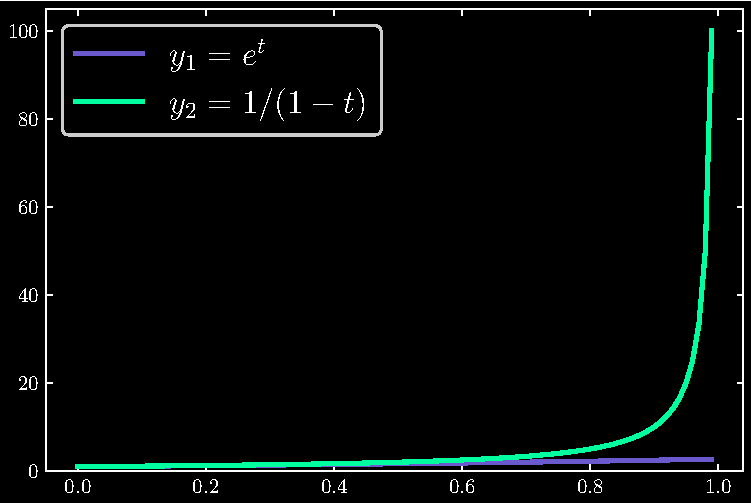
\includegraphics[width=1.0\textwidth]{../chap1/sec1.1/chap1sec1.1ex8.eps}
\end{center}

\qs{1.1.9}{Find a solution to \(dy/dt = -y^{2}\) starting from \(y \!\left( 0 \right) = 1\). Integrate \(dy/y^{2}\) and \(-dt\). (Or work with \(z = 1/y\). Then \(\bm{dz/dt} = \!\left( dz/dy \right) \!\left( dy/dt \right) = \!\left( -1/y^{2} \right) \!\left( -y^{2} \right) = \textbf{1}\). From \(dz/dt = 1\) you will know \(z \!\left( t \right) \) and \(y = 1/z\).}

\underline{Solution 1.} Write
\begin{alignat*}{2}
	&-\int \frac{1}{y^{2}} \ dy  && = \int  \ dt  \\
	&\implies y^{-1} && = t + C \\ 
	&\implies y && = \boxed{\frac{1}{t + C}, \quad C = 1}
\end{alignat*}

\underline{Solution 2.} Let \(z = 1/y\). Then
\[
	\frac{d z}{d t} = \frac{d z}{d y} \frac{d y}{d t} = \!\left( -\frac{1}{y^{2}} \right) \!\left( -y^{2} \right) = 1
\]
Since \(dz/dt = 1\),
\begin{align*}
	\int \ dz = \int \ dt & \implies z = t + C \\
	 & \implies \frac{1}{y} = t + C \\ 
	 & \implies \boxed{y = \frac{1}{t + C}, \quad C = 1}
\end{align*}

% QUESTION 10
\qs{1.1.10}{Which of these differential equations are linear (in \(y\))?\begin{enumerate}[label=(\alph*)]
	\item \(y' + \sin y = t\)
	\item \(y' = t^{2} \!\left( y-t \right) \)
	\item \(y' + e^{t}y = t^{10}\)
\end{enumerate}}

Only (b) and (c) are linear in \(y\).

\vspace{12pt}

% QUESTION 11
\qs{1.1.11}{The product rule gives what derivative for \(e^{t} e^{-t}\)? This function is constant. At \(t=0\) this constant is \(1\). Then \(e^{t}e^{-t} = 1\) for all \(t\).}

By the product rule, we have
\begin{align*}
	\frac{d }{d t} \!\left( e^{t}e^{-t} \right)  & = e^{-t} \frac{d }{d t} \!\left( e^{t} \right) + e^{t} \frac{d }{d t} \!\left( e^{-t} \right)  \\
	 & = \!\left( e^{-t} \right) \!\left( e^{t} \right) - \!\left( e^{t} \right) \!\left( e^{-t} \right)  \\ 
	 & = 0
\end{align*}

which aligns with the result that \(d(1)/dt = 0\).

% QUESTION 12
\qs{1.1.12}{\(dy/dt = y + 1\) is not solved by \(y = e^{t} + t\). Substitute that \(y\) to show it fails. We can't just add the solutions to \(y' = y\) and \(y' = 1\). What number \(c\) makes \(y = e^{t} + c\) into a correct solution?}

Observe that
\begin{align*}
	\frac{d }{d t} \!\left( e^{t} + t \right)   & = e^{t} + 1 \\
	 & \neq e^{t} + t + 1 \\ 
\end{align*}

If \(c = -1\), we have
\begin{align*}
	\frac{d }{d t} \!\left( e^{t} - 1 \right)   & = e^{t} \\
	 & = \!\left( e^{t} - 1 \right) + 1  \\ 
\end{align*}

\newpage
\subsection{\textsf{1.3 - The Exponentials \texorpdfstring{\(e^{t}\)}{e(t)} and \texorpdfstring{\(e^{at}\)}{exp(at)}}}

% QUESTION 1
\qs{1.3.1}{Set \(t = 2\) in the infinite series for \(e^{2}\). The sum must be \(e\) times \(e\), close to \(7.39\). How many terms in the series to reach a sum of \(7\)? How many terms to pass \(7.3\)?}

Five terms are needed to reach 7 exactly:
\[
	y = 1 + t + \frac{1}{2!}t^{2} + \frac{1}{3!}t^{3} + \frac{1}{4!}t^{4} = 7
\]
And seven terms to surpass 7.3:
\[
	y = 1 + t + \frac{1}{2!}t^{2} + \frac{1}{3!}t^{3} + \frac{1}{4!}t^{4} + \frac{1}{5!}t^{5} + \frac{1}{6!}t^{6} \approx 7.36
\]

\begin{python}
t = 2

term1 = 1
term2 = 1 + t
term3 = 1 + t + (1/2)*np.power(t,2)
term4 = 1 + t + (1/2)*np.power(t,2) + (1/6)*np.power(t,3)
term5 = 1 + t + (1/2)*np.power(t,2) + (1/6)*np.power(t,3) 
	+ (1/24)*np.power(t,4)
term6 = 1 + t + (1/2)*np.power(t,2) + (1/6)*np.power(t,3) 
	+ (1/24)*np.power(t,4) + (1/120)*np.power(t,5)
term7 = 1 + t + (1/2)*np.power(t,2) + (1/6)*np.power(t,3) 
	+ (1/24)*np.power(t,4) + (1/120)*np.power(t,5) 
	+ (1/720)*np.power(t,6)
\end{python}

% QUESTION 2
\qs{1.3.2}{Starting from \(y \!\left( 0 \right) = 1\), find the solution to \(dy/dt = y\) at time \(t = 1\). Starting from that \(y \!\left( 1 \right) \), solve \(dy/dt = -y\) to time \(t = 2\). Draw a rough graph of \(y \!\left( t \right) \) from \(t = 0\) to \(t = 2\). What does this say about \(e^{-1}\) times \(e\)?}

The solution to \(dy/dt = y\) is \(y = Ce^{t}\); since by premise we have \(y \!\left( 0 \right) = 1\), this implies \(C = 1\). Moreover, we have \(y \!\left( 1 \right) = e\). For \(dy/dt = -y\), we have solution \(y = De^{-t}\). Using \(y \!\left( 1 \right) = e\), we may conclude \(D = e^{2}\). Thus at \(t = 2\), \(y \!\left( 2 \right) = 1\). The complete solution is
\[
	y \!\left( t \right) =
	\begin{cases}
		e^{t} & 0 \le t \le 1 \\
		e^{2-t} & 1 < t \le 2 \\
	\end{cases}
\]
Graphically, we have:

\begin{center}
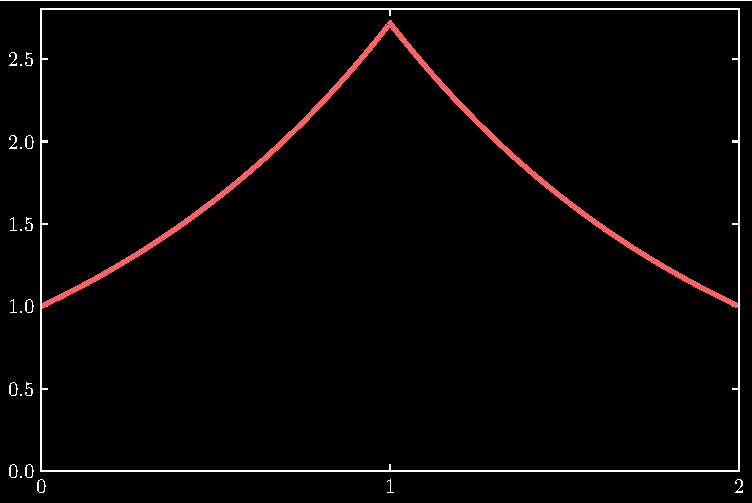
\includegraphics[width=1.0\textwidth]{../chap1/sec1.3/chap1sec1.3ex2.eps}
\end{center}

This implies that \(e^{-1} \cdot e = 1\).

\vspace{12pt}

% QUESTION 3
\qs{1.3.3}{Start with \(y \!\left( 0 \right) = \$5000\). If this grows by \(dy/dt = .02y\) until \(t = 5\) and then jumps to \(a = .04\) per year until \(t = 10\), what is the account balance at \(t = 10\)?}

The solution to \(dy/dt = .02y\) with \(y_{1} \!\left( 0 \right) = 5000\) is \(y_{1} = 5000e^{.02t}\), for \(0 \le t \le 5\). 

When the interest rate changes to \(.04\) at \(t = 5\), we must solve \(dy/dt = .04y\) and impose the initial constraint that \(y_{2} \!\left( 5 \right) = y_{1} \!\left( 5 \right) \). We can conclude that \(y_{2}\) is
\[
	y_{2} \!\left( t \right) = \!\left( \frac{5000e^{.02 \cdot 5}}{e^{.04 \cdot 5}} \right) e^{.04t} = \!\left( 5000e^{-.1} \right) e^{.04t} , \quad 5 < t \le 10
\]
Lastly, we calculate that at \(t = 10\), \(y \!\left( 10 \right) = \$6749.29\). Graphically, we have

\begin{center}
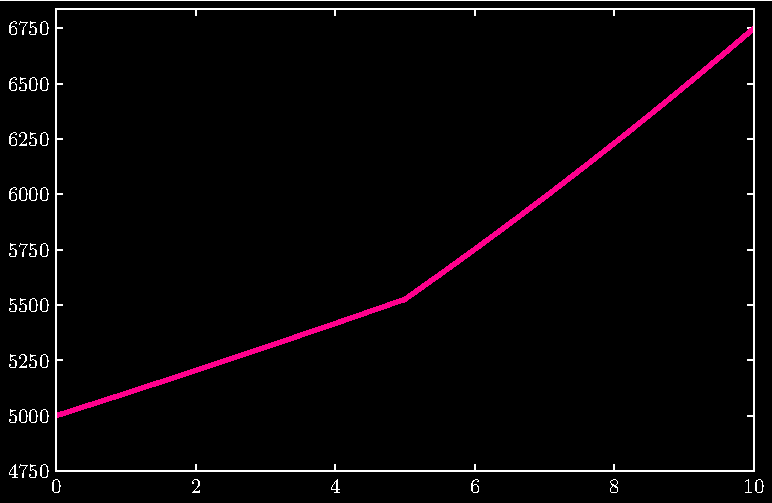
\includegraphics[width=1.0\textwidth]{../chap1/sec1.3/chap1sec1.3ex3.eps}
\end{center}

% QUESTION 4
\qs{1.3.4}{Change Problem 3 to start with \(\$5000\) growing at \(dy/dt = .04y\) for the first five years. Then drop to \(a = .02\) until \(t = 10\). What is now the balance at \(t = 10\)?}

Switching \(.02\) and \(.04\) in the previous problem, we derive the exact same balance of \(y \!\left( 10 \right) = \$6749.29\). The piecewise solutions are
\[
	y \!\left( t \right) =
	\begin{cases}
		y_{1} \!\left( t \right)  = 5000e^{.04t} & 0 \le t \le 5 \\
		y_{2} \!\left( t \right)  = \!\left( \frac{5000e^{.04 \cdot 5}}{e^{.02 \cdot 5}} \right) e^{.02t} & 5 < t \le 10 \\
	\end{cases}
\]

Graphically, we have

\begin{center}
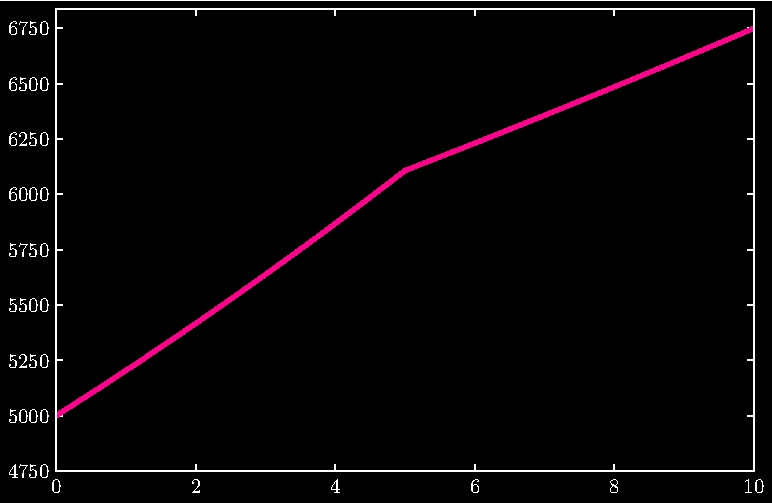
\includegraphics[width=1.0\textwidth]{../chap1/sec1.3/chap1sec1.3ex4.eps}
\end{center}

% QUESTION 5
\qs{1.3.5}{Replace \(t\) by \(at\) in the exponential series to find \(e^{at}\):
\[
	e^{at} = 1 + at + \frac{1}{2} \!\left( at \right)^{2} + \cdots + \frac{1}{n!} \!\left( at \right)^{n} + \cdots 
\]
Take the derivative of every term (keep five terms). Factor out \(a\) to show that \textit{the derivative of \(e^{at}\) equals \(ae^{at}\)}. At what time \(T\) does \(e^{at}\) reach 2?}

Derive
\begin{align*}
	\frac{d }{d t} e^{at} &= a + a \!\left( at \right) + \cdots + \frac{1}{\!\left( n-1 \right)!} a \!\left( at \right)^{n-1} + \cdots \\
			     &= a \!\left( 1 + at + \cdots + \frac{1}{\!\left( n-1 \right)!} \!\left( at \right)^{n-1} + \cdots \right) \\
			     &= ae^{at}
\end{align*}

For \(e^{aT} = 2\), calculate
\begin{alignat*}{2}
	\implies& aT && = \ln\!\left( 2 \right) \\
	\implies& T && = \boxed{ \frac{\ln\!\left( 2 \right)}{a} } \\ 
\end{alignat*}

\newpage
% QUESTION 6
\qs{1.3.6}{Start from \(y' = ay\). Take the derivative of that equation. Take the \(n^{\text{th}}\) derivative. Construct the Taylor series that matches all these derivatives at \(t = 0\), starting from \(1 + at + \frac{1}{2} \!\left( at \right)^{2}\). Confirm that this series for \(y \!\left( t \right) \) is the series for \(e^{at}\) in Problem 5.}

The derivative of \(y' = ay\) is:
\[
	y'' = ay'
\]
The \(n^{\textit{th}}\) derivative is:
\[
	y^{\!\left( n + 1 \right) } = ay^{\!\left( n \right) }
\]
Starting from \(1 + at + \frac{1}{2} \!\left( at \right)^{2}\), we observe that
\[
	y' = a + a \!\left( at \right) \quad \text{and} \quad ay = a \!\left( 1 + at + \frac{1}{2} \!\left( at \right)^{2} \right) 
\]
but as it stands, the two sides are unequal. If we add a term \(\frac{1}{3!} \!\left( at \right)^{3}\), we have
\[
	y' = a + a \!\left( at \right) + \frac{1}{2} a \!\left( at \right)^{2} \quad \text{and} \quad ay = a \!\left( 1 + at + \frac{1}{2} \!\left( at \right)^{2} + \frac{1}{3!} \!\left( at \right)^{3} \right) 
\]
In fact, we will need to continue adding terms of the form \(\frac{1}{n!} \!\left( at \right)^{n}\) ad infinitem. Observe that we derive the result of Problem 5 in this manner.

In general, the \(k^{\text{th}}\) derivative of the term \(\frac{1}{n!} \!\left( at \right)^{n}\) is
\[
	\frac{1}{\!\left( n-k \right)!} a^{k} \!\left( at \right)^{n-k}
\]
Then the equation \(y^{\!\left( n + 1 \right)} = ay^{\!\left( n \right) }\) is
\[
	a^{n + 1} + a^{n + 1} \!\left( at \right) + \frac{1}{2!} a^{n + 1} \!\left( at \right)^{2} + \cdots = a \!\left( a^{n} + a^{n} \!\left( at \right) + \frac{1}{2!} a^{n} \!\left( at \right)^{2} + \cdots \right) 
\]

% QUESTION 7
\qs{1.3.7}{At what times \(t\) do these events happen?
\begin{enumerate}[label=(\alph*)]
	\item \(e^{at} = e\)
	\item \(e^{at} = e^{2}\)
	\item \(e^{a \!\left( t + 2 \right) } = e^{at} e^{2a}\).
\end{enumerate}}

\par (a) \(t = 1/a\)
\vspace{12pt}
\par (b) \(t = 2/a\)
\vspace{12pt}
\par (c) \(t \ge 0\)

% QUESTION 8
\qs{1.3.8}{If you multiply the series for \(e^{at}\) in Problem 5 by itself you should get the series for \(e^{2at}\). Multiply the first 3 terms by the same 3 terms to see the first 3 terms in \(e^{2at}\).}
\begin{align*}
	\!\left( 1 + at + \frac{1}{2} \!\left( at \right)^{2} \right)^{2} &= \!\left( 1 + at + \frac{1}{2} \!\left( at \right)^{2} \right)  \\
	 & \quad + at \!\left( 1 + at + \frac{1}{2} \!\left( at \right)^{2} \right)  \\ 
	 & \quad + \frac{1}{2} \!\left( at \right)^{2} \!\left( 1 + at + \frac{1}{2} \!\left( at \right)^{2} \right) \\
	 & = 1 + 2at + 2 \!\left( at \right)^{2} + \!\left( at \right)^{3} + \frac{1}{2} \!\left( at \right)^{4}
\end{align*}

% QUESTION 9
\qs{1.3.9}{(recommended) Find \(y \!\left( t \right) \) if \(dy/dt = ay\) and \(\bm{y \!\left( T \right) = 1}\) (instead of \(y \!\left( 0 \right) = 1\)).}

The general solution is \(y \!\left( t \right) = Ce^{at}\). If \(y \!\left( T \right) = 1\), then \(C = e^{-aT}\).

\vspace{12pt}

% QUESTION 10
\qs{1.3.10}{\begin{enumerate}[label=(\alph*)]
	\item If \(dy/dt = \!\left( \ln 2 \right)y \), explain why \(y \!\left( 1 \right) = 2 y \!\left( 0 \right) \).
	\item If \(dy/dt = - \!\left( \ln 2 \right)y \), how is \(y \!\left( 1 \right) \) related to \(y \!\left( 0 \right) \)?
\end{enumerate}}

\par (a) We have \(y \!\left( t \right) = e^{\!\left( \ln 2 \right) t} = 2^{t}\). Then \(y \!\left( 1 \right) = 2\) and \(y \!\left( 0 \right) = 1\). Thus 
\[
	y \!\left( 1 \right) = 2 y \!\left( 0 \right) 
\]
\par (b) We have \(y \!\left( t \right) = 1/2^{t}\). Then \(y \!\left( 1 \right) = 1/2\) and \(y \!\left( 0 \right) = 1\). Thus 
\[
	2 y \!\left( 1 \right) = y \!\left( 0 \right)
\]

% QUESTION 11
\qs{1.3.11}{In a one-year investment of \(y \!\left( 0 \right) = \$100\), suppose the interest rate jumps from \(6\%\) to \(10 \%\) after six months. Does the equivalent rate for a whole year equal \(8 \%\), or more than \(8 \%\), or less than \(8 \%\)?}

The initial condition \(y \!\left( 0 \right) = \$100\) implies \(C = 100\) for the solution \(y_{1} \!\left( t \right) = Ce^{.06t}\). To find the initial condition on \(y_{2} \!\left( t \right) = De^{.1t}\), we must have
\[
	y_{1} \!\left( 6 \right) = 100e^{.06 \cdot 6} = y_{2} \!\left( 6 \right) = De^{.1 \cdot 6}
\]
implying that \(D = 100 e^{-.24}\). The piecewise solutions are
\[
	y \!\left( t \right) = \begin{cases}
		y_{1} \!\left( t \right) = 100e^{.06t}  & 0 \le t \le 6 \\
		y_{2} \!\left( t \right) = \!\left( 100e^{-.24} \right) e^{.1t} & 6 < t \le 12  \\
	\end{cases}
\]

Now, in the event where the interest rate is 8 percent, we can simply determine that the value of our balance at 12 months is
\[
	y \!\left( 12 \right) = 100e^{.8 \cdot 12} = 100e^{.96}
\]
Similarly, in the first case with the two interest rates, we calculate
\[
	y \!\left( 12 \right) = \!\left( 100e^{-.24} \right) e^{.1 \cdot 12} = 100e^{.96}
\]
demonstrating that the end balances are identical in both schemes. Graphically:

\begin{center}
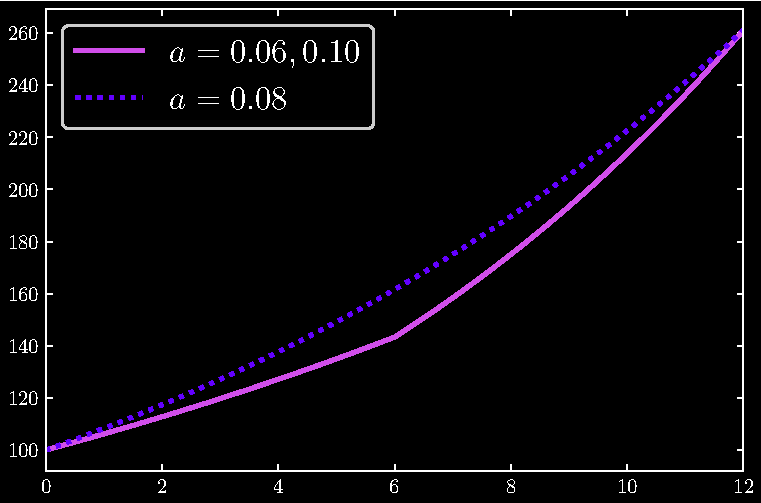
\includegraphics[width=1.0\textwidth]{../chap1/sec1.3/chap1sec1.3ex11.eps}
\end{center}

% QUESTION 12
\qs{1.3.12}{If you invest \(y \!\left( 0 \right) = \$100\) at \(4 \%\) interest compounded continuously, then \(dy/dt = .04y\). Why do you have more than \(\$104\) at the end of the year?}

We have solution \(y \!\left( t \right) = 100e^{.04t}\). Since \(e^{.04} > 1.04\), we will have in excess of \(\$104\) at the close of the year.

\vspace{12pt}

\newpage
% QUESTION 13
\qs{1.3.13}{What linear differential equation \(dy/dt = a \!\left( t \right) y\) is satisfied by \(y \!\left( t \right) = e^{\cos t}\)?}

The linear differential equation is satisfied with \(a \!\left( t \right) = -\sin t \).

\vspace{12pt}

% QUESTION 14
\qs{1.3.14}{If the interest rate is \(a = 0.1\) per year in \(y' = ay\), how many years does it take for your investment to be multiplied by \(e\)? How many years to be multiplied by \(e^{2}\)?}

The solution is \(y \!\left( t \right) = C e^{at}\). For any initial investment \(C\), we wish to find \(t_{1}\) such that \(y \!\left( t_{1} \right) = Ce^{at_{1}} = Ce\). It follows that \(t_{1} = 1/a = 10\) years. Similarly, we can derive \(t_{2}\) such that \(y \!\left( t_{2} \right) = Ce^{at_{2}} = Ce^{2}\) as \(t_{2} = 2/a = 20\) years.

\vspace{12pt}

% QUESTION 15
\qs{1.3.15}{Write the first four terms in the series for \(y = e^{t^{2}}\). Check that \(dy/dt = 2ty\).}

By the Taylor series expansion of the exponential function, we have
\begin{align*}
	y = e^{t^{2}} & = 1 + \!\left( t^{2} \right) + \frac{1}{2!} \!\left( t^{2} \right)^{2} + \frac{1}{3!} \!\left( t^{2} \right)^{3} + \cdots \\
		     & = 1 + t^{2} + \frac{1}{2!} t^{4} + \frac{1}{3!} t^{6} + \cdots 
\end{align*}

with derivative
\begin{align*}
	\frac{d y}{d t} & = 2t + \frac{4}{2!} t^{3} + \frac{6}{3!} t^{5} + \frac{8}{4!} t^{7} + \cdots  \\
	 & = 2t \!\left( 1 + t^{2} + \frac{1}{2!} t^{4} + \frac{1}{3!} t^{6} + \cdots  \right)  \\ 
	 & = 2ty
\end{align*}

% QUESTION 16
\qs{1.3.16}{Find the derivative of \(Y \!\left( t \right) = \!\left( 1 + \frac{t}{n} \right)^{n}\). If \(n\) is large, this \(dY/dt\) is close to \(Y\)!}

We have
\[
	\frac{d Y}{d t} = n \!\left( 1 + \frac{t}{n} \right)^{n-1} \!\left( \frac{1}{n} \right) = \!\left( 1 + \frac{t}{n} \right)^{n-1}
\]
As \(n \rightarrow \infty\), \(n \approx n-1\), \(1 + t/n \approx 1\), and \(dY/dt \approx Y\).

% QUESTION 17
\qs{1.3.17}{Suppose the exponent in \(y = e^{u \!\left( t \right) }\) is \(u \!\left( t \right) = \) integral of \(a \!\left( t \right) \). What equation \(dy/dt = \underline{\qquad} \ y\) does this solve? If \(u \!\left( 0 \right) = 0\) what is the starting value \(y \!\left( 0 \right) \)?}

The solution \(y\) solves \(dy/dt = a \!\left( t \right) y\). The initial condition \(u \!\left( 0 \right) = 0\) implies \(y \!\left( 0 \right) = e^{u \!\left( 0 \right) } = 1 \).

\vspace{12pt}

% QUESTION 18
\qs{1.3.18}{\(e^{d/dx} = 1 + d/dx + \frac{1}{2} \!\left( d/dx \right)^{2} + \cdots\) is a sum of higher and higher derivatives. Applying this series to \(f \!\left( x \right) \) at \(x = 0\) would give \(f + f' + \frac{1}{2} f'' + \cdots \) at \(x = 0\). The Taylor series says: This is equal to \(f \!\left( x \right) \) at \(x = \underline{\qquad}\).}

It is clearer if we say that we apply the series to \(f \!\left( a \right) \) at point \(a = 0\). The definition of the Taylor series about the point \(a = 0\) is given by
\[
	\sum_{n=0}^{\infty} \frac{f^{\!\left( n \right) } \!\left( 0 \right) }{n!} x^{n}
\]
Then when \(x = 1\), the Taylor (Maclaurin) series is equal to \(f \!\left( 1 \right) \):
\[
	f \!\left( 1 \right) = f + f' + \frac{1}{2} f'' + \cdots
\]
% QUESTION 19
\qs{1.3.19}{(Computer or calculator, 2.xx is close enough) Find the time \(t\) when \(e^{t} = 10\). The initial \(y \!\left( 0 \right) \) has increased by an order of magnitude - a factor of 10. The exact statement of the answer is \(t = \underline{\qquad}\). At what time \(t\) does \(e^{t}\) reach 100?}

The time \(t\) when \(e^{t} = 10\) is \(t \approx 2.30\). It is exactly \(t = \ln 10\). We reach \(e^{t} = 100\) when \(t = \ln 100 \approx 4.61\).

\vspace{12pt}

% QUESTION 20
\qs{1.3.20}{The most important curve in probability is the bell-shaped graph of \(e^{-t^{2}/2}\). With a calculator or computer find this function at \(t = -2, -1, 0, 1, 2\). Sketch the graph of \(e^{-t^{2}/2}\) from \(t = -\infty\) to \(t = \infty\). \textit{It never goes below zero.}}

The function \(e^{-t^{2}/2}\) at \(t = -2, -1, 0, 1, 2\) is \(0.135, 0.607, 1, 0.607, 0.135\). The graph is

\begin{center}
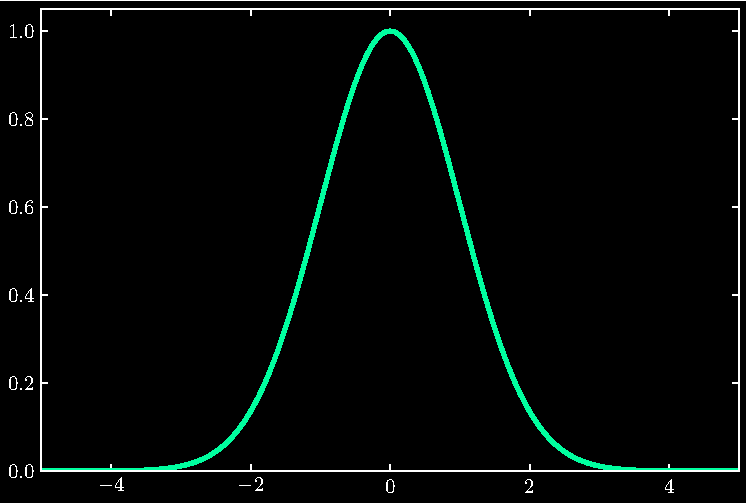
\includegraphics[width=1.0\textwidth]{../chap1/sec1.3/chap1sec1.3ex20.eps}
\end{center}

% QUESTION 21
\qs{1.3.21}{Explain why \(y_{1} = e^{\!\left( a + b + c \right) t}\) is the same as \(y_{2} = e^{at} e^{bt} e^{ct}\). They both start at \(y \!\left( 0 \right) = 1.\) They both solve what differential equation?}

Consider the differential equation
\[
	\frac{d y}{d t} = \!\left( a + b + c \right) y
\]
Then by property 1 of the exponential function,
\[
\frac{d y_{1}}{d t} = \!\left( a + b + c\right) e^{\!\left( a + b + c \right)t}  = \!\left( a + b + c \right) y_{1}
\]
Using the product rule, we can also derive from \(y_{2}\):
\begin{align*}
	\frac{d y_{2}}{d t} & = e^{at}e^{bt} \frac{d }{d t} e^{ct} + e^{ct} \frac{d }{d t} \!\left( e^{at}e^{bt} \right) \\
			   & = c y_{2} + e^{ct} \!\left( e^{at} \frac{d }{d t} e^{bt} + e^{bt} \frac{d }{d t} e^{at} \right) \\
			   & = c y_{2} + b y_{2} + a y_{2} \\
			   & = \!\left( a + b + c \right) y_{2}
\end{align*}

ascertaining that \(y_{1} = y_{2}\).

The second method is to begin at \(y \!\left( 0 \right) = 1\), and go to \(e^{at}\). Let \(C = e^{at}\). Then move an additional \(e^{bt}\) and arrive at \(Ce^{bt}\). Let \(D\) equal this, and make one final additional move of \(e^{ct}\). In total, we have grown by a factor of \(e^{at}e^{bt}e^{ct}\). But this is equal to moving ahead in time by \(at + bt + ct = \!\left( a + b + c \right) t\).

% QUESTION 22
\qs{1.3.22}{For \(y' = y\) with \(a = 1\), Euler's first step chooses \(Y_{1} = \!\left( 1 + \Delta t \right) Y_{0} \). Backward Euler chooses \(Y_{1} = Y_{0} / \!\left( 1 - \Delta t \right) \). Explain why \(1 + \Delta t\) is smaller than the exact \(e^{\Delta t}\) and \(1/\!\left( 1 - \Delta t \right) \) is larger than \(e^{\Delta t}\). (Compare the series for \(1/\!\left( 1 - x \right) \) with \(e^{x}\).

\vspace{12pt}
\textbf{Note} Section 3.5 presents an accurate Runge-Kutta method that captures three more terms of \(e^{a \Delta t}\) than Euler. For \(dy/dt = ay\) here is the step to \(Y_{n+1}\):

\vspace{12pt}
\textbf{Runge-Kutta for \(\bm{y' = ay}\)}  
\[
	Y_{n+1} = \!\left( 1 + a \Delta t + \frac{a^{2} \Delta t^{2}}{2} + \frac{a^{3} \Delta t^{3}}{6} + \frac{a^{4} \Delta t^{4}}{24} \right) Y_{n}
\]}

First, observe that
\[
	1 + \Delta t < 1 + \Delta t + \frac{1}{2!} \!\left( \Delta t \right)^{2} + \frac{1}{3!} \!\left( \Delta t \right)^{3} + \cdots = e^{\Delta t}
\]
Allowing us to conclude that \(1 + \Delta t < e^{\Delta t}\).

Next, consider the Taylor series for \(1/\!\left( 1-x \right) \):
\[
	\frac{1}{1-x} = 1 + x + x^{2} + x^{3} + \cdots = \sum_{n=0}^{\infty} x^{n}
\]
Backward Euler gives us
\[
	\frac{1}{1 - \Delta t} = 1 + \Delta t + \!\left( \Delta t \right)^{2} + \!\left( \Delta t \right)^{3} + \cdots 
\]
while the Taylor expansion of \(e^{\Delta t}\) gives us
\[
	e^{\Delta t} = 1 + \Delta t + \frac{1}{2!} \!\left( \Delta t \right)^{2} + \frac{1}{3!} \!\left( \Delta t \right)^{3} + \cdots
\]
which ascertains that \(1 / \!\left( 1 - \Delta t \right) > e^{\Delta t}\). 

\newpage
\subsection{\textsf{1.4 - Four Particular Solutions}}

% QUESTION 1
\qs{1.4.1}{All solutions to \(dy/dt = -y + 2\) approach the steady state where \(dy/dt\) is zero and \(y = y_{\infty} = \underline{\qquad}\). That constant \(y = y_{\infty}\) is a particular solution \(y_{p}\).

Which \(y_{n} = Ce^{-t}\) combines with this steady state \(y_{p}\) to start from \(y \!\left( 0 \right) = 4\)? This question chose \(y_{p} + y_{n}\) to be \(y_{\infty} + \)\textit{transient} (decaying to zero).}

Derive
\begin{alignat*}{3}
	&\implies && \frac{dy}{dt} + y && = 2 \\
	&\implies && e^{t} \!\left( y' + y \right) && = 2e^{t} \\
	&\implies && \frac{d }{d t} \!\left( e^{t} y \right) && = 2e^{t} \\
	&\implies && e^{t} y \!\left( t \right) - y \!\left( 0 \right) && = \int^{t}_{0} 2e^{s} \ ds \\
	& && && = 2 \!\left( e^{t} - 1 \right) \\
	&\implies && y \!\left( t \right) && = e^{-t} y \!\left( 0 \right) - 2 \!\left( e^{-t} - 1 \right) 
\end{alignat*}

Thus as \(t \rightarrow \infty\), we have \(y \!\left( t \right) \rightarrow 2 = y_{\infty}\). For \(y \!\left( 0 \right) = 4\), we have \(y_{n} = 4e^{-t}\) and \(y_{p} = -2 \!\left( e^{-t} - 1 \right) \), leaving us with the complete solution
\[
	y \!\left( t \right) = \underbrace{2}_{\text{steady}} + \underbrace{2e^{-t}}_{\text{transient}}
\]

% QUESTION 2
\qs{1.4.2}{For the same equation \(dy/dt = -y + 2\), choose the null solution \(y_{n}\) that starts from \(y \!\left( 0 \right) =4\). Find the particular solution \(y_{p}\) that starts from \(y \!\left( 0 \right) = 0\).

This splitting chooses the two parts \(e^{at} y \!\left( 0 \right) + \) integral of \(e^{a \!\left( t-s \right) }q\) in equation (4).}

Since \(y_{n} \!\left( 0 \right) = 4\), we have \(y_{n} \!\left( t \right) = 4e^{-t}\). The particular solution is \(y_{p} \!\left( t \right) = -2 \!\left( e^{-t} - 1 \right) \), from which we can determine \(y_{p} \!\left( 0 \right) = 0\).
\vspace{12pt}

% QUESTION 3
\qs{1.4.3}{The equation \(dy/dt = -2y + 8\) has two natural splittings \(\bm{y_{S} + y_{T} = y_{N} + y_{P}:}\)

\textbf{1.} Steady \(\bm{\!\left( y_{S} = y_{\infty} \right) } + \text{Transient} \bm{\!\left( y_{T} \rightarrow 0 \right) }\). What are those parts if \(y \!\left( 0 \right) = 6\)?

\textbf{2.} \( ( y'_{N} = -2y_{N}\) from \(\bm{y_{N} \!\left( 0 \right) = 6} ) + ( y'_{P} = -2y_{P} + 8\) starting from \( \bm{y_{P} \!\left( 0 \right) = 0} )  \).}

1) Derive
\begin{alignat*}{3}
	 &\implies && \!\left( y' + 2y \right) && = 8  \\
	 &\implies && e^{2t} \!\left( y' + 2y \right) && = 8e^{2t}   \\ 
	 &\implies && \frac{d }{d t} \!\left( e^{2t}y \right) && = 8e^{2t} \\
	 &\implies && e^{2t} y \!\left( t \right) - y \!\left( 0 \right) && = \int^{t}_{0} 8e^{2s} \ ds \\
	 &\implies && y \!\left( t \right) && = 6e^{-2t} - 4 \!\left( e^{-2t} - 1 \right) 
\end{alignat*}

which gives us steady and transient parts:
\[
	y \!\left( t \right) = \underbrace{4}_{\text{steady}} + \underbrace{2e^{-2t}}_{\text{transient}}
\]

2) We can also think of splitting \(y \!\left( t \right) \) into its constituent null and particular solutions. For the null we have
\[
	y_{N} \!\left( t \right) = 6e^{-2t}
\]
which conforms to the initial condition \(y_{N} \!\left( 0 \right) = 6\) and solves \(y_{N}' = -2y_{N}\). Now, the particular solution is
\[
	y_{P} = -4 \!\left( e^{-2t} - 1 \right) 
\]
which conforms to the initial condition \(y_{P}\!\left( 0 \right) = 0\) and solves \(y_{P}' = -2y_{P} + 8\).

\vspace{12pt}

% QUESTION 4
\qs{1.4.4}{All null solutions to \(u - 2v = 0\) have the form \(\!\left( u,v \right) = \!\left( c, \underline{\qquad} \right) \).
\vspace{12pt}

One particular solution to \(u - 2v = 3\) has the form \(\!\left( u,v \right) = \!\left( 7, \underline{\qquad} \right) \).
\vspace{12pt}

Every solution to \(u - 2v = 3\) has the form \(\!\left( 7, \underline{\qquad} \right) + c \!\left( 1, \underline{\qquad} \right) \).
\vspace{12pt}

But also every solution has the form \(\!\left( 3, \underline{\qquad} \right) + C \!\left( 1, \underline{\qquad} \right) \) for \(C = c+4\).}

\begin{align*}
	\!\left( u,v \right) & = \!\left( c, c/2 \right) \\
	\!\left( u,v \right) & = \!\left( 7,2 \right) \\
	\!\left( 7,2 \right) & + c \!\left( 1, 1/2 \right) \\
	\!\left( 3,0 \right) & + C \!\left( 1,1/2 \right) 
\end{align*}

In the fourth solution, recognize that we may write 
\[
	\!\left( c + 4 \right) \!\left( 1, 1/2 \right) = \!\left( c + 4, c/2 + 2 \right) 
\] 
But in using the third solution, we can subtract \(\!\left( 4,2 \right) \) from \(\!\left( 7,2 \right) \) to get \(\!\left( 3,0 \right) \).

\vspace{12pt}

% QUESTION 5
\qs{1.4.5}{The equation \(dy/dt = 5\) with \(y \!\left( 0 \right) = 2\) is solved by \(y = \underline{\qquad}\). A natural splitting \(y_{n} \!\left( t \right) = \underline{\quad}\) and \(y_{p} \!\left( t \right) = \underline{\quad}\) comes from \(y_{n} = e^{at} y \!\left( 0 \right) \) and \(y_{p} \int e^{a \!\left( t-s \right) }5 \ ds\).

This small example has \(\bm{a = 0}\) (so \(ay\) is absent) and \(\bm{c = 0}\) (the source is \(q = 5e^{0t}\)). When \(a = c\) we have "resonance." A factor \(t\) will appear in the solution \(y\).}

We integrate both sides to derive
\begin{align*}
	y \!\left( t \right) - y \!\left( 0 \right)  & = \int^{t}_{0} 5  \ ds  \\
	\implies y \!\left( t \right)  & = 2 + 5t 
\end{align*}

where \(y_{n} \!\left( t \right) = 2\) and \(y_{p} \!\left( t \right) = 5t\).

\vspace{12pt}

\textbf{Starting with Problem 6, choose the very particular \(\bm{y_{p}}\) that starts from \(\bm{y_{p} \!\left( 0 \right) = 0}\).}

% QUESTION 6
\qs{1.4.6}{For these equations starting at \(y \!\left( 0 \right) = 1\), find \(y_{n} \!\left( t \right) \) and \(y_{p} \!\left( t \right) \) and \(y \!\left( t \right) = y_{n} + y_{p}\).

\begin{enumerate}[label=(\alph*)]
	\item \(y' - 9y = 90\)
	\item \(y' + 9y = 90\)
\end{enumerate}}

a) Derive
\begin{alignat*}{3}
	&\implies && e^{-9t} \!\left( y' - 9y \right) && = 90e^{-9t} \\
	&\implies && \frac{d }{d t} \!\left( e^{-9t}y \right) && = 90e^{-9t} \\ 
	&\implies && e^{-9t} y \!\left( t \right) - y \!\left( 0 \right) && = -10 \!\left( e^{-9t} - 1 \right) \\
	&\implies && y \!\left( t \right) && = e^{9t} y \!\left( 0 \right) + 10 \!\left( e^{9t} - 1 \right) \\
	& && && = \underbrace{e^{9t}}_{y_{n}} + \underbrace{10 \!\left( e^{9t} - 1 \right)}_{y_{p}} \\
	& && && = -10 + 11e^{9t}
\end{alignat*}

b) Derive
\begin{alignat*}{3}
	&\implies && e^{9t} \!\left( y' + 9y \right) && = 90e^{9t} \\
	&\implies && \frac{d }{d t} \!\left( e^{9t}y \right) && = 90e^{9t} \\ 
	&\implies && e^{9t}y \!\left( t \right) - y \!\left( 0 \right) && = 10 \!\left( e^{9t} - 1 \right) \\
	&\implies && y \!\left( t \right) && = \underbrace{e^{-9t}}_{y_{n}} \underbrace{- 10 \!\left( e^{-9t} - 1 \right) }_{y_{p}} \\
	& && && = 10 - 9e^{-9t}
\end{alignat*}

% QUESTION 7
\qs{1.4.7}{Find a linear differential equation that produces \(y_{n} \!\left( t \right) = e^{2t}\) and \(y_{p} \!\left( t \right) = 5 \!\left( e^{8t} - 1 \right) \).}

Since \(y_{n} \!\left( t \right) = e^{2t}\), this implies that the homogeneous equation is
\[
	y' - 2y = 0
\]
Inputting the particular solution here gives us
\begin{align*}
	y_{p}' - 2y_{p} & = 40 e^{8t} - 10 \!\left( e^{8t} - 1 \right) \\
			& = 10 + 30 e^{8t}
\end{align*}
and so the linear differential equation is \(y \!\left( t \right) = 10 + 30 e^{8t}\). I seem to disagree with Strang's solutions manual here.

\vspace{12pt}

% QUESTION 8
\qs{1.4.8}{Find a resonant equation \(\!\left( a = c \right) \) that produces \(y_{n} \!\left( t \right) = e^{2t}\) and \(y_{p} \!\left( t \right) = 3te^{2t}\).}

The null solution implies the homogeneous equation
\[
	y' - 2y = 0
\]
Inputting the particular solution yields
\[
	3 \!\left( 2te^{2t} + e^{2t} \right) - 6te^{2t} = 3e^{2t}
\]
giving us the resonant equation
\[
	y \!\left( t \right) = 2y + 3e^{2t}
\]
with \(a = c = 2\). Intuitively, since the source has a factor of three, so must the particular solution.

\vspace{12pt}

% QUESTION 9
\qs{1.4.9}{\(y' = 3y + e^{3t}\) has \(y_{n} = e^{3t} y \!\left( 0 \right) \). Find the resonant \(y_{p}\) with \(y_{p} \!\left( 0 \right) = 0\).}

Here \(a = c = 3\). We find
\begin{align*}
	y \!\left( t \right) & = e^{3t} y \!\left( 0 \right) + e^{3t} \int^{t}_{0} \ ds \\
			   & = e^{3t} y \!\left( 0 \right) + te^{3t}
\end{align*}

Thus \(y_{p} \!\left( t \right) = t e^{3t}\).

\vspace{12pt}

\textbf{Problems 10-13 are about \(\bm{y'-ay =}\) constant source \(\bm{q}\).}

% QUESTION 10
\qs{1.4.10}{Solve these linear equations in the form \(y = y_{n} + y_{p}\) with \(y_{n} = y \!\left( 0 \right) e^{at}\).

\begin{enumerate}[label=(\alph*)]
	\item \(y' - 4y = -8\)
	\item \(y' + 4y = 8\)
\end{enumerate}
Which one has a steady state?}

(a) Derive
\begin{alignat*}{3}
	&\implies && e^{-4t} \!\left( y' - 4y \right) && = 8e^{-4t} \\
	&\implies && \frac{d }{d t} \!\left( e^{-4t}y \right) && = 8e^{-4t} \\ 
	&\implies && e^{-4t} y \!\left( t \right) - y \!\left( 0 \right) && = 8 \int^{t}_{0} e^{-4s} \ ds \\
	& && && = -2 \!\left( e^{-4t} - 1 \right) \\
	&\implies && y \!\left( t \right) && = \underbrace{e^{4t} y \!\left( 0 \right)}_{y_{n}} + \underbrace{2 \!\left( e^{4t} - 1 \right)}_{y_{p}}
\end{alignat*}

(b) Derive
\begin{alignat*}{3}
	&\implies && e^{4t} \!\left( y' + 4y \right) && = 8e^{4t} \\
	&\implies && \frac{d }{d t} \!\left( e^{4t}y \right) && = 8e^{4t} \\ 
	&\implies && e^{4t} y \!\left( t \right) - y \!\left( 0 \right) && = 8 \int^{t}_{0} e^{4s} \ ds \\
	& && && = 2 \!\left( e^{4t} - 1 \right) \\
	&\implies && y \!\left( t \right) && = \underbrace{e^{-4t} y \!\left( 0 \right) }_{y_{n}} \underbrace{-2 \!\left( e^{-4t} - 1 \right) }_{y_{p}}
\end{alignat*}

Since \(\lim\limits_{t \to \infty} y \!\left( t \right) = 2\), the differential equation in (b) has a steady state.

\vspace{12pt}

% QUESTION 11
\qs{1.4.11}{Find a formula for \(y \!\left( t \right) \) with \(y \!\left( 0 \right) = 1\) and draw its graph. What is \(y_{\infty}\)?
			
\begin{enumerate}[label=(\alph*)]
	\item \(y' + 2y = 6\)
	\item \(y' + 2y = -6\)
\end{enumerate}}

(a) Derive
\begin{alignat*}{3}
	&\implies && e^{2t} \!\left( y' + 2y \right) && = 6 e^{2t} \\
	&\implies && \frac{d }{d t} \!\left( e^{2t}y \right) && = 6e^{2t}  \\
	&\implies && e^{2t}y \!\left( t \right) - y \!\left( 0 \right) && = 6 \int^{t}_{0} e^{2s} \ ds \\
	& && && = 3 \!\left( e^{2t} - 1 \right) \\
	&\implies && y \!\left( t \right) && = \underbrace{e^{-2t}}_{y_{n}} \underbrace{- 3 \!\left( e^{-2t} - 1 \right) }_{y_{p}} \\
	& && && = -2e^{-2t} + 3
\end{alignat*}

with \(y_{\infty} = \lim\limits_{t \to \infty} = 3\).

(b) Since the forcing term has a sign change, we have complete solution
\[
	y \!\left( t \right) = \underbrace{e^{-2t}}_{y_{n}} + \underbrace{3 \!\left( e^{-2t} - 1 \right)}_{y_{p}} = 4e^{-2t} - 3
\]
with \(y_{\infty} = \lim\limits_{t \to \infty} = -3\).

\begin{center}
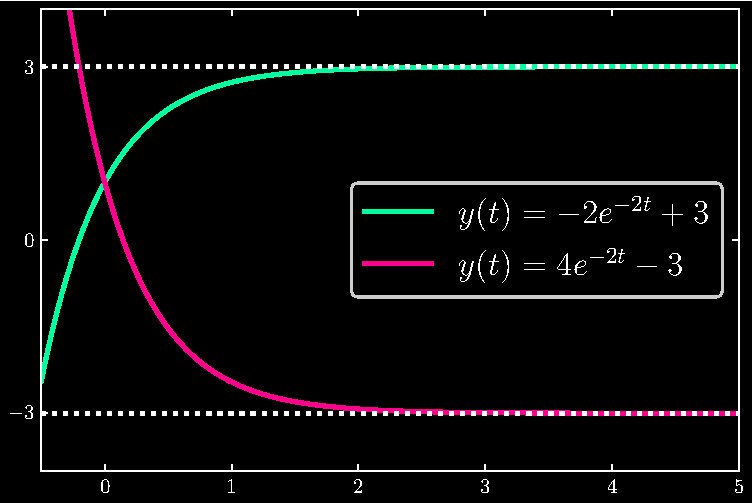
\includegraphics[width=1.0\textwidth]{../chap1/sec1.4/chap1sec1.4ex11.eps}
\end{center}

% QUESTION 12
\qs{1.4.12}{Write the equations in Problem 11 as \(Y' = -2Y\) with \(Y = y - y_{\infty}\). What is \(Y \!\left( 0 \right) \)?}

By premise, \(Y = y - y_{\infty} = y - 3\) in the case of equation (a). Then \(Y' = y'\) and \(-2Y = -2 \!\left( y-3 \right) \). Then we may rewrite \(y' + 2y = 6\) as
\[
	\begin{aligned}
		Y' = y' &= -2y + 6  \\
		 & = -2 \!\left( y - 3 \right)  \\
		 & = -2 Y
	\end{aligned}
\]

Analogously, for equation (b), we have \(Y = y - y_{\infty} = y + 3\) and rewrite in form

\[
	\begin{aligned}
		Y' = y' &= -2y - 6  \\
		 &= -2 \!\left( y + 3 \right)  \\
		 &= -2Y
	\end{aligned}
\]

We define \(Y \!\left( 0 \right) = y \!\left( 0 \right) - y_{\infty}\). Since \(y \!\left( 0 \right) = 1\), in the case of (a), \(Y \!\left( 0 \right) = 1 - 3 = 2\), and for (b), \(Y \!\left( 0 \right) = 1 + 3 = 4\). Thus the rewritten forms of the equations are the same, albeit with differing initial conditions.

\vspace{12pt}

% QUESTION 13
\qs{1.4.13}{If a drip feeds \(q = 0.3\) grams per minute into your arm, and your body eliminates the drug at the rate \(6y\) grams per minute, what is the steady state concentration \(y_{\infty}\)? Then \(in = out\) and \(y_{\infty}\) is constant. Write a differential equation for \(Y = y - y_{\infty}\).}

By premise, \(y' = -6y\). Moreover, with a source \(q = 0.3\), we can conclude the differential equation before us is
\[
	y' = -6y + 0.3
\]

Assuming that the body begins with zero concentration of the drug (i.e. \(y \!\left( 0 \right) = 0\), we solve

\begin{alignat*}{3}
	&\implies && e^{6t} \!\left( y' + 6y \right)  && = 0.3 e^{6t} \\
	&\implies && \frac{d }{d t} \!\left( e^{6t}y \right)  && = 0.3 e^{6t} \\
	&\implies && e^{6t} y \!\left( t \right) && = 0.3 \int^{t}_{0} e^{6s} \ ds \\
	& && && = 0.05 \!\left( e^{6t} - 1 \right) \\
	&\implies && y \!\left( t \right) && = \underbrace{- 0.05 \!\left( e^{-6t} - 1 \right) }_{y_{p}} \\
	& && && = -0.05 e^{-6t} + 0.05
\end{alignat*}

Taking the limit gives us \(\lim\limits_{t \to \infty} y \!\left( t \right) = y_{\infty} = 0.05\). Thus the steady state drug mass in the bloodstream is \boxed{0.05 \text{ grams}}.

\begin{center}
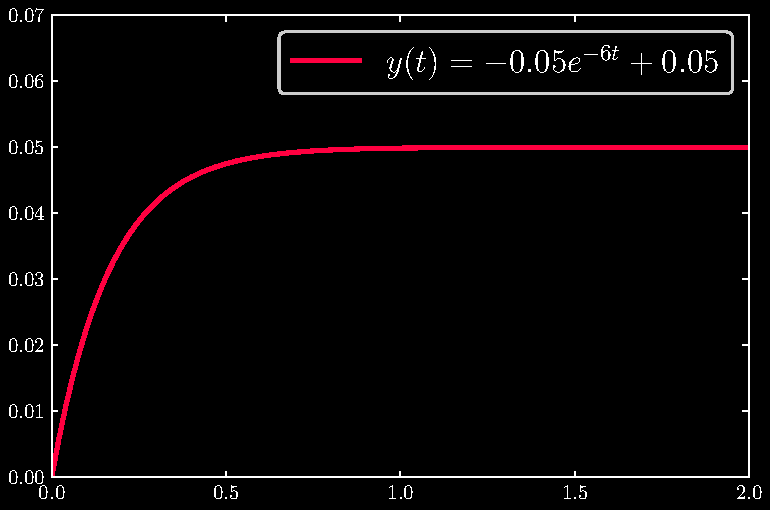
\includegraphics[width=1.0\textwidth]{../chap1/sec1.4/chap1sec1.4ex13.eps}
\end{center}

Then we define \(Y = y - y_{\infty} = y - 0.05\), with \(Y' = y'\) and as such,
\begin{align*}
	Y' = y' & = -6y + 0.3 \\
	 & = -6 \!\left( y - 0.05 \right)  \\ 
	 & = -6 Y
\end{align*}

% QUESTION 14
\qs{1.4.14}{Why is \(y_{\infty}\) the same for \(y' + y = H \!\left( t-2 \right) \) and \(y' + y = H \!\left( t - 10 \right) \)?}

We begin with the first equation, which multiplied by integrating factor \(e^{t}\) yields:

\begin{alignat*}{3}
	&\implies && \!\left( e^{t} y \right)' && = e^{t} H \!\left( t - 2 \right)   \\
	&\implies && e^{t} y \!\left( t \right) - y \!\left( 0 \right) && = \int^{t}_{2} e^{s} \ ds   \\
	& && && = e^{t} - e^{2} \\
	&\implies && y \!\left( t \right) && = e^{-t} y \!\left( 0 \right) - \!\left( e^{2 - t} - 1 \right)
\end{alignat*}

Taking the limit as \(t \rightarrow \infty\), we find
\[
	\lim\limits_{t \to \infty} y \!\left( t \right) = 1
\]

Next, we find for the second equation, with integrating factor \(e^{t}\):

\begin{alignat*}{3}
	&\implies && \!\left( e^{t}y \right)' && = e^{t} H \!\left( t - 10 \right)  \\
	&\implies && e^{t} y \!\left( t \right) - y \!\left( 0 \right) && = \int^{t}_{10} e^{s} \ ds  \\ 
	&  && && = e^{t} - e^{10} \\
	&\implies && y \!\left( t \right) && = e^{-t} y \!\left( 0 \right) - \!\left( e^{10 - t} - 1 \right) 
\end{alignat*}

Analogously, we also find
\[
	\lim\limits_{t \to \infty} y \!\left( t \right)  = 1
\]
Intuitively, if we think of the Heaviside function as a switch, all that differs between the two equations is when we ``turn on" the switch to the source. The source itself has the same magnitude across the two equations, so there is no reason for the limiting behavior of \(y \!\left( t \right) \) to deviate from each other.

\begin{center}
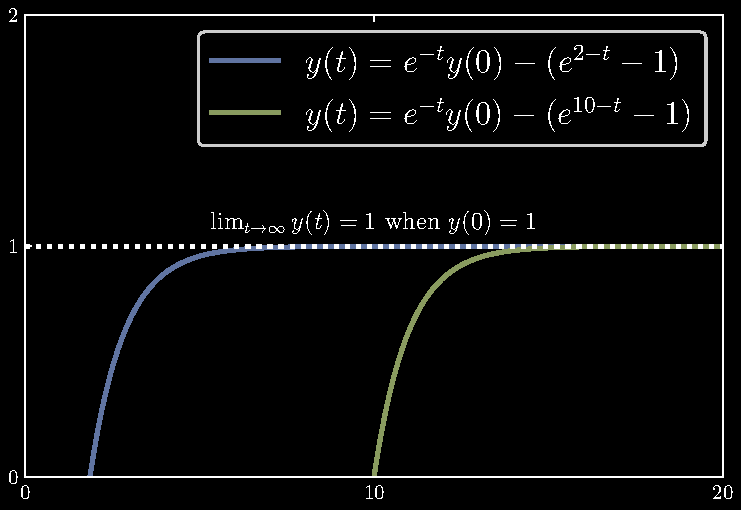
\includegraphics[width=1.0\textwidth]{../chap1/sec1.4/chap1sec1.4ex14.eps}
\end{center}

% QUESTION 15
\qs{1.4.15}{Draw the ramp function that solves \(y' = H \!\left( t - T \right) \) with \(y \!\left( 0 \right) = 2\).}

We solve the equation by:

\begin{alignat*}{3}
	&\implies && \int^{t}_{0} \frac{d y}{d t}  \ dt && = \int^{t}_{T} H \!\left( t - T \right)  \ dt   \\
	&\implies && y \!\left( t \right) - y \!\left( 0 \right) && = R \!\left( t - T \right)  \\
	&\implies && y \!\left( t \right) && = 2 + R \!\left( t - T \right) 
\end{alignat*}

where we define \(R \!\left( t - T \right) \) as
\[
	R \!\left( t - T \right) = \begin{cases}
		t - T & t \ge T \\
		0 & t < T \\
	\end{cases}
\]

For \(T = 3\), we graph the solution as

\begin{center}
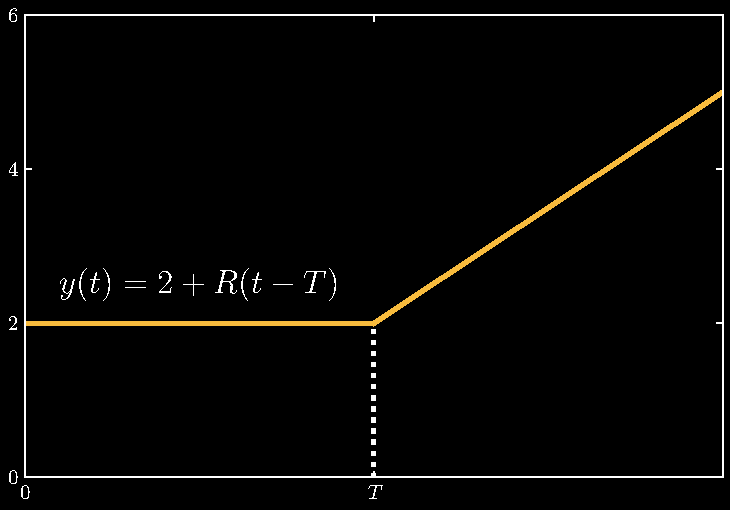
\includegraphics[width=1.0\textwidth]{../chap1/sec1.4/chap1sec1.4ex15.eps}
\end{center}

% QUESTION 16
\qs{1.4.16}{Find \(y_{n} \!\left( t \right) \) and \(y_{p} \!\left( t \right) \) as in equation (10), with step function inputs starting at \(T = 4\).

\begin{enumerate}[label=(\alph*)]
	\item \(y' - 5y = 3H \!\left( t - 4 \right) \)
	\item \(y' + y = 7H \!\left( t - 4 \right) \)
\end{enumerate}

(\textit{What is \(y_{\infty}\)?})}

(a) Our integrating factor is \(e^{-5t}\). Solving the equation yields:

\begin{alignat*}{3}
	&\implies && \!\left( e^{-5t}y \right)' && = 3e^{-5t} H \!\left( t - 4 \right)  \\
	&\implies && e^{-5t} y \!\left( t \right) - y \!\left( 0 \right) && = \int^{t}_{4} 3e^{-5s} \ ds  \\
	& && && = -\frac{3}{5} \!\left( e^{-5t} - e^{-20} \right) \\
	&\implies && y \!\left( t \right) && = \underbrace{e^{5t} y \!\left( 0 \right)}_{y_{n} \!\left( t \right) } + \underbrace{\frac{3}{5} \!\left( e^{5 \!\left(t - 4 \right) } - 1 \right)}_{y_{p} \!\left( t \right) }
\end{alignat*}

Here, the asymptotic behavior of \(y \!\left( t \right) \) appears to diverge:
\[
	\lim\limits_{t \to \infty} y \!\left( t \right) = +\infty
\]

which we expect since the growth rate, \(a = 5\), is positive.

\begin{center}
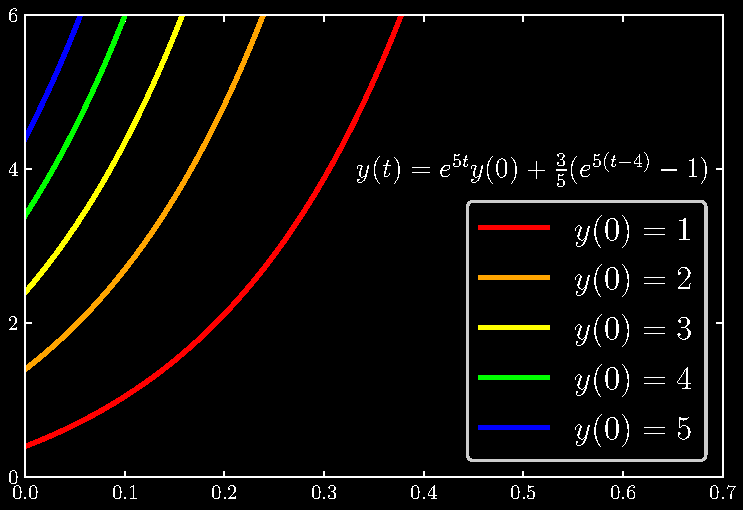
\includegraphics[width=1.0\textwidth]{../chap1/sec1.4/chap1sec1.4ex16a.eps}
\end{center}

\vspace{12pt}

(b) Next, our integrating factor is \(e^{t}\):

\begin{alignat*}{3}
	&\implies && \!\left( e^{t}y \right)' && = 7 e^{t} H \!\left( t - 4 \right)  \\
	&\implies && e^{t} y \!\left( t \right) - y \!\left( 0 \right) && = \int^{t}_{4} 7e^{s} \ ds  \\
	& && && = 7 \!\left( e^{t} - e^{4} \right) \\
	&\implies && y \!\left( t \right) && = \underbrace{e^{-t} y \!\left( 0 \right)}_{y_{n} \!\left( t \right) } \underbrace{- 7 \!\left( e^{- \!\left( t - 4 \right) } - 1 \right)}_{y_{p} \!\left( t \right) }
\end{alignat*}

with limiting behavior
\[
	\lim\limits_{t \to \infty} y \!\left( t \right) = 7
\]

\begin{center}
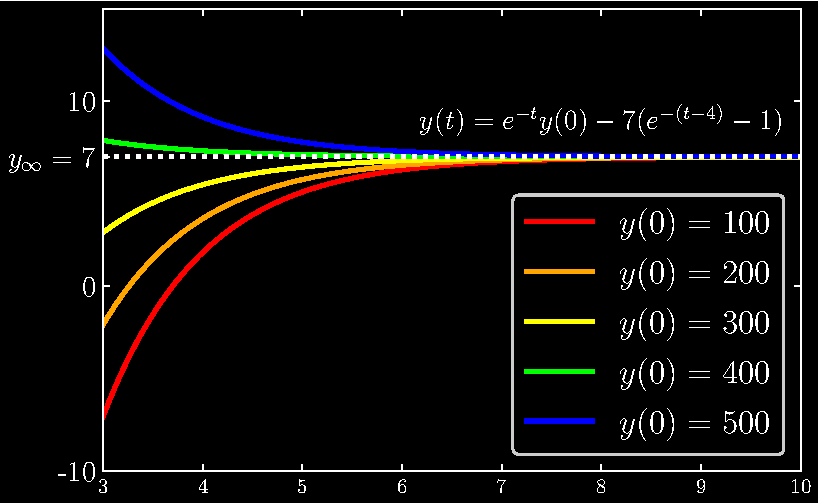
\includegraphics[width=1.0\textwidth]{../chap1/sec1.4/chap1sec1.4ex16b.eps}
\end{center}

% QUESTION 17
\qs{1.4.17}{Suppose the step function turns on at \(T = 4\) and off at \(T = 6\). Then \(q \!\left( t \right) = H \!\left( t - 4 \right) - H \!\left( t - 6 \right) \). Starting from \(y \!\left( 0 \right) = 0\), solve \(y' + 2y = q \!\left( t \right) \). What is \(y_{\infty}\)?}

With integrating factor \(e^{2t}\), we derive:

\begin{alignat*}{3}
	&\implies && \!\left( e^{2t} y \right)' && = e^{2t} \left[ H \!\left( t-4 \right) - H \!\left( t-6 \right)  \right]  \\
	&\implies && e^{2t} y \!\left( t \right) && = \int^{t}_{4} e^{2s} \ ds - \int^{t}_{6} e^{2s} \ ds   \\ 
	& && && = \begin{cases}
		0 & 0 \le t < 4 \\
		\frac{1}{2} \!\left( e^{2t} - e^{8} \right) & 4 \le t < 6 \\
		\frac{1}{2} \!\left( e^{2t} - e^{8} \right) - \frac{1}{2} \!\left( e^{2t} - e^{12} \right) & 6 \le t 
	\end{cases}\\
	& && && = \begin{cases}
		0 & 0 \le t < 4 \\
		\frac{1}{2} \!\left( e^{2t} - e^{8} \right) & 4 \le t < 6 \\
		\frac{1}{2} \!\left( e^{12} - e^{8} \right) & 6 \le t 
	\end{cases} \\
	&\implies && y \!\left( t \right) && = \begin{cases}
		0 & 0 \le t < 4 \\
		-\frac{1}{2} \!\left( e^{-2 \!\left( t - 4 \right) } - 1\right) & 4 \le t < 6 \\
		-\frac{1}{2} \!\left( e^{-2 \!\left( t - 4 \right) }  - e^{-2 \!\left( t-6 \right) } \right) & 6 \le t
	\end{cases}
\end{alignat*}

More concisely, we may also write:
\[
	y \!\left( t \right) = \frac{1}{2} \left[ - \!\left( e^{-2 \!\left( t - 4 \right) } - 1 \right) H \!\left( t - 4 \right) + \!\left( e^{-2 \!\left( t - 6 \right) } - 1 \right) H \!\left( t - 6 \right)  \right] 
\]
Implying that
\[
	\lim\limits_{t \to \infty} y \!\left( t \right) = 0
\]

\begin{center}
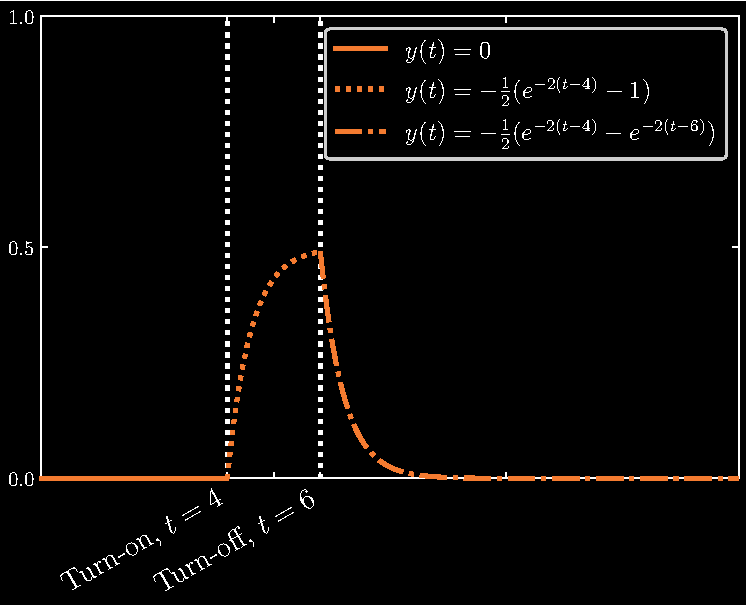
\includegraphics[width=1.0\textwidth]{../chap1/sec1.4/chap1sec1.4ex17.eps}
\end{center}

% QUESTION 18
\qs{1.4.18}{Suppose \(y' = H \!\left( t-1 \right) + H \!\left( t-2 \right) + H \!\left( t-3 \right) \), starting at \(y \!\left( 0 \right) = 0\). Find \(y \!\left( t \right) \).}

Integrating yields
\[
	y = R \!\left( t - 1 \right) + R \!\left( t - 2 \right) + R \!\left( t - 3 \right) 
\]
but we may simplify this result further. Recall that the definition of our ramp function \(R \!\left( t - T\right) \) is
\[
	R \!\left( t - T \right) = \begin{cases}
		t - T & t \ge T \\
		0 & t < T \\
	\end{cases}
\]
Applying this to the constituent ramp functions of \(y \!\left( t \right) \), we can derive
\[
	y \!\left( t \right) = \begin{cases}
		0 & 0 \le t < 1 \\
		t - 1 & 1 \le t < 2 \\
		2t - 3 & 2 \le t < 3 \\
		3 \!\left( t - 2 \right) & 3 \ge t
	\end{cases}
\]
which alternatively can be written as
\[
	y \!\left( t \right) = \!\left( t - 1 \right) H \!\left( t - 1 \right) + \!\left( t - 2 \right) H \!\left( t - 2 \right) + \!\left( t - 3 \right) H \!\left( t - 3 \right) 
\]
Graphing the function, we can visually see what is happening here: as we turn on more and more switches (at times \(t = 1, 2, 3\) to more and more sources, the growth of \(y \!\left( t \right) \) happens at a steeper and steeper rate.

\begin{center}
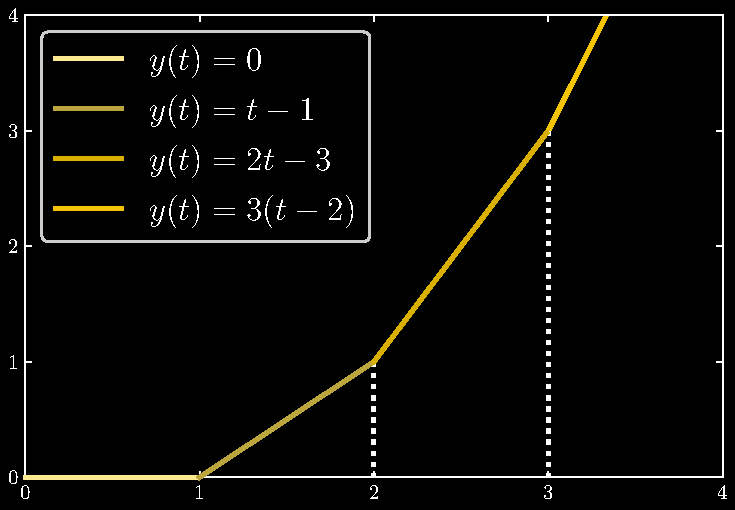
\includegraphics[width=1.0\textwidth]{../chap1/sec1.4/chap1sec1.4ex18.eps}
\end{center}

% QUESTION 19
\qs{1.4.19}{For all \(t > 0\) find these integrals \(a \!\left( t \right) , b \!\left( t \right), c \!\left( t \right) \) of point sources and graph \(b \!\left( t \right) \):
\begin{enumerate}[label=(\alph*)]
	\item \( {\displaystyle \int^{t}_{0} \delta \!\left( T - 2 \right) \, dT} \)
	\item \({\displaystyle \int^{t}_{0} \!\left( \delta \!\left( T - 2 \right) - \delta \!\left( T - 3 \right) \right)  \, dT} \)
	\item \( {\displaystyle \int^{t}_{0} \delta \!\left( T - 2 \right) \delta \!\left( T - 3 \right)  \, dT} \)
\end{enumerate}}

(a) If \(t \ge 2\), it will be the case that the domain of integration includes the point \(T = 2\). Ergo, we have
\[
	a \!\left( t \right) = \int^{t}_{0} \delta \!\left( T - 2 \right)  \, dT = H \!\left( T - 2 \right) = \begin{cases}
		0 & t < 2 \\
		1 & t \ge 2 \\
	\end{cases}
\]
Graphically, we have
\begin{center}
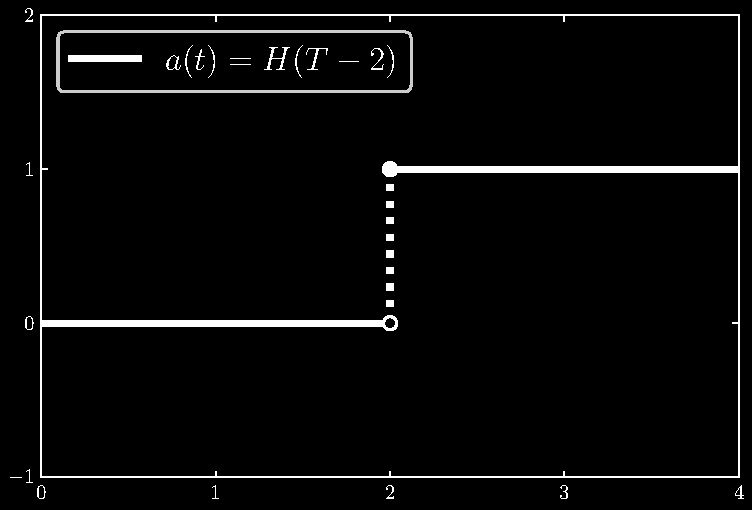
\includegraphics[width=1.0\textwidth]{../chap1/sec1.4/chap1sec1.4ex19a.eps}
\end{center}
(b) We rewrite \(b \!\left( t \right) \) as
\[
	b \!\left( t \right) = \int^{t}_{0} \!\left( \delta \!\left( T - 2 \right) - \delta \!\left( T - 3 \right)  \right)  \, dT = \int^{t}_{0} \delta \!\left( T - 2 \right)  \, dT - \int^{t}_{0} \delta \!\left( T - 3 \right)  \, dT   
\]
Now, the value of each term is contingent on our choice of \(t\). For \(t < 2\), each term vanishes. For \(2 \le t < 3\), the first term is 1, while the second term vanishes. Lastly, for \(t \ge 3\), both terms are 1, and the difference vanishes. Succinctly, put, we have 
\[
	\int^{t}_{0} \delta \!\left( T-2 \right)  \, dT = H \!\left( T-2 \right) \qquad \text{and} \qquad \int^{t}_{0} \delta \!\left( T-3 \right)  \, dT = H \!\left( T-3 \right)   
\]
and solve as
\[
	b \!\left( t \right) = \int^{t}_{0} \!\left( \delta \!\left( T - 2 \right) - \delta \!\left( T - 3 \right)  \right)  \, dT = \begin{cases}
		1 & 2 \le t < 3 \\
		0 & \text{otherwise} \\
	\end{cases} 
\]

Intuitively, we can interpret this as at time \(T = 2\), we ``deposit" an impulse, and at time \(T = 3\), we ``withdraw" the impulse, leaving us with nothing once more. Graphically, we represent \(b \!\left( t \right) \) as

\begin{center}
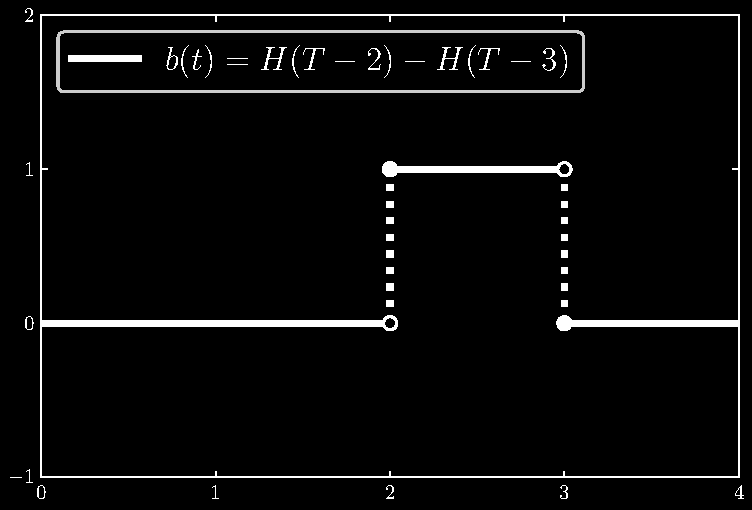
\includegraphics[width=1.0\textwidth]{../chap1/sec1.4/chap1sec1.4ex19bi.eps}
\end{center}

along with the integrand

\begin{center}
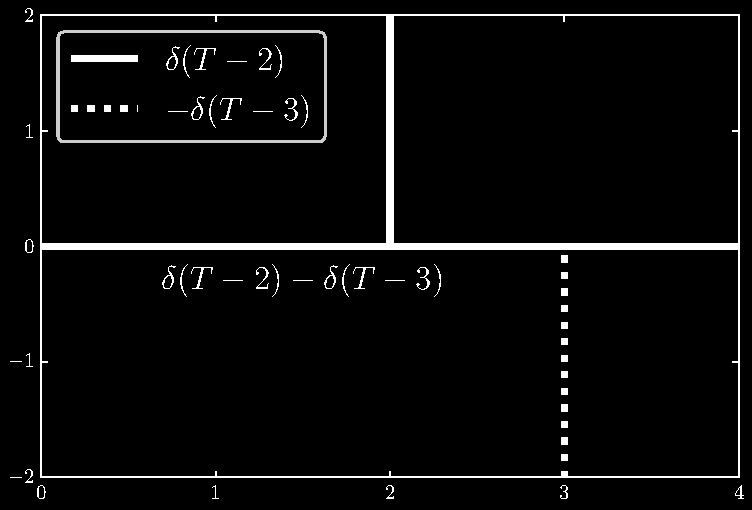
\includegraphics[width=1.0\textwidth]{../chap1/sec1.4/chap1sec1.4ex19b.eps}
\end{center}

(c) Observe that irrespective of our choice of \(t\), it cannot ever be the case that the product \(\delta \!\left( T - 2 \right) \delta \!\left( T - 3 \right) \) is equal to anything other than zero. For when either constituent of the product is non-zero, it must be the case that the other is zero. Conceptually, we may have an impulse at one time for one of the delta functions, but that means there cannot be an impulse in the other delta function. Hence,
\[
	c \!\left( t \right) = \int^{t}_{0} \delta \!\left( T - 2 \right) \delta \!\left( T - 3 \right)  \, dT = 0 \text{ for all } t 
\]

% QUESTION 20
\qs{1.4.20}{Why are all these answers reasonable? (They are all correct.)
\begin{enumerate}[label=(\alph*)]
	\item \( \displaystyle \int^{\infty}_{-\infty} e^{t} \delta \!\left( t \right)  \, dt = 1\)
	\item \( \displaystyle \int^{\infty}_{-\infty} \!\left( \delta \!\left( t \right)  \right)^{2}  \, dt = \infty \)
	\item \( \displaystyle \int^{\infty}_{-\infty} e^{T}\delta \!\left( t - T \right)  \, dT = e^{t} \)
\end{enumerate}}

(a) Recall that
\[
	\int^{\infty}_{-\infty} \delta \!\left( t \right) F \!\left( t \right)  \, dt = F \!\left( 0 \right)  
\]
Therefore, we have \(F \!\left( t \right) = e^{t}\), thus
\[
	\int^{\infty}_{-\infty} e^{t} \delta \!\left( t \right)  \, dt = e^{0} = 1
\]

(b) Again invoking the aforementioned identity, we have \(F \!\left( t \right) = \delta \!\left( t \right) \), giving us
\[
	\int^{\infty}_{-\infty} \!\left( \delta \!\left( t \right)  \right)^{2} \, dt = \delta \!\left( 0 \right) = \infty 
\]

(c) Here we recall the identity
\[
	\int^{\infty}_{-\infty} \delta \!\left( t - T \right) F \!\left( t \right)  \, dt = F \!\left( T \right)  
\]
In the given integral equation, however, the variable of integration is \(T\). What matters is the value that \(F \!\left( T \right) = e^{T}\) takes is time \(T\) at which \(\delta \!\left( t - T \right) \) has argument zero. This is precisely when \(T = t\), hence
\[
	\int^{\infty}_{-\infty} e^{T} \delta \!\left( t - T \right)  \, dT = e^{t}
\]

% QUESTION 21
\qs{1.4.21}{\textit{The solution to} \(y' = 2y + \delta \!\left( t - 3 \right) \) \textit{jumps up by } \(1\) \textit{at} \(t = 3\). Before and after \(t = 3\), the delta function is zero and \(y\) grows like \(e^{2t}\). Draw the graph of \(y \!\left( t \right) \) when
\begin{enumerate}[label=(\alph*)]
	\item \( y \!\left( 0 \right) = 0 \) and
	\item \(y \!\left( 0 \right) = 1\).
\end{enumerate}
Write formulas for \(y \!\left( t \right) \) before and after \(t = 3\).}

We solve the differential equation with integrating factor \(e^{-2t}\) as follows:

\begin{alignat*}{3}
	&\implies && y' - 2y && = \delta \!\left( t - 3 \right)  \\
	&\implies && \!\left( e^{-2t}y \right)' && = e^{-2t} \delta \!\left( t - 3 \right)  \\
	&\implies && e^{-2t}y \!\left( t \right) - y \!\left( 0 \right) && = \int^{t}_{0} e^{-2s} \delta \!\left( s-3 \right)  \, ds \\
	& && && = \begin{cases}
		0 & 0 \le t < 3 \\
		\displaystyle{e^{-6}} & t \ge 3 
		\end{cases} \\
	&\implies && y \!\left( t \right) && = \begin{cases}
		e^{2t} y \!\left( 0 \right)  & 0 \le t < 3 \\
		\displaystyle{e^{2t} y \!\left( 0 \right) + e^{2 \!\left( t - 3 \right) }} & t \ge 3 
		\end{cases} \\
										       & && && = e^{2t} y \!\left( 0 \right) + H \!\left( t - 3 \right) e^{2 \!\left( t - 3 \right) }
\end{alignat*}

In the case of (a), we have
\[
	y \!\left( t \right) = H \!\left( t - 3 \right) e^{2 \!\left( t-3 \right) }
\]
and for (b)
\[
	y \!\left( t \right) = e^{2t} + H \!\left( t - 3 \right) e^{2 \!\left( t - 3 \right) }
\]
which has graph
\begin{center}
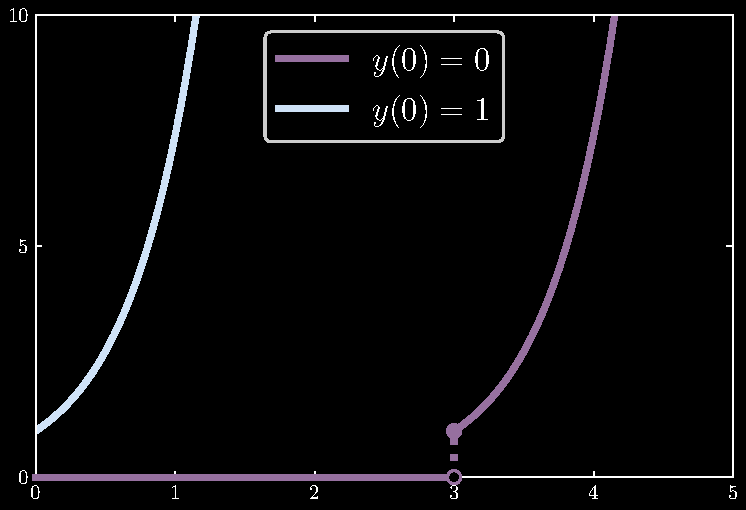
\includegraphics[width=1.0\textwidth]{../chap1/sec1.4/chap1sec1.4ex21.eps}
\end{center}

% QUESTION 22
\qs{1.4.22}{Solve these differential equations starting at \(y \!\left( 0 \right) = 2\):
\begin{enumerate}[label=(\alph*)]
	\item \(y' - y = \delta \!\left( t - 2 \right) \)
	\item \(y' + y = \delta \!\left( t - 2 \right) \)
\end{enumerate}
(\textit{What is \(y_{\infty}\)}?)}

(a) Beginning with integrating factor \(e^{-t}\), we have
\begin{alignat*}{3}
	&\implies && \!\left( e^{-t} y \right)' && = e^{-t} \delta \!\left( t - 2 \right)  \\
	&\implies && e^{-t} y \!\left( t \right) - y \!\left( 0 \right) && = \int^{t}_{0} e^{-s} \delta \!\left( s-2 \right)  \, ds  \\
	& && && = \begin{cases}
		0 & 0 \le t < 2 \\
		e^{-2} & t \ge 2 \\
	\end{cases} \\
	&\implies && y \!\left( t \right) && = e^{t} y \!\left( 0 \right) + H \!\left( t - 2 \right) e^{t-2} \\
	& && && = 2e^{t} + H \!\left( t - 2 \right) e^{t-2}
\end{alignat*}
It follows that
\[
	\lim\limits_{t \to \infty} y \!\left( t \right) = +\infty
\]
(b) Now, with integrating factor \(e^{t}\), we have
\begin{alignat*}{3}
	&\implies && \!\left( e^{t}y \right)' && = e^{t} \delta \!\left( t-2 \right)  \\
	&\implies && e^{t} y \!\left( t \right) - y \!\left( 0 \right) && = \int^{t}_{0} e^{s} \delta \!\left( s - 2 \right)  \, ds  \\ 
	& && && = \begin{cases}
		0 & 0 \le t < 2 \\
		e^{2} & t \ge 2 \\
	\end{cases} \\
	&\implies && y \!\left( t \right) && = e^{-t} y \!\left( 0 \right) + H \!\left( t-2 \right) e^{-\!\left( t-2 \right) } \\
	& && && = 2 e^{-t} + H \!\left( t - 2 \right) e^{-\!\left( t-2 \right) }
\end{alignat*}
which has limiting behavior
\[
	\lim\limits_{t \to \infty} = 0
\]

Intuitively, in the case of (b), we have an instantaneous impulse at time \(t=2\), after which we have a decay.

\begin{center}
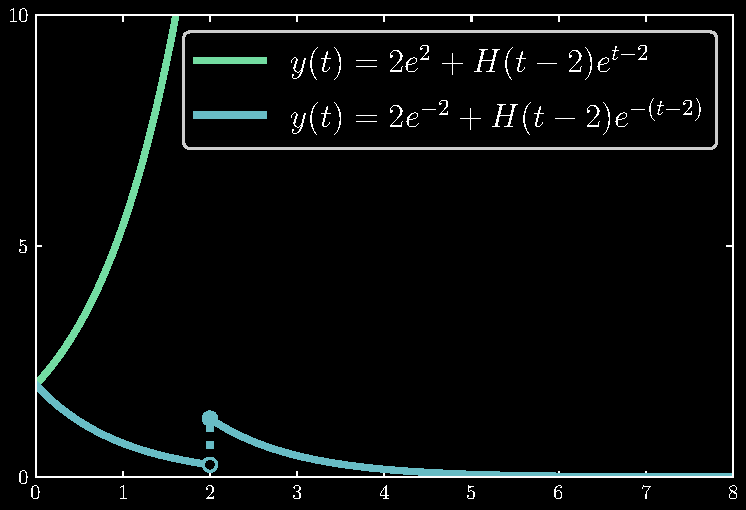
\includegraphics[width=1.0\textwidth]{../chap1/sec1.4/chap1sec1.4ex22.eps}
\end{center}

% QUESTION 23
\qs{1.4.23}{Solve \(dy/dt = H \!\left( t-1 \right) + \delta \!\left( t-1 \right) \) starting from \(y \!\left( 0 \right) = 0\): jump and ramp.}

Solving as follows, we find
\begin{alignat*}{3}
	&\implies && y \!\left( t \right) - y \!\left( 0 \right) && = \int^{t}_{0} H \!\left( s-1 \right)  \, ds + \int^{t}_{0} \delta \!\left( s-1 \right)  \, ds   \\
	&\implies && y \!\left( t \right) && = R \!\left( t-1 \right) + H \!\left( t - 1 \right)   \\
	& && && = \begin{cases}
		0 & t < 1 \\
		t & t \ge 1 \\
	\end{cases}
\end{alignat*}

Intuitively, at time \(t=1\), we have an impulse which causes a jump to \(y \!\left( 1 \right) = 1\), after which we have constant growth through the ramp function.
\begin{center}
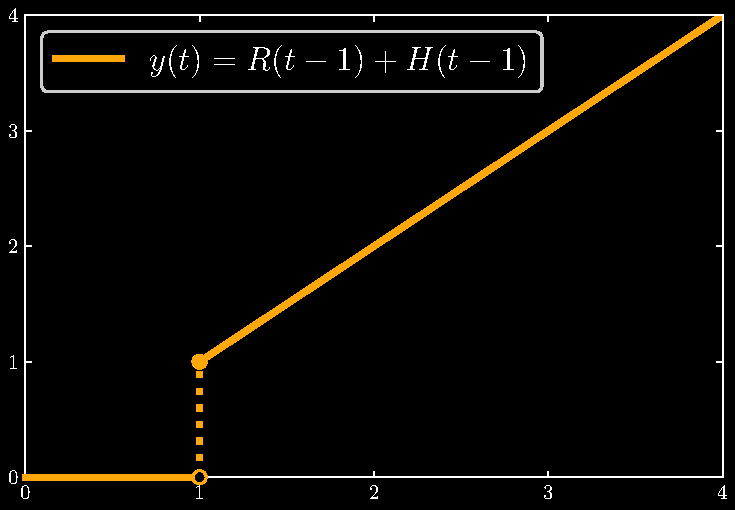
\includegraphics[width=1.0\textwidth]{../chap1/sec1.4/chap1sec1.4ex23.eps}
\end{center}

% QUESTION 24
\qs{1.4.24}{(My small favorite) What is the steady state \(y_{\infty}\) for \(y' = -y + \delta \!\left( t-1 \right) + H 
\!\left( t-3 \right) \)?}
Using integrating factor \(e^{t}\), we find
\begin{alignat*}{3}
	&\implies && y' + y && = \delta \!\left( t-1 \right) + H \!\left( t-3 \right)  \\
	&\implies && \!\left( e^{t}y \right)' && = e^{t} \delta \!\left( t-1 \right) + e^{t} H \!\left( t-3 \right)  \\ 
	&\implies && e^{t} y \!\left( t \right) - y \!\left( 0 \right) && = \int^{t}_{0} e^{s} \delta \!\left( s-1 \right)  \, ds + \int^{t}_{0} e^{s} H \!\left( s-3 \right)  \, ds \\
	& && && = e H \!\left( t-1 \right) + e^{t} H \!\left( t-3 \right) \\
	&\implies && y \!\left( t \right) && = e^{-t} y \!\left( 0 \right) + e^{-\!\left( t-1 \right) } H \!\left( t-1 \right) + H \!\left( t-3 \right) 
\end{alignat*}
which features limiting behavior
\[
	\lim\limits_{t \to \infty} y \!\left( t \right) = 1
\]
Thus our steady state is \(y_{\infty} = 1\).

\vspace{12pt}

% QUESTION 25
\qs{1.4.25}{Which \(q\) and \(y \!\left( 0 \right) \) in \(y' - 3y = q \!\left( t \right) \) produce the step solution \(y \!\left( t \right) = H \!\left( t-1 \right) \)?}

Given \(y \!\left( t \right) = H \!\left( t-1 \right) \), we must have \(y \!\left( 0 \right) = 0\). Moreover, it follows that \(y'\!\left( t \right) = \delta \!\left( t-1 \right) \). Thus \(q \!\left( t \right) \) must be
\[
	q \!\left( t \right) = \delta \!\left( t-1 \right) - 3 H \!\left( t-1 \right) 
\]
Graphically, the source \(q \!\left( t \right) \) appears as
\begin{center}
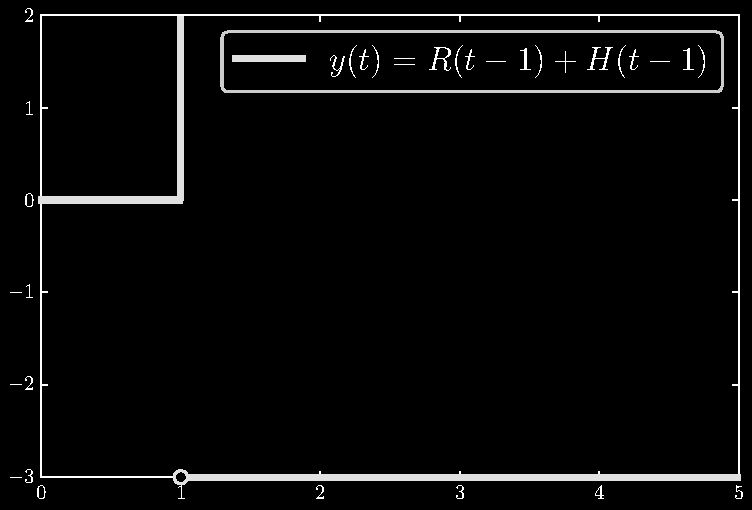
\includegraphics[width=1.0\textwidth]{../chap1/sec1.4/chap1sec1.4ex25.eps}
\end{center}

% QUESTION 26
\qs{1.4.26}{Solve these equations \(y' - ay = Qe^{ct}\) as in (19), starting from \(y \!\left( 0 \right) = 2\):
\begin{enumerate}[label=(\alph*)]
	\item \(y' - y = 8e^{3t}\)
	\item \(y' + y = 8e^{-3t}\)
\end{enumerate}
(\textit{What is} \(y_{\infty}\)?)}

(a) Let \(y_{p} = 8Ye^{3t}\). Then \(y_{p}' = 24Ye^{3t}\) and we have, substituting \(y_{p}\) for \(y\):
\begin{alignat*}{3}
	&\implies && 24Ye^{3t} - 8Ye^{3t} && = 8e^{3t} \\
	&\implies && 3Y - Y && = 1 \\ 
	&\implies && Y && = 1/2
\end{alignat*}
Thus we have that \(y_{p} = 4e^{3t}\), where the particular solution starts at \(y_{p} \!\left( 0 \right) = 4\). The null solution must start at \(-2\), and is given by
\[
	y_{n} = -2e^{t}
\]
And the complete solution is
\[
	y \!\left( t \right) = \underbrace{-2e^{t}}_{y_{n}} + \underbrace{4e^{3t}}_{y_{p}}
\]
with limiting behavior
\[
	\lim\limits_{t \to \infty} y \!\left( t \right) = +\infty
\]
(b) Let \(y_{p} = 8Ye^{-3t}\). Then \(y_{p}' = -24Ye^{-3t}\) and we have, substituting \(y_{p}\) for \(y\):
\begin{alignat*}{3}
	&\implies && -24Ye^{-3t} + 8Ye^{-3t} && = 8e^{-3t} \\
	&\implies && -3Y + Y && = 1 \\
	&\implies && Y && = -1/2
\end{alignat*}
So we must have \(y_{p} = -4e^{-3t}\). As our particular solution begins at \(y_{p} \!\left( 0 \right) = -4\), our null solution must commence at 6, giving us
\[
	y_{n} = 6e^{-t}
\]
Thus we have complete solution
\[
	y \!\left( t \right) = \underbrace{6e^{-t}}_{y_{n}} \underbrace{-4e^{-3t}}_{y_{p}}
\]
with limiting behavior
\[
	\lim\limits_{t \to \infty} y \!\left( t \right) = 0
\]
\begin{center}
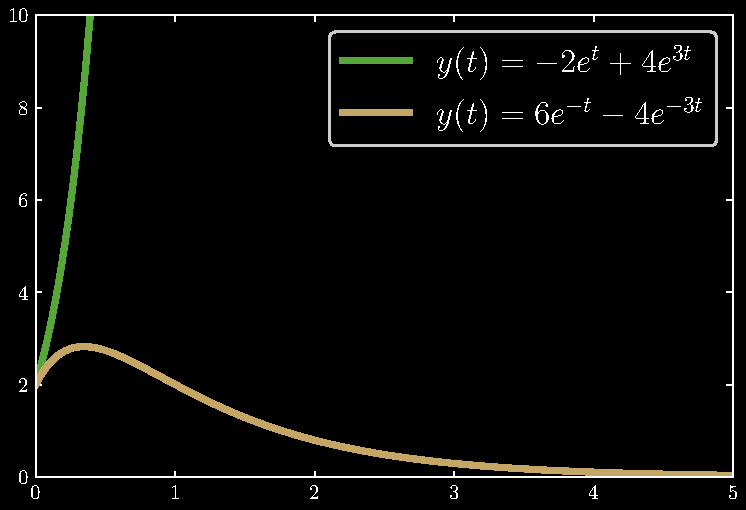
\includegraphics[width=1.0\textwidth]{../chap1/sec1.4/chap1sec1.4ex26.eps}
\end{center}

% QUESTION 27
\qs{1.4.27}{When \(c = 2.01\) is very close to \(a = 2\), solve \(y' - 2y = e^{ct}\) starting from \(y \!\left( 0 \right) = 1\). This is resonance as in equation (20). By hand or computer, draw the graph of \(y \!\left( t \right) \).}

Let \(y_{p} = Ye^{ct}\). Then \(y_{p}' = cYe^{ct}\), and substituting, we find
\begin{alignat*}{3}
	&\implies && cYe^{ct} - 2Ye^{ct} && = e^{ct} \\
	&\implies && cY - 2Y = 1 \\ 
	&\implies && Y = \frac{1}{c - 2}
\end{alignat*}
Thus
\[
	y_{p} = \frac{e^{ct}}{c - 2}
\]
which starts at \(y_{p} \!\left( 0 \right) = \displaystyle{\frac{1}{c-2}}\). Then \(y_{n}\) must begin at \(\displaystyle{\frac{c - 3}{c - 2}}\), giving us
\[
	y_{n} = \frac{c-3}{c-2} e^{2t}
\]
and finally, the complete solution
\[
	y \!\left( t \right) = \underbrace{\frac{c-3}{c-2} e^{2t}}_{y_{n}} + \underbrace{\frac{1}{c-2} e^{ct}}_{y_{p}}
\]
For \(c = 2.01\), we evaluate \(y \!\left( t \right) \) as
\[
	y \!\left( t \right) = \underbrace{-99e^{2t}}_{y_{n}} + \underbrace{100e^{2.01t}}_{y_{p}}
\]
Cycling through values of \(c\) as we approach 2, we can graph the following trajectories:
\begin{center}
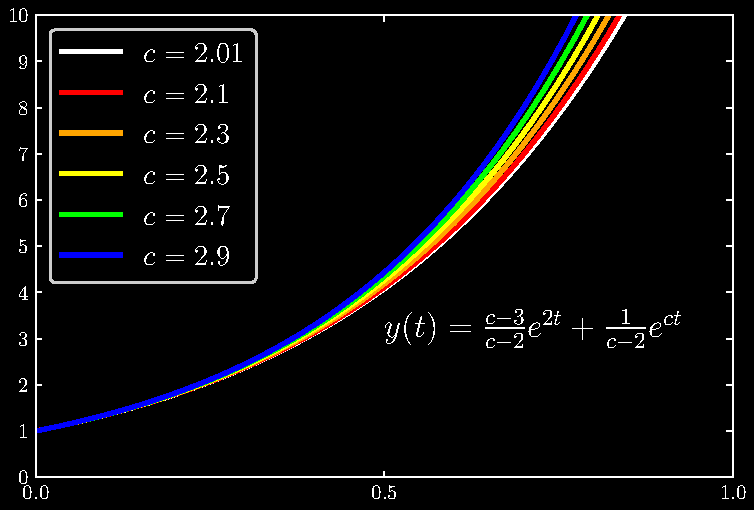
\includegraphics[width=1.0\textwidth]{../chap1/sec1.4/chap1sec1.4ex27.eps}
\end{center}

% QUESTION 28
\qs{1.4.28}{When \(c = 2\) is exactly equal to \(a = 2\), solve \(y' - 2y = e^{2t}\) starting from \(y \!\left( 0 \right) = 1\). This resonance is as in equation (20). By hand or computer, draw the graph of \(y \!\left( t \right) \).}

Using the integrating factor \(e^{-2t}\), write
\begin{alignat*}{3}
	&\implies && \!\left( e^{-2t}y \right)' && = 1 \\
	&\implies && e^{-2t}y \!\left( t \right) - y \!\left( 0 \right) && = \int^{t}_{0} \, ds  \\ 
	&\implies && y \!\left( t \right) && = \underbrace{e^{2t}}_{y_{n}} + \underbrace{te^{2t}}_{y_{p}}
\end{alignat*}

We graphically represent \(y \!\left( t \right) \) as:
\begin{center}
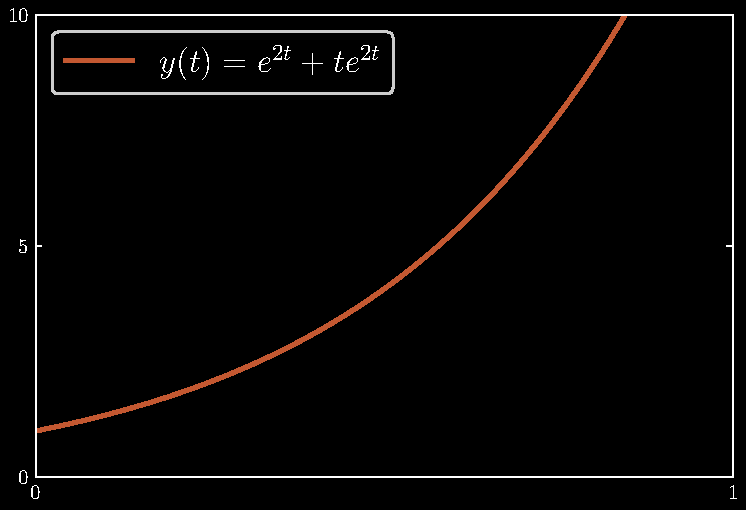
\includegraphics[width=1.0\textwidth]{../chap1/sec1.4/chap1sec1.4ex28.eps}
\end{center}

% QUESTION 29
\qs{1.4.29}{Solve \(y' + 4y = 8e^{-4t} + 20\) starting from \(y \!\left( 0 \right) = 0\). What is \(y_{\infty}\)?}

Using integrating factor \(e^{4t}\), we have
\begin{alignat*}{3}
	&\implies && \!\left( e^{4t}y \right)' && = 8 + 20e^{4t}\\
	&\implies && e^{4t} y \!\left( t \right) - y \!\left( 0 \right) && = \int^{t}_{0} 8 \, ds + \int^{t}_{0} 20e^{4s} \, ds   \\
	&\implies && y \!\left( t \right) && = e^{-4t} y \!\left( 0 \right) + 8te^{-4t} - 5e^{-4t} + 5 \\
	& && && = 5 - 5e^{-4t} + 8te^{-4t}
\end{alignat*}

which has limiting behavior
\[
	\lim\limits_{t \to \infty} y \!\left( t \right) = 5
\]

% QUESTION 30
\qs{1.4.30}{The solution to \(y' - ay = e^{ct}\) didn't come from the main formula (4), but it could. Integrate \(e^{-as}e^{cs}\) in (4) to reach the very particular solution \(\!\left( e^{ct} - e^{at} \right) / \!\left( c - a \right) \).}

Using the integrating factor \(e^{-at}\), derive
\begin{alignat*}{3}
	&\implies && \!\left( e^{-at}y \right)' && = e^{-at} e^{ct} \\
	&\implies && e^{-at} y \!\left( t \right) - y \!\left( 0 \right) && = \int^{t}_{0} e^{\!\left( c - a \right) s} \, ds   \\ 
	& && && = \frac{e^{\!\left( c - a \right) t} - 1}{c - a} \\
	&\implies && y \!\left( t \right) && = e^{at} y \!\left( 0 \right) + \frac{e^{ct} - e^{at}}{c - a}
\end{alignat*}
where the second term is the very particular solution.

% QUESTION 31
\qs{1.4.31}{\textit{The easiest possible equation} \(y' = 1\) \textit{has resonance}! The solution \(y = t\) shows the factor \(t\). What number is the growth rate \(a\) and also the exponent \(c\) in the source?}

Here, we have \(a = c = 0\); it is clear that \(y' - ay = e^{ct}\) reduces to \(y' = 1\) with the aforementioned values.

\vspace{12pt}

% QUESTION 32
\qs{1.4.32}{Suppose you know two solutions \(y_{1}\) and \(y_{2}\) to the equation \(y' - a \!\left( t \right) y = q \!\left( t \right) \).
\begin{enumerate}[label=(\alph*)]
	\item Find a null solution to \(y' - a \!\left( t \right) y = 0\).
	\item Find all null solutions \(y_{n}\). Find all particular solutions \(y_{p}\).
\end{enumerate}}

(a) By premise, \(y_{1}\) and \(y_{2}\) solve the differential equation, meaning
\[
	y_{1}' - a \!\left( t \right) y_{1} = q \!\left( t \right) \qquad \text{and} \qquad y_{2}' - a \!\left( t \right) y_{2} = q \!\left( t \right) 
\]
In appealing to linearity, we can immediately deduce that the differences of the solutions, \(y_{1} - y_{2}\) and \(y_{2} - y_{1}\), are both null solutions:
\[
	\!\left( y_{1} - y_{2} \right)' - a \!\left( t \right) \!\left( y_{1} - y_{2} \right) = 0 \qquad \text{and} \qquad \!\left( y_{2} - y_{1} \right)' - a \!\left( t \right) \!\left( y_{2} - y_{1} \right) = 0
\]
(b) Once again appealing to linearity, all null solutions include solutions of the form \(\alpha \!\left( y_{1} - y_{2} \right)\) for all \(\alpha \in \mathbb{R}\). Moreover, observe that if we have \(\alpha y_{1}\) and \(\beta y_{2}\), we have
\[
	\alpha \!\left( y_{1}' - a \!\left( t \right) y_{1}\right) = \alpha q \!\left( t \right) \qquad \text{and} \qquad \beta \!\left( y_{2}' - a \!\left( t \right) y_{2} \right) = \beta q \!\left( t \right)  
\]
Then for any nonzero sum \(\alpha + \beta \), \(\alpha, \beta \in \mathbb{R}\), we have a ``weighted average" \textbf{linear combination} of particular solutions:
\[
	\frac{\alpha }{\alpha + \beta } y_{1} + \frac{\beta }{\alpha + \beta } y_{2}
\]

% QUESTION 33
\qs{1.4.33}{Turn back to the first page of this Section 1.4. Without looking, can you write down a solution to \(y' - ay = q \!\left( t \right) \) for all four source functions \(\bm{q }, \bm{H \!\left( t \right) }, \bm{\delta \!\left( t \right) }, \bm{e^{ct}}\)?}

For simplicity, assume \(y \!\left( 0 \right) = 0\).

\(\bm{q}:\) \(y' - ay = q\)

Using integrating factor \(e^{-at}\), calculate
\begin{alignat*}{3}
	&\implies && \!\left( e^{-at}y \right)' && = e^{-at} q  \\
	&\implies && e^{-at} y \!\left( t \right) && = \int^{t}_{0} e^{-as}q  \, ds   \\ 
	& && && = -\frac{q }{a} \!\left( e^{-at} - 1 \right) \\ 
	&\implies && y \!\left( t \right) && = -\frac{q }{a} \!\left( 1 - e^{at} \right) \\
	& && && = \boxed{\frac{q }{a} \!\left( e^{at} - 1 \right) }
\end{alignat*}

\(\bm{H \!\left( t \right) }\): \(y' - ay = H \!\left( t \right) \)

Using integrating factor \(e^{-at}\), calculate
\begin{alignat*}{3}
	&\implies && \!\left( e^{-at}y \right)' && = e^{-at} H \!\left( t \right)   \\
	&\implies && e^{-at} y \!\left( t \right) && = \int^{t}_{0} e^{-as} H \!\left( s \right)  \, ds  \\ 
	& && && = -\frac{1}{a} \!\left( e^{-at} - 1 \right) \\
	&\implies && y \!\left( t \right) && = \boxed{ \frac{1}{a} \!\left( e^{at} - 1 \right) }
\end{alignat*}

\(\bm{\delta \!\left( t \right) }\): \(y' - ay = \delta \!\left( t \right) \)

Using integrating factor \(e^{-at}\), calculate
\begin{alignat*}{3}
	&\implies && \!\left( e^{-at}y \right)' && = e^{-at} \delta \!\left( t \right)  \\
	&\implies && e^{-at} y \!\left( t \right) && = \int^{t}_{0} e^{-as} \delta \!\left( s \right)  \, ds   \\ 
	& && && = 1 \\
	&\implies && y \!\left( t \right) && = \boxed{ e^{at} }
\end{alignat*}

\(\bm{e^{ct}}\): \(y' - ay = e^{ct}\)

Assume that \(a \neq c\). Using integrating factor \(e^{-at}\), calculate
\begin{alignat*}{3}
	&\implies && \!\left( e^{-at}y \right)' && = e^{-at} e^{ct} \\
	&\implies && e^{-at} y \!\left( t \right) && = \int^{t}_{0} e^{-as} e^{cs} \, ds   \\ 
	& && && = \frac{1}{c - a} \!\left( e^{\!\left( c - a \right) t}- 1 \right) \\
	&\implies && y \!\left( t \right) && = \boxed{\frac{e^{ct} - e^{at}}{c - a}}
\end{alignat*}

Now suppose that \(a = c\). Then we have \(y' - ay = e^{at}\), and derive with integrating factor \(e^{-at}\)
\begin{alignat*}{3}
	&\implies && \!\left( e^{-at}y \right)' && = e^{-at} e^{at} \\
	&\implies && e^{-at} y \!\left( t \right) && = \int^{t}_{0}  \, ds   \\
	&\implies && y \!\left( t \right) && = \boxed{ te^{at} }
\end{alignat*}

% QUESTION 34
\qs{1.4.34}{Three of those sources in Problem 33 are actually the same, if you choose the right values for \(q \) and \(c\) and \(y \!\left( 0 \right) \). What are those values?}

Let \(q = 1\), \(c = 0\), and \(y \!\left( 0 \right) = 0\). Then the sources \(q \), \(e^{ct}\), and \(H \!\left( t \right) \) are equivalent.

\vspace{12pt}

% QUESTION 35
\qs{1.4.35}{What differential equations \(y' = ay + q \!\left( t \right) \) would be solved by \(y_{1} \!\left( t \right) \) and \(y_{2} \!\left( t \right) \)? Jumps, ramps, corners -- maybe harder than expected.}
\begin{center}
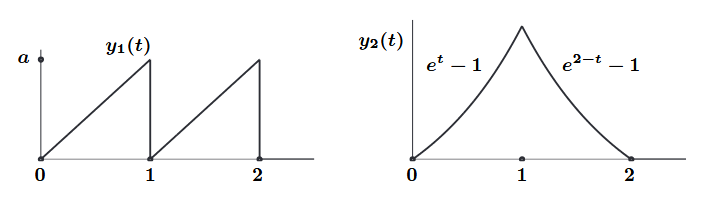
\includegraphics[width=1.0\textwidth]{../chap1/sec1.4/ex35.png}
\end{center}
The equation for \(y_{1} \!\left( t \right) \) is
\[
	y_{1} \!\left( t \right) = a R \!\left( t \right) \!\left( 1 - H \!\left( t - 1 \right)  \right) + a R \!\left( t - 1\right) \!\left( 1 - H \!\left( t - 2 \right)  \right) 
\]
For \(y_{2} \!\left( t \right) \), we have
\[
	y_{2} \!\left( t \right) = \!\left( e^{t} - 1 \right) \!\left( 1 - H \!\left( t - 1 \right)  \right) + \!\left( e^{2 - t} - 1 \right) H \!\left( t - 1 \right) 
\]
In the case of \(y_{1} \!\left( t \right) \), differentiate to find
\begin{align*}
	y_{1}' & = a \left[ H \!\left( t \right) \!\left( 1 - H \!\left( t - 1 \right)  \right)  - R \!\left( t \right) \delta \!\left( t - 1 \right) \right] \\
	       & \quad + a \left[ H \!\left( t - 1 \right) \!\left( 1 - H \!\left( t - 2 \right)  \right)  - R \!\left( t - 1 \right) \delta \!\left( t - 2 \right) \right] 
\end{align*}
This is a complicated-looking expression, so we will go by interval and study the behavior of the derivative as \(t\) increases.

First, over \(0 \le t < 1\), we have \(y_{1}' = a\). At precisely \(t = 1\), however, the first delta function kicks in, plunging \(y_{1}'\) down to \(-\infty\) at that very instant. Moving over \(1 < t < 2\), once again, \(y_{1}'\) is \(a\). At \(t = 2\), the second delta function sends \(y_{1}'\) to \(-\infty\) once more. In succinct terms, we may represent \(y_{1}'\) as
\[
	y_{1}' = a - \delta \!\left( t - 1 \right) - \delta \!\left( t - 2 \right) 
\]
where \(a\) (referring to \(a\) in the differential equation, not in the figure) is zero, and \(q \!\left( t \right) \) is the right-hand side.

Lastly, the derivative of \(y_{2}\) is
\begin{align*}
	y_{2}' & = -\!\left( e^{t} - 1 \right) \delta \!\left( t - 1 \right) + e^{t} \!\left( 1 - H \!\left( t - 1 \right)  \right) \\
	       & \quad \!\left( e^{2-t} - 1 \right) \delta \!\left( t - 1 \right) - e^{2 - t} H \!\left( t - 1 \right) 
\end{align*}
Once again, proceeding in intervals: first consider \(0 \le t < 1\). Then \(y_{2}' = e^{t}\), which is equivalent to \(y_{2} + 1\). Next we consider \(t > 1\). Here, \(y_{2}' = -e^{2 - t}\), or \(-y_{2} - 1\). At time \(t = 1\), we have a discontinuous jump in the derivative from \(e\) to \(-e\). Thus we have
\[
	y_{2}' = \begin{cases}
		y_{2} + 1 & 0 \le t < 1  \\
		- y_{2} - 1 & t > 1 \\
	\end{cases}
\]

\newpage
\subsection{\textsf{1.5 - Real and Complex Sinusoids}}
% QUESTION 1
\qs{1.5.1}{These steps lead again to the sinusoidal identity. This approach doesn't start with the usual formula \(\cos\left( \omega t - \phi \right) = \cos\left( \omega t \right) \cos\left( \phi \right) + \sin\left( \omega t \right) \sin\left( \phi \right)\) from trigonometry. The identity says:

\[
\textbf{If } \bm{A + iB = Re^{i \phi}} \textbf{ then } \bm{A \cos( \omega t)  + B \sin( \omega t ) = R \cos( \omega t - \phi ).}
\]
Here are the four steps to find that real part of \(Re^{i \!\left( \omega t - \phi \right) }\). Explain \(A - iB\) in Step 3.

\begin{align*}
	\bm{R \cos( \omega t - \phi )} & = \Real \left[ R e^{i \!\left( \omega t - \phi  \right) } \right] \\ 
	 & = \Real \left[ e^{i \omega t} \!\left( R e^{-i \phi } \right)  \right]  \\ 
	 & = \!\left( \textit{what is } R e^{-i \phi } \right) ? \\
	 & = \Real \left[ \!\left( \cos\left( \omega t \right) + i \sin\left( \omega t \right) \right) \!\left( A - i B \right)  \right] \\
	 & = \bm{A \cos (\omega t) + B \sin (\omega t) }
\end{align*}}

By Euler's formula, we have
\[
	Re^{-i \phi } = R \!\left( \cos \phi - i \sin \phi \right) 
\]
where \(A = R \cos \phi \) and \(B = R \sin \phi \).

% QUESTION 2
\qs{1.5.2}{To express \(\sin 5t + \cos 5t \) as \(R \cos\left( \omega t - \phi  \right)\), what are \(R\) and \(\phi \)?}

By the sinusoidal identity, \(A = R \cos \phi \) and \(B = R \sin \phi \). Thus \(A^{2} + B^{2} = 1 + 1 = 2\), implying \(R = \sqrt{2}\). For the phase lag, we have \(\tan \phi = 1\), implying \(\phi = \pi /4\). Thus
\[
	\sin 5t + \cos 5t = \sqrt{2} \cos\left( 5t - \pi /4 \right)
\]

% QUESTION 3
\qs{1.5.3}{To express \(6 \cos 2t + 8 \sin 2t\) as \(R \cos\left( 2t - \phi  \right)\), what are \(R\) and \(\tan \phi \) and \(\phi \)?}

By the sinusoidal identity, \(A = R \cos \phi \) and \(B = R \sin \phi \). Thus \(A^{2} + B^{2} = 6^{2} + 8^{2} = 36 + 64 = 100\), implying \(R = 10\). Moreover, \(\tan \phi = 4/3\), implying \(\phi = \arctan 4/3\). Thus
\[
	6 \cos 2t + 8 \sin 2t = 10 \cos\left( 2t - \arctan \frac{4}{3} \right)
\]

% QUESTION 4
\qs{1.5.4}{Integrate \(\cos \omega t\) to find \(\!\left( \sin \omega t \right) / \omega \) in this complex way.
\begin{enumerate}[label=(\roman*)]
	\item \(dy_{\text{real}} / dt = \cos \omega t\) is the real part of \(dy_{\text{complex}} / dt = e^{i \omega t}\).
	\item Take the real part of the complex solution.
\end{enumerate}}

(i) Integrate with respect to \(t\) to find:
\begin{alignat*}{3}
	&\implies && y_{\text{complex}} \!\left( t \right)  && = \int^{t}_{0} e^{i \omega s} \, ds   \\
	& && && = \frac{e^{i \omega t} - 1}{i \omega } \\ 
\end{alignat*}
Now, rewrite \(1/i \omega \) as \(\frac{1}{\omega } e^{-i \pi /2}\). Then we have
\[
	= \frac{1}{\omega } \!\left( e^{i \!\left( \omega t - \pi / 2 \right) } - e^{-i \pi / 2} \right) 
\]
(ii) which has real component
\[
	y_{\text{real}} \!\left( t \right) = \frac{1}{\omega } \cos\left( \omega t - \pi / 2 \right) = \frac{1}{\omega } \sin \omega t 
\]
Finally, we can see that the real component of \(dy_{\text{complex}} / dt\) is
\[
	dy_{\text{real}} / dt = \cos \omega t
\]
Enabling us to conclude that \(\cos \omega t\) integrates to \(\!\left( \sin \omega t \right) / \omega \).

\vspace{12pt}

% QUESTION 5
\qs{1.5.5}{The sinusoidal identity for \(A = 0\) and \(B = -1\) says that \(- \sin \omega t = R \cos\left( \omega t - \phi  \right)\). Find \(R\) and \(\phi\).}

By the sinusoidal identity, we have \(R^{2} = A^{2} + B^{2} = 1\), implying \(R = 1\). It turns out that the value of \(\phi \) lies at a discontinuity point of \(\tan\), namely at \(\phi = - \pi /2\). We derive the classic identity
\[
	- \sin \omega t = \cos\left( \omega t + \frac{\pi }{2}\right)
\]

% QUESTION 6
\qs{1.5.6}{Why is the sinusoidal identity useless for the source \(q \!\left( t \right) = \cos t + \sin 2t\)?}

The frequency differs between the terms.

\vspace{12pt}

% QUESTION 7
\qs{1.5.7}{Write \(2 + 3i\) as \(re^{i \phi }\), so that \(\frac{1}{2 + 3i} = \frac{1}{r} e^{-i \phi }\). Then write \(y = e^{i \omega t} / \!\left( 2 + 3i \right) \) in polar form. Then find the real and imaginary parts of \(y\). And also find those real and imaginary parts directly from \(\!\left( 2 - 3i \right) e^{i \omega t} / \!\left( 2 - 3i \right) \!\left( 2 + 3i \right) \).}

With \(2 + 3i\), we have \(R^{2} = 2^{2} + 3^{2} = 4 + 9 = 13\), implying \(R = \sqrt{13}\). Additionally, we have \(\tan \phi = 3/2\), implying \(\phi = \arctan 3/2 \). In polar form, we have
\[
	2 + 3i = \sqrt{13} e^{i \arctan 3/2}
\]
The inverse is
\[
	\frac{1}{2 + 3i} = \frac{1}{\sqrt{13}} e^{-i \arctan 3/2}
\]
And in polar form, \(y = e^{i \omega t}/ \!\left( 2 + 3i \right) \) is given by
\[
	y = \frac{e^{i \omega t}}{2 + 3i} = \frac{1}{\sqrt{13}} e^{i \!\left( \omega t - \arctan 3/2 \right) }
\]
which has real and imaginary parts
\[
	\Real \left[ y \right] = \frac{1}{\sqrt{13}} \cos\left( \omega t - \arctan 3/2 \right) \qquad \Imag \left[ y \right] = \frac{1}{\sqrt{13}} \sin\left( \omega t - \arctan 3/2 \right)
\]
Calculating by way of the complex conjugate, we find
\begin{alignat*}{3}
	&\implies && \frac{e^{i \omega t}}{2 + 3i} && = \frac{\!\left( 2 - 3i \right) e^{i \omega t}}{\!\left( 2 - 3i \right) \!\left( 2 + 3i \right) } \\
	& && && = \frac{\!\left( 2 - 3i \right) \!\left( \cos \omega t + i \sin \omega t \right) }{13}  \\
	& && && = \frac{2 \cos \omega t + 3 \sin \omega t + i \!\left( 2 \sin \omega t - 3 \cos \omega t \right) }{13} \\
	&\implies && \Real \left[ y \right] && = \frac{1}{13} \!\left( 2 \cos \omega t + 3 \sin \omega t\right) \\
	&\implies && \Imag \left[ y \right] && = \frac{1}{13} \!\left( 2 \sin \omega t - 3 \cos \omega t \right) 
\end{alignat*}

% QUESTION 8
\qs{1.5.8}{Write these functions \(A \cos \omega t + B \sin \omega t\) in the form \(R \cos\left( \omega t - \phi  \right)\): Right triangle with sides \(A\), \(B\), \(R\) and angle \(\phi \).
\begin{enumerate}[label=(\arabic*)]
	\item \(\cos 3t - \sin 3t\)
	\item \( \sqrt{3} \cos \pi t - \sin \pi t \)
	\item \( 3 \cos\left( t - \phi  \right) + 4 \sin\left( t - \phi  \right) \)
\end{enumerate}}

(1) Here, \(A = 1\) and \(B = -1\). Then \(R^{2} = A^{2} + B^{2} = 1^{2} + \!\left( -1 \right)^{2} = 2\), implying \(R = \sqrt{2}\). Furthermore, \(\tan \phi = -1\) implies \(\phi = -\pi / 4\). Thus
\[
	\cos 3t - \sin 3t = \sqrt{2} \cos\left( 3t + \frac{\pi }{4} \right)
\]
(2) Here, \(A = \sqrt{3}\) and \(B = -1\). Then \(R^{2} = A^{2} + B^{2} = \!\left( \sqrt{3} \right)^{2} + \!\left( -1 \right)^{2} = 4\), implying \(R = 2\). Furthermore, \(\tan \phi = -1 / \sqrt{3}\) implies \(\phi = - \pi / 6\). Thus
\[
	\sqrt{3} \cos \pi t - \sin \pi t = 2 \cos\left( \pi t + \pi / 6 \right)
\]
(3) Here, \(A = 3\) and \(B = 4\). Then \(R^{2} = A^{2} + B^{2} = 3^{2} + 4^{2} = 25\), implying \(R = 5\). Furthermore, \(\tan \alpha  = 4/3\) implies \(\alpha  = \arctan 4/3\). Thus
\[
	3 \cos\left( t - \phi  \right) + 4 \sin\left( t - \phi  \right) = 5 \cos\left( t - \phi - \arctan 4/3 \right)
\]

% QUESTION 9
\qs{1.5.9}{Solve \(dy/dt = 2y + 3 \cos t + 4 \sin t\) after recognizing \(a\) and \(\omega \). Null solutions \(C e^{2t}\).}

Let \(y = M \cos t + N \sin t\). Then \(dy / dt = - M \sin t + N \cos t\). Subtracting \(2y\) from both sides yields
\begin{alignat*}{3}
	&\implies && dy / dt - 2y && = 3 \cos t + 4 \sin t \\
	&\implies && \!\left( N - 2M \right)  \cos t - \!\left( 2N + M \right)  \sin t && = 3 \cos t + 4 \sin t 
\end{alignat*}
Here, we may conclude that \(N - 2M = 3\) and \(- \!\left( 2N + M \right)= 4\). Solving for the unknowns corresponds to the matrix equation
\[
	\begin{bmatrix}
		1 & -2 \\
		-2 & -1 \\
	\end{bmatrix}
\begin{bmatrix}
N	 \\
M	 \\
\end{bmatrix}
=
\begin{bmatrix}
	3 \\
	4 \\
\end{bmatrix}
\]
which is a matter of solving
\[
	\begin{bmatrix}
		N \\
		M \\
	\end{bmatrix}
=
\begin{bmatrix}
	1/5 & -2/5 \\
	-2/5 & -1/5 \\
\end{bmatrix}
\begin{bmatrix}
	3 \\
	4 \\
\end{bmatrix}
=
\begin{bmatrix}
	-1 \\
	-2 \\
\end{bmatrix}
\]
Thus we have
\[
	y_{p} \!\left( t \right) = -2 \cos t - \sin t
\]
and combining the null solutions \(Ce^{2t}\), we have complete solution
\[
	y \!\left( t \right) = Ce^{2t} - 2 \cos t - \sin t
\]
% QUESTION 10	
\qs{1.5.10}{Find a particular solution to \(dy/dt = -y - \cos 2t\).}

Let \(y = M \cos 2t + N \sin 2t\). Then \(dy/dt = - 2M \sin 2t + 2N \cos 2t\). We derive
\begin{alignat*}{3}
	&\implies && dy / dt + y && = - \cos 2t \\
	&\implies && \!\left( 2N + M \right) \cos 2t + \!\left( N - 2M \right) \sin 2t && = -\cos 2t \\ 
\end{alignat*}
Allowing us to conclude \(2N + M = -1\) and \(N - 2M = 0\), or \(N = 2M\). Substitution gives us \(N = -2/5\), \(M = -1/5\), and particular solution
\[
	y_{p} \!\left( t \right) = - \frac{1}{5} \cos 2t - \frac{2}{5} \sin 2t
\]

% QUESTION 11
\qs{1.5.11}{What equation \(y' - ay = A \cos \omega t + B \sin \omega t\) is solved by \(y = 3 \cos 2t + 4 \sin 2t\)?}

We can derive \(y' = -6 \sin 2t + 8 \cos 2t\), giving us on the left-hand side:
\[
	\!\left( 8 \cos 2t - 6 \sin 2t \right) - a \!\left( 3 \cos 2t + 4 \sin 2t \right) = \!\left( 8 - 3a \right) \cos 2t - \!\left( 6 + 4a \right) \sin 2t 
\]

Thus \(A = 8 - 3a\) and \(B = - \!\left( 6 + 4a \right) \), and the desired equation is:
\[
	y' - ay = \!\left( 8 - 3a \right) \cos \omega t - \!\left( 6 + 4a \right) \sin \omega t
\]

% QUESTION 12
\qs{1.5.12}{The particular solution to \(y' = y + \cos t\) in Section 1.4 is \(y_{p} = e^{t} \int e^{-s} \cos s \, ds\). Look this up or integrate by parts, from \(s = 0\) to \(t\). Compare this \(y_{p}\) to formula (3).}

Integrating by parts, we have
\[
	y_{p} = e^{t} \int^{t}_{0} e^{-s} \cos s \, ds 
\]
where we let \(u = e^{-s}\) and \(dv = \cos s \, ds\). Then \(du = -e^{-s} \, ds\) and \(v = \sin s\), and we have
\[
	y_{p} = e^{t} \left[ e^{-t} \sin t + \int^{t}_{0} e^{-s} \sin s \, ds   \right] 
\]
In the second term, let \(u^{*} = e^{-s}\) and \(dv^{*} = \sin s \, ds \). Then \(du^{*} = -e^{-s} \, ds \) and \(v^{*} = -\cos s\). We further evaluate as
\[
	y_{p} = e^{t} \left[ e^{-t} \sin t - e^{-t} \cos t + 1 - \int^{t}_{0} e^{-s} \cos s \, ds   \right] 
\]
Now, using our original \(y_{p}\), we can add \(e^{t} \int e^{-s} \cos s \, ds \) to both sides to derive
\begin{align*} 
	2e^{t} \int^{t}_{0} e^{-s} \cos s \, ds & = e^{t} \left[ e^{-t} \sin t - e^{-t} \cos t + 1 \right] \\
						& = \sin t - \cos t + e^{t}
\end{align*}
and concluding with
\[
	y_{p} = \frac{1}{2} \!\left( \sin t - \cos t + e^{t} \right) 
\]
Comparing to formula (3) of section 1.5, we have \(a = \omega = 1\), \(A = 1\), \(B = 0\), and as such,
\[
	M = -\frac{\!\left( 1 \right) \!\left( 1 \right) }{1^{2} + 1^{2}} = -\frac{1}{2} \qquad N = \frac{\!\left( 1 \right) \!\left( 1 \right) }{1^{2} + 1^{2}} = \frac{1}{2}
\]

% QUESTION 13
\qs{1.5.13}{Find a solution \(y = M \cos \omega t + N \sin \omega t\) to \(y' - 4y = \cos 3t + \sin 3t\).}

Derive \(y' = -M \omega \sin \omega t + N \omega \cos \omega t\). Then we have
\begin{align*}
	\!\left( - M \omega \sin \omega t + N \omega \cos \omega t \right) & - 4 \!\left( M \cos \omega t + N \sin \omega t \right) = \\
	& \quad \!\left( -4M + N \omega  \right) \cos \omega t + \!\left( -M \omega - 4N \right) \sin \omega t 
\end{align*}

Here, we have \(\omega = 3\). Then we have the system of linear equations
\[
	-4M + 3N = 1 \qquad -3M - 4N = 1
\]
The corresponding matrix equation is
\[
	\begin{bmatrix}
		-4 & 3 \\
		-3 & -4 \\
	\end{bmatrix}
\begin{bmatrix}
	M \\
	N \\
\end{bmatrix}
=
\begin{bmatrix}
	1 \\
	1 \\
\end{bmatrix}
\]
which has solution
\[
	\begin{bmatrix}
		M \\
		N \\
	\end{bmatrix}
=
\begin{bmatrix}
	-4/25 & -3/25 \\
	3/25 & -4/25 \\
\end{bmatrix}
\begin{bmatrix}
	1 \\
	1 \\
\end{bmatrix}
=
\begin{bmatrix}
	-7/25 \\
	-1/25 \\
\end{bmatrix}
\]
Thus we have particular solution
\[
	y = -\frac{7}{25} \cos 3t -\frac{1}{25} \sin 3t 
\]

% QUESTION 14
\qs{1.5.14}{Find the solution to \(y' - ay = A \cos \omega t + B \sin \omega t\) \textbf{starting from} \(\bm{y \!\left( 0 \right) = 0}\).}

Let \(y \!\left( t \right) = M \cos \omega t + N \sin \omega t + Ce^{at}\). Then we have \(y \!\left( 0 \right) = M + C\), which vanishes by premise. Ergo, \(C = - M\), and we end up with
\[
	y \!\left( t \right) = M \cos \omega t + N \sin \omega t - M e^{at}
\]
where \(M, N\) are given in terms of
\[
	M = -\frac{aA + \omega B}{\omega^{2} + a^{2}} \qquad N = \frac{\omega A - aB}{\omega^{2} + a^{2}}
\]

% QUESTION 15
\qs{1.5.15}{If \(a = 0\) show that \(M\) and \(N\) in equation (3) still solve \(y' = A \cos \omega t + B \sin \omega t\).}

Let \(y = M \cos \omega t + N \sin \omega t\). Then
\[
	y' = -M \omega \sin \omega t + N \omega \cos \omega t
\]
Ascertaining that
\begin{align*}
	A = N \omega  & \implies N = \frac{A}{\omega } \\
	B = -M \omega  & \implies M = -\frac{B}{\omega } \\ 
\end{align*}
which is indeed formula (3) when \(a = 0\).

% QUESTION 16
\qs{1.5.16}{Write down complex solutions \(y_{p} = Ye^{i \omega t}\) to these three equations:
\begin{enumerate}[label=(\alph*)]
	\item \(y' - 3y = 5e^{2it}\)
	\item \(y' = Re^{i \!\left( \omega t - \phi  \right) }\)
	\item \(y' = 2y - e^{it}\)
\end{enumerate}}

(a) We have \(\omega = 2\). Let \(y = Ye^{2it}\). Then \(y' = 2Yie^{2it}\), and we have
\begin{alignat*}{3}
	&\implies && 2Yie^{2it} - 3Ye^{2it} && = 5e^{2it} \\
	&\implies && 2Yi - 3Y && = 5 \\ 
	&\implies && Y && = \frac{5}{-3 + 2i}
\end{alignat*}
Then
\[
	y_{p} = \!\left( \frac{5}{-3 + 2i} \right) e^{2it}
\]
(b) Let \(y = Ye^{i \omega t}\). Then \(y' = i \omega Ye^{i \omega t}\), so we have
\begin{alignat*}{3}
	&\implies && i \omega Ye^{i \omega t} && = Re^{i \!\left( \omega t - \phi  \right) } \\
	&\implies && Y && = \frac{Re^{-i \phi }}{i \omega }
\end{alignat*}
Ergo, we have
\[
	y = \frac{Re^{i \!\left( \omega t - \phi  \right) }}{i \omega }
\]

(c) Let \(y = Ye^{it }\). We have \(\omega = -1\). Then \(y' = iYe^{it }\), and
\begin{alignat*}{3}
	&\implies && iYe^{it } - 2Ye^{it } && = -e^{it } \\
	&\implies && iY - 2Y && = -1 \\ 
	&\implies && Y && = \frac{1}{2 - i}
\end{alignat*}
Thus we have
\[
	y = \!\left( \frac{1}{2 - i} \right) e^{it}
\]

% QUESTION 17
\qs{1.5.17}{Find complex solutions \(z_{p} = Ze^{i \omega t}\) to these complex equations:
\begin{enumerate}[label=(\alph*)]
	\item \(z' + 4z = e^{8it}\)
	\item \(z' + 4iz = e^{8it}\)
	\item \(z' + 4iz = e^{8t}\)
\end{enumerate}}

(a) We have \(\omega = 8\). Let \(z = Ze^{8it}\). Then we have
\begin{alignat*}{3}
	&\implies && 8iZe^{8it } + 4Ze^{8it } && = e^{8it } \\
	&\implies && 8iZ + 4Z && = 1 \\
	&\implies && Z && = \frac{1}{4 + 8i} \\ 
\end{alignat*}
Then
\[
	z_{p} = \!\left( \frac{1}{4 + 8i} \right) e^{8it }
\]
(b) We have \(\omega = 8\). Let \(z = Ze^{8it }\). Then we have
\begin{alignat*}{3}
	&\implies && 8iZe^{8it } + 4iZe^{8it} && = e^{8it } \\
	&\implies && 8iZ + 4iZ && = 1 \\ 
	&\implies && Z && = \frac{1}{12i}
\end{alignat*}
Ergo, we have
\[
	z_{p} = \frac{e^{8it }}{12i}
\]
(c) Let \(z = Ze^{8t}\). Then we have
\begin{alignat*}{3}
	&\implies && 8Ze^{8t} + 4iZe^{8t} && = e^{8t} \\
	&\implies && 8Z + 4iZ && = 1 \\ 
	&\implies && Z && = \frac{1}{8 + 4i}
\end{alignat*}
Ergo, we have
\[
	z_{p} = \frac{1}{8 + 4i} e^{8it}
\]

% QUESTION 18
\qs{1.5.18}{Start with the real equation \(y' - ay = R \cos\left( \omega t - \phi  \right)\). Change to the complex equation \(z' - az = Re^{i \!\left( \omega t - \phi  \right) }\). Solve for \(z \!\left( t \right) \). Then take its real part \(y_{p} = \Real z\).}

Let \(z = Ze^{i \omega t}\). Then we have
\begin{alignat*}{3}
	&\implies && i \omega Ze^{i \omega t} - aZe^{i \omega t} && = Re^{i \!\left( \omega t - \phi  \right) } \\
	&\implies && i \omega Z - aZ && = Re^{-i \phi } \\ 
	&\implies && Z && = \frac{Re^{-i \phi }}{i \omega - a}
\end{alignat*}
And we have solution
\begin{align*}
	z \!\left( t \right) & = \frac{Re^{i \!\left( \omega t - \phi  \right) }}{i \omega - a} \\
			     & = \frac{Re^{i \!\left( \omega t - \phi  \right) }}{i \omega - a} \frac{i \omega + a}{i \omega + a} \\
			     & = R \frac{\!\left(\cos\left( \omega t - \phi  \right) + i \sin\left( \omega t - \phi  \right)\right) \!\left( i \omega + a \right) }{\!\left( i \omega - a \right) \!\left( i \omega + a \right) } \\
			     & = -R \frac{a \cos\left( \omega t - \phi  \right) - \omega \sin\left( \omega t - \phi  \right) + i \!\left( \omega \cos\left( \omega t - \phi  \right) + a \sin\left( \omega t - \phi  \right) \right) }{a^{2} + \omega^{2} }
\end{align*}
which has real part
\[
	y_{p} = \Real z \!\left( t \right) = -\frac{R}{a^{2} + \omega^{2}} \!\left( a \cos\left( \omega t - \phi  \right) - \omega \sin\left( \omega t - \phi  \right) \right) 
\]

% QUESTION 19
\qs{1.5.19}{What is the initial value \(y_{p} \!\left( 0 \right) \) of the particular solution \(y_{p}\) from Problem 18? If the desired initial value is \(y \!\left( 0 \right) \), how much of the null solution \(y_{n} = Ce^{at}\) would you add to \(y_{p}\)?}

The initial value of the particular solution is
\begin{align*}
	y_{p} \!\left( 0 \right) & = -\frac{R}{a^{2} + \omega^{2}} \!\left( a \cos\left( - \phi  \right) - \omega \sin\left( -\phi  \right) \right) \\
				 & = -\frac{R}{a^{2} + \omega^{2}} \!\left( a \cos\left( \phi  \right) + \omega \sin\left( \phi  \right) \right) 
\end{align*}

For the complete solution to have initial condition \(y \!\left( 0 \right) = 0\), we must have null solution
\[
	y_{n} = \frac{R}{a^{2} + \omega^{2}} \!\left( a \cos\left( \phi  \right) + \omega \sin\left( \phi  \right) \right) e^{at}
\]

% QUESTION 20
\qs{1.5.20}{Find the real solution to \(y' - 2y = \cos \omega t\) starting from \(y \!\left( 0 \right) = 0\), in three steps: Solve the complex equation \(z' - 2z = e^{i \omega t}\), take \(y_{p} = \Real z\), and add the null solution \(y_{n} = Ce^{2t}\) with the right \(C\).}

First, in solving the complex equation, let \(z = Ze^{i \omega t}\). Then we have
\begin{alignat*}{3}
	&\implies && i \omega Ze^{i \omega t} - 2Ze^{i \omega t} && = e^{i \omega t} \\
	&\implies && i \omega Z - 2Z && = 1 \\ 
	& \implies && Z && = \frac{1}{i \omega - 2}
\end{alignat*}
Giving us solution
\[
	z \!\left( t \right) = \frac{1}{i \omega - 2} e^{i \omega t}
\]
which we rewrite as
\begin{align*}
	z \!\left( t \right)  & = \!\left( \cos\left( \omega t \right) + i \sin\left( \omega t \right) \right) \!\left( \frac{1}{i \omega - 2} \right) \!\left( \frac{i \omega + 2}{i \omega + 2} \right)  \\
	 & = - \!\left( \cos\left( \omega t \right) + i \sin\left( \omega t \right) \right) \!\left( \frac{i \omega + 2}{4 + \omega^{2}} \right)  \\
	 & = -\frac{1}{4 + \omega^{2}} \!\left( 2 \cos\left( \omega t \right) - \omega \sin\left( \omega t \right) + i \!\left( \omega \cos\left( \omega t \right) + 2 \sin\left( \omega t \right) \right)  \right) 
\end{align*}

The real component is given by
\[
	y_{p} = \Real z \!\left( t \right) = -\frac{1}{4 + \omega^{2}} \!\left( 2 \cos\left( \omega t \right) - \omega \sin\left( \omega t \right) \right) 
\]
which has initial condition
\[
	y_{p} = - \frac{2}{4 + \omega^{2}}
\]
Lastly, to satisfy the initial solution \(y \!\left( 0 \right) = 0\), we have null solution
\[
	y_{n} = \frac{2}{4 + \omega^{2}} e^{2t}
\]
Thus the complete solution is
\[
	y \!\left( t \right) = \frac{2}{4 + \omega^{2}}e^{2t} - \frac{1}{4 + \omega^{2}} \!\left( 2 \cos\left( \omega t \right) - \omega \sin\left( \omega t \right) \right) 
\]

% QUESTION 21
\qs{1.5.21}{Find \(r\) and \(\alpha \) to write each \(i \omega - a\) as \(re^{i \alpha }\). Then write \(1 / re^{i \alpha }\) as \(Ge^{-i \alpha }\).
\begin{enumerate}[label=(\alph*)]
	\item \(\sqrt{3}i + 1\)
	\item \(\sqrt{3}i - 1\)
	\item \(i - \sqrt{3}\)
\end{enumerate}}

(a) We have \(r^{2} = 1^{2} + \!\left( \sqrt{3} \right)^{2} = 4 \), implying \(r = 2\). Moreover, \(\tan \alpha = \sqrt{3}\), implying \(\alpha = \pi / 3\). The polar form is
\[
	2e^{i \pi / 3}
\]
and its inverse is
\[
	\frac{1}{2e^{i \pi / 3}} = \frac{1}{2} e^{-i \pi /3}
\]
(b) We have \(r = 2\) once more. Additionally, \(\tan \alpha = -\sqrt{3}\), implying \(\alpha = 2 \pi / 3\). The polar form is
\[
	2e^{i 2 \pi / 3}
\]
and its inverse is
\[
        \frac{1}{2 e^{i 2\pi /3}} = \frac{1}{2} e^{- i 2\pi / 3}
\]
(c) We have \(r = 2\) once more. Additionally, \(\tan \alpha = -1 / \sqrt{3}\), implying \(\alpha = 5 \pi / 6\). The polar form is
\[
	2e^{i 5 \pi / 6} 
\]
and its inverse is
\[
	\frac{1}{2e^{i 5 \pi / 6}} = \frac{1}{2} e^{-i 5 \pi / 6}
\]

% QUESTION 22
\qs{1.5.22}{Use \(G\) and \(\alpha \) from Problem 21 to solve (a)-(b)-(c). Then take the real part of each equation and the real part of each solution.
\begin{enumerate}[label=(\alph*)]
	\item \(y' + y = e^{i \sqrt{3}t}\)
	\item \(y' - y = e^{i \sqrt{3}t}\)
	\item \(y' - \sqrt{3}y = e^{it }\)
\end{enumerate}}

(a) We have \(\omega = \sqrt{3}\) and \(a = -1\), corresponding to complex solution
\[
	y_{c} = \frac{1}{2} e^{i \!\left( \sqrt{3} t - \pi / 3 \right) }
\]
which has real component
\[
	y_{p} = \frac{1}{2} \cos\left( \sqrt{3}t - \frac{\pi }{3}\right)
\]
(b) We have \(\omega = \sqrt{3}\) and \(a = 1\), corresponding to complex solution
\[
	y_{c} = \frac{1}{2} e^{i \!\left( \sqrt{3}t - 2 \pi / 3 \right) }
\]
which has real component
\[
	y_{p} = \frac{1}{2} \cos\left( \sqrt{3}t - \frac{2 \pi }{3} \right)
\]
(c) We have \(\omega = 1\) and \(a = \sqrt{3}\), corresponding to complex solution
\[
	y_{c} = \frac{1}{2} e^{i \!\left( t - 5 \pi / 6 \right) }
\]
which has real component
\[
	y_{p} = \frac{1}{2} \cos\left( t - \frac{5 \pi }{6} \right)
\]

% QUESTION 23
\qs{1.5.23}{Solve \(y' - y = \cos \omega t + \sin \omega t\) in three steps: real to complex, solve complex, take real part. This is an important example.
\begin{enumerate}[label=(\arabic*)]
	\item Find \(R\) and \(\phi \) in the sinusoidal identity to write \(\cos \omega t + \sin \omega t\) as the real part of \(Re^{i \!\left( \omega t - \phi  \right) }\).
	\item Solve \(y' - y = e^{i \omega t}\) by \(y = Ge^{-i \alpha } e^{i \omega t}\). Multiply by \(Re^{-i \phi }\) to solve \(z' - z = R e^{i \!\left( \omega t - \phi  \right) }\).
	\item Take the real part \(y \!\left( t \right) = \Real z \!\left( t \right) \). Check that \(y' - y = \cos \omega t + \sin \omega t\).
\end{enumerate}}

(1) By the sinusoidal identity, \(R^{2} = A^{2} + B^{2} = 1^{2} + 1^{2} = 2\), implying \(R = \sqrt{2}\). Additionally, \(\tan \phi = B/A = 1\), implying \(\phi = \pi / 4\). Then \(\cos \omega t + \sin \omega t\) is equal to
\[
	\Real \sqrt{2} e^{i \!\left( \omega t - \pi / 4 \right) } = \sqrt{2} \cos\left( \omega t - \frac{\pi }{4} \right)
\]
(2) Take \(y = Ge^{-i \alpha } e^{i \omega t}\). We have \(\omega \) and \(a = 1\). Then for \(G\) and \(\alpha \), we find
\[
	G = \frac{1}{\sqrt{\omega^{2} + 1}} \qquad \alpha = \arctan \!\left( -\omega  \right)  
\]
Then we have
\[
	y \!\left( t \right)  = \frac{1}{\sqrt{\omega^{2} + 1}} e^{i \!\left(\omega t - \alpha  \right)}
\]
Multiplying by \(Re^{-i \phi } = \sqrt{2} e^{- i\pi / 4 }\) yields the complex solution
\[
	z \!\left( t \right)  = \sqrt{\frac{2}{\omega^{2} + 1}}e^{i \!\left( \omega t - \alpha - \pi / 4 \right) } 
\]
(3) which in turn has real component
\[
	y \!\left( t \right) = \Real z \!\left( t \right) = \sqrt{\frac{2}{\omega^{2} + 1}} \cos\left( \omega t - \alpha - \frac{\pi }{4} \right)
\]
Observe that if \(\omega = 1\), then we have \(\alpha = \arctan \!\left( -1 \right) \), which for complex number \(\displaystyle{\frac{1}{i \omega - 1}}\) corresponds to \(\alpha = 3 \pi / 4\). Then we have real solution
\[
	y \!\left( t \right) = \cos\left( t - \pi  \right) = - \cos\left( t \right)
\]

% QUESTION 24
\qs{1.5.24}{Solve \(y' - \sqrt{3}y = \cos t + \sin t\) by the same three steps with \(a = \sqrt{3}\) and \(\omega = 1\).}

(1) We have \(A = B = 1\), so \(R = \sqrt{2}\), and \(\tan \phi = 1\) implies \(\phi = \pi / 4\). Thus by the sinusoidal identity, we have
\[
	\Real \sqrt{2} e^{i \!\left( t - \pi / 4 \right) } = \sqrt{2} \cos\left( t - \frac{\pi }{4} \right)
\]

(2) With \(a = \sqrt{3}\) and \(\omega = 1\), we have gain and phase angle
\[
	G = \frac{1}{2} \qquad \alpha = \frac{5 \pi }{6}
\]
Giving us the complex solution
\[
	z \!\left( t \right) = \frac{1}{\sqrt{2}}e^{i \!\left( t - 13 \pi /12 \right) }
\]
(3) The real component to \(z \!\left( t \right) \) is
\[
	\Real z \!\left( t \right) = \frac{1}{\sqrt{2}} \cos\left( t - \frac{13 \pi }{12} \right)
\]

% QUESTION 25
\qs{1.5.25}{\textbf{(Challenge)} Solve \(y' - ay = A \cos \omega t + B \sin \omega t\) in two ways. First, find \(R\) and \(\phi \) on the right and \(G\) and \(\alpha \) on the left. Show that the final real solution \(RG \cos\left( \omega t - \phi - \alpha  \right)\) agrees with \(M \cos \omega t + N \sin \omega t\) in equation (2).}

We have the following quantities:
\begin{align*}
	R & = \sqrt{A^{2} + B^{2}} \\
	G & = \frac{1}{\sqrt{\omega^{2} + a^{2}}} \\ 
	\phi & = \arctan \!\left( \frac{B}{A} \right) \\
	\alpha & = \arctan \!\left( -\frac{\omega }{a} \right) + \pi 
\end{align*}
Observe the additional \(\pi \) term for \(\alpha \), which is necessary because for \(\omega\), \(a > 0\), the phase angle would be located in the second quadrant. In evaluating
\[
	RG \cos\left( \omega t - \phi - \alpha  \right)
\]
The quandary is to simplify the sum of the inverse tangent terms \(\phi \) and \(\alpha \), namely \(\phi + \alpha \). The following identity is of use to us:
\[
	\arctan a + \arctan b = \arctan \!\left( \frac{a + b}{1 - ab} \right) 
\]
We derive
\begin{align*}
	\phi + \alpha = \arctan \!\left( \frac{B}{A} \right) + \arctan \!\left( -\frac{\omega}{\alpha } \right) + \pi  & = \arctan \!\left( \frac{B/A - \omega / a}{1 + \omega B / aA} \right) + \pi  \\
	 & = \arctan \!\left( \frac{aB - \omega A}{aA + \omega B} \right) + \pi  \\ 
	 & = - \arctan \!\left( \frac{\omega A - aB}{aA + \omega B} \right) + \pi 
\end{align*}

Now, using the angle-difference trigonometric identity, we have
\[
	RG \cos\left( \omega t - \phi - \alpha  \right) = RG \left[  \cos\left( \omega t \right) \cos\left( \phi + \alpha  \right) + \sin \!\left( \omega t \right) \sin \!\left( \phi + \alpha  \right) \right]
\]
Next, using the following identities:
\[
	\cos\left( \arctan x \right) = \frac{1}{\sqrt{1 + x^{2}}} \qquad \sin\left( \arctan x \right) = \frac{x}{\sqrt{1 + x^{2}}}
\]
we may calculate:
\begin{align*}
	\cos\left( \phi + \alpha  \right) & = \cos\left( - \arctan \!\left( \frac{\omega A - aB}{aA + \omega B} \right) + \pi  \right) \\
	 & = -\sqrt{\frac{\!\left( aA + \omega B \right)^{2}}{\!\left( \omega A - aB \right)^{2} + \!\left( aA + \omega B \right)^{2}}} \\
	 & = -\frac{aA + \omega B}{\sqrt{\!\left( A^{2} + B^{2} \right) \!\left( \omega^{2} + a^{2} \right) }} \\
	\implies RG \cos\left( \phi + \alpha  \right) & = \boxed{-\frac{aA + \omega B}{\omega^{2} + a^{2}}} \\
	\sin\left( \phi + \alpha  \right) & = \sin\left( -\arctan \!\left( \frac{\omega A - aB}{aA + \omega B} \right) + \pi  \right) \\
		& = \frac{\omega A - aB}{\sqrt{\!\left( aB - \omega A \right)^{2} + \!\left( aA + \omega B \right)^{2}}} \\
		& = \frac{\omega A - aB}{\sqrt{\!\left( A^{2} + B^{2} \right) \!\left( \omega^{2} + a^{2} \right) }} \\
	\implies RG \sin\left( \phi + \alpha  \right) & = \boxed{\frac{\omega A - aB}{\omega^{2} + a^{2}}}
\end{align*}
where we employ the fact that
\begin{align*}
	\!\left( \omega A - aB \right)^{2} + \!\left( aA + \omega B \right)^{2} & = \omega^{2}A^{2} - 2a \omega AB + a^{2}B^{2} \\
	 & \qquad + a^{2} A^{2} + 2a \omega AB + \omega^{2} B^{2} \\ 
	 & = A^{2} \!\left( \omega^{2} + a^{2} \right) + B^{2} \!\left( \omega^{2} + a^{2} \right) \\
	 & = \!\left( A^{2} + B^{2} \right) \!\left( \omega^{2} + a^{2} \right) 
\end{align*}
Finally, we may conclude that \(RG \cos\left( \phi + \alpha  \right) = M\) and \(RG \sin\left( \phi + \alpha  \right) = N\).

\vspace{12pt}

% QUESTION 26
\qs{1.5.26}{We don't have resonance for \(y' - ay = Re^{i \omega t}\) when \(a\) and \(\omega \neq 0\) are real. \textit{Why not?} (Resonance appears when \(y_{n} = Ce^{at}\) and \(y_{p} = Ye^{ct}\) share the exponent \(a = c\).)}

Under the premises, we have \(a \in \mathbb{R}\) and \(i \omega \not\in\mathbb{R}\). Therefore, they can never be equal, and thus we can never have resonance.

\vspace{12pt}

% QUESTION 27
\qs{1.5.27}{If you took the imaginary part \(y = \Imag z\) of the complex solution to \(z' - az = Re^{i \!\left( \omega t - \phi  \right) }\), what equation would \(y \!\left( t \right) \) solve? Answer first with \(\phi = 0\).}

From exercise 18, we have
\[
	\Imag z \!\left( t \right) = -\frac{R}{a^{2} + \omega^{2}} \!\left( \omega \cos\left( \omega t - \phi  \right) + a \sin\left( \omega t - \phi  \right) \right) 
\]
This solution would solve
\[
	y' - ay = R \sin\left( \omega t - \phi  \right)
\]
In the case of \(\phi = 0\), we have the differential equation
\[
	y' - ay = R \sin\left( \omega t \right)
\]

% QUESTION 28
\qs{1.5.28}{Solve \(L dI / dt + RI \!\left( t \right) = V \cos \omega t\) for the current \(I \!\left( t \right) = I_{n} + I_{p}\) in the \(RL\) loop.}

\(\bm{I_{n} \!\left( t \right) }\): First we derive the null solution. We have equation
\[
	LI_{n}' \!\left( t \right) + RI_{n} \!\left( t \right)  = 0
\]
which we rewrite as
\[
	I_{n}'\!\left( t \right)  + \frac{R}{L}I_{n} \!\left( t \right)  = 0
\]
Using the integrating factor \(e^{\!\left( R/L \right) t}\), we derive the null solution as
\begin{alignat*}{3}
	&\implies && \!\left( e^{\!\left( R/L \right) t} I_{n} \!\left( t \right)  \right)' && = 0 \\
	&\implies && e^{\!\left( R/L \right) t} I_{n} \!\left( t \right) && = I \!\left( 0 \right)   \\
	&\implies && I_{n} \!\left( t \right) && = I \!\left( 0 \right) e^{-\!\left( R/L \right) t}
\end{alignat*}

\(\bm{I_{p} \!\left( t \right) }\): For our particular solution, we have equation
\[
	I_{p}' \!\left( t \right) + \frac{R}{L} I_{p} \!\left( t \right) = \frac{V}{L} \cos\left( \omega t \right)
\]
which we convert into a complex equation
\[
	a' \!\left( t \right) + \frac{R}{L} a \!\left( t \right) = \frac{V}{L} e^{i \omega t}
\]
Now, let \(a \!\left( t \right) = A e^{i \omega t}\). To find \(A\), derive
\begin{alignat*}{3}
	&\implies && i \omega A e^{i \omega t} + \frac{R}{L} A e^{i \omega t} && = \frac{V}{L} e^{i \omega t} \\
	&\implies && i \omega A + \frac{R}{L}A && = \frac{V}{L} \\ 
	&\implies && A && = \frac{V}{L \!\left( i \omega + R/L \right) } \\
	& && && = \frac{V}{i \omega L + R}
\end{alignat*}

This corresponds to gain and phase angle
\[
	G = \frac{1}{\sqrt{R^{2} + \omega^{2} L^{2}}} \qquad \alpha = \arctan \!\left( \frac{\omega L}{R} \right) 
\]
giving us complex solution
\[
	a \!\left( t \right) = \frac{V}{\sqrt{R^{2} + \omega^{2}L^{2}}}e^{i \!\left( \omega t - \alpha  \right) }
\]
Lastly, taking the real component of this complex solution, we find the real particular solution:
\[
	I_{p} \!\left( t \right) = \Real a \!\left( t \right) = \frac{V}{\sqrt{R^{2} + \omega^{2}L^{2}}} \cos\left( \omega t - \alpha  \right)
\]
Combining the two, we have our complete solution
\[
	I \!\left( t \right) = I_{n} \!\left( t \right) + I_{p} \!\left( t \right) = I \!\left( 0 \right) e^{-\!\left( R/L \right) t} + \frac{V}{\sqrt{R^{2} + \omega^{2}L^{2}}} \cos\left( \omega t - \alpha  \right)
\]

% QUESTION 29
\qs{1.5.29}{With \(L = 0\) and \(\omega = 0\), that equation is Ohm's Law \(V = IR\) for direct current. The \textbf{complex impedance} \(Z = R + i \omega L\) replaces \(R\) when \(L \neq 0\) and \(I \!\left( t \right) = Ie^{i \omega t}\).
\[
	L dI / dt + RI \!\left( t \right) = \!\left( \bm{i \omega L + R} \right) \bm{I e^{i \omega t} = Ve^{i \omega t}} \quad \text{gives} \quad \bm{ZI = V}
\]
What is the magnitude \(\abs{Z} = \abs{R + i \omega L}\)? What is the phase angle in \(Z = \abs{Z}e^{i \theta }\)? Is the current \(\abs{I}\) larger or smaller because of \(L\)?}

The magnitude is \(\abs{Z} = \sqrt{R^{2} + \omega^{2}L^{2}}\). The phase angle is \(\theta = \arctan \!\left( \omega L/R \right) \). For constant voltage, as \(L\) increases, so does \(\abs{Z}\), meaning that \(\abs{I}\)  must decrease. This comports with the complete solution derived in the aforementioned problem, in which a larger \(L\) corresponds to a smaller exponential term for any given time \(t\), as well as a smaller cosine term.

\vspace{12pt}

% QUESTION 30
\qs{1.5.30}{Solve \(R \frac{d q }{d t} + \frac{1}{C} q \!\left( t \right) = V \cos\left( \omega t \right)\) for the charge \(q \!\left( t \right) = q_{n} + q_{p}\) in the RC loop.}

\(\bm{q_{n} \!\left( t \right) }\): We have the equation
\[
	R q_{n}' \!\left( t \right) + \frac{1}{C} q_{n} \!\left( t \right) = 0
\]
which may be written as
\[
	q_{n}' \!\left( t \right) + \frac{1}{RC} q_{n} \!\left( t \right) = 0
\]
Using the integrating factor \(e^{\!\left( 1/RC \right) t}\), we derive
\begin{alignat*}{3}
	&\implies && \!\left( e^{\!\left( 1/RC \right) t} q_{n} \!\left( t \right) \right)' && = 0  \\
	&\implies && e^{\!\left( 1/RC \right) t} q_{n} \!\left( t \right) - q \!\left( 0 \right) && = 0  \\
	&\implies && q_{n} \!\left( t \right) && = q \!\left( 0 \right)  e^{-\!\left( 1/RC \right) t}
\end{alignat*}

\(\bm{q_{p} \!\left( t \right) }\): For the particular solution, we have equation
\[
	q_{p}' \!\left( t \right) + \frac{1}{RC} q \!\left( t \right) = \frac{V}{R} \cos\left( \omega t \right)
\]
which has corresponding complex equation
\[
	a'\!\left( t \right) + \frac{1}{RC} a \!\left( t \right) = \frac{V}{R} e^{i \omega t}
\]
Now, let \(a \!\left( t \right) = Ae^{i \omega t}\). Then we can derive
\begin{alignat*}{3}
	&\implies && i \omega A e^{i \omega t} + \frac{1}{RC} Ae^{i \omega t} && = \frac{V}{R} e^{i \omega t} \\
	&\implies && i \omega A + \frac{1}{RC} A && = \frac{V}{R} \\ 
	&\implies && A && = \frac{V}{R \!\left( i \omega + 1/RC \right) } \\
	&\implies && A && = \frac{VC}{i \omega RC + 1}
\end{alignat*}
This corresponds to gain and phase angle
\[
	G = \frac{1}{\sqrt{\!\left( \omega RC \right)^{2} + 1}} \qquad \alpha = \arctan \!\left( \omega RC \right) 
\]
giving us complex solution
\[
	a \!\left( t \right) = \frac{VC}{\sqrt{\!\left( \omega RC \right)^{2} + 1}} e^{i \!\left( \omega t - \alpha  \right) }
\]
Lastly, taking the real component of this complex solution, we find the real particular solution:
\[
	q_{p} \!\left( t \right) = \Real a \!\left( t \right) = \frac{VC}{\sqrt{\!\left( \omega RC \right)^{2} + 1}} \cos\left( \omega t - \alpha  \right)
\]
Combining the null and particular solutions yields the complete solution
\[
	q \!\left( t \right) = q_{n} \!\left( t \right) + q_{p} \!\left( t \right) = q \!\left( 0 \right) e^{-\!\left( 1/RC \right) t} + \frac{VC}{\sqrt{\!\left( \omega RC \right)^{2} + 1}} \cos\left( \omega t - \alpha  \right)
\]

% QUESTION 31
\qs{1.5.31}{Why is the complex impedance now \(Z = R + \frac{1}{i \omega C}\)? Find its magnitude \(\abs{Z}\). \textbf{Note that mathematics prefers \(\bm{i = \sqrt{-1}}\), we are not conceding yet to \(\bm{j = \sqrt{-1}}\)!}}

We know that \(q \!\left( t \right) \) (the charge) is the integral of \(I \!\left( t \right) \) (the current). Let \(I \!\left( t \right) = I e^{i \omega t}\). Then we have
\begin{align*}
	R \frac{d q }{d t} + \frac{1}{C} q \!\left( t \right) & = R I \!\left( t \right) + \frac{1}{C} \int I \!\left( t \right) \, dt \\
					& = RIe^{i \omega t} + \frac{1}{C}\frac{Ie^{i \omega t}}{i \omega } \\
					& = \!\left( R + \frac{1}{i \omega C} \right) I e^{i \omega t} \\
					& = V e^{i \omega t}
\end{align*}

Implying that
\[
	\!\left( R + \frac{1}{i \omega C} \right) I = V
\]
where \(Z\) is the term in the parentheses and is our complex impedance. We can rewrite \(Z\) as
\[
	R - i \frac{1}{\omega C}
\]
Its magnitude is given by
\[
	\abs{Z} = \sqrt{R^{2} + \frac{1}{\!\left( \omega C \right)^{2}}}
\]
\newpage
\subsection{\textsf{1.6 - Models of Growth and Decay}}

% QUESTION 1
\qs{1.6.1}{Solve the equation \(dy / dt = y + 1\) up to time \(t\), starting from \(y \!\left( 0 \right) = 4\).}

We have equation
\[
	\frac{d y}{d t} - y = 1
\]
which has integrating factor \(e^{-t}\). We can multiply through with the integrating factor to find
\begin{alignat*}{3}
	&\implies && \!\left( e^{-t} y \right)' && = e^{-t} \\
	&\implies && e^{-t}y \!\left( t \right) - y \!\left( 0 \right) && = \int^{t}_{0} e^{-s} \, ds   \\
	&\implies && y \!\left( t \right) && = 4e^{t} + e^{t} \int^{t}_{0}  e^{-s} \, ds \\
	&\implies && y \!\left( t \right) && = 4e^{t} + e^{t} \!\left( 1 - e^{-t} \right) \\
	&\implies && y \!\left( t \right) && = 5e^{t} - 1
\end{alignat*}

% QUESTION 2
\qs{1.6.2}{You have \$1000 to invest at rate \(a = 1 = 100\%\). Compare after one year the result of depositing \(y \!\left( 0 \right) = 1000\) immediately with \(q = 0\), or choosing \(y \!\left( 0 \right) = 0\) and \(q = 1000 / \text{year}\) to deposit continually during the year. In both cases \(dy / dt = y + q \).}

\textbf{Case 1:} We have
\[
	\frac{d y}{d t} = y
\]
Then \(y \!\left( t \right) = 1000e^{t}\), so after one year (\(t = 1000\)), we have \(y \!\left( 1 \right) = \$1000e \approx \$2718\).

\vspace{12pt}

\textbf{Case 2:} We have
\[
	\frac{d y}{d t} = y + 1000
\]
We solve the equation using integrating factor \(e^{-t}\):
\begin{alignat*}{3}
	&\implies && \!\left( e^{-t}y \right)' && = 1000 \\
	&\implies && e^{-t} y \!\left( t \right) - y \!\left( 0 \right) && = \int^{t}_{0} 1000 \, ds    \\
	&\implies && y \!\left( t \right) && = 1000te^{t}
\end{alignat*}
Once more, after one year (\(t = 1\)) has elapsed, we have \(y \!\left( 1 \right) = \$1000e = \$2718\).

\vspace{12pt}

% QUESTION 3
\qs{1.6.3}{If \(dy / dt = y - 1\), when does your original deposit \(y \!\left( 0 \right) = \frac{1}{2}\) drop to zero?}

We solve the equation with integrating factor \(e^{-t}\):
\begin{alignat*}{3}
	&\implies && \frac{d y}{d t} - y && = -1 \\
	&\implies && \!\left( e^{-t}y \right)' && = -e^{-t} \\
	&\implies && e^{-t} y \!\left( t \right) - y \!\left( 0 \right) && = -\int^{t}_{0} e^{-s} \, ds \\
	&\implies && y \!\left( t \right) && = \frac{1}{2}e^{t} + e^{t} \!\left( e^{-t} - 1 \right) \\
	& && && = -\frac{1}{2}e^{t} + 1
\end{alignat*}
Now, we wish to find the time \(t\) where \(y \!\left( t \right) \) falls to zero. We solve
\begin{alignat*}{3}
	&\implies && -\frac{1}{2}e^{t} + 1 && = 0 \\
	&\implies && e^{t} && = 2 \\ 
	&\implies && t && = \ln\left( 2 \right)
\end{alignat*}

% QUESTION 4
\qs{1.6.4}{Solve \(\frac{d y}{d t} = y + t^{2}\) from \( y \!\left( 0 \right) = 1\) with increasing source term \(t^{2}\).}

Using integrating factor \(e^{-t}\), solve
\begin{alignat*}{3}
	&\implies && \frac{d y}{d t} - y && = t^{2} \\
	&\implies && \!\left( e^{-t}y \right)' && = e^{-t}t^{2} \\ 
	&\implies && e^{-t}y \!\left( t \right) - y \!\left( 0 \right) && = \int^{t}_{0} e^{-s}s^{2} \, ds \\
	& && && = e^{-t} \!\left( -t^{2} - 2t - 2 \right) + 2 \\
	&\implies && y \!\left( t \right) && = 3e^{t} - \!\left( t^{2} + 2t + 2 \right)  
\end{alignat*}

% QUESTION 5
\qs{1.6.5}{Solve \(\frac{d y}{d t} = y + e^{t}\) (resonance \(a = c\)!) from \(y \!\left( 0 \right) = 1\) with exponential source \(e^{t}\).}

Using integrating factor \(e^{-t}\), solve
\begin{alignat*}{3}
	&\implies && \frac{d y}{d t} - y && = e^{t} \\
	&\implies && \!\left( e^{-t}y \right)' && = 1 \\ 
	&\implies && e^{-t} y \!\left( t \right) - y \!\left( 0 \right) && = \int^{t}_{0}  \, ds \\
	&\implies && y \!\left( t \right) && = e^{t} + t e^{t} \\
	& && && = e^{t} \!\left( 1 + t \right) 
\end{alignat*}

% QUESTION 6
\qs{1.6.6}{Solve \(\frac{d y}{d t} = y - t^{2}\) from an initial deposit \(y \!\left( 0 \right) = 1\). The spending \(q \!\left( t \right) = - t^{2}\) is growing. When (if ever) does \(y \!\left( t \right) \) drop to zero?}

Using integrating factor \(e^{-t}\), we have
\begin{alignat*}{3}
	&\implies && \frac{d y}{d t} - y && = -t^{2} \\
	&\implies && \!\left( e^{-t}y \right)' && = -e^{-t}t^{2} \\ 
	&\implies && e^{-t} y \!\left( t \right) - y \!\left( 0 \right) && = -\int^{t}_{0} e^{-s}s^{2} \, ds \\
	& && && = -e^{-t} \!\left( -t^{2} - 2t - 2 \right) - 2 \\
	&\implies && y \!\left( t \right) && = -e^{t} + t^{2} + 2t + 2 \\
	& && && = -e^{t} + \!\left( t + 1 \right)^{2}
\end{alignat*}

Aside from from \(t = 0\), there is another time \(t\) at which point \(y \!\left( t \right) \) drops to zero, but an analytical solution to this is not readily apparent.

\vspace{12pt}

% QUESTION 7
\qs{1.6.7}{Solve \(\frac{d y}{d t} = y - e^{t}\) from an initial deposit \(y \!\left( 0 \right) = 1\). This spending term \(-e^{t}\) grows at the same \(e^{t}\) rate as the initial deposit. When (if ever) does \(y\) drop to zero?}

Using integrating factor \(e^{-t}\), we solve:
\begin{alignat*}{3}
	&\implies && \frac{d y}{d t} - y && = -e^{t} \\
	&\implies && \!\left( e^{-t}y \right)' && = -1 \\ 
	&\implies && e^{-t} y \!\left( t \right) - y \!\left( 0 \right)  && = -\int^{t}_{0}  \, ds \\
	&\implies && y \!\left( t \right) && = e^{t} - te^{t} \\
	& && && = e^{t} \!\left( 1 - t \right) 
\end{alignat*}
When time \(t = 1\), \(y \!\left( t \right) \) drops to zero.

\vspace{12pt}

% QUESTION 8
\qs{1.6.8}{Solve \(\frac{d y}{d t} = y - e^{2t}\) from \(y \!\left( 0 \right) = 1\). At what time \(T\) is \(y \!\left( T \right) = 0 \)?}

Using integrating factor \(e^{-t}\), solve:
\begin{alignat*}{3}
	&\implies && \frac{d y}{d t} - y && = -e^{2t} \\
	&\implies && \!\left( e^{-t}y \right)' && = -e^{t} \\ 
	&\implies && e^{-t} y \!\left( t \right) - y \!\left( 0 \right) && = -\int^{t}_{0} e^{s} \, ds \\
	&\implies && y \!\left( t \right) && = e^{t} + e^{t} \!\left( 1 - e^{t} \right) \\
	& && && = 2e^{t} - e^{2t}
\end{alignat*}
When \(y \!\left( t \right) = 0\), we have
\[
	2e^{t} - e^{2t} = 0 \quad \implies \quad t = \ln\left( 2 \right)
\]

% QUESTION 9
\qs{1.6.9}{Which solution (\(y\) or \(Y\)) is eventually larger if \(y \!\left( 0 \right) = 0\) and \(Y \!\left( 0 \right) = 0\)?
\[
	\frac{d y}{d t} = y + 2t \quad \text{or} \quad \frac{d Y}{d t} = 2Y + t.
\]}

\(\bm{y \!\left( t \right) :}\) Using integrating factor \(e^{-t}\), we solve:
\begin{alignat*}{3}
	&\implies && \frac{d y}{d t} - y && = 2t \\
	&\implies && \!\left( e^{-t}y \right)' && = 2te^{-t} \\ 
	&\implies && e^{-t} y \!\left( t \right) - y \!\left( 0 \right) && = 2 \int^{t}_{0} se^{-s} \, ds \\
	& && && = 2 \!\left( -e^{-t} \!\left( t + 1 \right) + 1 \right)   \\
	&\implies && y \!\left( t \right) && = 2e^{t} - 2 \!\left( t + 1 \right) 
\end{alignat*}

\(\bm{Y \!\left( t \right) :}\) Using integrating factor \(e^{-2t}\), we solve:
\begin{alignat*}{3}
	&\implies && \frac{d Y}{d t} - 2Y && = t \\
	&\implies && \!\left( e^{-2t}Y \right)' && = te^{-2t} \\ 
	&\implies && e^{-2t} Y \!\left( t \right) - Y \!\left( 0 \right) && = \int^{t}_{0} se^{-2s} \, ds \\
	& && && = e^{-2t} \!\left( \frac{-2t - 1}{4} \right) + \frac{1}{4} \\
	&\implies && Y \!\left( t \right) && = \frac{e^{2t}}{4} -\!\left( \frac{2t + 1}{4} \right)
\end{alignat*}

Given these initial conditions, the solution \(Y \!\left( t \right) \) grows larger due to the \(e^{2t}\) term outpacing the \(e^{t}\) term:

\begin{center}
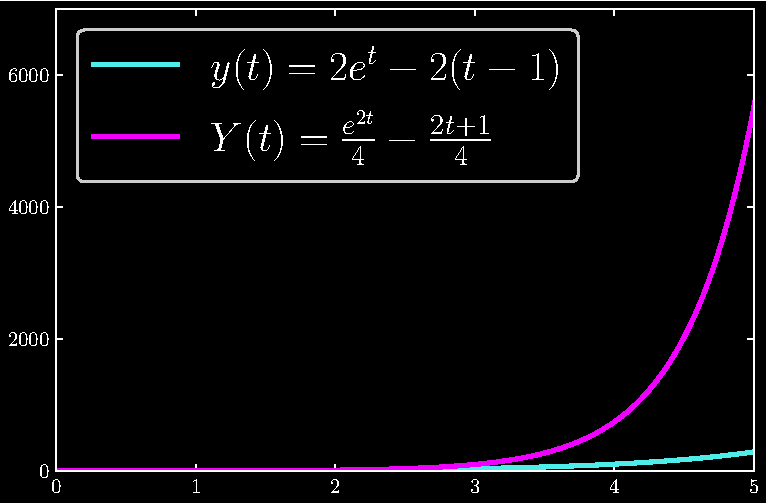
\includegraphics[width=1.0\textwidth]{../chap1/sec1.6/chap1sec1.6ex9.eps}
\end{center}

% QUESTION 10
\qs{1.6.10}{Compare the linear equation \(y' = y\) to the separable equation \(y' = y^{2}\) starting from \(y \!\left( 0 \right) = 1\). Which solution \(y \!\left( t \right) \) must grow faster? It grows so fast that it blows up to \(y \!\left( T \right) = \infty\) at what time \(T\)?}

Solving the equations gives us:

\(\bm{y' = y: }\)
\begin{alignat*}{3}
	&\implies && \frac{d y}{d t} && = y \\
	&\implies && \int^{y \!\left( t \right) }_{y \!\left( 0 \right) } \frac{du}{u}  && = \int^{t}_{0}  \, dt  \\
	&\implies && \ln\left( y \!\left( t \right)  \right) - \ln\left( y \!\left( 0 \right)  \right) && = t \\
	&\implies && y \!\left( t \right) && = e^{t}
\end{alignat*}

\(\bm{y' = y^{2}:}\)
\begin{alignat*}{3}
	&\implies && \frac{d y}{d t} && = y^{2} \\
	&\implies && \int^{y \!\left( t \right) }_{y \!\left( 0 \right) } \frac{du}{u^{2}} && = \int^{t}_{0}  \, dt   \\
	&\implies && \frac{1}{y \!\left( 0 \right) } - \frac{1}{y \!\left( t \right) } && = t \\
	&\implies && y \!\left( t \right) && = \frac{1}{1 - t}
\end{alignat*}

Intuitively, we must have the solution \(y \!\left( t \right) \) to \(y' = y^{2}\) grow faster, assuming that \(y^{2} > y\). But as time approaches \(t = 1\), we see that the solution to \(y' = y^{2}\) hits an asymptotic point, namely
\[
	\lim\limits_{t \to 1} y \!\left( t \right) = \lim\limits_{t \to 1} \frac{1}{1 - t} = \infty
\]

% QUESTION 11
\qs{1.6.11}{\(Y' = 2Y\) has a larger growth factor (because \(a = 2\)) than \(y' = y + q \!\left( t \right) \). What source \(q \!\left( t \right) \) would be needed to keep \(y \!\left( t \right) = Y \!\left( t \right) \) for all time?}

Assume that \(Y \!\left( 0 \right) = y \!\left( 0 \right) \). Solving both equations, we find

\(\bm{Y' = 2Y:}\) Using integrating factor \(e^{-2t}\):
\begin{alignat*}{3}
	&\implies && Y' - 2Y && = 0 \\
	&\implies && \!\left( e^{-2t}Y \right)' && = 0 \\
	&\implies && e^{-2t} Y \!\left( t \right) - Y \!\left( 0 \right) && = 0 \\
	&\implies && Y \!\left( t \right) && = Y \!\left( 0 \right) e^{2t}
\end{alignat*}

\(\bm{y' = y + q \!\left( t \right) :}\) Using integrating factor \(e^{-t}\):
\begin{alignat*}{3}
	&\implies && y' - y && = q \!\left( t \right)  \\
	&\implies && \!\left( e^{-t}y \right)' && = e^{-t}q \!\left( t \right)  \\ 
	&\implies && e^{-t} y \!\left( t \right) - y \!\left( 0 \right) && = \int^{t}_{0} e^{-s}q \!\left( s \right)  \, ds \\
	&\implies && y \!\left( t \right) && = y \!\left( 0 \right) e^{t} + e^{t} \int^{t}_{0} e^{-s}q \!\left( s \right)  \, ds 
\end{alignat*}

For \(y \!\left( t \right) = Y \!\left( t \right) \) for all time \(t\), we need to have
\begin{alignat*}{3}
	&\implies && y \!\left( 0 \right) e^{t} + e^{t} \int^{t}_{0} e^{-s} q \!\left( s \right)  \, ds && = Y \!\left( 0 \right) e^{2t}  \\
	&\implies && \int^{t}_{0} e^{-s} q \!\left( s \right)  \, ds   && = Y \!\left( 0 \right) e^{t} - Y \!\left( 0 \right) \\
	& && && = Y \!\left( 0 \right) \!\left( e^{t} - 1 \right) 
\end{alignat*}
Immediately, we can see that if
\[
	q \!\left( t \right) = Y \!\left( 0 \right) e^{2t}
\]
Then we have the desired equality. We could have also derived this solution by taking our \(Y \!\left( t \right) \) and substituting it into the second equation:
\begin{alignat*}{3}
	&\implies && 2Y \!\left( 0 \right) e^{2t} - Y \!\left( 0 \right) e^{2t} && = q \!\left( t \right)  \\
	&\implies && Y \!\left( 0 \right) e^{2t} && = q \!\left( t \right)  \\ 
\end{alignat*}

% QUESTION 12
\qs{1.6.12}{Starting from \(y \!\left( 0 \right) = Y \!\left( 0 \right) = 1\), does \(y \!\left( t \right) \) or \(Y \!\left( t \right) \) eventually become larger?
\[
	\frac{d y}{d t} = 2y + e^{t} \qquad \frac{d Y}{d t} = Y + e^{2t}.
\]}

\(\bm{\frac{d y}{d t}  = 2y + e^{t}:}\) Using integrating factor \(e^{-2t}\), derive:
\begin{alignat*}{3}
	&\implies && \frac{d y}{d t} - 2y && = e^{t} \\
	&\implies && \!\left( e^{-2t}y \right)' && = e^{-t}  \\
	&\implies && e^{-2t} y \!\left( t \right) - y \!\left( 0 \right) && = \int^{t}_{0} e^{-s} \, ds \\
	&\implies && y \!\left( t \right) && = y \!\left( 0 \right) e^{2t} + e^{2t} \!\left( 1 - e^{-t} \right) \\
	& && && = 2e^{2t} - e^{t}
\end{alignat*}

\(\bm{\frac{d Y}{d t}  = Y + e^{2t}}:\) Using integrating factor \(e^{-t}\), derive:
\begin{alignat*}{3}
	&\implies && \frac{d Y}{d t} - Y && = e^{2t}  \\
	&\implies && \!\left( e^{-t}Y \right)' && = e^{t} \\ 
	&\implies && e^{-t} Y \!\left( t \right) - Y \!\left( 0 \right) && = \int^{t}_{0} e^{s} \, ds \\
	&\implies && Y \!\left( t \right) && = Y \!\left( 0 \right) e^{t} + e^{t} \!\left( e^{t} - 1 \right) \\
	& && && = e^{2t}
\end{alignat*}

Concluding, we see that \(y \!\left( t \right) > Y \!\left( t \right) \) for all time \(t\). We know this since \(e^{2t} > e^{t}\) for all time \(t\), so the subtraction of the \(e^{t}\) term in \(y \!\left( t \right) \) never outpaces the addition of the \(2\) factor on the \(e^{2t}\) term.

\vspace{12pt}

% QUESTION 13
\qs{1.6.13}{What is the factor \(G \!\left( s,s \right) \) in zero time? Find \(G \!\left( s, \infty \right) \) if \(a = -1\) and if \(a = 1\).}

Over zero time, we must have
\[
	G \!\left( s,s \right) = e^{\int^{s}_{s} a \!\left( T \right)  \, dT } = e^{0} = 1
\]
If \(a = -1\), then
\[
	G \!\left( s, \infty \right) = e^{-\int^{\infty}_{s}  \, dT } = 0
\]
And if \(a = 1\), then
\[
	G \!\left( s, \infty \right) = e^{\int^{\infty}_{s}  \, dT } = \infty
\]

% QUESTION 14
\qs{1.6.14}{Explain the important statement after equation (13): \textit{The growth factor \(G \!\left( s, t \right) \) is the solution to \(y' = a \!\left( t \right) y + \delta \!\left( t - s \right) \)}. The source \(\delta \!\left( t - s \right) \) deposits \(\$1\) at time \(s\).}

We solve this equation with integrating factor \(e^{-\int^{t}_{0} a \!\left( T \right)  \, dT }\):
\begin{alignat*}{3}
	&\implies && y' - a \!\left( t \right) y && = \delta \!\left( t - s \right)  \\
	&\implies && \!\left( e^{-\int^{t}_{0} a \!\left( T \right)  \, dT } y \right)' && = e^{-\int^{t}_{0} a \!\left( T \right)  \, dT } \delta \!\left( t - s \right)  \\
	&\implies && e^{-\int^{t}_{0} a \!\left( T \right)  \, dT } y \!\left( t \right) - y \!\left( 0 \right) && = \int^{t}_{0} e^{-\int^{t}_{0} a \!\left( T \right)  \, dT } \delta \!\left( t - s \right)  \, dt \\
	& && && = e^{-\int^{s}_{0} a \!\left( T \right)  \, dT } \\
	&\implies && y \!\left( t \right) && = \!\left( e^{\int^{t}_{0} a \!\left( T \right)  \, dT } \right) \!\left( e^{-\int^{s}_{0} a \!\left( T \right)  \, dT } \right) \\
	& && && = e^{\int^{t}_{s} a \!\left( T \right)  \, dT } \\
	& && && = G \!\left( s,t \right) 
\end{alignat*}

% QUESTION 15
\qs{1.6.15}{Now explain this meaning of \(G \!\left( s,t \right) \) when \(t\) \textit{is less than} \(s\). We go backwards in time. \textit{For} \(t < s\), \(G \!\left( s,t \right) \) \textit{is the value at time }\(t\) \textit{that will grow to equal} \(1\) \textit{at time} \(s\).

\vspace{12pt}

When \(t = 0\), \(G \!\left( s, 0 \right) \) is the ``present value" of a promise to pay \(\$1\) at time \(s\). If the interest rate is \(a = 0.1 = 10\%\) per year, what is the present value \(G \!\left( s,0 \right) \) of a million dollar inheritance promised in \(s = 10\) years?}

When \(t < s\), we necessarily have
\[
	G \!\left( s,t \right) = e^{\int^{t}_{s} a \!\left( T \right)   \, dT } = e^{-\int^{s}_{t} a \!\left( T \right)  \, dT } = \frac{1}{e^{\int^{s}_{t} a \!\left( T \right)  \, dT }}
\]

As \(t \rightarrow s\), \(G \!\left( s, t \right) \rightarrow 1\), and particularly -- the growth factor grows \textit{to} 1 from below. Once \(t = s \), \(G \!\left( s, t \right) = 1\). Intuitively, \(G \!\left( s,t \right) \) simply gives us the portion of the deposit at time \(t < s\); once the time hits \(s\), the deposit has fully grown to the desired amount. 

For the second question, we have
\[
	G \!\left( s,0 \right) = e^{\int^{0}_{s} 0.1 \, dT } = e^{-0.1s}
\]
For \(s = 10\) years, the present value of the million dollar inheritance is
\[
	G \!\left( 10, 0 \right) = \frac{1}{e} \quad \implies \quad 10^{6} G \!\left( 10,0 \right) 
\]

% QUESTION 16
\qs{1.6.16}{\begin{enumerate}[label=(\alph*)]
	\item What is the growth factor \(G \!\left( s,t \right) \) for the equation \(y' = \!\left( \sin t \right) y + Q \sin t\)?
	\item What is the null solution \(y_{n} = G \!\left( 0,t \right) \) to \(y' = \!\left( \sin t \right) y\) when \(y \!\left( 0 \right) = 1\)?
	\item What is the particular solution \(y_{p} = \int^{t}_{0} G \!\left( s,t \right) Q \sin s \, ds  \) ?
\end{enumerate}}

(a) The growth factor is given by
\[
	G \!\left( s,t \right) = \exp\left( \int^{t}_{s} \sin T \, dT  \right) = \exp\left( \cos s - \cos t \right)
\]

(b) The null solution is given by
\begin{alignat*}{3}
	&\implies && y' - \!\left( \sin t \right) y && = 0 \\
	&\implies && \!\left( e^{-\int^{t}_{0} \sin T \, dT } y \right)' && = 0  \\
	&\implies && e^{-\int^{t}_{0} \sin T \, dT } y \!\left( t \right) - y \!\left( 0 \right) && = 0 \\
	&\implies && y_{n} \!\left( t \right) && = e^{\int^{t}_{0} \sin T \, dT } \\
	& && && = e^{1 - \cos t}
\end{alignat*}

Which is equal to
\[
	G \!\left( 0, t \right) = e^{1 - \cos t}
\]

(c) The particular solution is given by the bracketed term:
\begin{alignat*}{3}
	&\implies && y' - \!\left( \sin t \right) y && = Q \sin t \\
	&\implies && \!\left( e^{-\int^{t}_{0} \sin T \, dT }y \right)' && = e^{-\int^{t}_{0} \sin T \, dT } Q \sin t \\ 
	&\implies && e^{-\int^{t}_{0} \sin T \, dT } y \!\left( t \right) - y \!\left( 0 \right) && = \int^{t}_{0} e^{-\int^{s}_{0} \sin T \, dT } Q \sin s \, ds \\ 
	&\implies && y \!\left( t \right) && = e^{1 - \cos t} + \int^{t}_{0} e^{\int^{t}_{s} \sin T \, dT } Q \sin s \, ds \\
	& &&  && = e^{1 - \cos t} + \int^{t}_{0} e^{\cos s - \cos t} Q \sin s \, ds  \\
	& && && = e^{1 - \cos t} + e^{-\cos t} \int^{t}_{0} e^{\cos s} Q \sin s \, ds \\
	& && && = e^{1 - \cos t} + Qe^{-\cos t} \!\left( e - e^{\cos t} \right) \\
	& && && = \underbrace{e^{1 - \cos t}}_{y_{n}} + \underbrace{Q \!\left( e^{1 - \cos t} - 1 \right) }_{y_{p}}
\end{alignat*}

As expected, \(y \!\left( 0 \right) \) gives us \(1\).

\vspace{12pt}

% QUESTION 17
\qs{1.6.17}{\begin{enumerate}[label=(\alph*)]
	\item What is the growth factor \(G \!\left( s,t \right) \) for the equation \(y' = y / \!\left( t + 1 \right) + 10\)? 
	\item What is the null solution \(y_{n} = G \!\left( 0,t \right) \) to \(y' = y / \!\left( t + 1 \right) \) with \(y \!\left( 0 \right) = 1\)?
	\item What is the particular solution \(y_{p} = 10 \int^{t}_{0} G \!\left( s,t \right)  \, ds  \)?
\end{enumerate}}

(a) The growth factor \(G \!\left( s,t \right) \) is given by
\begin{align*}
	G \!\left( s,t \right) &= \exp\left( \int^{t}_{s} \frac{1}{T + 1} \, dT \right) \\
			       & = \exp\left( \ln\left( t + 1 \right) - \ln\left( s + 1 \right) \right) \\
			       & = \exp\left( \ln\left( \frac{t + 1}{s + 1} \right) \right) \\
			       & = \frac{t + 1}{s + 1}
\end{align*}

(b) We derive the null solution as
\begin{alignat*}{3}
	&\implies && y' - \frac{y}{t + 1} && = 0 \\
	&\implies && \!\left( e^{-\int^{t}_{0} 1 / \!\left( T + 1 \right)  \, dT } y \right)' && = 0  \\ 
	&\implies && e^{-\int^{t}_{0} 1 / \!\left( T + 1 \right)  \, dT } y \!\left( t \right) - y \!\left( 0 \right) && = 0 \\
	&\implies && y_{n} \!\left( t \right) && = e^{\int^{t}_{0} 1 / \!\left( T + 1 \right)  \, dT } \\
	& && && = t + 1 
\end{alignat*}

Which is equal to
\[
	G \!\left( 0, t \right) = t + 1
\]

(c) The particular solution is given in brackets
\begin{alignat*}{3}
	&\implies && y' - \frac{y}{t + 1} && = 10 \\
	&\implies && \!\left( e^{-\int^{t}_{0} 1 / \!\left( T + 1 \right)  \, dT } y \right)' && = 10 e^{-\int^{t}_{0} 1 / \!\left( T + 1 \right)  \, dT } \\ 
	&\implies && e^{-\int^{t}_{0} 1 / \!\left( T + 1 \right)  \, dT } y \!\left( t \right) - y \!\left( 0 \right) && = \int^{t}_{0} \frac{10}{s + 1} \, ds \\
	&\implies && y \!\left( t \right) && = \underbrace{t + 1}_{y_{n}} + \underbrace{10 \!\left( t + 1 \right) \ln\left( t + 1 \right)}_{y_{p}}
\end{alignat*}

\vspace{12pt}

As expected, \(y \!\left( 0 \right) \) yields \(1\).

\vspace{12pt}

% QUESTION 18
\qs{1.6.18}{Why is \(G \!\left( t, s \right) = 1 / G \!\left( s, t \right) \)? Why is \(G \!\left( s, t \right) = G \!\left( s, S \right) G \!\left( S, t \right) \)?}

By definition,
\[
	G \!\left( t,s \right) = \exp\left( \int^{s}_{t} a \!\left( T \right)  \, dT  \right)
\]
By the Fundamental Theorem of Calculus, flipping the bounds of integration changes the sign of the integral:
\begin{align*}
	G \!\left( t,s \right) & = \exp\left( \int^{s}_{t} a \!\left( T \right)  \, dT  \right) \\
		 & = \exp\left( -\int^{t}_{s} a \!\left( T \right)  \, dT  \right) \\
		 & = 1 / \exp\left( \int^{t}_{s} a \!\left( T \right)  \, dT  \right) \\
		 & = 1 / G \!\left( s, t \right)  
\end{align*}

Secondly, suppose that \(s \le S \le t\). Then
\begin{align*}
	G \!\left( s, t \right)  & = \exp\left( \int^{t}_{s} a \!\left( T \right) \, dT  \right) \\
	 & = \exp\left( \int^{S}_{s} a \!\left( T \right)  \, dT + \int^{t}_{S} a \!\left( T \right)  \, dT  \right)  \\
	 & = \exp\left( \int^{S}_{s} a \!\left( T \right)  \, dT  \right) \exp\left( \int^{t}_{S} a \!\left( T \right)  \, dT  \right) \\
	 & = G \!\left( s, S \right) G \!\left( S, t \right) 
\end{align*}

% QUESTION 19	
\qs{1.6.19}{(recommended) If \(dy / dt = ay + qe^{i \omega t}\), with \(t\) in seconds and \(y\) in meters, what are the units for \(a\) and \(q \) and \(\omega \)?}

The units for \(a\), \(q \), and \(\omega \) are in \(1 / \text{s}\), \(m/s\), and \(1/s\), respectively. We have \(a\) and \(q \) as frequencies, and \(q \) is velocity.

\vspace{12pt}

% QUESTION 20
\qs{1.6.20}{The logistic equation \(dy / dt = ay - by^{2}\) often measures the time \(t\) in years (and \(y\) counts people). What are the units of \(a\) and \(b\)?}

The units for \(a\) and \(b\) are \(1 / \text{year}\) and \(1 / \!\left( \text{people} \cdot \text{year} \right) \), respectively.

\vspace{12pt}

% QUESTION 21
\qs{1.6.21}{Newton's Law is \(m \frac{d^{2} y}{d t^{2}} + ky = F \). If the mass \(m\) is in grams, \(y\) is in meters, and \(t\) is in seconds, what are the units of the stiffness \(k\) and the force \(F\)?}

The units for \(k\) and \(F\) are \(g / s^{2}\) and \(g \cdot m / s^{2}\), respectively.

\vspace{12pt}

% QUESTION 22
\qs{1.6.22}{Why is our favorite example \(y' = y + 1\) very unsatisfactory dimensionally? Solve it anyway starting from \(y \!\left( 0 \right) = -1\) and from \(y \!\left( 0 \right) = 0\).}

We have \(y'\) represented in units of something per unit time, while \(y\) is in units of something, and ambiguity as to the unit of the constant \(1\). Nevertheless, we solve it using the integrating factor \(e^{-t}\):
\begin{alignat*}{3}
	&\implies && y' - y && = 1 \\
	&\implies && \!\left( e^{-t}y \right)' && = e^{-t} \\ 
	&\implies && e^{-t} y \!\left( t \right) - y \!\left( 0 \right) && = \int^{t}_{0} e^{-s} \, ds \\
	&\implies && y \!\left( t \right) && = -e^{t} + e^{t} \!\left(-e^{-t} + 1  \right) \\
	& && && = -1
\end{alignat*}

% QUESTION 23
\qs{1.6.23}{The difference equation \(Y_{n+1} = cY_{n} + Q_{n}\) produces \(Y_{1} = cY_{0} + Q_{0}\). Show that the next step produces \(Y_{2} = c^{2} Y_{0} + cQ_{0} + Q_{1}\). After \(N\) steps, the solution formula for \(Y_{N}\) is like the solution formula for \(y' = ay + q \!\left( t \right) \). Exponentials of \(a\) change to powers of \(c\), the null solution \(e^{at} y \!\left( 0 \right) \) becomes \(c^{N} Y_{0}\). The particular solution
\[
	Y_{N} = c^{N - 1} Q_{0} + \cdots + Q_{N - 1} \quad \text{is like} \quad y \!\left( t \right) = \int^{t}_{0} e^{a \!\left( t-s \right) q \!\left( s \right) } \, ds. 
\]}

By definition, we have
\begin{align*}
	Y_{2} & = cY_{1} + Q_{1} \\
	     & = c \!\left( c Y_{0} + Q_{0} \right) + Q_{1} \\ 
	     & = c^{2} Y_{0} + cQ_{0} + Q_{1}
\end{align*}

Moving onto \(Y_{3}\), we can derive
\begin{align*}
	Y_{3} & = cY_{2} + Q_{2} \\
	 & = c \!\left( c^{2}Y_{0} + cQ_{0} + Q_{1} \right)  \\ 
	 & = c^{3}Y_{0} + c^{2}Q_{0} + cQ_{1} + Q_{2}
\end{align*}

By now, a pattern emerges, from which we can conjecture that \(Y_{N}\) is of form
\[
	Y_{N} = \underbrace{c^{N} Y_{0}}_{y_{n}} + \underbrace{\sum_{i=0}^{N-1} c^{N - 1 - i}Q_{i}}_{y_{p}}
\]

% QUESTION 24
\qs{1.6.24}{Suppose a fungus doubles in size every day, and it weighs a pound after 10 days. If another fungus was twice as large at the start, would it weigh a pound in 5 days?}

By premise, we must have
\[
	y \!\left( t \right) = C2^{t}
\]
where \(t\) is in units of days. Since \(y \!\left( 10 \right) = 1\), the constant \(C\) must equal
\[
	C = \frac{1}{2^{10}}
\]
So at \(t = 0\), the fungus must be \(1 / 2^{10}\) pounds. Suppose now the second fungus starts at size \(2 / 2^{10} = 1 / 2^{9}\). Then when \(t = 9\), we have
\[
	y \!\left( 9 \right) = \frac{1}{2^{9}} \cdot 2^{9} = 1
\]
Thus it would take 9 days for the second fungus that is twice as large as the first to grow to one pound.

\newpage
\subsection{\textsf{1.7 - The Logistic Equation}}
% QUESTION 1
\qs{1.7.1}{If \(y \!\left( 0 \right) = a/2b\), the halfway point on the \(S\)-curve is at \(t = 0\). Show that \(d = b\) and \(y \!\left( t \right) = \displaystyle{\frac{a}{de^{-at} + b} = \frac{a}{b} \frac{1}{e^{-at} + 1}}\). Sketch the curve from \(y_{-\infty} = 0\) to \(y_{\infty} = \displaystyle{\frac{a}{b}}\).}

Given the logistic equation
\[
	\frac{d y}{d t} = ay - by^{2}
\]
We let \(z = 1/y\), implying that
\[
	\frac{d z}{d t} = -\frac{1}{y^{2}} \frac{d y}{d t} 
\]
Thus we can rewrite the logistic equation as
\[
	\frac{d z}{d t} = -\frac{1}{y^{2}} \!\left( ay - by^{2} \right) = - \!\left( \frac{a}{y} - b \right) = -az + b
\]
which has solution
\begin{alignat*}{3}
	&\implies && \frac{d z}{d t}  + az && = b \\
	&\implies && \!\left( e^{at}z \right)' && = b e^{at} \\ 
	&\implies && e^{at} z \!\left( t \right) - z \!\left( 0 \right) && = \int^{t}_{0} be^{at} \, dt \\
	& && && = \frac{b}{a} \!\left( e^{at} - 1 \right)  \\
	&\implies && z \!\left( t \right) && = e^{-at} z \!\left( 0 \right) + \frac{b}{a} \!\left( 1 - e^{-at} \right) 
\end{alignat*}

Now let \(d/a = z \!\left( 0 \right) - b/a\). Since \(z \!\left( 0 \right) = 1/y \!\left( 0 \right) \), we have \(d = a / y \!\left( 0 \right) - b\). Then we may write
\[
	z \!\left( t \right) = \frac{d e^{-at} + b}{a}
\]
Finally implying
\[
	y \!\left( t \right) = \frac{a}{de^{-at} + b}
\]
Now, for \(\displaystyle{y \!\left( 0 \right) = \frac{a}{2b}}\), our parameter \(d\) is
\[
	d = \frac{a}{a / 2b} - b = 2b - b = b
\]
enabling us to conclude
\[
	y \!\left( t \right) = \frac{a}{b} \frac{1}{e^{-at} + 1}
\]
The curve is graphed as

\begin{center}
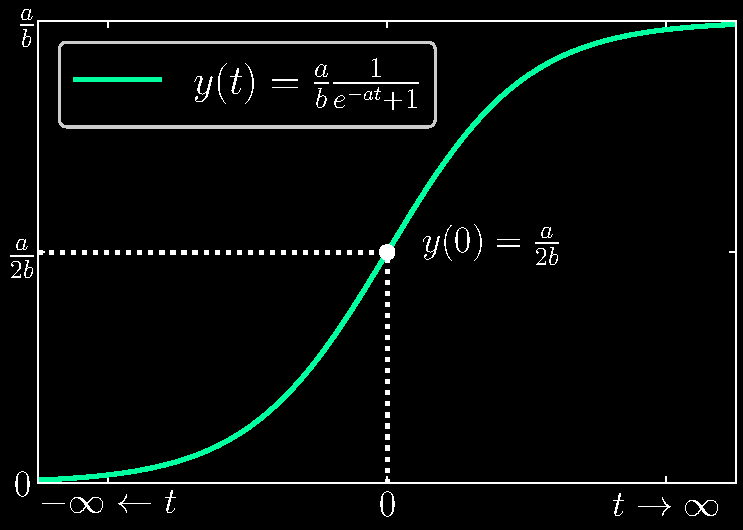
\includegraphics[width=1.0\textwidth]{../chap1/sec1.7/chap1sec1.7ex1.eps}
\end{center}

% QUESTION 2
\qs{1.7.2}{If the carrying capacity of the Earth is \(K = a/b = 14\) billion people, what will be the population at the inflection point? What is \(dy/dt\) at that point? The actual population was 7.14 billion on January 1, 2014.}

The inflection point is at \(y \!\left( t \right) = a / 2b\), or
\[
	y \!\left( t \right) = \frac{a}{2b} = 7 \text{ billion people}
\]
The natural growth rate \(a\) is estimated to be \(.029\) per year. Then we have
\[
	b = \frac{a}{K} = \frac{.029}{14 \cdot 10^{9}} \approx 2.1 \cdot 10^{-12}
\]
which corresponds to \(dy/dt\):
\[
	\frac{d y}{d t} = 0.029 \!\left( 7 \cdot 10^{9} \right)  - \!\left( 2.1 \cdot 10^{-12} \right) \!\left( 7 \cdot 10^{9} \right)^{2} \approx 10^{8} 
\]

% QUESTION 3
\qs{1.7.3}{Equation (18) must give the same formula for the solution \(y \!\left( t \right) \) as equation (16). If the right side of (18) is called \(R\), we can solve that equation for \(y\):
\[
	y = R \!\left( 1 - \frac{b}{a}y \right) \quad \rightarrow \quad \!\left( 1 + R \frac{b}{a} \right) y = R \quad \rightarrow \quad y = \frac{R}{\!\left( 1 + R \frac{b}{a} \right) }
\]
Simplify that answer by algebra to recover equation (16) for \(y \!\left( t \right) \).}

Equation (18) is given by
\[
	\frac{y}{1 - \frac{b}{a}y} = e^{at} \frac{y \!\left( 0 \right) }{1 - \frac{b}{a} y \!\left( 0 \right) } = R
\]

Which we solve by
\begin{alignat*}{2}
	\implies && y & = R \!\left( 1 - \frac{b}{a}y \right)  \\
	\implies && \!\left( 1 + R \frac{b}{a} \right) y & = R \\ 
	\implies && y & = \frac{R}{\!\left( 1 + R \frac{b}{a} \right) } 
\end{alignat*}

Now, define \(d\) as
\[
	d = \frac{a}{y \!\left( 0 \right) - b}
\]
Then we may write \(R\) as
\[
	R = e^{at} \!\left( \frac{a}{d} \right) 
\]
which is more compact to work with. Then we continue with
\begin{alignat*}{3}
	\implies && y & = \frac{e^{at} \!\left( \frac{a}{d} \right) }{1 + \!\left( \frac{b}{a} \right) e^{at} \!\left( \frac{a}{d} \right) } \\
	\implies && y & = \frac{e^{at} \!\left( \frac{a}{d} \right) }{\!\left( d + be^{at} \right) / d}  \\ 
	\implies && y & = \frac{ae^{at}}{d + be^{at}} \\
	\implies && y & = \frac{a}{de^{-at} + b}
\end{alignat*}

Deriving the desired result, equation (16).

\vspace{12pt}

% QUESTION 4
\qs{1.7.4}{Change the logistic equation to \(y' = y + y^{2}\). Now the nonlinear term is positive, and \textit{cooperation of} \(y\) \textit{with} \(y\) promotes growth. Use \(z = 1/y\) to find and solve a linear equation for \(z\), starting from \(z \!\left( 0 \right) = y \!\left( 0 \right) = 1\). Show that \(y \!\left( T \right) = \infty\) when \(e^{-T} = 1/2\). Cooperation looks bad, the population will explode at \(t = T\).}

Given \(y' = y + y^{2}\), let \(z = 1/y\). Then
\begin{alignat*}{3}
	\implies && z' & = -\frac{1}{y^{2}}y' \\
	&& & = -\frac{1}{y} - 1 \\ 
	&& & = - \!\left( z + 1 \right) 
\end{alignat*}

Writing \(z'\) as \(\displaystyle{\frac{d z}{d t} }\) and separating variables, we can write

\begin{alignat*}{2}
	\implies && \frac{d z}{d t}  & = - \!\left( z + 1 \right)  \\
	\implies && - \int^{z \!\left( t \right) }_{z \!\left( 0 \right) } \frac{dz}{z + 1}  & = \int^{t}_{0} \, dt  \\ 
	\implies && -\ln\left( z \!\left( t \right) + 1 \right) + \ln\left( 2 \right) & = t \\
	\implies && \ln\left( \frac{2}{z \!\left( t \right)  + 1} \right) & = t \\
	\implies && \frac{2}{z \!\left( t \right) + 1} & = e^{t} \\
	\implies && z \!\left( t \right) & = 2e^{-t} - 1 \\
	\implies && y \!\left( t \right) & = \frac{1}{2e^{-t} - 1}
\end{alignat*}

Clearly, we have \(z \!\left( 0 \right) = y \!\left( 0 \right) = 1\). Now, suppose that we have
\[
	\lim\limits_{T \to \ln\left( 2 \right)} e^{-T} = \frac{1}{2}
\]
Then it must follow that
\[
	\lim\limits_{T \to \ln\left( 2 \right)}  y \!\left( t \right) = \lim\limits_{T \to \ln\left( 2 \right)} \frac{1}{2e^{-t} - 1} = \infty
\]
Which indicates an explosion of population as \(T\) approaches \(\ln\left( 2 \right)\).

\vspace{12pt}

% QUESTION 5
\qs{1.7.5}{The US population grew from 313,873,685 in 2012 to 316,128,839 in 2014. If it were following a logistic \(S\)-curve, what equations would give you \(a\), \(b\), \(d\) in the formula (4)? Is the logistic equation reasonable and how to account for immigration?}

Suppose we set \(t = 0\) as corresponding to 2012. Then \(t = 2\) corresponds to 2014. We have
\[
	y \!\left( 0 \right) = \frac{a}{d + b} = 313,873,685 \quad \text{and} \quad y \!\left( 2 \right) = \frac{a}{de^{-2a} + b} = 316,128,839
\]
Due to the nonlinearity, it is not readily clear how we identify the corresponding logistic equation that fits these points. As far as immigration goes, suppose we add the constant harvesting rate \(-h\) to the logistic equation:
\[
	\frac{d y}{d t} = ay - by^{2} - h
\]
Since immigration would lead to an \textit{increase} in \(dy/dt\), we must have \(h < 0\). By contrast, \textit{emigration decreases} \(dy/dt\), corresponding to \(h > 0\).

\vspace{12pt}

% QUESTION 6
\qs{1.7.6}{The \textbf{Bernoulli equation} \(y' = ay - by^{n}\) has competition term \(by^{n}\). Introduce \(z = y^{1-n}\) which matches the logistic case when \(n = 2\). Follow equation (4) to show that \(z' = \!\left( n - 1 \right) \!\left( -az + b \right) \). Write \(z \!\left( t \right) \) as in (5)-(6). Then you have \(y \!\left( t \right) \).}

Let \(z = y^{1-n}\). Then we have
\[
	z' = \!\left( 1-n \right) y^{-n} y'
\]

and are able to derive
\begin{alignat*}{2}
	\implies && z' & = \!\left( 1 - n \right) \!\left(ay^{1-n} - b\right) \\
	&& & = \!\left( n - 1 \right) \!\left( -az + b \right)
\end{alignat*}
Separating variables, we can conclude with
\begin{alignat*}{2}
	\implies && \frac{d z}{d t}  & = \!\left( n - 1 \right) \!\left( -az + b \right)  \\
	\implies && \int^{z \!\left( t \right) }_{z \!\left( 0 \right) } \frac{dz}{-az + b}  & = \int^{t}_{0} \!\left( n - 1 \right)  \, dt  \\ 
	\implies && -\frac{1}{a} \!\left( \ln\left( -az \!\left( t \right) + b \right) - \ln\left( -a z \!\left( 0 \right) + b \right) \right) & = \!\left( n - 1 \right) t \\
	\implies && \frac{-a z \!\left( t \right) + b}{-a z \!\left( 0 \right) + b} & = e^{-a \!\left( n - 1 \right) t} \\
	\implies && z \!\left( t \right) & = -\frac{1}{a} \!\left( \!\left( -a z \!\left( 0 \right) + b \right) e^{a \!\left( 1 - n \right) t} - b \right) \\ 
		 && & = z \!\left( 0 \right) e^{a \!\left( 1 - n \right) t} - \frac{b}{a} \!\left( e^{a \!\left( 1 - n \right) t} - 1 \right) 
\end{alignat*}

Now, define \(d\) as
\[
	d = \frac{a}{y \!\left( 0 \right) } - b
\]
Then we have
\[
	z \!\left( t \right) = \frac{de^{a \!\left( 1 - n \right) t} + b}{a}
\]
Finally implying
\[
	y \!\left( t \right) = \frac{a}{de^{-a \!\left( n - 1 \right) t} + b}
\]

% QUESTION 7
\qs{1.7.7}{\(y' = y - y^{2}\) is solved by \(y \!\left( t \right) = 1 / \!\left( de^{-t} + 1 \right) \). This is an \(S\)-curve when \(y \!\left( 0 \right) = 1/2\) and \(d = 1\). But show that \(y \!\left( t \right) \) is very different if \(y \!\left( 0 \right) > 1\) or if \(y \!\left( 0 \right) < 0\).

If \(y \!\left( 0 \right) = 2\) then \(d = \frac{1}{2} - 1 = -\frac{1}{2}\). Show that \(y \!\left( t \right) \rightarrow 1\) from above.

If \(y \!\left( 0 \right) = -1\) then \(d = \frac{1}{-1} - 1 = -2\). At what time \(T\) is \(y \!\left( T \right) = -\infty\)?}

Suppose that \(y \!\left( 0 \right) > 1\). Then we have
\[
	d = \frac{1}{y \!\left( 0 \right) } - 1 < 0
\]
We can also determine that \(y \!\left( 0 \right) < 0\) leads to the same result: \(d\) \textit{is negative.} When \(d\) is negative, then we have a discontinuity at \(t\) when \(de^{-t} + 1 = 0\). The \(S\)-curve has no such discontinuity, so there is a stark difference when the initial condition \(y \!\left( 0 \right) \) meets the aforementioned values.

Suppose that \(y \!\left( 0 \right) = 2\). Then \(d = -1/2\). The steady state is \(a/b = 1/1 = 1\). We have
\[
	\lim\limits_{t \to \infty} \frac{1}{-\frac{1}{2}e^{-t} + 1} = 1
\]

and \(y \!\left( t \right) \) approaches 1 from above.

\begin{center}
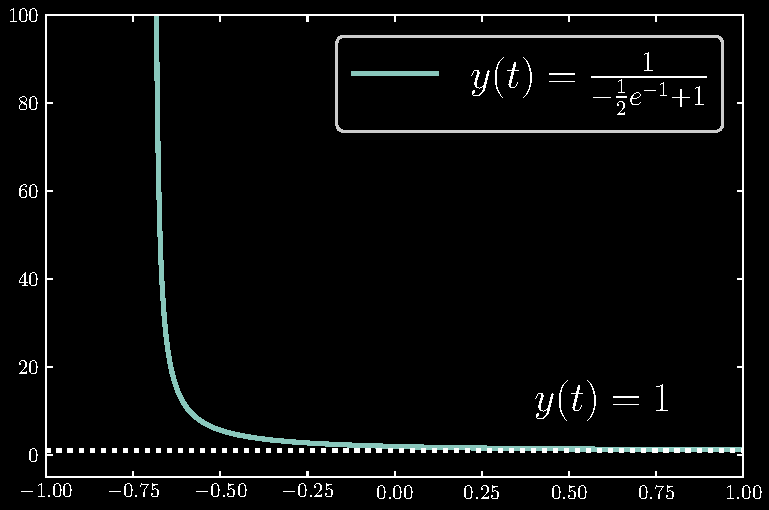
\includegraphics[width=1.0\textwidth]{../chap1/sec1.7/chap1sec1.7ex7a.eps}
\end{center}

In the case where \(y \!\left( 0 \right) = -1\), then \(d = -2\). 
\[
	y \!\left( t \right) = \frac{1}{-2e^{-t} + 1}
\]
The point where approaching \(t = T\) corresponds to \(y \!\left( t \right) \) tending towards \(-\infty\) is where the denominator approaches zero. This time \(t = T\) is thus at
\begin{alignat*}{2}
	\implies && -2e^{-T} + 1 & = 0 \\
	\implies && e^{-T} & = \frac{1}{2} \\ 
	\implies && T & = -\ln\left( \frac{1}{2} \right) \\
		 && & = \ln\left( 2 \right)
\end{alignat*}

\begin{center}
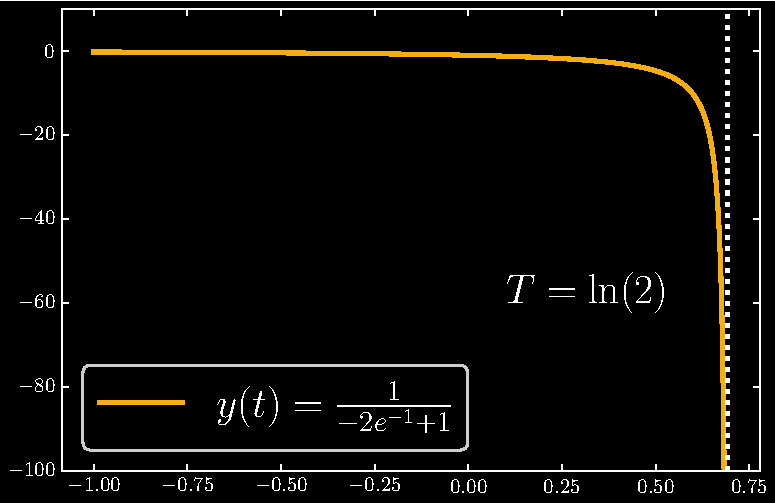
\includegraphics[width=1.0\textwidth]{../chap1/sec1.7/chap1sec1.7ex7b.eps}
\end{center}

% QUESTION 8
\qs{1.7.8}{(recommended) Show those 3 solutions to \(y' = y - y^{2}\) in one graph! They start from \(y \!\left( 0 \right) = 1/2\) and 2 and \(-1\). The \(S\)-curve climbs from \(\frac{1}{2}\) to 1. Above that, \(y \!\left( t \right) \) descends from 2 to 1. Below the \(S\)-curve, \(y \!\left( t \right) \) drops from \(-1\) to \(-\infty\).

Can you see 3 regions in the picture? \textbf{Dropin curves above \(\bm{y = 1}\) and \(\bm{S}\)-curves sandwiched between 0 and 1 and dropoff curves below \(\bm{y = 0}\).}}

For the given initial conditions, we have solutions
\begin{align*}
	d_{1} & = \frac{1}{1/2} - 1 = 1 \\
	y_{1} \!\left( t \right)  & = \frac{1}{e^{-t} + 1} \\
	d_{2} & = \frac{1}{2} - 1 = -\frac{1}{2} \\
	y_{2} \!\left( t \right) & = \frac{1}{\!\left( -1/2 \right) e^{-t} + 1} \\
	d_{3} & = \frac{1}{-1} - 1 = -2 \\
	y_{3} & = \frac{1}{-2e^{-t} + 1}
\end{align*}

The functions we graph as
\begin{center}
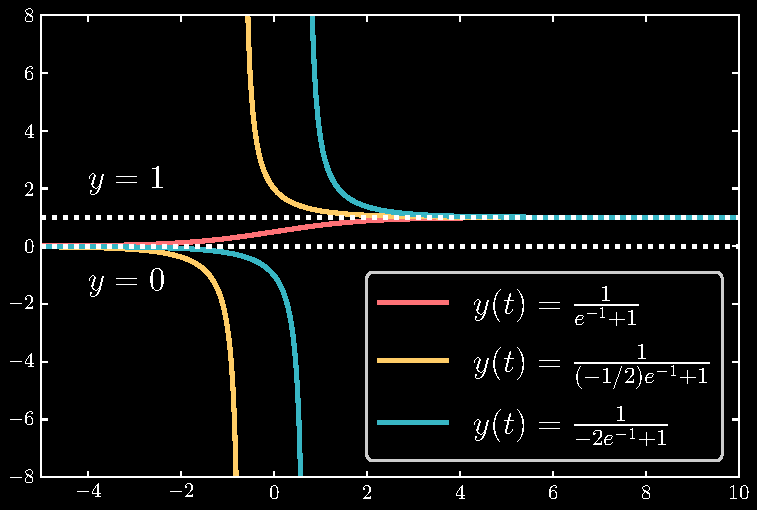
\includegraphics[width=1.0\textwidth]{../chap1/sec1.7/chap1sec1.7ex8.eps}
\end{center}

The \(S\)-curve falls within the interval \(y \in \left( 0, \displaystyle{\frac{a}{b} = 1} \right) \), and when the initial conditions fall outside of that range, we end up with dropin and dropout curves that asymptotically approach the bounds of the interval.

\vspace{12pt}

% QUESTION 9
\qs{1.7.9}{Graph \(f \!\left( y \right) = y - y^{2}\) to see the unstable steady state \(Y  = 0\) and the stable \(Y = 1\). Then graph \(f \!\left( y \right) = y - y^{2} - 2/9\) with harvesting \(h = 2/9\). What are the steady states \(Y_{1}\) and \(Y_{2}\)? The 3 regions in Problem 8 now have \(Z\)-curves above \(y = 2/3\), \(S\)-curve sandwiched between \(1/3\) and \(2/3\), dropoff curves below \(y = 1/3\).}

For the harvesting equation, we have steady states
\[
	Y_{1}, Y_{2} = \frac{-1 \pm \sqrt{1 - 8/9}}{-2} = \frac{1}{3}, \frac{2}{3} 
\]
Allowing for the decomposition
\[
	f \!\left( y \right) = y - y^{2} - 2/9 = \!\left( Y_{1} - \frac{1}{3} \right) \!\left( Y_{2} - \frac{2}{3} \right) = 0
\]
At these steady states, we have
\[
	\frac{d f}{d y} = 1 - 2y; \frac{d f}{d y} \!\left(Y_{1} = \frac{1}{3} \right) = \frac{1}{3} \quad \text{and} \quad \frac{d f}{d y} \!\left(Y_{2} = \frac{2}{3} \right) = -\frac{1}{3}
\]
Concluding that \(Y_{1}\) is an \textbf{unstable} steady state and \(Y_{2}\) is a \textbf{stable} steady state. 

Graphically, we have

\begin{center}
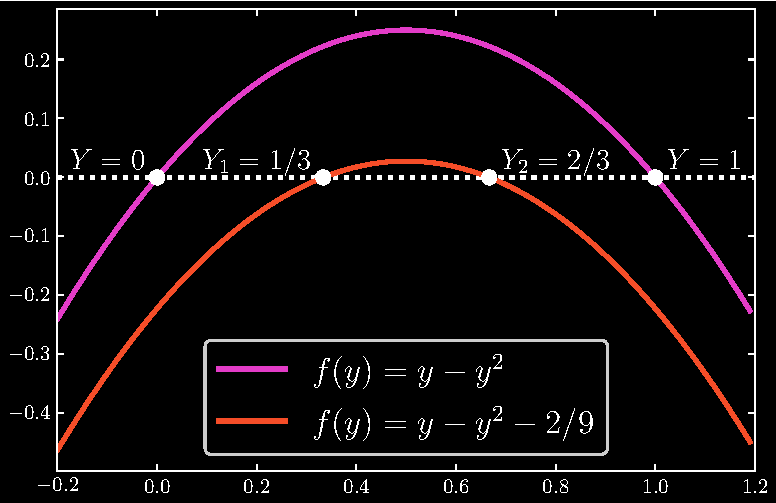
\includegraphics[width=1.0\textwidth]{../chap1/sec1.7/chap1sec1.7ex9.eps}
\end{center}

% QUESTION 10
\qs{1.7.10}{What equation produces an \(S\)-curve climbing to \(y_{\infty} = K\) from \(y_{-\infty} = L\)?}

Our steady states are \(y_{\infty}, y_{-\infty} = K, L\). Then for the general equation \(f \!\left( y \right) = ay - by^{2} - h\), we must have
\begin{align*}
	aK - bK^{2} - h & = 0 \\
	aL - bL^{2} - h & = 0 
\end{align*}
Which simply screams matrix algebra to identify the unknown \(a\) and \(b\) parameters for a given harvesting term \(h\). We set up our matrix equation as such:
\[
	\underbrace{\begin{bmatrix}
		K & -K^{2} \\
		L & -L^{2} \\
\end{bmatrix}}_{A}
\begin{bmatrix}
	a \\
	b \\
\end{bmatrix}
=
\begin{bmatrix}
	h \\
	h \\
\end{bmatrix}
\]
Now, we have determinant
\[
	\det A = -KL^{2} + LK^{2} = LK \!\left( K - L \right) 
\]
which yields the inverse matrix
\[
	A^{-1} = \frac{1}{LK \!\left( K - L \right) }
	\begin{bmatrix}
		-L^{2} & K^{2} \\
		-L & K \\
	\end{bmatrix}
\]
Lastly, we find \(a\) and \(b\) to be
\[
	\begin{bmatrix}
		a \\
		b \\
	\end{bmatrix}
= \frac{1}{LK \!\left( K - L \right) }
\begin{bmatrix}
	-L^{2} & K^{2} \\
	-L & K \\
\end{bmatrix}
\begin{bmatrix}
	h \\
	h \\
\end{bmatrix}
\]
\begin{align*}
	a & = \frac{h}{LK \!\left( K - L \right) } \!\left( K^{2} - L^{2} \right)  \\
	 & = h \!\left( \frac{K + L}{KL} \right)  \\
	 & = \boxed{h \!\left( \frac{1}{K} + \frac{1}{L} \right)} \\
	b & = \frac{h}{LK \!\left( K - L \right) } \!\left( K - L \right) \\
	  & = \boxed{\frac{h}{KL}}
\end{align*}

% QUESTION 11
\qs{1.7.11}{\(y' = y - y^{2} - \frac{1}{4} = - \!\left( y - \frac{1}{2} \right)^{2}\) shows \textit{critical harvesting} with a double steady state at \(y = Y = \frac{1}{2}\). The layer of \(S\)-curves shrinks to that single line. Sketch a dropin curve that starts above \(y \!\left( 0 \right) = \frac{1}{2}\) and a dropoff curve that starts below \(y \!\left( 0 \right) = \frac{1}{2}\).}

Let's solve this equation. By separable variables, we find

\begin{alignat*}{3}
	\implies && \frac{d y}{d t}  & = y - y^{2} - \frac{1}{4} \\
	\implies && \int^{y \!\left( t \right) }_{y \!\left( 0 \right) } -\frac{dy}{\!\left( y - 1/2 \right)^{2}}  & = \int^{t}_{0}  \, dt  \\ 
	\implies && \frac{1}{y \!\left( t \right) - 1/2} - \frac{1}{y \!\left( 0 \right) - 1/2} & = t \\
	\implies && \frac{1}{y \!\left( t \right) - 1/2} & = t + \frac{1}{y \!\left( 0 \right) - 1/2} \\
	\implies && 1 & = \!\left( y \!\left( t \right) - 1/2 \right) \!\left( t + \frac{1}{y \!\left( 0 \right) - 1/2} \right) \\
	\implies && y \!\left( t \right) & = \frac{y \!\left( 0 \right) - 1/2}{y \!\left( 0 \right) t - t/2 + 1} + \frac{1}{2} \\
\end{alignat*}

From here, we may deduce that \(y \!\left( 0 \right) = 1/2\) implies
\[
	y \!\left( t \right) = \frac{1}{2}
\]
as expected. In other words, the ``\(S\)''-curve collapses into a horizontal line at the point of critical harvesting.

Suppose that we have cases in which \(y \!\left( 0 \right) = 1\) and \(y \!\left( 0 \right) = 0\). Then we can graph dropin and dropoff curves:

\begin{center}
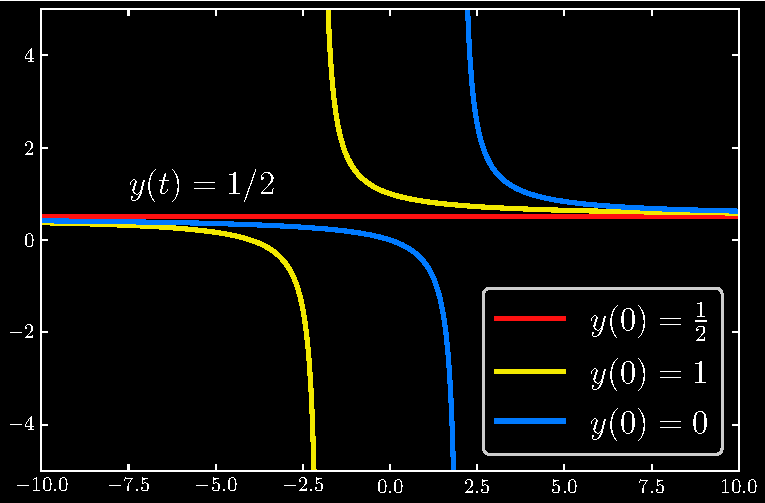
\includegraphics[width=1.0\textwidth]{../chap1/sec1.7/chap1sec1.7ex11.eps}
\end{center}

% QUESTION 12
\qs{1.7.12}{Solve the equation \(y' = -\!\left( y - \frac{1}{2} \right)^{2}\) by substituting \(v = y - \frac{1}{2}\) and solving \(v' = -v^{2}\).}

See 1.7.11.

\vspace{12pt}

% QUESTION 13
\qs{1.7.13}{With overharvesting, every curve \(y \!\left( t \right) \) drops to \(-\infty\). There are no steady states. Solve \(Y - Y^{2} - h= 0\) (quadratic formula) to find only complex roots if \(4h > 1\).

The solutions for \(h = \frac{5}{4}\) are \(y \!\left( t \right) = \frac{1}{2} - \tan \!\left( t + C \right) \). Sketch that dropoff if \(C = 0\). Animal populations don't normally collapse like this from overharvesting.}

By the quadratic formula, we have

\[
	Y = -\frac{1 \pm \sqrt{1 - 4h}}{2}
\]
which leads to complex roots if \(4h > 1\). To solve this equation, we rewrite \(y - y^{2} - 5/4\) as
\[
	y - y^{2} - \frac{5}{4} = -\!\left( y - \frac{1}{2} \right)^{2} - 1
\]
We then solve the equation

\begin{alignat*}{3}
	\implies && \frac{d y}{d t}   & = - \!\left( y - \frac{1}{2} \right)^{2} - 1 \\
	\implies && -\int^{y \!\left( t \right) }_{y \!\left( 0 \right) } \frac{dy}{\!\left( y - 1/2 \right)^{2} + 1}  & = \int^{t}_{0}  \, dt  \\ 
	\implies && \tan^{-1} \!\left( y \!\left( 0 \right) - \frac{1}{2} \right) - \tan^{-1} \!\left( y \!\left( t \right) - \frac{1}{2} \right) & = t
\end{alignat*}

Now let \(\tan^{-1} \!\left( y \!\left( 0 \right) - \frac{1}{2} \right) \) be a constant \(C\). We have

\begin{alignat*}{3}
	\implies && \tan^{-1} \!\left( y \!\left( t \right) - \frac{1}{2} \right)  & - \!\left( t + C \right)  \\
	\implies && y \!\left( t \right) - \frac{1}{2} & = \tan \!\left( - \!\left( t + C \right)  \right)  \\ 
	\implies && y \!\left( t \right) & = \frac{1}{2} - \tan \!\left( t + C \right) 
\end{alignat*}

Graphically, if \(C = 0\), we have \(y \!\left( 0 \right) = \frac{1}{2}\). At \(\displaystyle{t = \frac{\pi }{2}}\), we have \(\displaystyle{y \!\left( \frac{\pi }{2} \right) = 0}\).

\begin{center}
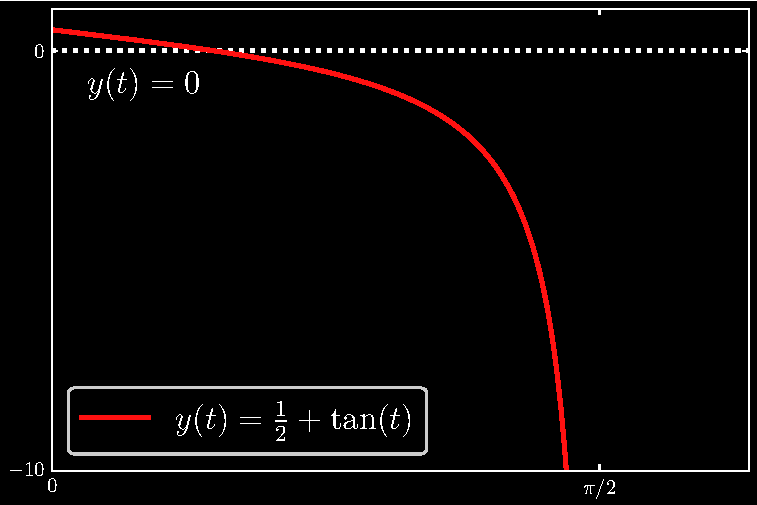
\includegraphics[width=1.0\textwidth]{../chap1/sec1.7/chap1sec1.7ex13.eps}
\end{center}

\newpage
% QUESTION 14
\qs{1.7.14}{With \textbf{two partial fractions}, this is my preferred way to find \(\displaystyle{A = \frac{1}{r - s}}\), \(\displaystyle{B = \frac{1}{s - r}}\)
\[
	\boxed{\textbf{PF2}} \quad \bm{\frac{1}{\!\left( y - r \right) \!\left( y - s \right)} = \frac{1}{\!\left( y - r \right) \!\left( r - s \right) } + \frac{1}{\!\left( y - s \right) \!\left( s - r \right) }}	
\]
Check that equation: The common denominator on the right is \(\!\left( \bm{y - r} \right) \!\left( \bm{y - s} \right) \!\left( \bm{r - s} \right) \). The numerator should cancel the \(\bm{r - s}\) when you combine the two fractions.
\[
	\text{Separate } \frac{1}{y^{2} - 1} \text{ and } \frac{1}{y^{2} - y} \text{ into two fractions } \frac{A}{y - r} + \frac{B}{y - s}.
\]
\textit{Note} When \(y\) approaches \(r\), the left side of \textbf{PF2} has a blowup factor \(1 / \!\left( y - r \right) \). The other factor \(1 / \!\left( y - s \right) \) correctly approaches \(A = 1/ \!\left( r - s \right) \). So the right side \textbf{of PF2} needs the same blowup at \(y = r\). The first term \(A / \!\left( y - r \right) \) fits the bill.}

To solve PF2, write
\begin{alignat*}{3}
	\implies && \frac{1}{\!\left( y - r \right) \!\left( r - s \right) } + \frac{1}{\!\left( y - s \right) \!\left( s - r \right) } & = \frac{\!\left( y - s \right) - \!\left( y - r \right) }{\!\left( y - r \right) \!\left( y - s \right) \!\left( r - s \right) } \\
	&&  & = \frac{r - s}{\!\left( y - r \right) \!\left( y - s \right) \!\left( r - s \right) } \\ 
	&& & = \frac{1}{\!\left( y - r \right) \!\left( y - s \right) } 
\end{alignat*}

Given
\[
	\frac{1}{y^{2} - 1}
\]
we derive, with \(r = 1\) and \(s = -1\):

\begin{alignat*}{3}
	\implies && \frac{1}{y^{2} - 1} & = \frac{1}{\!\left( y - 1 \right) \!\left( y + 1 \right) } \\
	&& & = \frac{1}{2} \frac{1}{y - 1} - \frac{1}{2} \frac{1}{y + 1}  
\end{alignat*}

Given

\[
	\frac{1}{y^{2} - y}
\]

we derive, with \(r = 0\) and \(s = 1\):

\begin{alignat*}{3}
	\implies && \frac{1}{y^{2} - y} & = \frac{1}{y \!\left( y - 1 \right) } \\
	&& & = -\frac{1}{y} + \frac{1}{y - 1}  \\ 
\end{alignat*}

% QUESTION 15
\qs{1.7.15}{The \textbf{threshold equation} is the logistic equation backward in time:
\[
	-\frac{d y}{d t} = ay - by^{2} \quad \text{is the same as} \quad \frac{d y}{d t} = -ay + by^{2}
\]
Now \(Y = 0\) is the stable steady state. \(Y = a/b\) is the unstable state (why?). If \(y \!\left( 0 \right) \) is below the threshold \(a/b\) then \(y \!\left( t \right) \rightarrow 0\) and the species will die out.

Graph \(y \!\left( t \right) \) with \(y \!\left( 0 \right) < a/b\) (reverse \(S\)-curve). Then graph \(y \!\left( t \right) \) with \(y \!\left( 0 \right) > a/b\).}

Given the equation
\[
	-\frac{d y}{d t} = ay - by^{2}
\]
We let \(z = 1/y\), implying that
\[
	\frac{d z}{d t} = -\frac{1}{y^{2}} \frac{d y}{d t} 
\]
Thus we may rewrite our equation as
\[
	\frac{d z}{d t} = \frac{a}{y} - b = az - b
\]
and solve as follows:

\begin{alignat*}{3}
	\implies &&\int^{z \!\left( t \right) }_{z \!\left( 0 \right) } \frac{dz}{az - b}  & = \int^{t}_{0}  \, dt  \\
	\implies && \frac{1}{a} \left[ \ln\left( a z \!\left( t \right) - b \right) - \ln\left( a z \!\left( 0 \right) - b \right) \right]  & = t \\ 
	\implies && \frac{a z \!\left( t \right) - b}{a z \!\left( 0 \right) - b} & = e^{at} \\
	\implies && z \!\left( t \right) & = \left[ \!\left( a z \!\left( 0 \right) - b \right) e^{at} + b \right] \\
		 && & = z \!\left( 0 \right) e^{at} + \frac{b}{a} \!\left( 1 - e^{at} \right) 
\end{alignat*}
Now, define
\[
	\frac{d}{a} = z \!\left( 0 \right) - \frac{b}{a} = \frac{1}{y \!\left( 0 \right) - \frac{b}{a}}
\]
Then our equation for \(z \!\left( t \right) \) can be compactly written as
\[
	z \!\left( t \right) = \frac{de^{at} + b}{a}
\]
and thus, our equation for \(y \!\left( t \right) \) is
\[
	y \!\left( t \right) = \frac{a}{de^{at} + b}
\]
This is the complete derivation for the threshold equation, but intuitively, we need only realize that since the threshold equation is the logistic equation run backwards in time, we need only amend the solution to the logistic equation by taking the negative of time \(t\).

Now, if \(f \!\left( y \right) = -ay + by^{2}\), observe that
\[
	\frac{d f}{d y} = -a + 2by
\]
When \(Y = 0\) and \(Y = a/b\), we have, respectively,
\begin{alignat*}{3}
	\frac{d f}{d y}_{\!\left( Y = 0 \right) } & = - a < 0 && \quad \text{(stable)} \\
	\frac{d f}{d y}_{\!\left( Y = a/b \right) } & = a > 0 && \quad \text{(unstable)}
\end{alignat*}

Graphically, we have

\begin{center}
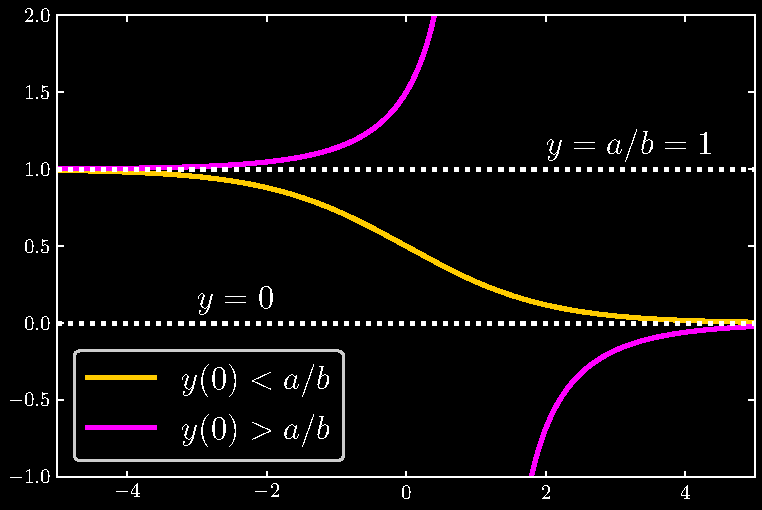
\includegraphics[width=1.0\textwidth]{../chap1/sec1.7/chap1sec1.7ex15.eps}
\end{center}

\newpage
% QUESTION 16
\qs{1.7.16}{(Cubic nonlinearity) The equation \(y' = y \!\left( 1 - y \right) \!\left( 2 - y \right) \) has \textbf{three steady states}: \(Y = 0, 1, 2\). By computing the derivative \(df /dy\) at \(y = 0, 1, 2\), decide whether each of these states is stable or unstable.

Draw the \textit{stability line} for this equation, to show \(y \!\left( t \right) \) leaving the unstable \(Y\)'s. Sketch a graph that shows \(y \!\left( t \right) \) starting from \(y \!\left( 0 \right) = \frac{1}{2}\) and \(\frac{3}{2}\) and \(\frac{5}{2}\).}

Given \(f \!\left( y \right) = y \!\left( 1 - y \right) \!\left( 2 - y \right) \), we have
\begin{align*}
	\frac{d f}{d y} & = \!\left( 1 - y \right) \!\left( 2 - y \right) + y \left[ - \!\left( 2 - y \right) - \!\left( 1 - y \right)  \right] \\
			& = \!\left( 2 - 3y + y^{2} \right) + y \!\left( - 3 + 2y \right) \\
			& = \!\left( 2 - 3y + y^{2} \right) - 3y + 2y^{2} \\
			& = 2 - 6y + 3y^{2}  
\end{align*}
At the values \(y = 0, 1, 2\), we have
\begin{align*}
	\frac{d f}{d y}_{\!\left( y = 0 \right)} & = 2 \\
	\frac{d f}{d y}_{\!\left( y = 1 \right) } & = -1 \\ 
	\frac{d f}{d y}_{\!\left( y = 2 \right) } & = 2
\end{align*}

Therefore, \(Y = 1\) is a stable state, while \(Y = 0, 2\) are unstable.

\begin{center}
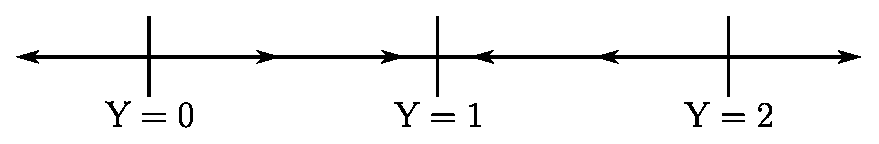
\includegraphics[width=1.0\textwidth]{../chap1/sec1.7/c1s7q16.eps}
\end{center}

Using the stability line, we can capture the trajectories that beginning at different initial conditions takes us on. Starting from \(y \!\left( 0 \right) = 1/2 \), we can observe that \(y \!\left( t \right) \) approaches \(Y = 1\). So too when we begin at \(y \!\left( 0 \right) = 3/2\). However, when we commence at \(y \!\left( 0 \right) = 5/2\), \(y \!\left( t \right) \) diverges to \(+\infty\).

The equation really needs to be solved numerically. You can start to attempt an analytic approach by separable variables, and writing
\[
	\int^{y \!\left( t \right) }_{y \!\left( 0 \right) } \frac{dY}{Y \!\left( 1 - Y \right) \!\left( 2 - Y  \right) } = \int^{t}_{0}  \, dT
\]

Using partial fractions decomposition, the left-hand side is equal to
\[
	\int^{y \!\left( t \right) }_{y \!\left( 0 \right) } \!\left(  \frac{1}{2Y} + \frac{1}{1 - Y} - \frac{1}{2 \!\left( 2 - Y \right) }\right) \, dY 
\]
Multiply the integrand through by \(2\) (you'll see why in a moment). Enabling us to solve as follows:
\begin{align*}
	\left[ \ln\left( Y \right) - \ln\left( 1 - Y \right)^{2} - \ln\left( \!\left( 2 - Y \right) \right) \right]  \Biggr|^{y \!\left( t \right)}_{y \!\left( 0 \right) } & = \ln\left( \frac{y \!\left( t \right)}{\!\left( 1 - y \!\left( t \right)  \right)^{2} \!\left( 2 - y \!\left( t \right)  \right)} \right) \\ 
 	  & \ - \ln\left( \frac{y \!\left( 0 \right)}{\!\left( 1 - y \!\left( 0 \right)  \right)^{2} \!\left( 2 - y \!\left( 0 \right)  \right) } \right) \\ 
\end{align*}

Let the second term equal a constant \(-c\). On the right-hand side, we have
\[
	\int^{t}_{0} 2 \, dT = 2t 
\]
Equating both sides and exponentiating, we have
\[
	\frac{y \!\left( t \right) }{\!\left( 1 - y \!\left( t \right)  \right)^{2} \!\left( 2 - y \!\left( t \right)  \right) } = Ce^{2t}
\]
where \(C = e^{c}\). Let me know if you find a way to analytically proceed! 

\vspace{12pt}

% QUESTION 17
\qs{1.7.17}{\begin{enumerate}[label=(\alph*)]
	\item Find the steady states of the \textbf{Gompertz equation} \(dy / dt = y \!\left( 1 - \ln\left( y \right) \right) \).
	\item Show that \(z = \ln\left( y \right)\) satisfies the linear equation \(dz / dt = 1 - z\).
	\item The solution \(z \!\left( t \right) = 1 + e^{-t} \!\left( z \!\left( 0 \right) - 1 \right) \) gives what formula for \(y \!\left( t \right) \) from \(y \!\left( 0 \right) \)?
\end{enumerate}}

\textbf{(a)} The unambiguous steady state is \(Y = e\). Technically, the Gompertz equation \(f \!\left( y \right) = y \!\left( 1 - \ln\left( y \right) \right) \) is not defined at \(Y = 0\). It seems that the author considers \(Y = 0\) as a second steady state, however.

\vspace{12pt}

\textbf{(b)} From the definition of \(z\), we have
\[
	\frac{d z}{d t} = \frac{1}{y} \frac{d y}{d t} 
\]
By (a), we then derive
\[
	\frac{d z}{d t} = \frac{1}{y} \left[ y \!\left( 1 - \ln\left( y \right) \right)  \right] = 1 - \ln\left( y \right) = 1 - z 
\]

\vspace{12pt}

\textbf{(c)} We can rewrite this solution as
\[
	\ln\left( y \!\left( t \right)  \right) = 1 + e^{-t} \!\left( \ln\left( y \!\left( 0 \right) \right) - 1 \right) 
\]
Exponentiating yields
\[
	y \!\left( t \right) = \exp\left( 1 + e^{-t} \!\left( \ln\left( y \!\left( 0 \right)  \right) - 1 \right)  \right)
\]

Now, observe that	
\[
	\frac{d f}{d y} = - \ln\left( y \right)
\]
When \(Y = 0 + \epsilon \), for real, positive, and arbitrarily small \(\epsilon \), we have \(df / dy > 0\), so we have an unstable steady state. By contrast, when \(Y = e\), \(df / dy < 0\), a stable steady state. 

Suppose now that we have three cases: \(0 < y \!\left( 0 \right) < e\), \(y \!\left( 0 \right) = e\), and \(y \!\left( 0 \right) > e\). Our solution curves now look like

\begin{center}
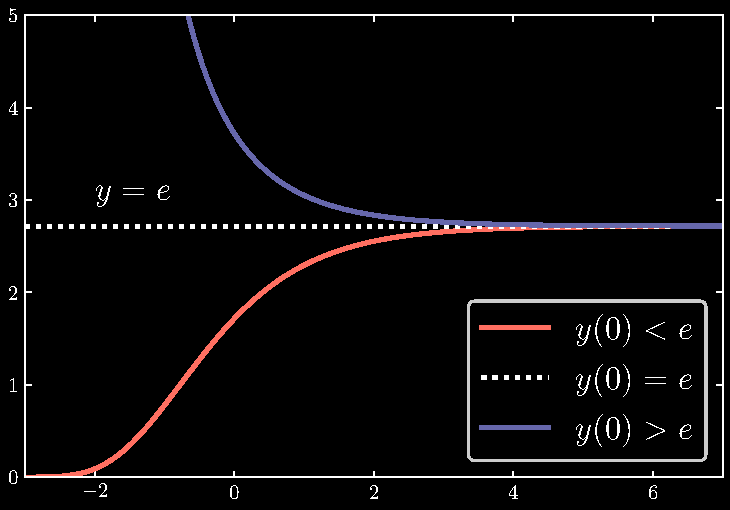
\includegraphics[width=1.0\textwidth]{../chap1/sec1.7/chap1sec1.7ex17.eps}
\end{center}

% QUESTION 18
\qs{1.7.18}{Decide stability or instability for the steady states of

\begin{enumerate}[label=(\alph*)]
	\item \(dy/dt = 2 \!\left( 1 - y \right) \!\left( 1 - e^{y} \right) \)
	\item \(dy/dt = \!\left( 1 - y^{2} \right) \!\left( 4 - y^{2} \right) \)
\end{enumerate}}

\textbf{(a)} When \(Y = 0\) or \(Y = 1\), \(f \!\left( y \right) = 0\). Then differentiating gives us
\[
	\frac{d f}{d y} = - 2 \left[\!\left( 1 - y \right) e^{y} + \!\left( 1 - e^{y} \right)  \right]
\]
with
\begin{alignat*}{3}
	\frac{d f}{d y}_{\!\left( Y = 0 \right) } & = -2 < 0 & \text{(unstable)} \\
	\frac{d f}{d y}_{\!\left( Y = 1 \right) } & = -2 \!\left( 1 - e \right) > 0 & \text{(stable)} \\ 
\end{alignat*}

\textbf{(b)} When \(Y = \pm 1\) or \(Y = \pm 2\), \(f \!\left( y \right) = 0\). Then differentiating gives us
\[
	\frac{d f}{d y} = -2y \!\left( 5 - 2y^{2} \right)
\]
with
\begin{alignat*}{3}
	&\frac{d f}{d y}_{\!\left( Y = -1 \right) } && = 6 > 0 & \text{(unstable)}  \\
	&\frac{d f}{d y}_{\!\left( Y = 1 \right) } && = - 6 < 0 & \text{(stable)} \\ 
	&\frac{d f}{d y}_{\!\left( Y = -2 \right) } && = -12 < 0 & \text{(stable)} \\
	&\frac{d f}{d y}_{\!\left( Y = 2 \right) } && = 12 > 0 & \text{(unstable)}
\end{alignat*}

% QUESTION 19
\qs{1.7.19}{Stefan's Law of Radiation is \(dy/dt = K \!\left( M^{4} - y^{4} \right) \). It is unusual to see fourth powers. Find all real steady states and their stability. Starting from \(y \!\left( 0 \right) = M/2\), sketch a graph of \(y \!\left( t \right) \).}

We have \(f \!\left( y \right) = 0\) when \(y = \pm M, \pm iM\). We will only consider the real roots. The derivative of \(f \!\left( y \right) \) is
\[
	\frac{d f}{d y} = -4Ky^{3}
\]
which corresponds to
\begin{alignat*}{3}
	&\frac{d f}{d y}_{\!\left( Y = M \right) } && = -4KM^{3} < 0 & \text{(stable)} \\
	&\frac{d f}{d y}_{\!\left( Y = -M \right) } && = 4KM^{3} > 0 & \text{(unstable)} \\ 
\end{alignat*}

Beginning from \(y \!\left( 0 \right) = M/2\), \(y \!\left( t \right) \) approaches the stable steady state at \(Y = M\).

\vspace{12pt}

% QUESTION 20
\qs{1.7.20}{\(dy/dt = ay - y^{3}\) has how many steady states \(Y\) for \(a < 0\) and then \(a > 0\)? Graph those values \(Y \!\left( a \right) \) to see a \textit{pitchfork bifurcation}--new steady states suddenly appear as \(a\) passes zero. The graph of \(Y \!\left( a \right) \) looks like a pitchfork.}

\(\bm{a > 0}\): In the case where \(a\) is positive, we certainly have \(Y = 0\) as one steady state. Then we must also have \(Y = \pm \sqrt{a}\) as two other steady states. 

To derive the stability, calculate
\[
	\frac{d f}{d y} = a - 3y^{2}
\]
which corresponds to
\begin{alignat*}{3}
	&\frac{d f}{d y}_{\!\left( Y = -\sqrt{a} \right) } && = -2a < 0 & \text{(stable)} \\
	&\frac{d f}{d y}_{\!\left( Y = 0 \right) } && = a > 0 & \text{(unstable)} \\
	&\frac{d f}{d y}_{\!\left( Y = \sqrt{a} \right) } && = -2a < 0 & \text{(stable)}
\end{alignat*}

\(\bm{a < 0}\): When \(a\) is negative, we only have \(Y = 0\) as the steady state (as far as real roots go, and we stay in the realm of the reals for now).

Since \(a < 0\), \(df/dy = a < 0\) implies that the steady state is stable.

\begin{center}
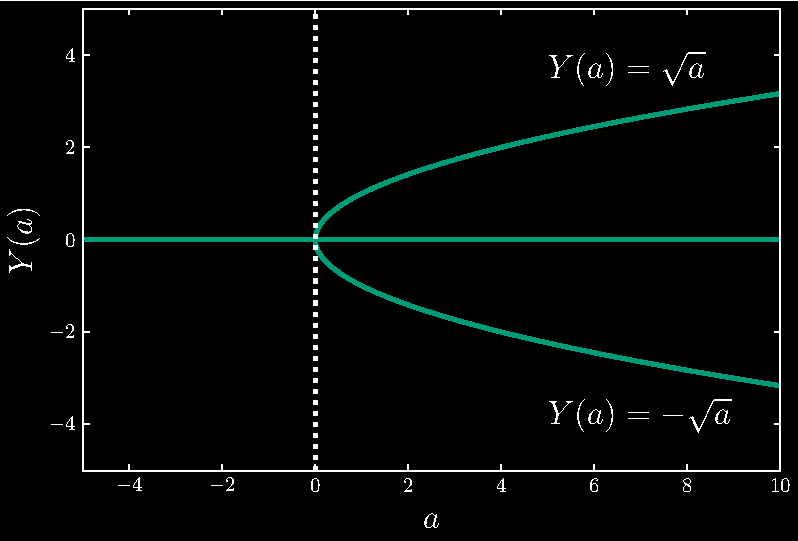
\includegraphics[width=1.0\textwidth]{../chap1/sec1.7/chap1sec1.7ex20.eps}
\end{center}

% QUESTION 21
\qs{1.7.21}{(Recommended) The equation \(dy/dt = \sin y\) has \textbf{infinitely many steady states.} What are they and which ones are stable? Draw the stability line to show whether \(y \!\left( t \right) \) increases or decreases when \(y \!\left( 0 \right) \) is between two of the steady states.}

When \(f \!\left( y \right) = \sin y = 0\), we have \(Y = N \pi\) for all integer \(N\). Since \(df/dy = \cos y\), we have the cases:
\[
	Y \text{ is: }\begin{cases}
		\text{stable,} & N = 2k + 1, k \in \mathbb{Z}  \\
		\text{unstable,} & N = 2k, k \in \mathbb{Z} \\
	\end{cases}
\]

The stability line is pictured below:

\begin{center}
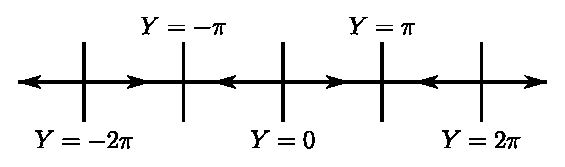
\includegraphics[width=1.0\textwidth]{../chap1/sec1.7/c1s7q21.eps}
\end{center}

% QUESTION 22
\qs{1.7.22}{Change Problem 21 to \(dy/dt = \!\left( \sin y \right)^{2}\). The steady states are the same, but now the derivative of \(f \!\left( y \right) = \!\left( \sin y \right)^{2}\) is zero at all those states (because \(\sin y\) is zero). What will the solution actually do if \(y \!\left( 0 \right) \) is between two steady states?}

Here, we have
\[
	\frac{d f}{d y} = 2 \sin y \cos y = \sin 2y
\]
where for \(Y\) such that \(f \!\left( Y \right) = 0\), we also have \(df/dy = 0\). These \(Y\)'s are of the form
\[
	Y = n \pi 
\]

for all integers \(n\).

At the moment, it is ambiguous as to what type of stability each steady state is in. In fact, we call this \textbf{marginal stability}. To further investigate, we must go to the \textbf{second derivative} of \(f \!\left( y \right) \). To motivate this, let \(Y\) be our steady state, and let \(\epsilon \!\left( t \right) \) be some small perturbation around the steady state. Our \(y \!\left( t \right) \) is given by
\[
	y \!\left( t \right) = Y + \epsilon \!\left( t \right) 
\]
Differentiating both sides, taking into account that \(Y\) is a constant, we derive
\[
	y' \!\left( t \right) = \epsilon' \!\left( t \right) 
\]
And since \(y' \!\left( t \right) = f \!\left( y \right) \), we have
\[
	\epsilon' \!\left( t \right) = f \!\left( Y + \epsilon \!\left( t \right)  \right) 
\]
Using the Taylor series expansion, we may write
\[
	\epsilon' \!\left( t \right) = f \!\left( Y \right) + \epsilon f' \!\left( Y \right) + \epsilon^{2} f'' \!\left( Y \right) / 2 + \cdots 
\]
Note that the first two terms on the right side vanish, since \(f \!\left( Y \right) = f' \!\left( Y \right) = 0\). We should also ignore higher-order terms. That leaves us with the approximation
\[
	\epsilon' \!\left( t \right) \approx \epsilon^{2} f'' \!\left( Y \right) /2
\]
Now in this case, observe that
\[
	f'' \!\left( y \right) = 2 \left( \cos^{2}y - \sin^{2}y \right) = 2 \cos 2y
\]

We can conclude that for any of our aforementioned steady states \(Y\), which are of form \(n \pi \) for integers \(n\), it \textit{must} be the case that
\[
	f''\!\left( Y \right) > 0
\]
Moreover, since \(\epsilon^{2}\) is always positive irrespective of the value of \(\epsilon \!\left( t \right) \), we can now conclude that
\[
	\epsilon' \!\left( t \right) > 0
\]
Therefore, going back to the equality between \(y'\!\left( t \right) \) and \(\epsilon' \!\left( t \right) \), it immediately follows that
\[
	y'\!\left( t \right) > 0
\]
So for any perturbation \(\epsilon \!\left( t \right) \), we will have increasing \(y \!\left( t \right) \), meaning that \(y \!\left( t \right) \) will indefinitely move to successively higher steady states \(Y\).\footnote{\href{https://math.libretexts.org/Bookshelves/Differential_Equations/Differential_Equations_(Chasnov)/08\%3A_Nonlinear_Differential_Equations/8.01\%3A_Fixed_Points_and_Stability}{See this LibreText chapter on fixed points and stability here.}}

\vspace{12pt}

% QUESTION 23
\qs{1.7.23}{(\textit{Research project}) Find actual data on the US population in the years 1950, 1980, and 2010. What values of \(a\), \(b\), \(d\) in the solution formula (7) will fit these values? is the formula accurate at 2000, and what population does it predict for 2020 and 2100?

You could reset \(t = 0\) to the year 1950 and rescale time so that \(t = 3\) is 1980.}

Will return to this with some numerical methods.

\vspace{12pt}

% QUESTION 24
\qs{1.7.24}{If \(dy/dt = f \!\left( y \right) \), what is the limit \(y \!\left( \infty \right) \) starting from each point \(y \!\left( 0 \right) \)?

\begin{center}
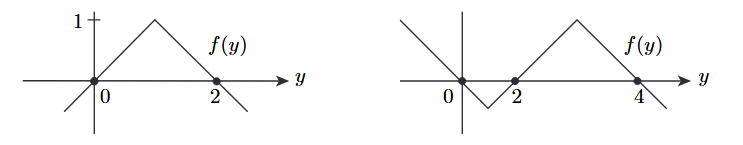
\includegraphics[width=1.0\textwidth]{../chap1/sec1.7/c1s7q24.png}
\end{center}}

In the first graph, we have \(f \!\left( y \right) = 0\) when \(Y = 0\), \(2\). At these respective points, \(f'\!\left( y \right) > 0\) and \(f'\!\left( y \right) < 0\). Then \(Y = 0\) is an unstable steady state, while \(Y = 2\) is stable. As such, we have the cases
\[
	y \!\left( \infty \right) = \begin{cases}
		- \infty & y \!\left( 0 \right) < 0 \\
		2 & y \!\left( 0 \right) > 0  \\
	\end{cases}
\]
For the second graph, we have steady states at \(Y = 0\), \(2\), and \(4\). At each of those points, we have \(f'\!\left( y \right) < 0\), \(f'\!\left( y \right) > 0\), and \(f' \!\left( y \right) < 0\), respectively. These steady states are, in order, stable, unstable, and stable. We have the cases
\[
	y \!\left( \infty \right) = \begin{cases}
		0 & y \!\left( 0 \right) < 2 \\
		4 & y \!\left( 0 \right) > 2 \\
	\end{cases}
\]

% QUESTION 25
\qs{1.7.25}{
\begin{enumerate}[label=(\alph*)]
	\item Draw a function \(f \!\left( y \right) \) so that \(y \!\left( t \right) \) approaches \(y \!\left( \infty \right) = 3\) from every \(y \!\left( 0 \right) \).
	\item Draw \(f \!\left( y \right) \) so that \(y \!\left( \infty \right) = 4\) if \(y \!\left( 0 \right) > 0\) and \(y \!\left( \infty \right) = -2\) if \(y \!\left( 0 \right) < 0\).
\end{enumerate}}

\textbf{(a)} Consider the function
\[
	f \!\left( y \right) = 3 - y
\]
Then \(f \!\left( Y \right) = 0\) when \(Y = 3\), and \(df/dy = -1\) for all \(y\). Thus \(Y = 3\) is a stable steady state.

\begin{center}
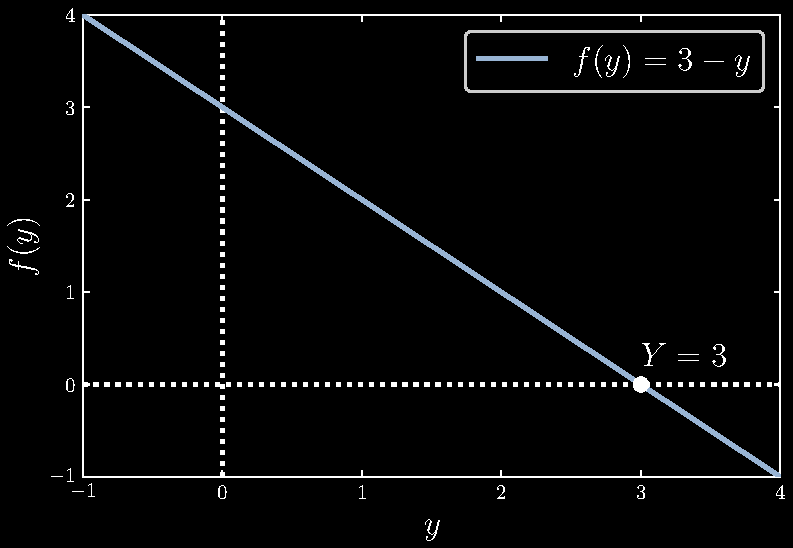
\includegraphics[width=1.0\textwidth]{../chap1/sec1.7/chap1sec1.7ex25a.eps}
\end{center}

\textbf{(b)} Here, we must have \(Y = 4\) and \(Y = -2\) as stable steady states, and \(Y = 0\) as an unstable steady state. One approach is to define a piecewise function as follows:
\[
	f \!\left( y \right) = \begin{cases}
		-2 - y & y \le -1 \\
		y & -1 < y \le 2 \\
		4 - y & 2 < y \\
	\end{cases}
\]
\begin{center}
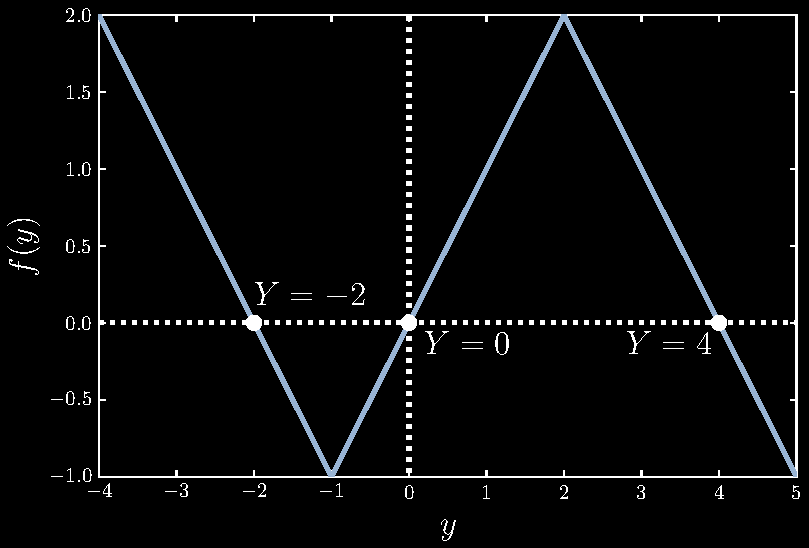
\includegraphics[width=1.0\textwidth]{../chap1/sec1.7/chap1sec1.7ex25b.eps}
\end{center}

which is consistent with the stability of each of the steady states:
\begin{alignat*}{4}
	&\frac{d f}{d y}_{\!\left( Y = -2 \right) } && = & -1 \\
	&\frac{d f}{d y}_{\!\left( Y = 0 \right) } && = & 1 \\ 
	&\frac{d f}{d y}_{\!\left( Y = 4 \right) } && = & -1
\end{alignat*}

% QUESTION 26
\qs{1.7.26}{Which exponents \(n\) in \(dy/dt = y^{n}\) produce blowup \(y \!\left( T \right) = \infty\) in a finite time? You could separate the equation into \(dy/y^{n} = dt\) and integrate from \(y \!\left( 0 \right) = 1\).}

First consider the case that \(n = 1\). Then we have
\begin{alignat*}{3}
	\implies && \int^{y \!\left( t \right) }_{y \!\left( 0 \right) } \frac{dy}{y} & = \int^{t}_{0} \, dT \\
	\implies && \ln\left( y \!\left( t \right)  \right) - \ln\left( y \!\left( 0 \right)  \right) & = t \\ 
	\implies&& y \!\left( t \right) & = e^{t}
\end{alignat*}
which does \textbf{not} blowup to \(\infty\) in a finite time. In the general case, however, we have
\begin{alignat*}{3}
	\implies &&\int^{y \!\left( t \right) }_{y \!\left( 0 \right) } \frac{dy}{y^{n}} & = \int^{t}_{0}  \, dT  \\
	\implies &&-\frac{1}{n-1} \!\left( y^{-\!\left( n - 1 \right) } - 1 \right) & = t \\ 
	\implies&& y^{n-1} \!\left( t \right) & = \frac{1}{1 - \!\left( n - 1 \right) t} 
\end{alignat*}

where it is apparent that \(y \!\left( t \right) \) diverges to infinity at finite time for
\[
	T = \frac{1}{n - 1}
\]
We may conclude that for \(n > 1\), there exists a finite time \(T\) where \(y \!\left( t \right) \) diverges to infinity.

\vspace{12pt}

% QUESTION 27
\qs{1.7.27}{Find the steady states of \(dy/dt = y^{2} - y^{4}\) and decide whether they are stable, unstable, or one-sided stable. Draw a stability line to show the final value \(y \!\left( \infty \right) \) from each initial value \(y \!\left( 0 \right) \).}

Given \(f \!\left( y \right) = y^{2} - y^{4}\), we have \(Y = \pm 1\) and \(Y = 0\) corresponding to \(f \!\left( Y \right) = 0\).
\[
	f'\!\left( y \right) = 2y - 4y^{3}
\]
For \(Y = 1\), we have \(f'\!\left( Y = 1 \right) = -2 < 0\), a stable steady state. Conversely, for \(Y = -1\), we have \(f' \!\left( Y = -1 \right) = 2 > 0\), an unstable steady state.

The remaining steady state at \(Y = 0\) is somewhat problematic. Following the logic of question 1.7.22, we take the second derivative of \(f \!\left( y \right) \) to get
\[
	f''\!\left( y \right) = 2 - 12y^{2}
\]
which, for \(f''\!\left( Y = 0 \right) = 2 > 0\), implies that for any perturbation \(\epsilon \!\left( t \right) \), we have \(\epsilon' \!\left( t \right) > 0\), implying that \(y'\!\left( t \right) > 0\), and thus increasing \(y \!\left( t \right) \). Finally, we can conclude that the stability line looks like:

\begin{center}
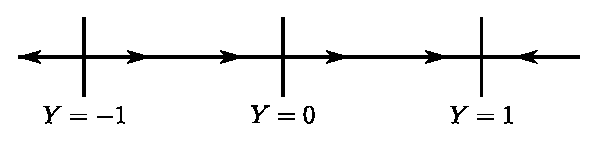
\includegraphics[width=1.0\textwidth]{../chap1/sec1.7/c1s7q27.eps}
\end{center}

% QUESTION 28
\qs{1.7.28}{For an autonomous equation \(y' = f \!\left( y \right) \), why is it impossible for \(y \!\left( t \right) \) to be increasing at one time \(t_{1}\) and decreasing at another time \(t_{2}\)?}

The crux of the explanation has to do with \textbf{steady states}. First consider the case where either \(y \!\left( 0 \right) \) lies above or below a stable steady state. We can think of a stable steady state as a kind of ``attractor''; a magnet or celestial body that pulls a point particle onto it. 

In this case, the point particle moves \textbf{monotonically} in \textbf{one} direction towards the stable steady state, so we cannot have \(y'\!\left( t_{1} \right) > 0\) and \(y'\!\left( t_{2} \right) < 0\), \(t_{1} \neq t_{2}\), simultaneously.

In the case where there is no stable steady state (such as in the overharvesting case), \(y \!\left( t \right) \) diverges to \(-\infty\) -- once again, monotonically. 

\newpage
\subsection{\textsf{1.8 - Separable Equations and Exact Equations}}
% QUESTION 1
\qs{1.8.1}{Finally we can solve the example \(dy/dt = y^{2}\) in Section 1.1 of this book.

Start from \(y \!\left( 0 \right) = 1\). Then \(\displaystyle{\int^{y}_{1} \frac{dy}{y^{2}} = \int^{t}_{0}  \, dt  }\). Notice the limits on \(y\) and \(t\). Find \(y \!\left( t \right) \).}

Solve as follows:

\begin{alignat*}{3}
	\implies &&\int^{y}_{1} \frac{dy}{y^{2}} & = \int^{t}_{0}  \, dt  \\
	\implies && -y^{-1} + 1 & = t \\ 
	\implies && y \!\left( t \right) & = \frac{1}{1 - t}
\end{alignat*}

% QUESTION 2
\qs{1.8.2}{Start the same equation \(dy/dt = y^{2}\) from any value \(y \!\left( 0 \right) \). At what time \(t\) does the solution blow up? For which starting values \(y \!\left( 0 \right) \) does it never blow up?}

Let \(y \!\left( 0 \right) = a\). Then we have
\[
	y \!\left( t \right) = \frac{1}{a^{-1} - t} = \frac{a}{1 - at}
\]

In general, \(y \!\left( t \right) \) blows up at \(t = 1/a\). Suppose that \(a \le 0\). Then the denominator \(1 - at\) never approaches zero, so \(y \!\left( t \right) \) never diverges to infinity.

\vspace{12pt}

% QUESTION 3
\qs{1.8.3}{Solve \(dy/dt = a \!\left( t \right) y\) as a separable equation starting from \(y \!\left( 0 \right) = 1\), by choosing \(f \!\left( y \right) = 1/y\). This equation gave the growth factor \(G \!\left( 0,t \right) \) in Section 1.6.}

Solve as follows:

\begin{alignat*}{3}
	\implies &&\int^{y \!\left( t \right) }_{1} \frac{dy}{y} & = \int^{t}_{0} a \!\left( t \right)  \, dt  \\
	\implies && \ln\left( y \!\left( t \right)  \right) & = \int^{t}_{0} a \!\left( t \right)  \, dt  \\ 
	\implies && y \!\left( t \right) & = e^{\int^{t}_{0} a \!\left( t \right)  \, dt }
\end{alignat*}

% QUESTION 4
\qs{1.8.4}{Solve these separable equations starting from \(y \!\left( 0 \right) = 0\):

\begin{enumerate}[label=(\alph*)]
	\item \(\displaystyle{\frac{d y}{d t} = ty}\)
	\item \(\displaystyle{\frac{d y}{d t} = t^{m}y^{n}}\)
\end{enumerate}}

Ignore the initial condition. We cannot have it at zero.

\textbf{(a)}
\begin{alignat*}{3}
	\implies &&\int^{y \!\left( t \right) }_{0} \frac{dy}{y} & = \int^{t}_{0} t \, dt  \\
	\implies && \ln\left( y \!\left( t \right)  \right) - \ln\left( y \!\left( 0 \right)  \right) & = \frac{t^{2}}{2} \\
	\implies && y \!\left( t \right) & = y \!\left( 0 \right) e^{t^{2}/2}
\end{alignat*}

\textbf{(b)} 
\begin{alignat*}{3}
	\implies &&\int^{y \!\left( t \right) }_{y \!\left( 0 \right) } \frac{dy}{y^{n}} & = \int^{t}_{0} t^{m} \, dt  \\
	\implies && -\frac{1}{n-1} \!\left(  y \!\left( t \right)^{-\!\left( n - 1 \right) } - y \!\left( 0 \right)^{-\!\left( n - 1 \right) }\right) & = \frac{1}{m + 1}t^{m + 1} \\ 
	\implies && y \!\left( t \right)^{-\!\left( n - 1 \right) } & = y \!\left( 0 \right)^{-\!\left( n - 1 \right) } - \frac{n - 1}{m + 1}t^{m + 1} \\
	\implies && y \!\left( t \right) & = \left[ y \!\left( 0 \right)^{-\!\left( n - 1 \right) } - \frac{n - 1}{m + 1}t^{m + 1} \right]^{\frac{1}{1 - n}} 
\end{alignat*}

% QUESTION 5
\qs{1.8.5}{Solve \(\displaystyle{\frac{d y}{d t} = a \!\left( t \right) y^{2} = \frac{a \!\left( t \right) }{1/y^{2}}}\) as a separable equation starting from \(y \!\left( 0 \right) = 1\).}

Solve as follows:

\begin{alignat*}{3}
	\implies && \int^{y \!\left( t \right) }_{y \!\left( 0 \right) } \frac{dy}{y^{2}} & = \int^{t}_{0} a \!\left( t \right)  \, dt  \\
	\implies && -\!\left( y \!\left( t \right)^{-1} - y \!\left( 0 \right)^{-1} \right) & = \int^{t}_{0} a \!\left( t \right)  \, dt  \\ 
	\implies && y \!\left( t \right)  & = \left[ y \!\left( 0 \right)^{-1} - \int^{t}_{0} a \!\left( t \right)  \, dt  \right]^{-1} \\
		 && & = \left[ 1 - \int^{t}_{0} a \!\left( t \right)  \, dt  \right]^{-1}
\end{alignat*}

% QUESTION 6
\qs{1.8.6}{The equation \(\displaystyle{\frac{d y}{d t} = y + t}\) is not separable or exact. But it is linear and \(y = \) \underline{\qquad}.}

Use an integrating factor: \(e^{-t}\).

\begin{alignat*}{3}
	\implies && \!\left( e^{-t}y \right)' & = te^{-t} \\
	\implies && e^{-t} y \!\left( t \right) - y \!\left( 0 \right)  & = \int^{t}_{0} te^{-t} \, dt  \\ 
	\implies && y \!\left( t \right) & = e^{t} y \!\left( 0 \right) - \!\left( 1 + t - e^{t} \right) 
\end{alignat*}

% QUESTION 7
\qs{1.8.7}{The equation \(\displaystyle{\frac{d y}{d t} = \frac{y}{t}}\) has the solution \(y = At\) for every constant \(A\). Find this solution by separating \(f = 1/y\) from \(g = 1/t\). Then integrate \(dy/y = dt/t\). Where does the constant \(A\) come from?}

Solve as follows:

\begin{alignat*}{3}
	\implies && \int^{y \!\left( t \right) }_{y \!\left( 0 \right) } \frac{dy}{y} & = \int^{t}_{t_{0}} \frac{dt}{t}  \\
	\implies && \ln\left( y \!\left( t \right)  \right) - \ln\left( y \!\left( 0 \right)  \right) & = \ln\left( t \right) - \ln\left( t_{0} \right) \\
	\implies && y \!\left( t \right) & = \frac{y \!\left( 0 \right) }{t_{0}} t
\end{alignat*}

Lastly, define \(A = y \!\left( 0 \right) / t_{0}\).

\vspace{12pt}

% QUESTION 8
\qs{1.8.8}{For which number \(A\) is \(\displaystyle{\frac{d y}{d t} = \frac{ct - ay}{At + by}}\) an exact equation? For this \(A\), solve the equation by finding a suitable function \(F \!\left( y,t \right) + C \!\left( t \right) \).}

The exactness condition is met when
\[
	\frac{\partial g}{\partial y} = -\frac{\partial f}{\partial t} 
\]
Here, we are given
\[
	g \!\left( y, t \right) = ct - ay \quad \text{and} \quad f \!\left( y,t \right) = At + by
\]
Thus we must have
\[
	\frac{\partial g}{\partial y} = -a = -A = -\frac{\partial f}{\partial t} 
\]
Implying that \(A = a\). First, we find \(F \!\left( y,t \right) + C \!\left( t \right) \):
\[
	\int \!\left( at + by \right)  \, dy  = aty + \frac{by^{2}}{2} + C \!\left( t \right)
\]

Next, we differentiate with respect to \(t\) to find
\[
	\frac{\partial }{\partial t} \!\left( aty + \frac{by^{2}}{2} + C \!\left( t \right)  \right) = ay - ct
\]
Implying that
\[
	C \!\left( t \right) = -\frac{ct^{2}}{2}
\]
Thus the equation is solved by
\[
	F \!\left( y,t \right) + C \!\left( t \right) = aty + \frac{by^{2}}{2} - \frac{ct^{2}}{2} = \text{constant}
\]

% QUESTION 9
\qs{1.8.9}{Find a function \(y \!\left( t \right) \) different from \(y = t\) that has \(dy/dt = y^{2}/t^{2}\).}

Solve as follows:

\begin{alignat*}{3}
	\implies &&\int \frac{dy}{y^{2}} & = \int \frac{dt}{t^{2}} \\
	\implies && -y^{-1} & = -t^{-1} + C \\ 
	\implies && y \!\left( t \right) & = \frac{t}{1 + tC}
\end{alignat*}

The given example has \(C = 0\). Simply choose any nonzero \(C\). More concretely, the choice of \(C\) is given by

\begin{alignat*}{3}
	\implies &&\int^{y \!\left( t \right) }_{y \!\left( 0 \right) } \frac{dy}{y^{2}} & = \int^{t}_{t \!\left( 0 \right) } \frac{dt}{t^{2}}  \\
	\implies && -y \!\left( t \right)^{-1} + y \!\left( 0 \right)^{-1} & = -t^{-1} + t \!\left( 0 \right)^{-1} \\ 
	\implies && y \!\left( t \right) & = \left[ t^{-1} + y \!\left( 0 \right)^{-1} - t \!\left( 0 \right)^{-1} \right]^{-1} \\
		 && & = \frac{t}{1 + \!\left( y \!\left( 0 \right)^{-1} - t \!\left( 0 \right)^{-1} \right) t}
\end{alignat*}

where \(C\) is given by
\[
	C = y \!\left( 0 \right)^{-1} - t \!\left( 0 \right)^{-1}
\]

% QUESTION 10
\qs{1.8.10}{These equations are separable after factoring the right hand sides:
\[
	\text{Solve} \quad \frac{d y}{d t} = e^{y + t} \quad \text{and} \quad \frac{d y}{d t} = yt + y + t + 1
\]}

\textbf{(i)} Decompose the right hand side into \(e^{y}e^{t}\). Solve as follows:

\begin{alignat*}{3}
	\implies &&\int \frac{dy}{e^{y}} & = \int e^{t} \, dt \\
	\implies && -e^{-y} & = e^{t} + C \\ 
	\implies && y \!\left( t \right) & = -\ln\left( -e^{t} + C \right) 
\end{alignat*}

\textbf{(ii)} Factor the right hand side into \(\!\left( y + 1 \right) \!\left( t + 1 \right) \). Then solve as follows:

\begin{alignat*}{3}
	\implies &&\int \frac{dy}{y + 1} & = \int \!\left( t + 1 \right) \, dt \\
	\implies && \ln\left( y + 1 \right) & = \frac{t^{2}}{2} + t + C  \\ 
	\implies && y \!\left( t \right) & = \exp\left( \frac{t^{2}}{2} + t + C \right) - 1 
\end{alignat*}

% QUESTION 11
\qs{1.8.11}{These equations are linear and separable: Solve \(\displaystyle{\frac{d y}{d t} = \!\left( y + 4 \right) \cos t}\) and \(\displaystyle{\frac{d y}{d t} = ye^{t}}\).}

We write
\begin{alignat*}{3}
	\implies && \int^{y \!\left( t \right) }_{y \!\left( 0 \right) } \frac{dy}{y + 4} & = \int^{t}_{0} \cos\left( t \right) \, dt  \\
	\implies && \ln\left( \frac{y \!\left( t \right) + 4}{y \!\left( 0 \right) + 4} \right)& = \sin\left( t \right) \\ 
	\implies && y \!\left( t \right) & = \!\left( y \!\left( 0 \right) + 4 \right) e^{\sin\left( t \right)} - 4
\end{alignat*}

And for the second equation
\begin{alignat*}{3}
	\implies && \int^{y \!\left( t \right) }_{y \!\left( 0 \right) } \frac{dy}{y}  & = \int^{t}_{0} e^{t} \, dt  \\
	\implies && \ln\left( \frac{y \!\left( t \right) }{y \!\left( 0 \right) } \right) & = e^{t} - 1 \\
	\implies && y \!\left( t \right) & = y \!\left( 0 \right) e^{e^{t} - 1}
\end{alignat*}

% QUESTION 12
\qs{1.8.12}{Solve these three separable equations starting from \(y \!\left( 0 \right) = 1\):
\begin{enumerate}[label=(\alph*)]
	\item \(\frac{d y}{d t} = -4ty\)
	\item \(\frac{d y}{d t} = ty^{3}\)
	\item \(\!\left( 1 + t \right) \frac{d y}{d t} = 4y\)
\end{enumerate}}

Solve as follows:

(a) 

\begin{alignat*}{3}
	\implies && \int^{y \!\left( t \right) }_{y \!\left( 0 \right) } \frac{dy}{y}  & = -4 \int^{t}_{0} t \, dt  \\
	\implies && \ln\left( \frac{y \!\left( t \right) }{y \!\left( 0 \right) } \right) & = -4 \!\left( \frac{t^{2}}{2} \right)  \\ 
	\implies && y \!\left( t \right)  & = y \!\left( 0 \right) e^{-2t^{2}} \\
		 && & = e^{-2t^{2}}
\end{alignat*}

(b) 

\begin{alignat*}{3}
	\implies && \int^{y \!\left( t \right) }_{y \!\left( 0 \right) } \frac{dy}{y^{3}}  & = \int^{t}_{0} t \, dt  \\
	\implies && -\frac{1}{2} y \!\left( t \right)^{-2} + \frac{1}{2} y \!\left( 0 \right)^{-2} & = \frac{t^{2}}{2} \\ 
	\implies && y \!\left( t \right)^{-2} & = y \!\left( 0 \right)^{-2} - t^{2} \\
	\implies && y \!\left( t \right) & = \frac{y \!\left( 0 \right)}{\left[ 1 - \!\left( y \!\left( 0 \right)t \right)^{2} \right]^{1/2}} \\
		 && & = \frac{1}{\left[ 1 - \!\left( y \!\left( 0 \right) t \right)^{2} \right]^{1/2} }
\end{alignat*}

(c)

\begin{alignat*}{3}
	\implies && \int^{y \!\left( t \right) }_{y \!\left( 0 \right) } \frac{dy}{y}  & = 4 \int^{t}_{0} \!\left( 1 + t \right)  \, dt  \\
	\implies && \ln\left( \frac{y \!\left( t \right) }{y \!\left( 0 \right) } \right) & = 4\!\left( t + \frac{t^{2}}{2} \right)  \\ 
	\implies && y \!\left( t \right) & = y \!\left( 0 \right) e^{4t + 2t^{2}} \\
		 && & = e^{4t + 2t^{2}}
\end{alignat*}

\newpage

\textbf{Test the exactness condition \(\bm{\partial g / \partial y = -\partial f / \partial t}\) and solve Problems 13-14.}

\vspace{12pt}

% QUESTION 13
\qs{1.8.13}{
\begin{enumerate}[label=(\alph*)]
	\item \(\displaystyle{\frac{d y}{d t} = \frac{-3t^{2} - 2y^{2}}{4ty + 6y^{2}}}\)
	\item \(\displaystyle{\frac{d y}{d t} = -\frac{1 + ye^{ty}}{2y + te^{ty}}}\)
\end{enumerate}}

(a) The exactness condition is
\[
	\frac{\partial g}{\partial y} = -4y = -\frac{\partial f}{\partial t}  
\]

Next, we integrate \(f \!\left( y,t \right) \) with respect to \(y\):
\[
	\int \!\left( 4ty + 6y^{2} \right) \, dy = 2ty^{2} + 2y^{3} + C \!\left( t \right) 
\]
and differentiate \(F \!\left( y, t \right) + C \!\left( t \right) \) with respect to \(t\):
\[
	\frac{\partial }{\partial t} \!\left( F \!\left( y,t \right) + C \!\left( t \right)  \right) = 2y^{2} + C' \!\left( t \right) 
\]
which itself is equal to \(-g \!\left( y, t \right) \), implying that
\[
	C' \!\left( t \right) = 3t^{2} \quad \implies \quad C \!\left( t \right) = t^{3}
\]
Therefore, \(dy/dt\) is solved by
\[
	F \!\left( y,t \right) + C \!\left( t \right) = 2ty^{2} + 2y^{3} + t^{3}
\]

(b) The exactness condition is
\[
	\frac{\partial g}{\partial y} = -e^{ty} - tye^{ty} = -\frac{\partial f}{\partial t} 
\]
Next, we integrate \(f \!\left( y,t \right) \) with respect to \(y\):
\[
	\int \!\left( 2y + te^{ty} \right) \, dy = y^{2} + e^{ty} + C \!\left( t \right) 
\]
and differentiate \(F \!\left( y,t \right) + C \!\left( t \right) \) with respect to \(t\):
\[
	\frac{\partial }{\partial t} \!\left( F \!\left( y, t \right) + C \!\left( t \right)  \right) = ye^{ty} + C'\!\left( t \right)  
\]
which itself is equal to \(-g \!\left( y,t \right) \), implying that
\[
	C'\!\left( t \right) = 1 \quad \implies \quad C \!\left( t \right) = t
\]
Therefore, \(dy/dt\) is solved by
\[
	F \!\left( y,t \right) + C \!\left( t \right) = y^{2} + e^{ty} + t
\]

% QUESTION 14
\qs{1.8.14}{
\begin{enumerate}[label=(\alph*)]
	\item \(\displaystyle{\frac{d y}{d t} = \frac{4t - y}{t - 6y}}\)
	\item \(\displaystyle{\frac{d y}{d t} = - \frac{3t^{2} + 2y^{2}}{4ty + 6y^{2}}}\)
\end{enumerate}}

(a) The exactness condition is
\[
	\frac{\partial g}{\partial y} = -1 = \frac{\partial f}{\partial t} 
\]
Next, we integrate \(f \!\left( y,t \right) \) with respect to \(y\):
\[
	\int \!\left( t - 6y \right) \, dy = ty - 3y^{2} + C \!\left( t \right) 
\]
and differentiate \(F \!\left( y,t \right) + C \!\left( t \right) \) with respect to \(t\):
\[
	\frac{\partial }{\partial t} \!\left( F \!\left( y,t \right) + C \!\left( t \right)  \right) = y + C'\!\left( t \right) 
\]
which itself is equal to \(-g \!\left( y,t \right) \), implying that
\[
	C'\!\left( t \right) = -4t \quad \implies \quad C \!\left( t \right) = -2t^{2}
\]
Therefore, \(dy/dt\) is solved by
\[
	F \!\left( y,t \right) + C \!\left( t \right) = ty - 3y^{2} - 2t^{2}
\]
(b) The exactness condition is
\[
	\frac{\partial g}{\partial y} = -4y = -\frac{\partial f}{\partial t} 
\]
Next, we integrate \(f \!\left( y,t \right) \) with respect to \(y\):
\[
	\int \!\left( 4ty + 6y^{2} \right) \, dy = 2ty^{2} + 2y^{3} + C \!\left( t \right) 
\]
and differentiate \(F \!\left( y,t \right) + C \!\left( t \right) \) with respect to \(t\):
\[
	\frac{\partial }{\partial t} \!\left( F \!\left( y,t \right) + C \!\left( t \right)  \right) = 2y^{2} + C'\!\left( t \right)  
\]
which itself is equal to \(-g \!\left( y,t \right) \), implying that
\[
	C'\!\left( t \right) = 3t^{2} \quad \implies \quad C \!\left( t \right) = t^{3}
\]
Therefore, \(dy/dt\) is solved by
\[
	F \!\left( y,t \right) + C \!\left( t \right) = 2ty^{2} + 2y^{3} + t^{3}
\]
% QUESTION 15
\qs{1.8.15}{Show that \(\displaystyle{\frac{d y}{d t} = -\frac{y^{2}}{2ty}}\) is exact but the same equation \(\displaystyle{\frac{d y}{d t} = -\frac{y}{2t}}\) is not exact. Solve both equations. (This problem suggests that many equations become exact when multiplied by an integrating factor.)}

In the first case, we have \(g \!\left( y,t \right) = -y^{2}\) and \(f \!\left( y,t \right) = 2ty\). Then
\[
	\frac{\partial g}{\partial y} = -2y = -\frac{\partial f}{\partial t} 
\]
In the second case, \(g \!\left( y,t \right) = -y\) and \(f \!\left( y,t \right) = 2t\), establishing
\[
	\frac{\partial g}{\partial y} = -1 \neq -2 = -\frac{\partial f}{\partial t} 
\]
We solve the first equation as follows: first integrate \(f \!\left( y,t \right) \) with respect to \(y\):
\[
	\int 2ty \, dy = ty^{2}	+ C \!\left( t \right) 
\]
and then differentiate with respect to \(t\):
\[
	\frac{\partial }{\partial t} \!\left( F \!\left( y,t \right) + C \!\left( t \right)  \right) = y^{2} + C'\!\left( t \right) 
\]
which itself is equal to \(-g \!\left( y,t \right) \), allowing us to deduce
\[
	C'\!\left( t \right) = 0 \quad \implies C \!\left( t \right) = c
\]
where \(c\) is a constant. Then the equation is solved by
\[
	F \!\left( y,t \right) + C \!\left( t \right) = ty^{2} + c
\]
The second equation is separable, so we write
\begin{alignat*}{3}
	\implies && \int^{y \!\left( t \right) }_{y \!\left( 0 \right) } \frac{dy}{y}  & = -\int^{t}_{t \!\left( 0 \right) } \frac{dt}{2t}  \\
	\implies && \ln\left( \frac{y \!\left( t \right) }{y \!\left( 0 \right) } \right) & = -\frac{1}{2} \ln\left( \frac{t}{t \!\left( 0 \right) } \right) \\
	\implies && y \!\left( t \right) & = y \!\left( 0 \right) \!\left( \frac{t}{t \!\left( 0 \right) } \right)^{-1/2}
\end{alignat*}

\newpage

% QUESTION 16
\qs{1.8.16}{Exactness is really the condition to solve two equations with the same function \(H \!\left( t,y \right) \):
\[
	\frac{\partial H}{\partial y} = f \!\left( t,y \right) \quad \text{and} \quad \frac{\partial H}{\partial t} = - g \!\left( t,y \right) \quad \text{can be solved if} \quad \frac{\partial f}{\partial t} = - \frac{\partial g}{\partial y}  
\]
Take the \(t\) derivative of \(\partial H / \partial y\) and the \(y\) derivative of \(\partial H / \partial t\) to show that exactness is \textit{necessary}. It is also \textit{sufficient} to guarantee that a solution \(H\) will exist.}

We have
\[
	\frac{d }{d t} \frac{\partial H}{\partial y} = \frac{\partial f}{\partial t} \!\left( t,y \right)  \quad \text{and} \quad \frac{d }{d y} \frac{\partial H}{\partial t} = - \frac{\partial g}{\partial y} \!\left( t,y \right) 
\]
Exactness, then, is the condition where
\[
	\frac{d }{d t} \frac{\partial H}{\partial y} = \frac{d }{d y} \frac{\partial H}{\partial t} 
\]

% QUESTION 17
\qs{1.8.17}{The linear equation \(\displaystyle{\frac{d y}{d t} = aty + q }\) is not exact or separable. Multiply by the integrating factor \(e^{-\int at \, dt}\) and solve the equation starting from \(y \!\left( 0 \right) \).}

Write \(e^{-\int at \, dt} = e^{-at^{2}/2}\). Then
\begin{alignat*}{3}
	\implies && e^{-at^{2}/2} \frac{d y}{d t}  & = e^{-at^{2}/2} aty + e^{-at^{2}/2} q  \\
	\implies && \!\left( e^{-at^{2}/2} y \right)'  & = e^{-at^{2}/2}q \\ 
	\implies && e^{-at^{2}/2} y \!\left( t \right) - y \!\left( 0 \right)  & = q\int^{t}_{0} e^{-at^{2}/2}  \, dt  \\
	\implies && y \!\left( t \right) & = e^{at^{2}/2} y \!\left( 0 \right) + q e^{at^{2}/2} \int^{t}_{0} e^{-at^{2}/2} \, dt  
\end{alignat*}

\textbf{Second order equations \(\bm{F \!\left( t,y,y',y'' \right) = 0}\) involve the second derivative \(\bm{y''}\). This reduces to a first order equation for \(\bm{y'}\) (not \(\bm{y}\)) in two important cases:}

\begin{enumerate}[label=\Roman*.]
	\item When \(y\) is missing in \(F\), set \(y' = v\) and \(y'' = v'\). Then \(\bm{F \!\left( t, v, v' \right) = 0}\).
	\item When \(t\) is missing in \(F\), set \(\displaystyle{y'' = \frac{d v}{d t} = \frac{d v}{d y} \frac{d y}{d t} = v \frac{d v}{d y} }\). 

	Then \(\bm{F \!\left( y, v, v \frac{d v}{d y}  \right) = 0}\).
\end{enumerate}

See the website for \textbf{reduction of order} when one solution \(y \!\left( t \right) \) is known. 

% QUESTION 18
\qs{1.8.18}{(\(y\) is missing) Solve these differential equations for \(v = y'\) with \(v \!\left( 0 \right) = 1\). Then solve for \(y\) with \(y \!\left( 0 \right) = 0 \).

\begin{enumerate}[label=(\alph*)]
	\item \(y'' + y' = 0\)
	\item \(2ty'' - y' = 0\).
\end{enumerate}}

(a) We have
\[
	v' + v = 0
\]
which implies
\begin{alignat*}{3}
	\implies && \int^{v \!\left( t \right) }_{v \!\left( 0 \right) } \frac{dv }{v} & = -\int^{t}_{0}  \, dt  \\
	\implies && \ln\left( \frac{v \!\left( t \right) }{v \!\left( 0 \right) } \right) & = -t \\ 
	\implies && v \!\left( t \right) & = e^{-t} \\
	\implies && y'\!\left( t \right) & = e^{-t} \\
	\implies && \frac{d y}{d t} & = e^{-t} \\
	\implies && \int^{y \!\left( t \right) }_{y \!\left( 0 \right) }  \, dy & = \int^{t}_{0} e^{-t} \, dt \\
	\implies && y \!\left( t \right) & = 1 - e^{-t}
\end{alignat*}

(b) We have
\[
	2tv' - v = 0
\]
which implies
\begin{alignat*}{3}
	\implies && \int^{v \!\left( t \right) }_{v \!\left( 0 \right) } \frac{dv }{v} & = \int^{t}_{t \!\left( 0 \right) } \frac{dt}{2t} \\
	\implies && \ln\left( v \!\left( t \right)  \right) & = \frac{1}{2} \ln\left( \frac{t}{t \!\left( 0 \right) } \right) \\ 
	\implies && v \!\left( t \right) & = \!\left( \frac{t}{t \!\left( 0 \right) } \right)^{1/2} \\
	\implies && \frac{d y}{d t} & = \!\left( \frac{t}{t \!\left( 0 \right) } \right)^{1/2} \\
	\implies && \int^{y \!\left( t \right) }_{y \!\left( 0 \right) }  \, dy & = \frac{1}{t \!\left( 0 \right)^{1/2}} \int^{t}_{t \!\left( 0 \right) } t^{1/2} \, dt \\
	\implies && y \!\left( t \right) & = \frac{2}{3t \!\left( 0 \right)^{1/2}} \!\left( t^{3/2} - t \!\left( 0 \right)^{3/2} \right)  
\end{alignat*}

I find the initial conditions for this question to be somewhat unusual as we run into problems when we set \(t \!\left( 0 \right) = 0\).

% QUESTION 19
\qs{1.8.19}{Both \(y\) and \(t\) are missing in \(\bm{y'' = \!\left( y' \right)^{2}}\). Set \(v = y'\) and go two ways:
\begin{enumerate}[label=\Roman*.]
	\item (\(y\) missing) Solve \(\displaystyle{\frac{d v}{d t} = v^{2}}\) for \(v \!\left( t \right) \) and then \(\displaystyle{\frac{d y}{d t} = v \!\left( t \right) }\)

	with \(y \!\left( 0 \right) = 0\), \(y' \!\left( 0 \right) = 1\).
\item (\(t\) missing) Solve \(\displaystyle{v \frac{d v}{d y} = v^{2}}\) for \(v \!\left( y \right) \) and then \(\displaystyle{\frac{d y}{d t} = v \!\left( y \right) }\)

	with \(y \!\left( 0 \right) = 0\), \(y' \!\left( 0 \right) = 1\).
\end{enumerate}}

I. Write

\begin{alignat*}{3}
	\implies && \int^{v \!\left( t \right) }_{v \!\left( 0 \right) } \frac{dv }{v^{2}} & = \int^{t}_{0}  \, dt  \\
	\implies && -v \!\left( t \right)^{-1} + v \!\left( 0 \right)^{-1} & = t \\ 
	\implies && v \!\left( t \right) & = \frac{d y}{d t} = \frac{v \!\left( 0 \right) }{1 - t v \!\left( 0 \right) } = \frac{1}{1 - t} \\
	\implies && \int^{y \!\left( t \right) }_{y \!\left( 0 \right) }  \, dy & = \int^{t}_{0} \frac{dt}{1 - t} \\
	\implies && y \!\left( t \right) & = -\ln\left( 1 - t \right) 
\end{alignat*}

II. Write

\begin{alignat*}{3}
	\implies && \int^{v \!\left( y \right) }_{v \!\left( 0 \right) } \frac{dv }{v} & = \int^{y \!\left( t \right) }_{y \!\left( 0 \right) }  \, dy   \\
	\implies && \ln\left( v \!\left( y \right)  \right) & = y \!\left( t \right)  \\
	\implies && v \!\left( y \right) & = \frac{d y}{d t} = e^{y \!\left( t \right) } \\
	\implies && \int^{y \!\left( t \right) }_{y \!\left( 0 \right) } e^{-y \!\left( t \right) } \, dy & = \int^{t}_{0}  \, dt \\
	\implies && -e^{-y \!\left( t \right) } + 1 & = t \\
	\implies && y \!\left( t \right) & = -\ln\left( 1 - t \right)
\end{alignat*}

% QUESTION 20
\qs{1.8.20}{An \textbf{autonomous equation} \(\bm{y' = f \!\left( y \right) }\) has no terms that contain \(t\) (\(t\) is missing).

\vspace{12pt}

Explain why every autonomous equaiton is separable. A non-autonomous equation could be separable or not. For a linear equation we usually say LTI (\textbf{linear time-invariant}) when it is autonomous: coefficients are constant, not varying with \(t\).}

Every autonomous equation is separable by writing
\[
	\int \frac{dy}{f \!\left( y \right) } = \int \, dt
\]

% QUESTION 21
\qs{1.8.21}{\(my'' + ky = 0\) is a highly important LTI equation. Two solutions are \(\cos \omega t\) and \(\sin \omega t\) when \(\omega^{2} = k/m\). Solve differently by reducing to a first order equation for \(y' = dy/dt = v\) with \(y'' = v dv/dy\) as above:

\[
	mv \frac{d v}{d y} + ky = 0 \quad \text{integrates to} \quad \frac{1}{2}mv^{2} + \frac{1}{2}k y^{2} = \text{constant } E
\]
For a mass on a spring, kinetic energy \(\frac{1}{2}mv^{2}\) plus potential energy \(\frac{1}{2} ky^{2}\) is a constant energy \(E\). What is \(E\) when \(y  = \cos \omega t\)? What integral solves the separable \(m \!\left( y' \right)^{2} = 2E - ky^{2}\)? I would not solve the linear oscillation equation this way.}

We solve as follows:

\begin{alignat*}{3}
	\implies && m\int^{v \!\left( y \right) }_{v \!\left( 0 \right) } v \, dv & = -k \int^{y \!\left( t \right) }_{y \!\left( 0 \right) }  y \, dy   \\
	\implies && \frac{1}{2}mv \!\left( y \right) ^{2} - \frac{1}{2}mv \!\left( 0 \right)^{2} & = -\frac{1}{2}ky \!\left( t \right) ^{2} + \frac{1}{2}k y \!\left( 0 \right)^{2} \\
	\implies && \frac{1}{2} mv \!\left( y \right)^{2} + \frac{1}{2} k y \!\left( t \right)^{2} & = \frac{1}{2}m v \!\left( 0 \right)^{2} + \frac{1}{2} k y \!\left( 0 \right)^{2} = E
\end{alignat*}

Let \(y \!\left( t \right) = \cos \omega t\). Since \(v = y' = -\omega \sin \omega t\), we have
\[
	E = \frac{1}{2}m \omega^{2} \sin^{2} \omega t + \frac{1}{2} k \cos^{2} \omega t = \frac{1}{2} k \sin^{2} \omega t + \frac{1}{2} k \cos^{2} \omega t = k
\]
The separable \(m \!\left( y' \right)^{2} = 2E - ky^{2}\) is solved by
\[
	\int \sqrt{\frac{m}{2E - ky^{2}}} \, dy = t
\]
Which is not a pleasant integral to evaluate.

\vspace{12pt}

% QUESTION 22
\qs{1.8.22}{\(my'' + k \sin y = 0\) is the \textit{nonlinear} oscillation equation: not so simple. Reduce to a first order equation as in Problem 21:
\[
	mv \frac{d v}{d y} + k \sin y = 0 \quad \text{integrates to} \quad \frac{1}{2}mv^{2} - k \cos y = \text{constant } E.
\]
With \(v = dy/dt\) what impossible integral is needed for this first order separable equation? Actually that integral gives the period of a nonlinear pendulum -- this integral is extremely important and well studied even if impossible.}

We solve the equation as follows:

\begin{alignat*}{3}
	\implies && m \int^{v \!\left( y \right) }_{v \!\left( 0 \right) } v \, dv   & = -k \int^{y \!\left( t \right) }_{y \!\left( 0 \right) } \sin y \, dy  \\
	\implies && \frac{1}{2}m v \!\left( y \right)^{2} - \frac{1}{2}m v \!\left( 0 \right)^{2} & = k \cos y \!\left( t \right) - k \cos y \!\left( 0 \right)  \\
	\implies && \frac{1}{2}m v \!\left( y \right)^{2} - k \cos y \!\left( t \right) & = \frac{1}{2}m v \!\left( 0 \right)^{2} - k \cos y \!\left( 0 \right) = E 
\end{alignat*}

Knowing that \(v = dy/dt\), if we were to write a separable equation in terms of \(y\) and \(t\), we would have
\[
	\int \sqrt{\frac{m}{2E - 2k \cos y}} \, dy = t
\]
which is an unpleasantly impossible integral!

\newpage
\section{\textsf{2 - Second Order Equations}}

\subsection{\textsf{2.1 - Second Derivatives in Science and Engineering}}

% QUESTION 1
\qs{2.1.1}{Find a cosine and a sine that solve \(d^{2}y / dt^{2} = -9y\). This is a second order equation so we expect \textit{two constants} \(C\) and \(D\) (from integrating twice):
\[
	\textbf{Simple harmonic motion} \quad y \!\left( t \right) = C \cos\left( \omega t \right) + D \sin\left( \omega t \right) 
\]

What is \(\omega\)? If the system starts from rest (this means \(dy/dt = 0\) at \(t = 0\)), which constant \(C\) or \(D\) will be zero?
}

Differentiating \(y \!\left( t \right) \) twice, we get a \(\omega^{2}\) term. Making the necessary substitutions, we can see that \(\omega^{2} = 9\), implying \(\omega = 3\). Thus we have \(y = \sin\left( 3t \right)\) and \(y = \cos\left( 3t \right)\). The constants \(C\) and \(D\) are determined by the initial conditions. Assuming the system starts at rest, we must have

\[
	\frac{d y}{d t} = - 3C \sin\left( 3t \right) + 3D \cos\left( 3t \right) = 0
\]
which implies that \(dy / dt_{t = 0} = 3D = 0\), thus \(D = 0\).

\vspace{12pt}

% QUESTION 2
\qs{2.1.2}{In Problem 1, which \(C\) and \(D\) will give the starting values \(y \!\left( 0 \right) = 0\) and \(y' \!\left( 0 \right) = 1\)?}

We have \(y \!\left( 0 \right) = C = 0\) and \(y' \!\left( 0 \right) = 3D = 1\), or \(D = 1/3\).

\newpage

% QUESTION 3
\qs{2.1.3}{Draw Figure 2.3 to show simple harmonic motion \(y = A \cos\left( \omega t - \alpha  \right)\) with phases \(\alpha = \pi / 3\) and \(\alpha = -\pi /2\).}

\begin{center}
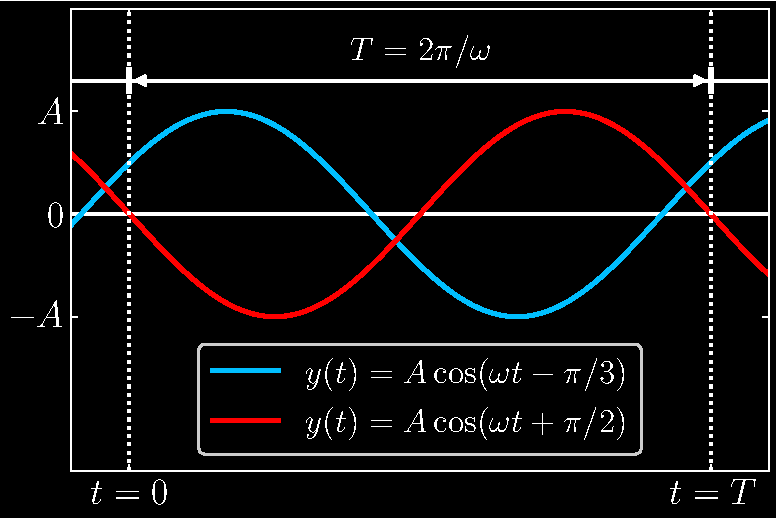
\includegraphics[width=1.0\textwidth]{../chap2/sec2.1/chap2sec2.1ex3.eps}
\end{center}

% QUESTION 4
\qs{2.1.4}{Suppose the circle in Figure 2.4 has radius 3 and circular frequency \(f = 60\) Hertz. If the moving point starts at the angle \(-45^{\circ}\), find its \(x\)-coordinate \(A \cos\left( \omega t - \alpha  \right)\). The phase lag is \(\alpha = 45^{\circ}\). When does the point first hit the \(x\)-axis?}

The circular motion of the point is expressed by the sinusoidal
\[
	3 \cos\left( 120 \pi t - \frac{\pi }{4} \right)
\]
Note that since the frequency is \(f = 60\) Hertz, the angular frequency is \(2 \pi \cdot 60 = 120 \pi \) radians s\(^{-1}\). The point hits the \(x\)-axis when the argument of the cosine is zero, namely at
\[
	120 \pi t - \frac{\pi }{4} = 0 \quad \implies \quad t = \frac{1}{480} \text{s}
\]

% QUESTION 5
\qs{2.1.5}{If you drive at 60 miles per hour on a circular track with radius \(R = 3\) miles, what is the time \(T\) for one complete circuit? Your circular frequency is \(f = \) \underline{\qquad} and your angular frequency is \(\omega = \) \underline{\qquad} (with what units?). The period is \(T\).}

Using dimensional analysis, the period is
\[
	T = \frac{1 \text{ hr}}{60 \text{ mi}} \!\left( 3 \text{ mi} \right) = \frac{1}{20} \text{ hr}
\]
The circular frequency is
\[
	f = \frac{60 \text{ mi}}{\text{ hr}} \frac{1 \text{ hr}}{3600 \text{ s}} \frac{1 \text{ cycle}}{3 \text{ mi}} = \frac{1}{180} \text{ s}^{-1}
\]
with angular frequency
\[
	\omega = 2 \pi f = \frac{\pi }{90} \text{ rad s}^{-1}
\]

% QUESTION 6
\qs{2.1.6}{The total energy \(E\) in the oscillating spring-mass system is
\begin{alignat*}{1}
	E & = \textbf{kinetic} \text{ energy in mass} + \textbf{potential} \text{ energy in spring} \\
	  & = \frac{m}{2} \!\left( \frac{d y}{d t}  \right)^{2} + \frac{k}{2}y^{2}
\end{alignat*}
Compute \(E\) when \(y = C \cos\left( \omega t \right) + D \sin\left( \omega t \right)\). The energy is constant!}

Given \(y \!\left( t \right) \), we have first time-derivative
\[
	\frac{d y}{d t} = - \omega C \sin\left( \omega t \right) + \omega D \cos\left( \omega t \right)
\]
squaring gives us
\[
	\!\left( \frac{d y}{d t}  \right)^{2} = \omega^{2} \!\left( C^{2} \sin^{2}\left( \omega t \right) - 2 CD \sin\left( \omega t \right) \cos\left( \omega t \right) + D^{2}\cos^{2}\left( \omega t \right) \right)
\]
Lastly, the \(y^{2}\) term is
\[
	y^{2} = C^{2} \cos^{2}\left( \omega t \right) + 2CD \sin\left( \omega t \right)\cos\left( \omega t \right) + D^{2}\sin^{2}\left( \omega t \right)
\]
Combining our ingredients, with \(\omega = \sqrt{k / m}\), observe that energy \(E\) reduces to a constant:
\begin{alignat*}{1}
	E & = \frac{m}{2} \!\left( \frac{d y}{d t}  \right)^{2} + \frac{k}{2} y^{2} \\
	  & = \frac{m}{2} \!\left( \frac{k}{m} \right) \!\left( C^{2}\sin^{2}\left( \omega t \right) - 2CD \sin\left( \omega t \right) \cos\left( \omega t \right) + D^{2} \cos^{2}\left( \omega t \right)\right)  \\ 
	  & \qquad + \frac{k}{2} \!\left( C^{2} \cos^{2}\left( \omega t \right) + 2CD \sin\left( \omega t \right)\cos\left( \omega t \right) + D^{2}\sin^{2}\left( \omega t \right) \right) \\
	  & = C^{2} + D^{2}
\end{alignat*}

\newpage

% QUESTION 7
\qs{2.1.7}{Another way to show that the total energy \(E\) is constant:

Multiply \(\bm{my'' + ky = 0}\) by \(\bm{y'}\). Then integrate \(my'y''\) and \(kyy'\).}

Take the first term and integrate:
\[
	m \int y'y'' \, dt
\]
By integration by parts, let
\[
	u = \frac{d y}{d t}, \quad \frac{d u}{d t} = \frac{d^{2}y}{d t^{2}} \quad \implies \quad du = \frac{d^{2}y}{d t^{2}} dt 
\]
Then we can rewrite the first term as
\[
	m \int u \, du = \frac{m}{2}u^{2} + C = \frac{m}{2} \!\left( y' \right)^{2} + C 
\]
as for the second term:
\[
	k \int yy' \, dt = k \int y \frac{d y}{d t}  \, dt = k \int y \, dy = \frac{k}{2}y^{2} + C 
\]
Summing the two pieces (sans the constants) restores the original energy function:
\[
	E = \frac{m}{2} \!\left( \frac{d y}{d t}  \right)^{2} + \frac{k}{2}y^{2}
\]
and since the derivative of a constant is zero, it must be the case that \(E\) is a constant.

\vspace{12pt}

% QUESTION 8
\qs{2.1.8}{A \textbf{forced oscillation} has another term in the equation and \(A \cos\left( \omega t \right)\) in the solution:
\[
	\frac{d^{2}y}{dt^{2}} + 4y = F \cos\left( \omega t \right) \quad \text{has} \quad y = C \cos\left( 2 t \right) + D \sin\left( 2 t \right) + A \cos\left( \omega t \right)
\]
\begin{enumerate}[label=(\alph*)]
	\item Substitute \(y\) into the equation to see how \(C\) and \(D\) disappear (they give \(y_{n}\). Find the forced amplitude \(A\) in the particular solution \(y_{p} = A \cos\left( \omega t \right)\).
	\item In case \(\omega = 2\) (forcing frequency \(=\) natural frequency), what answer does your formula give for \(A\)? The solution formula for \(y\) breaks down in this case.
\end{enumerate}}

The second time-derivative is
\[
	\frac{d^{2}y}{dt^{2}} = -4C \cos\left( 2t \right) - 4D \sin\left( 2t \right) - \omega^{2}A \cos\left( \omega t \right)
\]
\begin{enumerate}[label=(\alph*)]
	\item We have
		\[
			\frac{d^{2}y}{dt^{2}} + 4y = \!\left( 4 - \omega^{2} \right) A \cos\left( \omega t \right) = F \cos\left( \omega t \right)
		\]
	implying \(A = \dfrac{F}{4 - \omega^{2}}\).
	\item When \(\omega = 2\), \(A\) is undefined. 
\end{enumerate}

% QUESTION 9
\qs{2.1.9}{Following Problem 8, write down the complete solution \(y_{n} + y_{p}\) to the equation
\[
	m \frac{d^{2}y}{dt^{2}} + ky = F \cos\left( \omega t \right) \quad \text{with} \quad \omega \neq \omega_{n} = \sqrt{k / m} \quad \text{(no resonance)}
\]
The answer \(y\) has free constants \(C\) and \(D\) to match \(y \!\left( 0 \right) \) and \(y'\!\left( 0 \right) \) (\(A\) \textit{is fixed} by \(F\).}

Per Problem 8, we have solution
\[
	y = \underbrace{C \cos\left( \sqrt{\frac{k}{m}} t \right) + D \sin\left( \sqrt{\frac{k}{m}} t \right)}_{y_{n}} + \underbrace{\frac{F}{k - m \omega^{2}} \cos\left( \omega t \right)}_{y_{p}}
\]

All this involves is dividing the equation through by \(m\), understanding that the angular frequency of the sinusoidals in the null solution is the square root of \(k / m\), and making the changes to our formula for \(A\) accordingly.

\vspace{12pt}

% QUESTION 10
\qs{2.1.10}{Suppose Newton's Law \(F = ma\) has the force \(F\) in the \textit{same} direction as \(a\):
\[
	my'' = + ky \quad \text{including} \quad y'' = 4y
\]
Find two possible choices of \(s\) in the exponential solutions \(y = e^{st}\). The solution is not sinusoidal and \(s\) is real and the oscillations are gone. Now \(y\) is unstable.}

Substituting in \(y\), we find
\[
	ms^{2}e^{st} = ke^{st}
\]
This forces
\[
	s = \pm \sqrt{\frac{k}{m}}
\]
\newpage

% QUESTION 11
\qs{2.1.11}{Here is a \textit{fourth} order equation: \(d^{4}y / dt^{4} = 16y\). Find \textit{four} values of \(s\) that give exponential solutions \(y = e^{st}\). You could expect four initial conditions on \(y\): \(y \!\left( 0 \right) \) is given along with what three other conditions?}

Equivalently, we find the four complex roots of \(16\):
\[
	s^{4} = 16
\]
which are \(s = \pm 2, \pm 2i\).

\vspace{12pt}

% QUESTION 12
\qs{2.1.12}{To find a particular solution to \(y'' + 9y = e^{ct}\), I would look for a multiple \(y_{p}\!\left( t \right) = Ye^{ct}\) of the forcing function. What is that number \(Y\)? When does your formula give \(Y = \infty\)? (Resonance needs a new formula for \(Y\).)}

Let \(y_{p} = Ye^{ct}\). Substituting, we find
\[
	Yc^{2} e^{ct} + 9Ye^{ct} = e^{ct}
\]
Solving for \(Y\) yields \(Y = \dfrac{1}{c^{2} + 9}\). When \(c \rightarrow \pm3\), we have resonance, and \(Y \rightarrow \infty\).

\vspace{12pt}

% QUESTION 13
\qs{2.1.13}{In a particular solution \(y = Ae^{i \omega t}\) to \(y'' + 9y = e^{i \omega t}\), what is the amplitude \(A\)? The formula blows up when the forcing frequency \(\omega =\) what natural frequency?}

Substituting, we derive
\[
	-\omega^{2}A e^{i \omega t} + 9A e^{i \omega t} = e^{i \omega t}
\]
which gives us \(A = \dfrac{1}{9 - \omega^{2}}\). Resonance is when \(\omega = 3\).

\vspace{12pt}

\newpage
% QUESTION 14
\qs{2.1.14}{Equation (10) says that the tangent of the phase angle is \(\tan\left( \alpha  \right) = y' \!\left( 0 \right) / \omega y \!\left( 0 \right) \). First, check that \(\tan\left( \alpha  \right)\) is dimensionless when \(y\) is in meters and time is in seconds. Next, if that ratio is \(\tan\left( \alpha  \right) = 1\), should you choose \(\alpha = \pi / 4\) or \(\alpha = 5 \pi / 4\)? Answer:
\[
	\text{Separately you want } R \cos \left( \alpha  \right) = y \!\left( 0 \right)  \text{ and } R \sin \left( \alpha  \right) = y' \!\left( 0 \right) / \omega 
\]
If those right hand sides are positive, choose the angle \(\alpha \) between \(0\) and \(\pi / 2\). 

If those right hand sides are negative, add \(\pi \) and choose \(\alpha = 5 \pi / 4\).

\vspace{12pt}

\textit{Question}: If \(y \!\left( 0 \right) > 0\) and \(y' \!\left( 0 \right) < 0\), does \(\alpha \) fall between \(\pi / 2\) and \(\pi \) or between \(3 \pi / 2\) and \(2 \pi \)? If you plot the vector from \( \!\left( 0, 0 \right) \) to \(\!\left( y \!\left( 0 \right) , y' \!\left( 0 \right) / \omega  \right) \), its angle is \(\alpha \).}

As \(y \!\left( 0 \right) > 0\) and \(y'\!\left( 0 \right) < 0\) requires positive cosine and negative sine, \(\alpha \) falls between \(3 \pi / 2\) and \(2 \pi \).

\vspace{12pt}

% QUESTION 15
\qs{2.1.15}{Find a point on the sine curve in Figure 2.1 where \(y > 0\) but \(v = y' < 0\) and also \(a = y'' < 0\). The curve is sloping down and bending down.

\vspace{12pt}

Find a point where \(y < 0\) but \(y' > 0\) and \(y'' > 0\). The point is below the \(x\)-axis but the curve is sloping \underline{\qquad} and bending \underline{\qquad}.}

One area corresponding to the first set of conditions is \(\pi / 2 < t < \pi \). As for the second, we have \(3 \pi / 2 < t < 2 \pi \).

\vspace{12pt}

% QUESTION 16
\qs{2.1.16}{
\begin{enumerate}[label=(\alph*)]
	\item Solve \(y'' + 100y = 0\) starting from \(y \!\left( 0 \right) = 1\) and \(y' \!\left( 0 \right) = 10\). (\( \textbf{This is } \bm{y_{n}} \).)
	\item Solve \(y'' + 100y = \cos\left( \omega t \right)\) with \(y \!\left( 0 \right) = 0\) and \(y' \!\left( 0 \right) = 0\). (\( \textbf{This can be }\bm{y_{p}} \).)
\end{enumerate}}

\begin{enumerate}[label=(\alph*)]
	\item Let \(y = c_{1} \cos\left( 10 t \right) + c_{2} \sin\left( 10 t \right)\). Then \(y \!\left( 0 \right) = c_{1} = 1\) and \(y' \!\left( 0 \right) = 10 c_{2} = 10\) implies \(c_{2} = 1\). Then the null solution is
	\[
		y_{n} = \cos\left( 10 t \right) + \sin\left( 10 t \right)
	\]
\item Let \(y_{p} = R \cos\left( \omega t \right)\). Substitute to find
	\[
		-\omega^{2} R \cos\left( \omega t \right) + 100 R \cos\left( \omega t \right) = \cos\left( \omega t \right)
	\]
	Isolate \(R\) to derive
	\[
		R = \frac{1}{100 - \omega^{2}}
	\]
	The solution to this set of initial conditions requires \(y \!\left( 0 \right) = 0 \) and \(y' \!\left( 0 \right) = 0\). Begin with
	\[
		y \!\left( t \right) = c_{1} \cos\left( 10 t \right) + c_{2} \sin\left( 10 t \right) + \frac{1}{100 - \omega^{2}} \cos\left( \omega t \right)	
	\]
	From the first condition, we have \(c_{1} = -\dfrac{1}{100 - \omega^{2}}\). From the second, we have \(c_{2} = 0\). The full solution is
	\[
		y \!\left( t \right) = \frac{1}{100 - \omega^{2}} \!\left( \cos\left( \omega t \right) - \cos\left( 10t \right) \right) 
	\]
\end{enumerate}

% QUESTION 17
\qs{2.1.17}{Find a particular solution \(y_{p} = R \cos\left( \omega t - \alpha  \right)\) to \(y'' + 100y = \cos\left( \omega t \right) - \sin\left( \omega t \right)\).}

Substituting \(y_{p}\) gives us

\begin{alignat*}{2}
	& -\omega^{2} R \cos\left( \omega t - \alpha  \right) + 100 R \cos\left( \omega t - \alpha  \right) \\
		 & \qquad = \!\left( 100R - \omega^{2}R \right) \!\left[ \cos\left( \omega t \right)\cos\left( \alpha  \right) + \sin\left( \omega t \right)\sin\left( \alpha  \right) \right]  \\
\end{alignat*}

This implies that
\begin{alignat*}{1}
	R \cos\left( \alpha  \right) \!\left( 100 - \omega^{2} \right) & = 1 \\
	R \sin\left( \alpha  \right) \!\left( 100 - \omega^{2} \right) & = -1 \\ 
\end{alignat*}
enabling us to conclude that \(\alpha = 7 \pi / 4\), and amplitude
\[
	R = \frac{\sqrt{2}}{100 - \omega^{2}}
\]
Ergo, the particular solution is
\[
	y_{p} = \frac{\sqrt{2}}{100 - \omega^{2}} \cos\left( \omega t - \frac{7 \pi }{4} \right)
\]

% QUESTION 18
\qs{2.1.18}{Simple harmonic motion also comes from a linear pendulum (like a grandfather clock). At time \(t\), the height is \(A \cos\left( \omega t \right)\). What is the frequency \(\omega \) if the pendulum comes back to the start after 1 second? The period does not depend on the amplitude (a large clock or a small metronome or the movement in a watch can all have \(T = 1\)).}

The angular frequency is \(2 \pi \cdot f = 2 \pi \) radians s\(^{-1}\).

\vspace{12pt}

% QUESTION 19
\qs{2.1.19}{If the phase lag is \(\alpha \), what is the time lag in graphing \(\cos\left( \omega t - \alpha \right)\)?}

Put differently, we want to find the value of \(t'\) such that we are able to restore \(\omega t\) as the cosine's argument. If we have
\[
	t' = t + \alpha / \omega 
\]
then we get
\[
	\cos\left( \omega t' - \alpha  \right) = \cos\left( \omega \!\left( t + \alpha / \omega  \right) - \alpha  \right) = \cos\left( \omega t \right)
\]
Thus the time lag term is \(\alpha / \omega \).

\vspace{12pt}

% QUESTION 20
\qs{2.1.20}{What is the response \(y \!\left( t \right) \) to a delayed impulse if \(my'' + ky = \delta \!\left( t - T \right) \)?}

The full solution will be a factor of the step function, given by:
\[
	y \!\left( t \right) = \int^{t - T}_{0} \frac{\sin\left( \omega_{n} \!\left( t - T - s \right)  \right)}{m \omega_{n}} \delta \!\left( s \right)  \, ds = \frac{\sin\left( \omega_{n} \!\left( t - T \right)  \right)}{m \omega_{n}} H \!\left( t - T \right) 
\]
Intuitively, when \(t \le T\), the right-hand side vanishes. No impulse is imparted, and thus there is no response. But when we are at time \(t \ge T\) -- after the threshold -- the response kicks in.
\vspace{12pt}

% QUESTION 21
\qs{2.1.21}{(Good challenge) Show that \(\displaystyle{y = \int^{t}_{0} g \!\left( t - s \right) f \!\left( s \right)  \, ds }\) has \(my'' + ky = f \!\left( t \right) \).

\begin{enumerate}[label=\arabic*.]
	\item Why is \(\displaystyle{y' = \int^{t}_{0} g'\!\left( t - s \right) f \!\left( s \right)  \, ds + g \!\left( 0 \right) f \!\left( t \right)  }\)? Notice the two \(t\)'s in \(y\).
	\item Using \(g \!\left( 0 \right) = 0\), explain why \(\displaystyle{y'' = \int^{t}_{0} g''\!\left( t - s \right) f \!\left( s \right)  \, ds + g'\!\left( 0 \right) f \!\left( t \right)  }\).
	\item Now use \(g'\!\left( 0 \right) = 1 / m\) and \(mg'' + kg = 0\) to confirm \(my'' + ky = f \!\left( t \right) \).
\end{enumerate}}

Use the Leibniz integral rule:
\[
	\frac{d }{d t} \!\left( \int^{t}_{0} g \!\left( t - s \right) f \!\left( s \right)  \, ds \right) = g\!\left( 0 \right) f \!\left( t \right) + \int^{t}_{0} \frac{\partial }{\partial t} g \!\left( t - s \right) f \!\left( s \right)  \, ds 
\]

\begin{enumerate}[label=(\arabic*)]
	\item By above, applying the partial derivative inside the second term yields the desired result.
	\item One more application of the Leibniz rule gives us
	\[
		y'' = \int^{t}_{0} g''\!\left( t - s \right) f \!\left( s \right)  \, ds + g \!\left( 0 \right) f'\!\left( t \right) + g'\!\left( 0 \right) f \!\left( t \right) 
	\]
	With the premise \(g \!\left( 0 \right) = 0\), the second term vanishes and gives us the expected result.
	\item Derive
	\[
		my'' + ky = \int^{t}_{0} \!\left[ mg''\!\left( t - s \right) + kg \!\left( t - s \right)  \right] f \!\left( s \right)  \, ds + f \!\left( t \right) = f \!\left( t \right)   \\
	\]
	where the last equality follows by appealing to the nullity of \(g \!\left( t \right) \).
\end{enumerate}

% QUESTION 22
\qs{2.1.22}{With \(f = 1\) (direct current has \(\omega = 0\)) verify that \(my'' + ky = 1\) for this \(y\):
\[
	\textbf{Step response}
\]
\[
	y \!\left( t \right) = \int^{t}_{0} \frac{\sin\left( \omega_{n} \!\left( t - s \right)  \right)}{m \omega_{n}} \cdot 1 \, ds = y_{p} + y_{n} = \pmb{\frac{1}{k} - \frac{1}{k} \cos\left( \omega_{n}t \right)}
\]}

We have second derivative
\[
	y''\!\left( t \right) = \frac{\omega_{n}^{2}}{k}\cos\left( \omega_{n}t \right)	
\]
Since \(\omega_{n} = \sqrt{k / m}\), \(my''\!\left( t \right) = \cos\left( \omega_{n}t \right)\). Ergo, we have
\[
	my'' + ky = \cos\left( \omega_{n}t \right) + k \!\left[ \frac{1}{k} - \frac{1}{k}\cos\left( \omega_{n}t \right) \right] = 1
\]

% QUESTION 23
\qs{2.1.23}{(Recommended) For the equation \(d^{2}y / dt^{2} = 0\) find the null solution. Then for \(d^{2}g / dt^{2} = \delta \!\left( t \right) \) find the fundamental solution (start the null solution with \(g \!\left( 0 \right) = 0\) and \(g'\!\left( 0 \right) = 1\)). For \(y'' = f \!\left( t \right) \) find the particular solution using formula (16).}

Integrating twice, the null solution is
\[
	y \!\left( t \right) = C_{1} t + C_{2}
\]
To find the fundamental solution \(g \!\left( t \right) \), imposing the initial conditions \(g \!\left( 0 \right) = 0\) and \(g'\!\left( 0 \right) = 1\) forces \(C_{1} = 1\) and \(C_{2} = 0\), thus
\[
	g \!\left( t \right) = t
\]
Lastly, if \(y'' = f \!\left( t \right) \), then
\[
	y_{p}\!\left( t \right) = \int^{t}_{0} \!\left( t - s \right) f \!\left( s \right)  \, ds 
\]
% QUESTION 24
\qs{2.1.24}{For the equation \(d^{2}y/ dt^{2} = e^{i \omega t}\) find a particular solution \(y = Y \!\left( \omega  \right) e^{i \omega t}\). Then \(Y \!\left( \omega  \right) \) is the frequency response. Note the ``resonance'' when \(\omega = 0\) with the null solution \(y_{n} = 1\).}

One particular solution is
\[
	y \!\left( t \right) = -\frac{e^{i \omega t}}{\omega^{2}}
\]
meaning that \(Y \!\left( \omega  \right) = - 1 / \omega^{2}\). When \(\omega = 0\), we have resonance, and this particular solution breaks down.

\vspace{12pt}

% QUESTION 25
\qs{2.1.25}{Find a particular solution \(Ye^{i \omega t}\) to \(my'' - ky = e^{i \omega t}\). The equation has \(-ky\) instead of \(ky\). What is the frequency response \(Y \!\left( \omega  \right) \)? For which \(\omega \) is \(Y\) infinite?}

We have
\[
	\frac{d^{2} }{d t^{2}} \!\left( Y e^{i \omega t} \right) = - Y \omega^{2} e^{i \omega t}
\]
Substituting and canceling the \(e^{i \omega t}\) terms, we get
\[
	-mY \omega^{2} - kY = 1
\]
Implying
\[
	Y \!\left( \omega  \right) = -\frac{1}{m \omega^{2} + k}
\]
If we have
\[
	\omega = i \sqrt{\frac{k}{m}}
\]
then \(Y \!\left( \omega  \right) \) diverges to infinity -- meaning all real frequencies will not lead to this!

\newpage

\subsection{\textsf{2.2 - Key Facts About Complex Numbers}}

% QUESTION 1
\qs{2.2.1}{Mark the numbers \(s_{1} = 2 + i\) and \(s_{2} = 1 - 2i\) as points in the complex plane. (The plane has a real axis and an imaginary axis.) Then mark the sum \(s_{1} + s_{2}\) and the difference \(s_{1} - s_{2}\).}

Arithmetic involving complex numbers simply is vector superposition:

\begin{center}
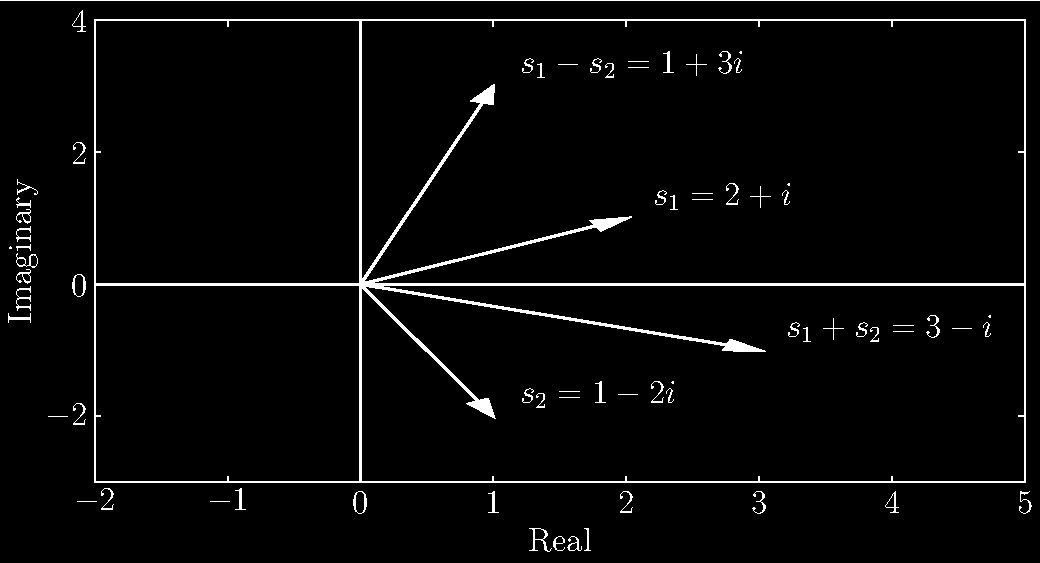
\includegraphics[width=1.0\textwidth]{../chap2/sec2.2/chap2sec2.2ex1.eps}
\end{center}

\vspace{12pt}

% QUESTION 2
\qs{2.2.2}{Multiply \(s_{1} = 2 + i\) times \(s_{2} = 1 - 2i\). Check absolute values: \(\abs{s_{1}} \abs{s_{2}} = \abs{s_{1}s_{2}}\).}

We have
\[
	\!\left( 2 + i \right) \!\left( 1 - 2i \right) = 2 - 4i + i + 2 = 4 - 3i
\]
with \(\abs{s_{1}} = \abs{s_{2}} = \sqrt{5}\), \(\abs{s_{1}s_{2}} = \sqrt{16 + 9} = 5\), ascertaining \(\abs{s_{1}}\abs{s_{2}} = \abs{s_{1}s_{2}}\).

\vspace{12pt}

% QUESTION 3
\qs{2.2.3}{Find the real and imaginary parts of \(1 / \!\left( 2 + i \right) \). 

Multiply by \(\!\left( 2 - i \right) / \!\left( 2 - i \right) \):
\[
	\frac{1}{2 + i} \frac{2 - i}{2 - i} = \frac{2 - i}{\abs{2 + i}^{2}} = \quad ?
\]
}

The denominator is \(5\), so we have
\[
	\underbrace{\frac{2}{5}}_{\text{real}} - \underbrace{\frac{i}{5}}_{\text{imaginary}}
\]

% QUESTION 4
\qs{2.2.4}{\textit{Triple angles} \quad Multiply equation (10) by another \(e^{i \theta } = \cos\left( \theta  \right) + i \sin\left( \theta  \right)\) to find formulas for \(\cos\left( 3 \theta  \right)\) and \(\sin\left( 3 \theta  \right)\).}

Derive
\begin{alignat*}{1}
	\!\left( \cos\left( \theta  \right) + i \sin\left( \theta  \right) \right)^{3} & = \!\left( \cos^{2}\left( \theta  \right) - \sin^{2}\left( \theta  \right) + 2i \cos\left( \theta  \right) \sin\left( \theta  \right) \right) \!\left( \cos\left( \theta  \right) + i \sin\left( \theta  \right) \right)  \\
	 & = \cos^{3}\left( \theta  \right) - \sin^{2}\left( \theta  \right) \cos\left( \theta  \right) + 2i \cos^{2}\left( \theta  \right) \sin\left( \theta  \right) \\ 
	 & \qquad + i \cos^{2}\left( \theta  \right) \sin\left( \theta  \right) - i \sin^{3}\left( \theta  \right) - 2 \cos\left( \theta  \right) \sin^{2}\left( \theta  \right) \\
	 & = \underbrace{\cos^{3}\left( \theta  \right) - 3 \sin^{2}\left( \theta  \right) \cos\left( \theta  \right) }_{\text{real}} + i \underbrace{\!\left[ 3 \cos^{2}\left( \theta  \right) \sin\left( \theta  \right) - \sin^{3}\left( \theta  \right) \right] }_{\text{imaginary}}
\end{alignat*}

% QUESTION 5
\qs{2.2.5}{\textit{Addition formulas} Multiply 
\(e^{i \theta } = \cos\left( \theta  \right) + i \sin\left( \theta  \right)\) times \(e^{i \phi } = \cos\left( \phi  \right) + i \sin\left( \phi  \right)\) to get \(e^{i \!\left( \theta + \phi  \right) }\). Its real part is \(\cos\left( \theta + \phi  \right) = \cos\left( \theta  \right) \cos\left( \phi  \right) - \sin\left( \theta  \right) \sin\left( \phi  \right)\). What is its imaginary part \(\sin\left( \theta + \phi  \right)\)?}

Derive
\begin{alignat*}{1}
	\!\left[ \cos\left( \theta  \right) + i \sin\left( \theta  \right) \right] \!\left[ \cos\left( \phi  \right) + i \sin\left( \phi  \right) \right]  & = \underbrace{\cos\left( \theta  \right)\cos\left( \phi  \right) - \sin\left( \theta  \right)\sin\left( \phi  \right)}_{\text{real}} \\
																			   & \qquad + i \underbrace{\!\left[ \cos\left( \theta  \right) \sin\left( \phi  \right) + \sin\left( \theta  \right) \cos\left( \phi  \right) \right]}_{\text{imaginary}}  \\
\end{alignat*}

% QUESTION 6
\qs{2.2.6}{Find the real part and the imaginary part of each cube root of 1. Show directly that the three roots add to zero, as equation (11) predicts.}

The cube roots, in polar form, are given by
\begin{alignat*}{1}
	e^{i 2 \pi / 3} & = -\frac{1}{2} + i \frac{\sqrt{3}}{2} \\
	e^{i 4 \pi / 3} & = -\frac{1}{2} - i \frac{\sqrt{3}}{2}\\
	 & \qquad 1 
\end{alignat*}

which vanish when summed.

\newpage

% QUESTION 7
\qs{2.2.7}{The three cube roots of 1 are \(z\) and \(z^{2}\) and 1, when \(z = e^{2 \pi i / 3}\). What are the three cube roots of 8 and the three cube roots of \(i\)? (The angle for \(i\) is \(90^{\circ}\) or \(\pi / 2\), so the angle for one of its cube roots will be \underline{\qquad}. The roots are spaced by \(120^{\circ}\).}

In polar form, we can express 8 as \(8e^{2 \pi i}\). Let \(z = e^{2 \pi i / 3}\). Its cube roots are then \(2z\), \(2z^{2}\), and \(2\). 

For \(i\), we have polar form \(e^{\pi i / 2}\). Then its cube roots are \(e^{\pi i / 6}\), \(e^{5 \pi i / 6}\), and \(e^{3 \pi i / 2}\). 

Argue by vector superposition that the cube roots in all cases sum to zero.

\vspace{12pt}

% QUESTION 8
\qs{2.2.8}{
	\begin{enumerate}[label=(\alph*)]
	\item The number \(i\) is equal to \(e^{\pi i / 2}\). Then its \(i^{\text{th}}\) power \(i^{i}\) comes out equal to a real number, using the fact that \(\!\left( e^{s} \right)^{t} = e^{st}\). What is that real number \(i^{i}\)?
	\item \(e^{i \pi / 2}\) is also equal to \(e^{5 \pi i / 2}\). Increasing the angle by \(2 \pi \) does not change \(e^{i \theta }\) - it comes around a full circle and back to \(i\). Then \(i^{i}\) has another real value \(\!\left( e^{5 \pi i / 2} \right)^{i} = e^{-5 \pi / 2}\). What are all the possible values of \(i^{i}\)?
\end{enumerate}}

\begin{enumerate}[label=(\alph*)]
	\item We have \(\!\left( e^{\pi i / 2} \right)^{i} = e^{-\pi / 2}\).
	\item All possible values of \(i^{i}\) are \(e^{\!\left( - \pi \pm 4n \pi  \right) / 2}\).
\end{enumerate}

% QUESTION 9
\qs{2.2.9}{The numbers \(s = 3 + i\) and \(\overline{s} = 3 - i \) are complex conjugates. Find their sum \(s + \overline{s} = -B\) and their product \(\!\left( s \right) \!\left( \overline{s} \right) = C\). Then show that \(s^{2} + Bs + C = 0\) and also \(\overline{s}^{2} + B \overline{s} + C = 0\). Those numbers \(s\) and \(\overline{s}\) are the two roots of the quadratic equation \(x^{2} + Bx + C = 0\).}

The sum is \(s + \overline{s} = 6\), so \(B = -6\). Their product is \(s \overline{s} = 10 = C\). Then we have
\[
	s^{2} + Bs + C = s^{2} - \!\left( s + \overline{s} \right) s + s \overline{s} = 0
\]
\[
	\overline{s}^{2} + B \overline{s} + C = \overline{s}^{2} - \!\left( s + \overline{s} \right) \overline{s} + s \overline{s} = 0
\]

% QUESTION 10
\qs{2.2.10}{The numbers \(s = a + i \omega \) and \(\overline{s} = a - i \omega \) are complex conjugates. Find their sum \(s + \overline{s} = -B\) and their product \(\!\left( s \right) \!\left( \overline{s} \right) = C\). Then show that \(s^{2} + Bs + C = 0\). The two solutions of \(x^{2} + Bx + C = 0\) are \(s\) and \(\overline{s}\).}

The sum is \(s + \overline{s} = 2a\), so \(B = -2a\). Their product is \(s \overline{s} = a^{2} + \omega^{2}\). By the same argument as the previous problem, the solutions of the given polynomial are \(s\) and \(\overline{s}\).

\vspace{12pt}

% QUESTION 11
\qs{2.2.11}{\begin{enumerate}[label=(\alph*)]
	\item Find the numbers \(\!\left( 1 + i \right)^{4} \) and \(\!\left( 1 + i \right)^{8}\).
	\item Find the polar form \(re^{i \theta }\) of \(\!\left( 1 + i \sqrt{3} \right) / \!\left( \sqrt{3} + i \right) \).
\end{enumerate}}

\begin{enumerate}[label=(\alph*)]
	\item We have \(1 + i = \sqrt{2} e^{i \pi / 4}\). Then
	\[
		\!\left( \sqrt{2} e^{i \pi / 4} \right)^{4} = 4 e^{i \pi } = -4
	\]
	Raising to the eighth power, we simply square our previous answer to get \(\!\left( 1 + i \right)^{8} = 16\).
	\item The numerator is \(2e^{i \pi / 3}\) and the denominator \(2 e^{i \pi / 6}\). The quotient is \(e^{i \pi / 6}\).
\end{enumerate}

% QUESTION 12
\qs{2.2.12}{The number \(z = e^{2 \pi i / n}\) solves \(z^{n} = 1\). The number \(Z = e^{2 \pi i / 2n}\) solves \(Z^{2n} = 1\). How is \(z\) related to \(Z\)? (This plays a big part in the Fast Fourier Transform.)}

They are related by \(z = Z^{2}\).

\vspace{12pt}

% QUESTION 13
\qs{2.2.13}{\begin{enumerate}[label=(\alph*)]
	\item If you know \(e^{i \theta }\) and \(e^{-i \theta }\), how can you find \(\sin\left( \theta  \right)\)?
	\item Find all angles \(\theta \) with \(e^{i \theta } = -1\) and all angles \(\phi \) with \(e^{i \phi } = -i\).
\end{enumerate}}

\begin{enumerate}[label=(\alph*)]
	\item One way to write \(\sin\left( \theta  \right)\) is
	\[
		\frac{e^{i \theta } - e^{-i \theta }}{2} = \sin\left( \theta  \right)
	\]
\item We have \(\theta = \pi \pm 2n \pi \) (which eliminates the imaginary term), and \(\phi = - \frac{\pi }{2} \pm 2n \pi \). 
\end{enumerate}

\newpage
% QUESTION 14
\qs{2.2.14}{Locate all these points on one complex plane:
\begin{enumerate}[label=(\alph*)]
	\item \(2 + i\)
	\item \( \!\left( 2 + i \right)^{2} \)
	\item \(\displaystyle{\frac{1}{2 + i}}\)
	\item \(\abs{2 + i}\)
\end{enumerate}}

\begin{enumerate}[label=(\alph*)]
	\item \(2 + i\)
	\item \(\!\left( 2 + i \right)^{2} = 3 + 4i\)
	\item \(\displaystyle{\frac{1}{2 + i}} = \frac{2 - i}{5}\)
	\item \(\abs{2 + i} = \sqrt{5}\)
\end{enumerate}

\begin{center}
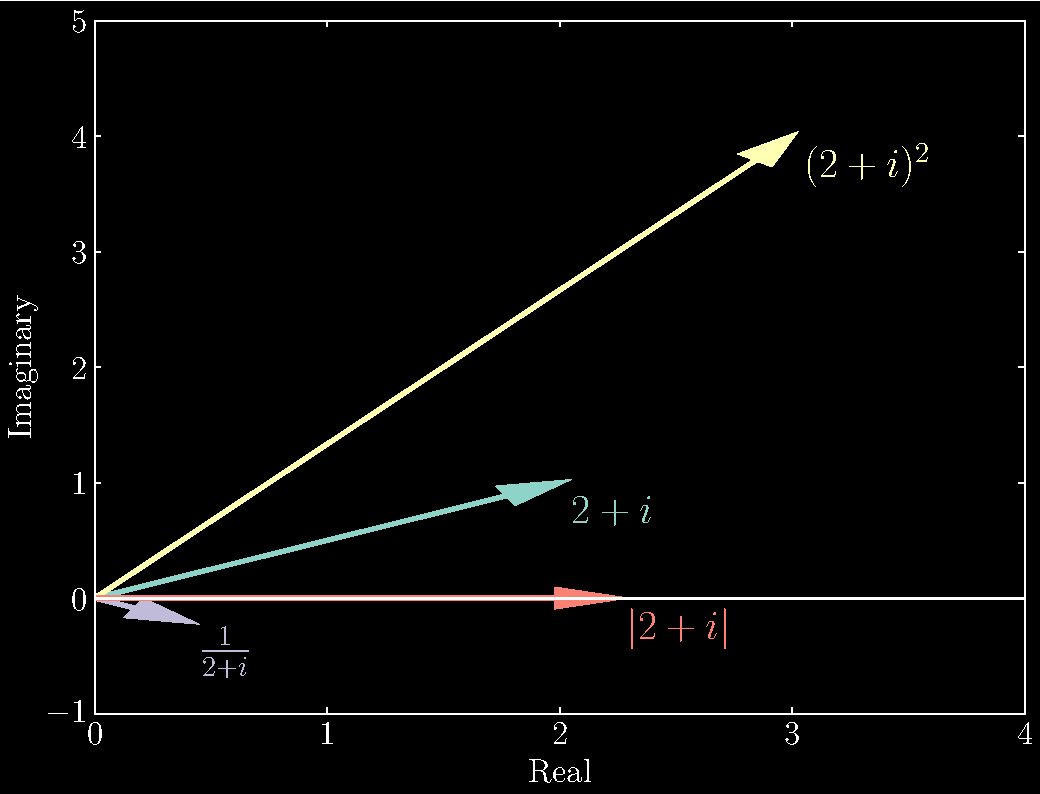
\includegraphics[width=1.0\textwidth]{../chap2/sec2.2/chap2sec2.2ex14.eps}
\end{center}

\newpage
% QUESETION 15
\qs{2.2.15}{Find the absolute values \(r = \abs{z}\) of these four numbers. If \(\theta \) is the angle for \(6 + 8i\), what are the angles for these four numbers?
\begin{enumerate}[label=(\alph*)]
	\item \(6 - 8i\)
	\item \(\!\left( 6 - 8i \right)^{2}\)
	\item \(\displaystyle{\frac{1}{6 - 8i}}\)
	\item \(8i + 6\)
\end{enumerate}}

\begin{enumerate}[label=(\alph*)]
	\item \(r = 10\), \(\phi = -\theta \), in polar form \(z = 10e^{-i \theta }\)
	\item \(r = 100\), \(\phi = -2 \theta \), in polar form \(z = 100e^{-2 \theta }\)
	\item \(r = 1 / 10\), \(\phi = \theta \), in polar form \(\displaystyle{z = \frac{1}{10} e^{i \theta }}\)
	\item \(r = 10\), \(\phi = \theta \), the original number is unchanged
\end{enumerate}

% QUESTION 16
\qs{2.2.16}{What are the real and imaginary parts of \(e^{a + i \pi }\) and \(e^{a + i \omega }\)?}

The real parts are \(-e^{a}\) and \(e^{a} \cos\left( \omega  \right)\) and the imaginary parts are \(0\) and \(e^{a} \sin\left( \omega  \right)\).

\vspace{12pt}

% QUESTION 17
\qs{2.2.17}{\begin{enumerate}[label=(\alph*)]
	\item If \(\abs{s} = 2\) and \(\abs{z} = 3\), what are the absolute values of \(sz\) and \(s / z\)?
	\item Find upper and lower bounds in \(L \le \abs{s + z} \le U\). When does \(\abs{s + z} = U\)?
\end{enumerate}}

\begin{enumerate}[label=(\alph*)]
	\item \(\abs{sz} = \abs{s}\abs{z} = 6\), \(\abs{s / z} = \abs{s}/\abs{z} = 2/3\)
	\item The lower bound is achieved when \(s\) and \(z\) are antiparallel, meaning the modulus of their vector sum is at best \(L = \abs{s + z} = 1\). The upper bound is reached when they are parallel, so \(U = \abs{s + z} = 5\).
\end{enumerate}

\newpage
% QUESTION 18
\qs{2.2.18}{
\begin{enumerate}[label=(\alph*)]
	\item Where is the product \(\!\left( \sin\left( \theta  \right) + i \cos\left( \theta  \right) \right) \!\left( \cos\left( \theta  \right) + i \sin\left( \theta  \right) \right) \) in the complex plane?
	\item Find the absolute value  \(\abs{S}\) and the polar angle \(\phi \) for \(S = \pmb{\sin\left( \theta  \right) + i \cos\left( \theta  \right)}\).
\end{enumerate}
This is my favorite problem, because \(S\) combines \(\cos\left( \theta  \right)\) and \(\sin\left( \theta  \right)\) in a new way. To find \(\phi \), you could plot \(S\) or add angles in the multiplication of part (a).}

\begin{enumerate}[label=(\alph*)]
	\item Note that \(\sin\left( \theta  \right) = \displaystyle{\cos\left( \frac{\pi }{2} - \theta  \right)}\) and \(\cos\left( \theta  \right) = \displaystyle{\sin\left( \frac{\pi }{2} - \theta  \right)}\). Then the first term is equal to \(\displaystyle{\cos\left( \frac{\pi }{2} - \theta  \right) + i \sin\left( \frac{\pi }{2} - \theta  \right) = e^{i \!\left( \pi / 2 - \theta  \right) }}\). Then the product is
	\[
		e^{i \!\left( \pi / 2 - \theta  \right) } e^{i \theta } = e^{i \pi / 2} = i
	\]
	\item \(\abs{S} = 1\) and \(\displaystyle{\phi = \frac{\pi }{2} - \theta }\).
\end{enumerate}

% QUESTION 19
\qs{2.2.19}{Draw the spirals \(e^{\!\left( 1 - i \right)t}\) and \(e^{\!\left( 2 - 2i \right)t}\). Do those follow the same curves? Do they go clockwise or anticlockwise? When the first one reaches the negative \(x\)-axis, what is the time \(T\)? What point has the second one reached at that time?}

As \(t \rightarrow \infty\), the spirals progress clockwise. When the imaginary part vanishes, we have \(T = \pi \), and \(e^{\!\left( 1 - i \right) \pi } = e^{\pi }\). At that point in time, we also have \(e^{\!\left( 2 - 2i \right) \pi } = e^{2 \pi }\).

\begin{center}
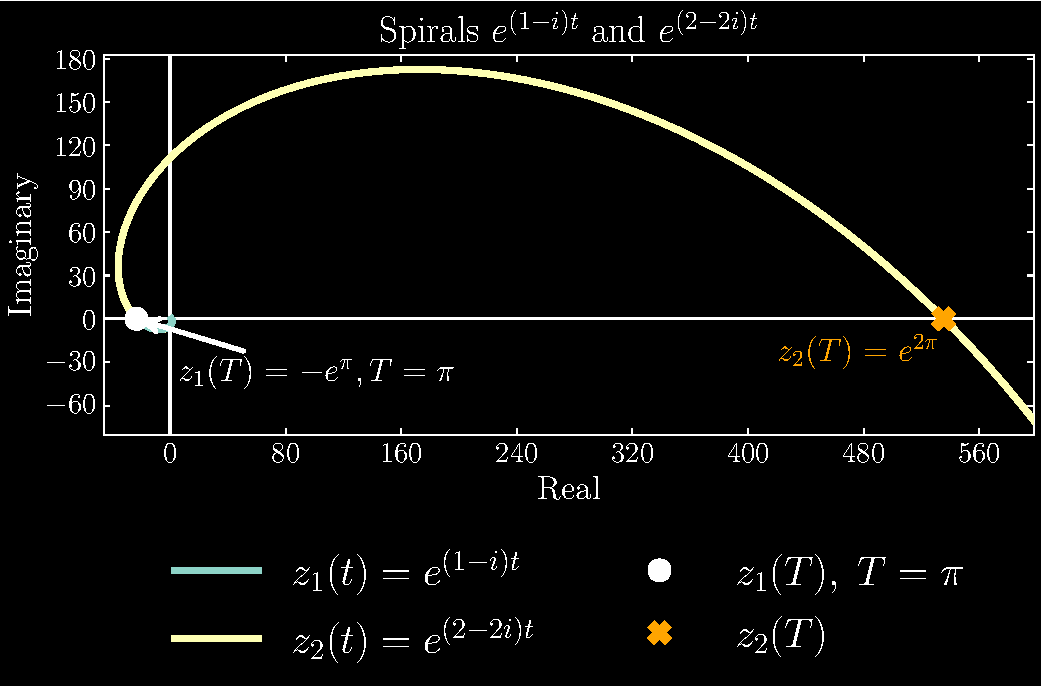
\includegraphics[width=1.0\textwidth]{../chap2/sec2.2/chap2sec2.2ex19.eps}
\end{center}

% QUESTION 20
\qs{2.2.20}{The solution to \(d^{2}y / dt^{2} = -y\) is \(y = \cos\left( t \right)\) if the initial conditions are \(y \!\left( 0 \right) = \underline{\qquad}\) and \(y' \!\left( 0 \right) = \underline{\qquad}\). The solution is \(y = \sin\left( t \right)\) when \(y \!\left( 0 \right) = \underline{\qquad}\) and \(y'\!\left( 0 \right) = \underline{\qquad}\). Write each of those solutions in the form \(c_{1}e^{i t} + c_{2}e^{-i t}\), to see that real solutions can come from complex \(c_{1}\) and \(c_{2}\).}

For the case of \(y = \cos\left( t \right)\), the initial conditions are \(y \!\left( 0 \right) = 1\) and \(y'\!\left( 0 \right) = 0\). In the case of \(y  = \sin\left( t \right)\), we have \(y \!\left( 0 \right) = 0\) and \(y'\!\left( 0 \right) = 1\). In the given form, the initial conditions require

\underline{\(y = \cos\left( t \right)\)}
\begin{align*}
	y \!\left( 0 \right) & = c_{1} + c_{2} = 1 \\
	y' \!\left( 0 \right) & = i \!\left( c_{1} - c_{2} \right) = 0
\end{align*}
Implying \(c_{1} = c_{2} = 1/2\).

\underline{\( y = \sin\left( t \right) \)}
\begin{align*}
	y \!\left( 0 \right)  & = c_{1} + c_{2} = 0 \\
	y'\!\left( 0 \right)  & = i \!\left( c_{1} - c_{2} \right) = 1  
\end{align*}
Implying \(c_{1} = 1 / 2i\) and \(c_{2} = -1 / 2i\).

Thus we can write \(\cos\left( t \right)\) and \(\sin\left( t \right)\) as
\[
	\cos\left( t \right) = \frac{e^{i t} + e^{-i t}}{2}, \quad \sin\left( t \right) = \frac{e^{i t} - e^{-i t}}{2i}
\]

The general solution is given by
\[
	y \!\left( t \right) = C_{1} \cos\left( t \right) + C_{2} \sin\left( t \right)
\]
which we rewrite as
\begin{align*}
	y \!\left( t \right)  & = C_{1} \cos\left( t \right) + C_{2} \sin\left( t \right) \\
	 & = C_{1} \!\left[ \frac{e^{i t} + e^{-i t}}{2} \right] + C_{2} \!\left[ \frac{e^{i t} - e^{-i t}}{2i} \right]   \\ 
	 & = \!\left[ \frac{C_{1} - iC_{2}}{2} \right] e^{i t} + \!\left[ \frac{C_{1} + iC_{2}}{2} \right] e^{-i t}
\end{align*}

% QUESTION 21
\qs{2.2.21}{Suppose \(y \!\left( t \right) = e^{-t}e^{i t}\) solves \(y'' + By' + Cy = 0\). What are \(B\) and \(C\)? If this equation is solved by \(y = e^{3it}\), what are \(B\) and \(C\)?}

Note that \(y \!\left( t \right) = e^{-t}e^{i t} = e^{\!\left( -1 + i \right) t}\). Then we have
\[
	y'' + By' + Cy = \!\left( -1 + i \right)^{2} e^{\!\left( -1 + i \right) t} + B \!\left( -1 + i \right)  e^{\!\left( -1 + i \right) t} + Ce^{\!\left( -1 + i \right) t} = 0
\]
from which we derive
\[
	\!\left( -1 + i \right)^{2} + B \!\left( -1 + i \right) + C = 0
\]
Now wait -- this looks suspiciously familiar to the form seen in question 9:
\[
	s^{2} + Bs + C = 0
\]
Then we have that \(s + \overline{s} = -B\) and \(s \overline{s} = C\). Thus
\[
	s + \overline{s} = -2 = -B \qquad s \overline{s} = 2 = C
\]
Therefore, \(B = C = 2\), and the equation is \(y'' + 2y' + 2y = 0\).

In the case of \(y = e^{3it}\), we have polynomial
\[
	-9 + 3Bi + C = 0
\]
where it follows that \(s = 3i\), \(s + \overline{s} = 0 = -B\), and \(s \overline{s} = 9 = C\). The equation is \(y'' + 9y = 0\).


% QUESTION 22
\qs{2.2.22}{From the multiplication \(e^{iA}e^{-iB} = e^{i \!\left( A - B \right) }\), find the ``subtraction formulas'' for \(\cos\left( A - B \right)\) and \(\sin\left( A - B \right)\).}

Derive
\begin{align*}
	e^{iA}e^{-iB} & = \!\left[ \cos\left( A \right) + i \sin\left( A \right) \right] \!\left[ \cos\left( B \right) - i \sin\left( B \right) \right]  \\
	 & =  \!\left[ \cos\left( A \right)\cos\left( B \right) + \sin\left( A \right) \sin\left( B \right) \right] + i \!\left[ \sin\left( A \right) \cos\left( B \right) - \cos\left( A \right) \sin\left( B \right) \right] \\ 
	 & = \cos\left( A - B \right) + i \sin\left( A - B \right) \\
	 & = e^{i \!\left( A - B \right) }
\end{align*}

% QUESTION 23
\qs{2.2.23}{
\begin{enumerate}[label=(\alph*)]
	\item If \(r\) and \(R\) are the absolute values of \(s\) and \(S\), show that \(rR\) is the absolute value of \(sS\). (Hint: Polar form!)
	\item If \(\overline{s}\) and \(\overline{S}\) are the complex conjugates of \(s\) and \(S\), show that \(\overline{s}\overline{S}\) is the complex conjugate of \(sS\). (Polar form!)
\end{enumerate}}

\begin{enumerate}[label=(\alph*)]
	\item Write \(s = re^{i \theta }\) and \(S = Re^{i \phi }\). Then \(sS = rR e^{i \!\left( \theta + \phi  \right) }\). Then \(rR = \abs{sS}\).
	\item Using the aforementioned definitions of \(s\) and \(S\), we have 
	\[
		\overline{sS} = rRe^{-i \!\left( \theta + \phi  \right)} = \!\left( re^{-i \theta } \right) \!\left( Re^{-i \phi } \right) = \overline{s}\overline{S}
	\]
\end{enumerate}

\newpage
% QUESTION 24
\qs{2.2.24}{Suppose a complex number \(s\) solves a real equation \(s^{3} + As^{2} + Bs + C = 0\) (with \(A\), \(B\), \(C\) real). Why does the complex conjugate \(\overline{s}\) also solve this equation? ``\textit{Complex solutions to real equations come in conjugate pairs \(s\) and \(\overline{s}\)}.''}

We generalize the results of question 23 and claim that the complex conjugate of a product is equal to the product of the complex conjugates. For instance, suppose \(s = re^{i \theta }\). Then we prove \(\overline{s^{n}} = \overline{s}^{n}\):
\[
	\overline{s^{n}} = r^{n}e^{-in \theta } = \prod_{k=1}^{n} re^{-i \theta } = \overline{s}^{n}
\]
We can also prove that the complex conjugate of a sum is the sum of the complex conjugates. Define \(z_{k} = a_{k} + i b_{k}\) for \(k \in \!\left\{ 1, ..., n \right\} \). Then
\[
	\overline{\sum_{k=1}^{n} z_{k}} = \overline{\sum_{k=1}^{n} \!\left( a_{k} + ib_{k} \right)} = \overline{\sum_{k=1}^{n} a_{k} + i \sum_{k=1}^{n} b_{k}} = \sum_{k=1}^{n} a_{k} - i \sum_{k=1}^{n} b_{k} = \sum_{k=1}^{n} \overline{z_{k}}
\]
With these facts, the complex conjugate of the left side simply yields that \(\overline{s}\) is too a solution of the real equation.

\vspace{12pt}

% QUESTION 25
\qs{2.2.25}{
\begin{enumerate}[label=(\alph*)]
	\item If two complex numbers add to \(s + S = 6\) and multiply to \(sS = 10\), what are \(s\) and \(S\)? (They are complex conjugates.)
	\item If two numbers add to \(s + S = 6\) and multiply to \(sS = -16\), what are \(s\) and \(S\)? (Now they are real.)
\end{enumerate}}

\begin{enumerate}[label=(\alph*)]
	\item \(s = 3 + i\), \(S = 3 - i\)
	\item \(s = 8\), \(S = -2\)
\end{enumerate}

% QUESTION 26
\qs{2.2.26}{If two numbers \(s\) and \(S\) add to \(s + S = -B\) and multiply to \(sS = C\), show that \(s\) and \(S\) solve the quadratic equation \(s^{2} + Bs + C = 0\).}

This is an interesting question because we relax the condition that \(S = \overline{s}\). Substituting for \(B\) and \(C\), we have
\[
	s^{2} - \!\left( s + S \right) s + sS = 0, \qquad S^{2} - \!\left( s + S \right)S + sS = 0
\]
% QUESETION 27
\qs{2.2.27}{Find three solutions to \(s^{3} = -8i\) and plot the three points in the complex plane. What is the sum of the three solutions?}

In polar form, \(s^{3} = 8e^{-i \pi / 2}\). Its cube roots are \(2e^{-i \pi / 6}\), \(2e^{i \pi / 2}\), and \(2 e^{i 7 \pi / 6}\). By vector superposition, the roots sum to zero.

\begin{center}
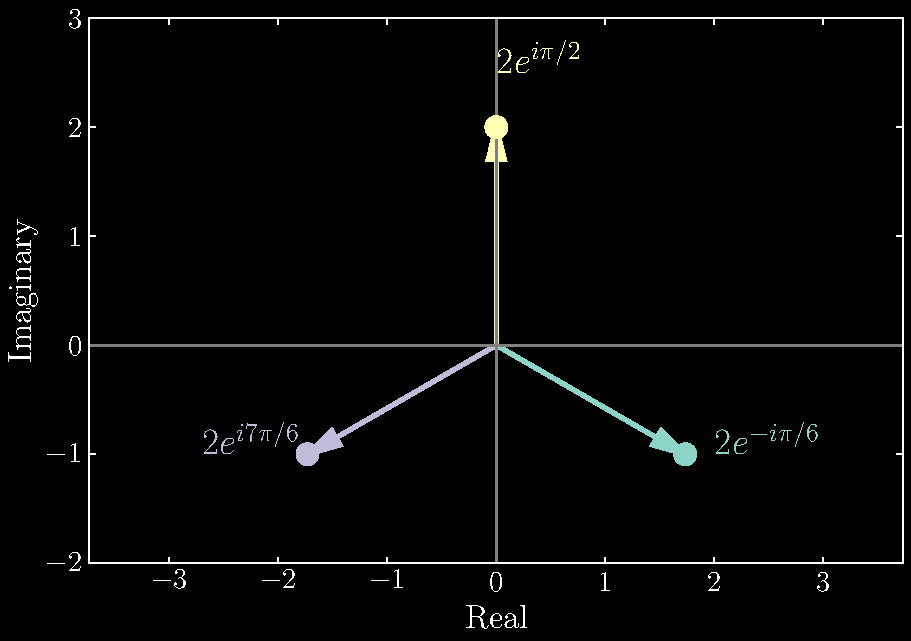
\includegraphics[width=1.0\textwidth]{../chap2/sec2.2/chap2sec2.2ex27.eps}
\end{center}

\vspace{12pt}

% QUESTION 28
\qs{2.2.28}{
\begin{enumerate}[label=(\alph*)]
	\item For which complex numbers \(s = a + i \omega \) does \(e^{st}\) approach \(0\) as \(t \rightarrow \infty\)? Those numbers \(s\) fill which ``half-plane'' in the complex plane?
	\item For which complex numbers \(s = a + i \omega \) does \(s^{n}\) approach \(0\) as \(n \rightarrow \infty\)? Those numbers \(s\) fill which part of the complex plane? Not a half-plane!
\end{enumerate}}

\begin{enumerate}[label=(\alph*)]
	\item For \(a < 0\), \(e^{st} = e^{at}e^{i \omega t}\) approaches zero.
	\item In polar form, \(s = \sqrt{a^{2} + \omega^{2}} e^{i \tan^{-1}\left( \omega / a \right)}\). We must require the modulus to be less than zero, or \(\sqrt{a^{2} + \omega^{2}} < 0\), for \(s^{n}\) to tend towards zero as \(n\) increases.
\end{enumerate}

\newpage

\subsection{\textsf{2.3 - Constant Coefficients \texorpdfstring{\(\pmb{A}\), \(\pmb{B}\), \(\pmb{C}\)}{A, B, C}}}

% QUESTION 1
\qs{2.3.1}{Substitute \(y = e^{st}\) and solve the characteristic equation for \(s\):
\begin{enumerate}[label=(\alph*)]
	\item \(2y'' + 8y' + 6y = 0\)
	\item \(y'''' - 2y'' + y = 0\)
\end{enumerate}}

\begin{enumerate}[label=(\alph*)]
	\item The characteristic equation is \(2s^{2} + 8s + 6 = 0\) which factorizes into \(2 \!\left( s + 3 \right) \!\left( s + 1 \right) = 0\). Then \(s_{1} = -3\) and \(s_{2} = -1\).
	\item The characteristic equation is \(s^{4} - 2s^{2} + 1 = 0\) which factorizes into \(\!\left( s^{2} - 1 \right)^{2} = \!\left( s - 1 \right)^{2}\!\left( s + 1 \right)^{2}\). It has repeated solutions: \(s_{1}, s_{2} = 1\) and \(s_{3}, s_{4} = -1\). 
\end{enumerate}

% QUESTION 2
\qs{2.3.2}{Substitute \(y = e^{st}\) and solve the characteristic equation for \(s = a + i \omega \):
\begin{enumerate}[label=(\alph*)]
	\item \(y'' + 2y' + 5y = 0\)
	\item \(y'''' + 2y'' + y = 0\)
\end{enumerate}}

\begin{enumerate}[label=(\alph*)]
	\item The characteristic equation is \(s^{2} + 2s + 5 = 0\), which by the quadratic formula has roots
	\[
		s_{1}, s_{2} = \frac{-2 \pm \sqrt{-16}}{2} = -1 \pm 2i
	\]
	\item The characteristic equation is \(s^{4} + 2s^{2} + 1 = 0\), which by the quadratic formula has double root
	\[
		s^{2}= \frac{-2}{2} = -1
	\]
	Rooting once more, we find repeated roots
	\[
		s_{1}, s_{2} = i, \quad s_{3}, s_{4} = -i
	\]
\end{enumerate}

% QUESTION 3
\qs{2.3.3}{Which second order equation is solved by \(y = c_{1}e^{-2t} + c_{2}e^{-4t}\)? Or \(y = te^{5t}\)?}

In the first instance, the roots are \(s_{1} = -2\) and \(s_{2} = -4\). Then the characteristic polynomial is \(\!\left( s + 2 \right) \!\left( s + 4 \right) = s^{2} + 6s + 8\), corresponding to second order equation \(y'' + 6y' + 8y = 0\). In the second case, we have repeated roots \(s_{1}, s_{2} = 5\), which has characteristic polynomial \(\!\left( s - 5 \right)^{2} = s^{2} - 10s + 25\). This corresponds to second order equation \(y'' - 10y' + 25y = 0\).

\vspace{12pt}

% QUESTION 4
\qs{2.3.4}{Which second order equation has solutions \(y = c_{1}e^{-2t} \cos\left( 3t \right) + c_{2}e^{-2t}\sin\left( 3t \right)\)?}

The complex roots are \(s_{1} = -2 + 3i\) and \(s_{2} = -2 - 3i\), with characteristic polynomial \(s^{2} - 4s + 13\). This corresponds to second order equation 
\[
	y'' - 4y' + 13 = 0
\]

% QUESTION 5
\qs{2.3.5}{Which numbers \(B\) give (under)(critical)(over) damping in \(4y'' + By' + 16y = 0\)?}

\textbf{Underdamping}: We must have \(B^{2} < 4AC\), or in this case, \(B^{2} < 256\). Then we must have \(\abs{B} < 16\).

\textbf{Critical damping}: We have \(B^{2} = 4AC\), or \(B^{2} = 256\), implying \(\abs{B} = 16\).

\textbf{Overdamping}: We have \(B^{2} > 4AC\), or \(B^{2} > 256\), implying \(\abs{B} > 16\).

\vspace{12pt}

% QUESTION 6
\qs{2.3.6}{If you want oscillation from \(my'' + by' + ky = 0\), then \(b\) must stay below \underline{\qquad}.}

We must have \(b^{2} < 4mk\) or \(\abs{b} < 2 \sqrt{mk}\).

\vspace{12pt}

% QUESTION 7
\qs{2.3.7}{The roots \(s_{1}\) and \(s_{2}\) satisfy \(s_{1} + s_{2} = -2p = -B/A\) and \(s_{1}s_{2} = p^{2} + \omega^{2}_{n} = C/A\). Show this two ways:

\begin{enumerate}[label=(\alph*)]
	\item Start from \(A^{2} + Bs + C = A \!\left( s - s_{1} \right) \!\left( s - s_{2} \right) \). Multiply to see \(s_{1}s_{2}\) and \(s_{1} + s_{2}\).
	\item Start from \(s_{1} = -p + i \omega_{d}\), \(s_{2} = -p - i \omega_{d}\)
\end{enumerate}}

\begin{enumerate}[label=(\alph*)]
	\item We write
	\begin{align*}
		A^{2} + Bs + C & = A \!\left( s - s_{1} \right) \!\left( s - s_{2} \right)  \\
		 & = A \!\left( s^{2} - s \!\left( s_{1} + s_{2} \right) + s_{1}s_{2} \right)  
	\end{align*}
	Concluding that \(B = -A\!\left( s_{1} + s_{2} \right) \) and \(C = As_{1}s_{2}\). Then
	\[
		-\frac{B}{A} = s_{1} + s_{2}, \quad \frac{C}{A} = s_{1}s_{2}
	\]
	\item Let \(s_{1} = -p + i \omega_{d}\) and \(s_{2} = -p - i \omega_{d}\). Then \(s_{1} + s_{2} = -2p\) and
	\[
		s_{1}s_{2} = \!\left( -p + i \omega_{d} \right) \!\left( -p - i \omega_{d} \right) = p^{2} + \omega^{2}_{d}
	\]
\end{enumerate}
\textbf{Note}: There are two errors in the problem statement. The textbook erroneously has the equalities \(s_{1} + s_{2} = -B/2A\) and \(s_{1}s_{2} = p^{2} + \omega^{2}_{n}\). The corrections have been made in my writing of the problem above.

\vspace{12pt}

% QUESTION 8
\qs{2.3.8}{Find \(s\) and \(y\) at the bottom point of the graph of \(y = As^{2} + Bs + C\). At that minimum point \(s = s_{\text{min}}\) and \(y = y_{\text{min}}\), the slope is \(dy/ds = 0\).}

Differentiate with respect to \(s\) to find
\[
	\frac{d y}{d s} = 2As + B = 0 \quad \implies \quad s_{\text{min}} = -\frac{B}{2A}
\]
The corresponding \(y_{\text{min}}\) is
\begin{align*}
	y_{\text{min}} & = A \!\left( - \frac{B}{2A} \right)^{2} + B \!\left( -\frac{B}{2A} \right) + C \\
		   & = \frac{B^{2}}{4A} - \frac{B^{2}}{2A} + C \\
		   & = -\frac{B^{2}}{4A} + C
\end{align*}

% QUESTION 9
\qs{2.3.9}{The parabolas in Figure 2.10 show how the graph of \(y = As^{2} + Bs + C\) is raised by increasing \(B\). Using Problem 8, show that the bottom point of the graph moves left (change in \(s_{\text{min}}\)) and down (change in \(y_{\text{min}}\)) when \(B\) is increased by \(\Delta B\).}

Assume \(\Delta B > 0\). By Problem 8, the new \(s_{\text{min}}\) becomes
\[
	s_{\text{min}} = -\frac{\!\left( B + \Delta B \right) }{2A} < -\frac{B}{2A}
\]
and the new \(y_{\text{min}}\)
\[
	y_{\text{min}} = -\frac{\!\left( B + \Delta B \right)^{2}}{4A} + C = -\frac{\!\left( B^{2} + 2B \Delta B + \Delta B^{2} \right) }{4A} + C < -\frac{B^{2}}{4A} + C
\]
both of which correspond to a leftward and downward shift, respectively.

\vspace{12pt}

\newpage
% QUESTION 10
\qs{2.3.10}{(recommended) Draw a picture to show the paths of \(s_{1}\) and \(s_{2}\) when \(s^{2} + Bs + 1 = 0\) and the damping increases from \(B = 0\) to \(B = \infty\). At \(B = 0\), the roots are on the \underline{\quad} axis. As \(B\) increases, the roots travel on a circle (why?). At \(B = 2\), the roots meet on the real axis. For \(B > 2\) the roots separate to approach \(0\) and \(-\infty\). \textit{Why is their product \(s_{1}s_{2}\) always equal to \(1\)}?}

The roots are
\[
	s = \frac{-B \pm \sqrt{B^{2} - 4}}{2}
\]
When \(B = 0\), the roots are \(s_{1,2} = \pm i\), which lie on the imaginary axis. The roots travel on a circle as \( B  \) grows because they are complex conjugates, and given that the modulus of the roots remains constant, a quarter-circle traced out by the complex vector for one root will be reflected over the real axis for the other root, conforming to the geometry of a circle.

\begin{center}
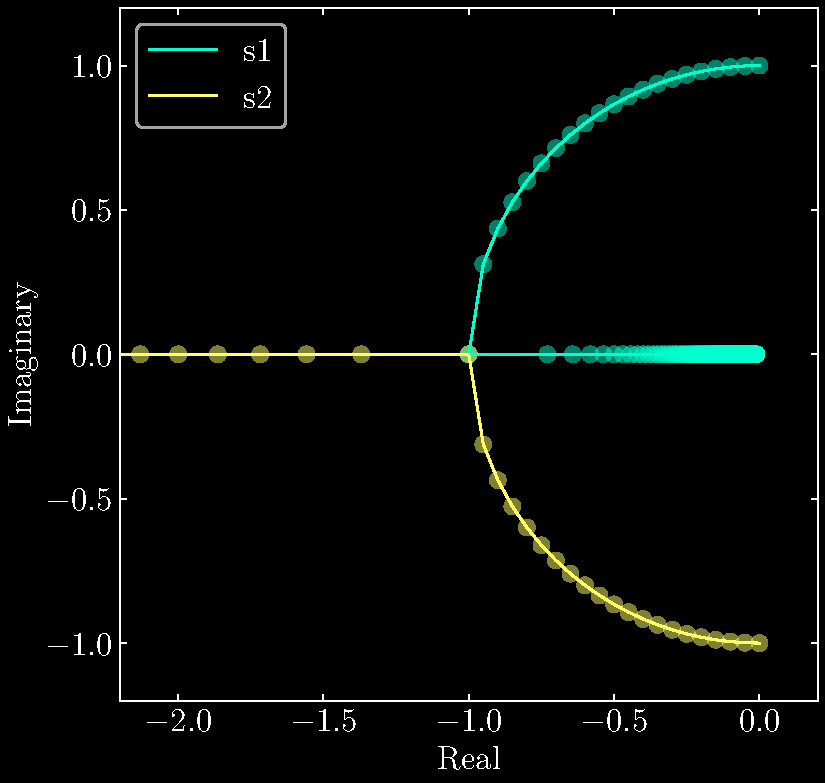
\includegraphics[width=1.0\textwidth]{../chap2/sec2.3/chap2sec2.3ex10.pdf}
\end{center}

Recall from problem 7 that \(s_{1}s_{2} = C / A = 1\). Another, more intuitive approach is to realize that, \( s_{1} = \overline{s_{2}} \), so they are complex conjugates of one another, and their product is the modulus (in this case, unity).

% QUESTION 11
\qs{2.3.11}{(this too if possible) Draw the paths of \( s_{1} \) and \( s_{2} \) when \( s^{2} + 2s + k = 0\) and the stiffness increases from \( k = 0 \) to \( k = \infty \). When \( k = 0 \), the roots are \underline{\quad}. At \( k = 1 \), the roots meet at \( s =  \) \underline{\qquad}. For \( k \rightarrow \infty \) the two roots travel up/down on a \underline{\qquad} in the complex plane. \textit{Why is their sum \( s_{1} + s_{2} \) always equal to \( -2 \)}?}

The roots are
\[
	s = \frac{-2 \pm \sqrt{2^{2} - 4k}}{2} = -1 \pm \sqrt{1 - k}
\]
When \( k = 0 \), the roots are \( s_{1,2} = 0, -2 \). Once we reach \( k = 1 \), we have double roots with \( s_{1,2} = -1 \). As \( k \) increases to infinity, the real component remains fixed, while the imaginary component grows in both directions on the vertical axis. Altogether, the trajectory of the roots forms a cross.

\begin{center}
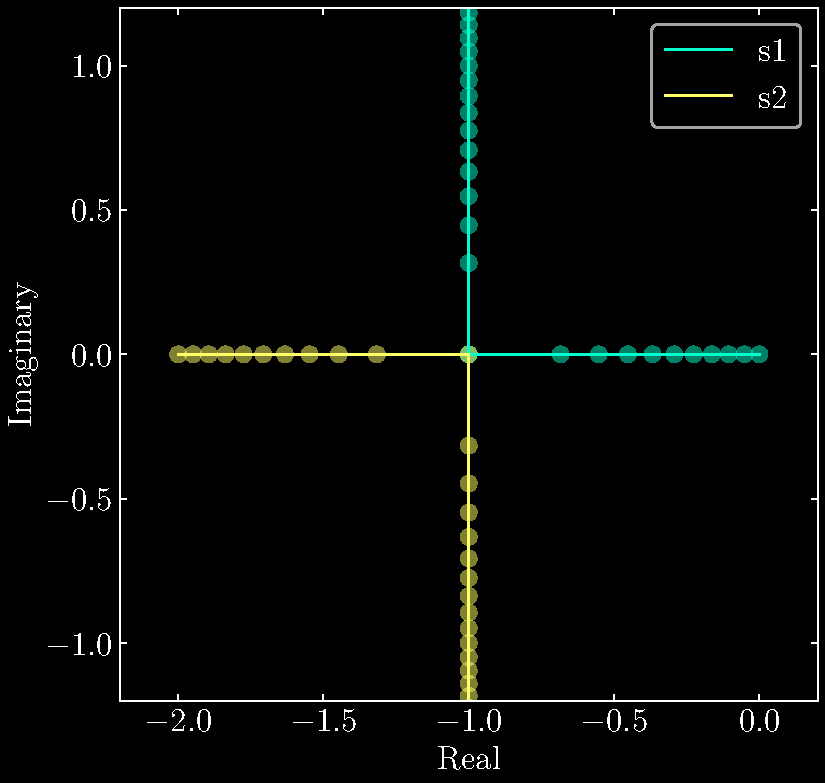
\includegraphics[width=1.0\textwidth]{../chap2/sec2.3/chap2sec2.3ex11.pdf}
\end{center}

As for their sum, observe that the imaginary components of \( s_{1,2} \) cancel, and the real parts add to \( -2 \).

\vspace{12pt}

% QUESTION 12
\qs{2.3.12}{If a polynomial \( P \!\left( s  \right) \) has a double root at \( s = s_{1} \), then \( \!\left( s - s_{1} \right) \) is a double factor and \( P \!\left( s  \right) = \!\left( s - s_{1} \right)^{2} Q \!\left( s  \right) \). Certainly \( P = 0 \) at \( s = s_{1} \). Show that also \( dP/ds = 0 \) at \( s = s_{1} \). use the product rule to find \( dP/ds  \).}

By the product rule, we have
\[
	\frac{d P }{d s }_{\!\left( s = 0 \right)} = 2 \!\left( s - s_{1} \right) Q \!\left( s  \right) + \!\left( s - s_{1} \right)^{2} \frac{d Q }{d s } = 0
\]

% QUESTION 13
\qs{2.3.13}{Show that \( y'' = 2ay' - \!\left( a^{2} + \omega^{2} \right)y \) leads to \( s = a \pm i \omega \). Solve \( y'' - 2y' + 10y = 0 \).}

The characteristic equation is given by
\[
	s^{2} - 2as + \!\left( \alpha^{2} + \omega^{2} \right) = 0 
\]
which has roots
\[
	s = \frac{2a \pm \sqrt{4a^{2} - 4 \!\left( \alpha^{2} + \omega^{2} \right)}}{2} = a \pm i \omega 
\]
For the given equation, we have \( a = 1 \) and \( \omega = 3 \). Then we have solution
\begin{alignat*}{1}
y \!\left( t  \right) & = e^{\!\left( 1 + 3i \right)t} + e^{\!\left( 1 - 3i \right)t} \\
	 & = 2e^{t} \cos\!\left( 3t \right)  \\ 
\end{alignat*}

% QUESTION 14
\qs{2.3.14}{The undamped \textit{natural frequency} is \( \omega_{n } = \sqrt{k / m } \). The two roots of \( ms^{2} + k = 0 \) are \( s = \pm i \omega_{n } \) (pure imaginary). With \( p = b / 2m \), the roots of \( ms^{2} + bs + k = 0 \) are \( \pmb{s_{1}, s_{2} = -p \pm \sqrt{p^{2} - \omega^{2}_{n }}} \). The coefficient \( p = b / 2m  \) has the units of 1 / time.

Solve \( s^{2} + 0.1s + 1 = 0 \) and \( s^{2} + 10s + 1 = 0 \) with numbers correct to two decimals.}

In the first equation, we have \( m = 1 \), \( b = 0.1 \), and \( k = 1 \). Then \( p = 0.05 \) and \( \omega_{n } = 1 \). This yields roots \( s_{1,2} = -0.05 \pm 0.99i \).

The second equation gives us \( p = 5 \) and \( \omega_{n } = 1 \), which has roots \( s_{1,2} = -5 \pm \sqrt{24} = -0.10, -9.89 \).

\vspace{12pt}

% QUESTION 15
\qs{2.3.15}{With large overdamping \( \pmb{p >> \omega_{n }} \), the square root \( \sqrt{p^{2} - \omega^{2}_{n }} \) is close to \( p - \omega^{2}_{n } / 2p \). Show that the roots of \( ms^{2} + bs + k \) are \( s_{1} \approx \pmb{-\omega^{2}_{n } / 2p} =\) (small) and \( s_{2} \approx -2p = \pmb{-b/m } \) (large).}

From question 14, the roots are \( s_{1}, s_{2} = -p \pm \sqrt{p^{2} - \omega^{2}_{n}} \). By the overdamping assumption, the roots can then be approximated by \( s_{1} \approx -\omega^{2}_{n } / 2p \) and \( s_{2} \approx -2p - \omega^{2}_{n } / 2p \approx -2p = -b / m  \), appealing to the fact that \( p >> \omega_{n } \).

\vspace{12pt}

% QUESTION 16
\qs{2.3.16}{With small underdamping \( \pmb{p << \omega_{n }} \), the square root of \( p^{2} - \omega^{2}_{n } \) is approximately \( i \omega_{n } - ip^{2} / 2 \omega_{n } \). Square that to come close to \( p^{2} - \omega^{2}_{n } \). Then the frequency for small underdamping is reduced to \( \omega_{d } \approx \omega_{n } - p^{2} / 2 \omega_{n } \).}

Write
\[
	\!\left( i \omega_{n } - i p^{2} / 2 \omega_{n } \right)^{2} = p^{2} - \omega^{2}_{n } + \frac{p^{4}}{4 \omega^{2}_{n }} \approx p^{2} - \omega^{2}_{n }
\]
Since we have underdamping, the magnitude of the square root of \( p^{2} - \omega^{2}_{n } \) is approximated as \( \omega_{d } \approx \omega_{n } - p^{2} / 2 \omega_{n } \).

\vspace{12pt}

% QUESTION 17
\qs{2.3.17}{Here is an 8th order equation with eight choices for solutions \( y = e^{st } \):
\[
	\frac{d^{8}y }{dt^{8}} = y \quad \text{becomes} \quad s^{8}e^{st } = e^{st } \quad \text{and} \quad \pmb{s^{8} = 1} : 
\]
\[
	\text{Eight roots in Figure 2.6} 
\]
Find two solutions \( e^{st } \) that don't oscillate ( \( s  \) is real). Find two solutions that only oscillate ( \( s  \) is imaginary). Find two that spiral into zero and two that spiral out.}

The eighth roots of unity are:
\[
	1, -1, i, -i, e^{i \pi / 4}, e^{i 3 \pi / 4}, e^{i 5 \pi / 4}, e^{i 7 \pi / 4} 
\]
The real solutions are \( e^{t } \) and \( e^{-t } \) and imaginary are \( e^{it } \) and \( e^{-it } \). In order for the solutions to spiral into zero, the real component of \( s  \) must be negative, ensuring that the outer exponential decays with increasing \( t  \). This corresponds to the solutions involving \( e^{i 3 \pi / 4} \) and \( e^{i 5 \pi / 4} \):
\begin{align*}
	& e^{t \cos\!\left( 3 \pi / 4 \right)} \!\left[ \cos\!\left( t \sin\!\left( \frac{3 \pi }{4} \right) \right) + \sin\!\left( t \sin\!\left( \frac{3 \pi }{4} \right) \right) \right] \\[12pt]
	& e^{t \cos\!\left( 5 \pi / 4 \right)} \!\left[ \cos\!\left( t \sin\!\left( \frac{5 \pi }{4} \right) \right) + \sin\!\left( t \sin\!\left( \frac{5 \pi }{4} \right) \right) \right] 
\end{align*}
Lastly, the solutions that spiral away from zero involve \( e^{i \pi / 4} \) and \( e^{i 7 \pi / 4} \), and they are
\begin{align*}
	& e^{t \cos\!\left( \pi / 4 \right)} \!\left[ \cos\!\left( t \sin\!\left( \frac{\pi }{4} \right) \right) + \sin\!\left( t \sin\!\left( \frac{\pi }{4} \right) \right) \right] \\[12pt]
	& e^{t \cos\!\left( 7 \pi / 4 \right)} \!\left[ \cos\!\left( t \sin\!\left( \frac{7 \pi }{4} \right) \right) + \sin\!\left( t \sin\!\left( \frac{7 \pi }{4} \right) \right) \right] 
\end{align*}
Observe here that the outer exponentials have positive arguments, ensuring growth as \( t  \) grows.

\vspace{12pt}

% QUESTION 18
\qs{2.3.18}{
\[
	A_{n } \frac{d^{n }y}{dt^{n }} + \cdots + A_{1}\frac{d y}{d t } + A_{0}y = 0 \text{ leads to } \pmb{A_{n }s^{n } + \cdots + A_{1}s + A_{0} = 0.} 
\]
The \( n  \) roots \( s_{1}, ..., s_{n } \) produce \( n  \) solutions \( y \!\left( t  \right) = e^{st }\) (if those roots are distinct). Write down \( n  \) equations for the constants \( c_{1} \) to \( c_{n } \) in \( y = c_{1}e^{s_{1}t } + \cdots + c_{n }e^{s_{n }t } \) by matching the \( n  \) initial conditions for \( y \!\left( 0 \right) \), \( y'\!\left( 0 \right) \), ..., \( D^{n - 1}y \!\left( 0 \right) \).}

Matching the initial conditions, we write
\begin{alignat*}{1}
	 y \!\left( 0 \right) & = c_{1} + \cdots c_{n }  \\
	 y'\!\left( 0 \right) & = c_{1}s_{1} + \cdots + c_{n }s_{n } \\ 
			      & \quad \vdots \\
	 D^{n - 1}y \!\left( 0 \right) & = c_{1}s^{n - 1}_{1} + \cdots + c_{n }s^{n - 1}_{n}
\end{alignat*}

% QUESTION 19
\qs{2.3.19}{\textbf{Find two solutions to } \( \pmb{d^{2015}y / dt^{2015} = dy/dt } \). Describe all solutions to \( s^{2015} = s  \).}

Two solutions are \( y = e^{t } \) and \( y = e^{-t } \). The set of all solutions to \( s^{2015} = s \) is described by 0 and 
\[
	e^{i 2 k \pi / 2014} \text{ for } k \in \!\left\{ 0, ..., 2013 \right\}
\]

% QUESTION 20
\qs{2.3.20}{The solution to \( y'' = 1 \) starting from \( y \!\left( 0 \right) = y'\!\left( 0 \right) = 0 \) is \( y \!\left( t  \right) = t^{2} / 2 \). The fundamental solution to \( g'' = \delta \!\left( t  \right) \) is \( g \!\left( t  \right) = t  \) by Example 5. Does the integral \( \int g \!\left( t - s  \right) f \!\left( s  \right) ds = \int \!\left( t - s  \right) ds  \) from 0 to \( t  \) give the correct solution \( y = t^{2} / 2 \)?}

The forcing function \( f \!\left( t  \right) \) here simply equals 1, hence the particular solution reduces to solving
\[
	\int_{0}^{t } \!\left( t - s  \right) \, ds = -\frac{\!\left( t - s  \right)^{2}}{2} \Big|^{t }_{0} = \frac{t^{2}}{2}
\]

\newpage

% QUESTION 21
\qs{2.3.21}{The solution to \( y'' + y = 1 \) starting from \( y \!\left( 0 \right) = y'\!\left( 0 \right) = 0 \) is \( y = 1 - \cos t  \). The solution to \( g'' + g = \delta \!\left( t  \right) \) is \( \pmb{g \!\left( t  \right) = \sin t } \) by equation (13) with \( \omega = 1 \) and \( A = 1 \). Show that \( 1 - \cos t  \) agrees with the integral \( \int g \!\left( t - s  \right) f \!\left( s  \right)ds = \int \sin\!\left( t - s \right)ds \).}

We have
\[
	\int_{0 }^{t} \sin\!\left( t - s  \right) \, ds = \cos\!\left( t - s \right) \Big|^{t }_{0} = 1 - \sin\!\left( t \right)
\]

% QUESTION 22
\qs{2.3.22}{The step function \( H \!\left( t  \right) = 1\) for \( t \ge 0 \) is the integral of the delta function. \textbf{So the step response } \( \pmb{r \!\left( t  \right)} \) \textbf{is the integral of the impulse response.} This fact must also come from our basic solution formula:
\[
	Ar'' + Br' + Cr = 1 \text{ with } r \!\left( 0 \right) = r'\!\left( 0 \right) = 0 \text{ has } \pmb{r \!\left( t  \right) = \int_{0}^{t } g \!\left( t - s  \right) \, ds  } 
\]
Change \( t - s  \) to \( \tau  \) and change \( ds  \) to \( -d \tau  \) to confirm that \( r \!\left( t  \right) = \int_{0}^{t } g \!\left( \tau \right) \, d \tau   \).

Section 2.5 will find two good formulas for the step response \( r \!\left( t  \right) \).}

Let \( \tau = t - s  \). Then \( d \tau / ds = -1 \), implying \( ds = -d \tau  \). Lastly, the change of variables implies the change of integration bounds: \( s_{\text{upper}} = t  \) goes to \( \tau_{\text{upper}} = t - t = 0 \) and \( s_{\text{lower}} = 0 \) goes to \( \tau_{\text{lower}} = t - 0 = t  \). Thus we have
\[
	r \!\left( t  \right) = -\int_{t }^{0} g \!\left( \tau  \right) \, d \tau = \int_{0}^{t } g \!\left( \tau  \right) \, d \tau   
\]

\newpage
\subsection{\textsf{2.4 - Forced Oscillations and Exponential Response}}

\textbf{Problems 1-4 use the exponential response } \( \pmb{y_{p } = e^{ct } / P \!\left( c  \right)} \) \textbf{ to solve } \( \pmb{P \!\left( D  \right) y = e^{ct }} \).

\vspace{12pt}

% QUESTION 1
\qs{2.4.1}{Solve these constant coefficient equations with exponential driving force:
\begin{enumerate}[label=(\alph*)]
	\item \( y''_{p } + 3y'_{p } + 5y_{p } = e^{t } \)
	\item \( 2y''_{p } + 4y_{p } = e^{it } \)
	\item \( y'''' = e^{t } \)
\end{enumerate}}

\begin{enumerate}[label=(\alph*)]
	\item Let \( y_{p } = Y e^{t } \). Without using \( P \!\left( D  \right) y = e^{ct } \), we have
	\begin{alignat*}{2}
		 && Ye^{t } + 3Ye^{t } + 5Ye^{t } & = e^{t } \\
		 \implies && 9Y & = 1 \\ 
		 \implies && Y & = 1 / 9
	\end{alignat*}
	Thus \( \displaystyle{y_{p } = \frac{1}{9} e^{t }} \). Note that \( P \!\left( 1 \right) = 1^{2} + 3 \cdot 1 + 5 = 9 \).
	\item Using \( P \!\left( D  \right)y = e^{ct} \), we have
	\[
		y_{p } = \frac{e^{it }}{P \!\left( i  \right)} = \frac{e^{it }}{-2 + 4} = \frac{e^{it }}{2}
	\]
	\item Using \( P \!\left( D  \right)y = e^{ct } \), we have
	\[
		y_{p } = \frac{e^{t }}{P \!\left( 1  \right)} = e^{t}
	\]
\end{enumerate}

% QUESTION 2
\qs{2.4.2}{These equations \( P \!\left( D  \right)y = e^{ct } \) use the symbol \( D  \) for \( d / dt  \). Solve for \( y_{p }\!\left( t  \right) \):
\begin{enumerate}[label=(\alph*)]
	\item \( \!\left( D^{2} + 1 \right)y_{p }\!\left( t  \right) = 10e^{-3t } \)
	\item \( \!\left( D^{2} + 2D + 1 \right)y_{p }\!\left( t  \right) = e^{i \omega t } \)
	\item \( \!\left( D^{4} + D^{2} + 1 \right)y_{p } \!\left( t  \right) = e^{i \omega t} \)
\end{enumerate}}

\begin{enumerate}[label=(\alph*)]
	\item \( \displaystyle{y_{p } \!\left( t  \right) = \frac{10}{\!\left( -3 \right)^{2} + 1} e^{-3t } = e^{-3t}} \)
	\item \( \displaystyle{y_{p } \!\left( t  \right) = \frac{1}{-\omega^{2} + 2\omega i + 1}e^{i \omega t } = \frac{1}{1 - \omega^{2} + 2 \omega i } e^{i \omega t} } \)
	\item \( \displaystyle{y_{p }\!\left( t  \right) = \frac{1}{1 - \omega^{2} + \omega^{4}} e^{i \omega t }} \)
\end{enumerate}

% QUESTION 3
\qs{2.4.3}{How could \( y_{p } = e^{ct } / P \!\left( c  \right) \) solve \( y'' + y = e^{t }e^{it } \) and then \( y'' + y = e^{t } \cos t \)?}

Observe that \( y_{p } \) solves the first equation when \( c = \!\left( 1 + i  \right)t  \), and then the real part serves as the solution to the second.
\begin{align*}
	y_{p } = \frac{e^{\!\left( 1 + i  \right)t }}{P \!\left( 1 + i  \right)} = \frac{1}{1 + 2i}e^{t }e^{it} & = \frac{1 - 2i}{5}e^{t } \!\left[ \cos\!\left( t \right) + i \sin\!\left( t \right) \right] \\
														& = \underbrace{\frac{1}{5}e^{t }\!\left[ \cos\!\left( t  \right) + 2\sin\!\left( t \right) \right]}_{\text{Solution to second equation}} + \frac{i}{5} e^{t } \!\left[ -2 \cos\!\left( t \right) + \sin\!\left( t \right)\right]
\end{align*}

% QUESTION 4
\qs{2.4.4}{\begin{enumerate}[label=(\alph*)]
	\item What are the roots \( s_{1} \) to \( s_{3} \) and the null solutions to \( y_{n }''' - y_{n } = 0 \)?
	\item Find particular solutions to \( y_{p }''' - y_{p } = e^{it } \) and to \( y_{p }''' - y_{p } = e^{t } - e^{i \omega t } \).
\end{enumerate}}

\begin{enumerate}[label=(\alph*)]
	\item The roots are \( s_{1} = 1 \), \( s_{2} = e^{i 2 \pi / 3} = \cos\!\left(2 \pi / 3\right) + i \sin\!\left(2 \pi / 3\right)  \), and \( s_{3} = e^{i 4 \pi / 3} = \cos\!\left(4 \pi / 3 \right) + i \sin\!\left(4 \pi / 3 \right) \). The null solution is
	\begin{align*}
		y_{n } & = c_{1}e^{t} + c_{2}e^{\!\left( -1/2 + i \sqrt{3}/2 \right)t } + c_{3}e^{\!\left( -1/2 - i \sqrt{3}/2 \right)t } \\
		       & = c_{1}e^{t } + \!\left( c_{2} + c_{3} \right)e^{-t/2}\cos\!\left( \frac{\sqrt{3}}{2}t \right) + i \!\left( c_{2} - c_{3} \right)e^{-t/2}\sin\!\left( \frac{\sqrt{3}}{2}t \right)
        \end{align*}	
\item For the first equation, we have \( \displaystyle{y_{p} = \frac{1}{-1-i}}e^{it} \). In the second case, appeal to the superposition principle to separately calculate the particular solution for each forcing term to find
	\[
		y_{p } = \frac{te^{t }}{3} + \frac{1}{1 + i \omega^{3}} e^{i \omega t} 
	\]
	Decomposed into real and imaginary components, we can rewrite as:
	\[
		y_{p } = \frac{te^{t }}{3} + \frac{\cos\!\left(\omega t \right) + \omega^{3} \sin\!\left(\omega t \right) }{1 + \omega^{6}} + i \!\left[ \frac{\sin\!\left(\omega t \right)  - \omega^{3} \cos\!\left(\omega t \right) }{1 + \omega^{6}} \right] 
	\]
\end{enumerate}

% QUESTION 5
\qs{2.4.5}{Which value of \( C  \) gives resonance in \( y'' + Cy = e^{i \omega t } \)? Why do we never get resonance in \( y'' + 5y' + Cy = e^{i \omega t } \)?}

We must have \( P \!\left( i \omega  \right) = \!\left( i \omega \right)^{2} + C = 0\) for some value of \( C  \). It immediately follows that we must have \( C = \omega^{2} \). In the second case, observe that the roots of \( P \!\left( s  \right) = s^{2} + 5s + C  \) can never be pure imaginary. Thus it is impossible for \( s = i \omega \) to ever be a solution to \( P \!\left( s  \right) = 0 \).

% QUESTION 6
\qs{2.4.6}{Suppose the third order equation \( P \!\left( D  \right) y_{n } = 0 \) has solutions \( y = c_{1}e^{t } + c_{2}e^{2t } + c_{3}e^{3t } \). What are the null solutions to the sixth order equation \( P \!\left( D  \right) P \!\left( D  \right)y_{n } = 0 \)?}

We must have repeated roots, as we can think of \( P \!\left( D  \right) \) as repeated `factors` to the polynomial corresponding to the sixth order equation. With repeated roots, we must have
\[
	y = c_{1}e^{t} + c_{2}e^{2t} + c_{3}e^{3t} + c_{4}te^{t} + c_{5}te^{2t} + c_{6}te^{3t} 
\]

% QUESTION 7
\qs{2.4.7}{Complete this table with equations for \( s_{1} \) and \( s_{2} \) and \( y_{n } \) and \( y_{p } \):
\begin{alignat*}{3}
	& \textbf{Undamped free oscillation} && \quad my'' + ky = 0 && \quad \pmb{y_{n }} = \underline{\qquad} \\
	& \textbf{Undamped forced oscillation} && \quad my'' + ky = e^{i \omega t } && \quad \pmb{y_{p }} = \underline{\qquad} \\
	& \textbf{Damped free motion} && \quad my'' + by' + ky = 0 && \quad \pmb{y_{n }} = \underline{\qquad} \\
	& \textbf{Damped forced motion} && \quad my'' + by' + ky = e^{ct } && \quad \pmb{y_{p }} = \underline{\qquad}
\end{alignat*}}

Let \( \omega_{n } = \sqrt{k / m } \). In the order of the table:
\begin{enumerate}[label=(\alph*)]
	\item Solve \( s^{2} + \omega_{n}^{2} = 0 \) to find
	\[ 
		s_{1,2} = \pm i \omega_{n}, \quad \displaystyle{ y_{n } = c_{1} \cos\!\left( \omega_{n } t \right) + ic_{2}\sin\!\left( \omega_{n } t \right) } 
	\]
	\item Divide through by \( m  \) and \( P \!\left( i \omega  \right) = \!\left( i \omega  \right)^{2} + \omega_{n} = \omega_{n} - \omega^{2} \). Then we have
	\[
		y_{p } = \frac{1}{m \!\left( \omega_{n}^{2} - \omega^{2} \right)}e^{i \omega t}
	\]
	\item Solve \( s^{2} + \!\left( b / m  \right)s + \omega_{n}^{2} = 0 \) to find
	\[
		s = \frac{-b/m \pm \sqrt{\displaystyle{\frac{b^{2} }{m^{2}}} - 4 \omega^{2}_{n} }}{2} = \frac{-b \pm \sqrt{b^{2} - 4mk}}{2m}
	\]
	This leads us to null solution
	\[
		y_{n} = e^{-b / 2m} \!\left( c_{1} e^{\!\left( \sqrt{b^{2} - 4mk} \right) t} + c_{2} e^{-\!\left( \sqrt{b^{2} - 4mk} \right) t} \right) 
	\]
	\item Divide through by \( m  \) and \( P \!\left( c  \right) = c^{2} + \!\left( b/m  \right)c + k / m \). Then we have
	\[
		y_{p } = \frac{1}{mc^{2} + bc + k} e^{ct}
	\]
\end{enumerate}

% QUESTION 8
\qs{2.4.8}{Complete the same table when the coefficients are 1 and \( 2 Z_{\omega_{n }} \) and \( \omega^{2}_{n } \) with \( Z < 1 \).
\begin{alignat*}{3}
	& \textbf{Undamped and free} && \quad y'' + \omega^{2}_{n }y = 0 && \quad \pmb{y_{n }} = \underline{\qquad} \\
	& \textbf{Undamped and forced} && \quad y'' + \omega^{2}_{n } y = e^{i \omega t } && \quad \pmb{y_{p }} = \underline{\qquad} \\ 
	& \textbf{Underdamped and free} && \quad y'' + 2Z \omega_{n } y' + \omega^{2}_{n } y = 0 && \quad \pmb{y_{n}} = \underline{\qquad} \\
	& \textbf{Underdamped and forced} && \quad y'' + 2Z \omega_{n } y' + \omega^{2}_{n } y = e^{ct } && \quad \pmb{y_{p }} = \underline{\qquad}
\end{alignat*}
}

Let \( Z = b / \sqrt{4mk} \) and \( \omega_{n } \) be as before. These are similar equations as in the previous question, but using different variable definitions.

\begin{enumerate}[label=(\alph*)]
	\item Solve \( s^{2} + \omega^{2}_{n } = 0 \) to find roots \( s = \pm i \omega_{n } \). The null solution is
	\[
		y_{n } = c_{1} e^{i \omega_{n } t } + c_{2} e^{-i \omega_{n } t} = C_{1} \cos\!\left( \omega_{n } t \right) + i C_{2} \sin\!\left( \omega_{n } t \right)  
	\]
	\item Calculate \( P \!\left( i \omega \right) = \omega^{2} + \omega^{2}_{n } \) and divide the right-hand side by \( P \!\left( i \omega \right) \)to find
	\[
		y_{p } = \frac{1}{\omega^{2} + \omega^{2}_{n }} e^{i \omega t} 
	\]
	\item Solve \( s^{2} + 2Z \omega_{n } s + \omega^{2}_{n } = 0 \) to find roots
	\[
		s = \frac{-2Z \omega_{n } \pm \sqrt{4 Z^{2} \omega^{2}_{n } - 4 \omega^{2}_{n }}}{2} = -Z \omega_{n } \pm i \omega_{n } \sqrt{1 - Z^{2}}
	\]
	with the imaginary term ensuing from the premise that \( Z < 1 \). This leads us to the null solution
	\[
		y_{n } = e^{-Z \omega_{n}} \!\left[ c_{1} \cos\!\left( \omega_{n } \!\left( \sqrt{1 - Z^{2}} \right) t \right) + ic_{2} \sin\!\left( \omega_{n } \!\left( \sqrt{1 - Z^{2}} \right) t \right)  \right] 
	\]
	\item Calculate \( P \!\left( c  \right) = c^{2} + 2 Z \omega_{n } c + \omega^{2}_{n } \) and divide the right-hand side by \( P \!\left( c  \right) \) to get
	\[
		y_{p } = \frac{1}{c^{2} + 2 Z \omega_{n } c + \omega^{2}_{n }} e^{ct} 
	\]
\end{enumerate}

% QUESTION 9
\qs{2.4.9}{What equations \( y'' + By' + Cy = f  \) have these solutions?
\begin{enumerate}[label=(\alph*)]
	\item \( y = c_{1} \cos\!\left( 2t \right) + c_{2} \sin\!\left( 2t \right) + \cos\!\left( 3t \right) \)
	\item \( y = c_{1}e^{-t } \cos\!\left( 4t \right) + c_{2} e^{-t } \sin\!\left( 4t \right) + \cos\!\left( 5t \right)  \)
	\item \( y = c_{1} e^{-t } + c_{2} t e^{-t } + e^{i \omega t}  \)
\end{enumerate}}

\begin{enumerate}[label=(\alph*)]
	\item The first two terms constitute the null solution. One solution is to substitute the null solution in the equation, and deducing that in collecting the sine and cosine terms, \( B  \) and \( C  \) must be such that these equations vanish:
	\begin{align*}
		-4 c_{1} + 2B c_{2} + Cc_{1} & = 0 \\
		-4 c_{2} - 2B c_{1} + Cc_{2} & = 0 
	\end{align*}
	We can conclude that \( B = 0 \) and \( C = 4 \). 

	Alternatively, recall from question 2.3.7 that \( s_{1} + s_{2} = B/A \) and \( s_{1}s_{2} = C/A  \) (we call these Vieta's formulas, which can be generalized to any polynomial of degree \( n  \)). From the absence of the damping term, we can surmise that the null solution is undamped and freely oscillates, with roots \( s_{1,2} = \pm 2i \). Using Vieta's formulas, we have \( s_{1} + s_{2} = B = 0 \) and \( s_{1}s_{2} = C = 4 \).

	The homogeneous equation is
	\[
		y'' + 4y = 0
	\]
	For the forcing term \( f \), substitute the particular solution to derive
	\[
		 -9 \cos\!\left( 3t \right) + 4 \cos\!\left( 3t \right) = f = -5 \cos\!\left( 3t \right) 
	\]
	\item The roots are \( s_{1,2} = -1 \pm 4i \), which lead to polynomial \( s^{2} + 2s + 17 \). Intuitively, the damping term tracks with the exponential decay. Our homogeneous equation is
	\[
		 y'' + 2y' + 17y = 0
	\]
	For the forcing term, substitute the particular solution to find
	\[
		-25 \cos\!\left( 5t \right) - 10 \sin\!\left( 5t \right) + 17 \cos\!\left( 5t \right) = f = -8 \cos\!\left( 5t \right) - 10 \sin\!\left( 5t \right)  
	\]
	\item We have repeated real roots: \( s_{1,2} = 1 \). This suggests polynomial
	\[
		\!\left( s - 1 \right)^{2} = s^{2} - 2s + 1 
	\]
	The corresponding homogeneous differential equation, which has critical damping, is
	\[
		y'' - 2y' + y = 0 
	\]
	The particular solution arises from forcing term
	\[
		\!\left( i \omega  \right)^{2} e^{i \omega t } - 2 i \omega e^{i \omega t } + e^{i \omega t } = f = e^{i \omega t } \!\left( 1 - \omega^{2} - 2i \right)
	\]
\end{enumerate}

% QUESTION 10
\qs{2.4.10}{If \( y_{p } = te^{-6t } \cos\!\left( 7t \right)  \) solves a second order equation \( Ay'' + By' + Cy = f  \), what does that tell you about \( A  \), \( B  \), \( C  \), and \( f  \)?}

The particular solution suggests that we simultaneously have resonance and complex roots \( s = -6 \pm 7i \): thus \( B^{2} < 4AC \) and if \( P \!\left( s  \right) = As^{2} + Bs + C  \), then \( P \!\left( -6 \pm 7i  \right) = 0 \). Now, the forcing function must be a linear combination of real terms involving \( e^{-6t } \cos\!\left( 7t \right)  \) or \( e^{-6t} \sin\!\left( 7t \right)  \); the \( t  \) arises because of resonance, and is not a part of the forcing function. If we wish to determine exactly \( A, B, C  \), and \( f  \), we must substitute the particular solution into our equation (this is tedious).

Sparing the reader from the work, it turns out \( A, B, C  \) are \( 1, 12, 85 \), respectively. The homogeneous equation is
\[
	 y'' + 12y' + 85 = 0
\]
Incorporating these into the quadratic formula returns the desired roots. Using these values, the forcing function is then
\[
	f = -14e^{-6t } \sin\!\left( 7t \right) 
\]
The insights:
\begin{itemize}[label=\(\circ\)]
	\item The forcing function, generally, has form 
	\[ 
		f \!\left( t  \right) = Y \!\left( s = -6 + 7i \right) e^{-6t} \!\left( \cos\!\left( 7t \right) + i \sin\!\left( 7t \right) \right) 
	\]
	\item Multiplying through by the complex coefficient \( Y \!\left( s  \right) \) will yield the form
	\[
		f \!\left( t  \right) = e^{-6t } \!\left( c_{1} \cos\!\left( 7t \right) + c_{2} \sin\!\left( 7t \right)  \right) 
	\]
	where \( c_{1} \) and \( c_{2} \) are real coefficients.
	\item Since the forcing function oscillates at the natural frequency (i.e. has the same roots as the characteristic polynomial implied by the differential equation), this implies that the particular solution \( y_{p } \) will include a \( t  \) term. This is resonance: intuitively, it suggests that since the forcing frequency is equal to the natural frequency, there will be an amplification in the response as evidenced by the \( t  \) term.
\end{itemize}

% QUESTION 11
\qs{2.4.11}{\begin{enumerate}[label=(\alph*)]
	\item Find the steady oscillation \( y_{p }\!\left( t  \right) \) that solves \( y'' + 4y' + 3y = 5 \cos\!\left( \omega t \right)  \).
	\item Find the amplitude \( A  \) of \( y_{p }\!\left( t  \right) \) and its phase lag \( \alpha  \).
	\item Which frequency \( \omega  \) gives maximum amplitude (maximum gain)?
\end{enumerate}}

\begin{enumerate}[label=(\alph*)]
	\item In rectangular form, let \( y_{p } \!\left( t  \right) = M \cos\!\left( \omega t \right) + N \sin\!\left( \omega t \right) \). Deriving \( M  \) and \( N  \) in the same fashion as equations (20) and (21) in Strang lead us to
	\begin{align*}
		M  & = \frac{5 \!\left( 3 - \omega^{2} \right)}{\!\left( 3 - \omega^{2} \right)^{2} + \!\left( 4 \omega  \right)^{2}} \\[12pt]
		N  & = \frac{5 \!\left( 4 \omega  \right)}{\!\left( 3 - \omega^{2} \right)^{2} + \!\left( 4 \omega  \right)^{2}} \\ 
	\end{align*}
	\item The amplitude \( A  \) is
	\[
		A = \frac{5}{\sqrt{\!\left( 3 - \omega^{2} \right)^{2} + \!\left( 4 \omega  \right)^{2}}} 
	\]
	and its phase lag is
	\[
		\alpha = \tan^{-1}\!\left( \frac{4 \omega }{3 - \omega^{2}} \right)
	\]
	\item When the denominator is smallest, the gain is largest. Differentiate the argument of the square root and optimize to find:
	\[
		\frac{d }{d \omega } \!\left( \!\left( 3 - \omega^{2} \right)^{2} + \!\left( 4 \omega \right)^{2} \right) = -4 \omega \!\left( 3 - \omega^{2} \right) + 8 \!\left( 4 \omega \right) = 0 \quad \implies \omega = 0, \pm \sqrt{5}i
	\]
	Taking the second derivative and evaluating at \( \omega = 0 \) (we cannot have an imaginary frequency in this instance) ascertains that this is a local minimum.
	\[
		\frac{d^{2}}{d \omega^{2}}_{\!\left( \omega = 0 \right)} \!\left( \!\left( 3 - \omega^{2} \right)^{2} + \!\left( 4 \omega  \right)^{2} \right) = -12 + 12 \omega^{2} + 32 = 20
	\]
	Thus the maximum amplitude is \( A = 5/3 \). 
\end{enumerate}
Conceptually, we can conclude that a higher oscillating frequency contributes to increasing damping of the response function. So much so, that the forcing ought not to oscillate at all: \( \omega = 0 \).

\vspace{12pt}

% QUESTION 12
\qs{2.4.12}{Solve \( y'' + y = \sin\!\left( \omega t \right)  \) starting from \( y \!\left( 0 \right) = 0 \) and \( y'\!\left( 0 \right) = 0 \). Find the limit of \( y \!\left( t  \right) \) as \( \omega  \) approaches 1, and the problem approaches resonance.}

We have \( y_{n }\!\left( t  \right) = c_{1}\cos\!\left( t \right) + c_{2}\sin\!\left( t \right) \). For the particular solution, let \( y_{p }\!\left( t  \right) = Y \sin\!\left( \omega t \right)  \). Solving for \( Y \), we find
\[
	Y = \frac{1}{1 - \omega^{2}} 
\]
Imposing the initial conditions, we must have
\begin{align*}
	y \!\left( 0 \right) & = c_{1} = 0 \\
	y'\!\left( 0 \right) & = c_{2} + \frac{\omega}{1 - \omega^{2}} = 0 \quad \implies c_{2} = -\frac{\omega}{1 - \omega^{2}} \\ 
\end{align*}
Therefore, our solution is
\[
	y \!\left( t  \right) = \frac{-\omega \sin\!\left( t \right) + \sin\!\left(\omega t \right) }{1 - \omega^{2}}
\]
Now consider the limit as \( \omega \rightarrow 1 \). Since we have the indeterminate form \( 0 / 0 \), we apply l'H\^opital's rule to find
\[
	\lim\limits_{\omega \to 1} y \!\left( t \right) = \lim\limits_{\omega \to 1} \frac{-\sin\!\left( t \right) + t \cos\!\left( \omega t \right) }{-2 \omega} = \frac{\sin\!\left( t \right)  - t \cos\!\left( t \right) }{2}
\]
As expected, resonance happens.

\vspace{12pt}

% QUESTION 13
\qs{2.4.13}{Does critical damping and a double root \( s = -1 \) in \( y'' + 2y' + y = e^{ct } \) produce an extra factor \( t  \) in the null solution \( y_{n } \) or in the particular solution \( y_{p } \) (proportional to \( e^{ct } \))? What is \( y_{n } \) with constants \( c_{1} \), \( c_{2} \)? What is \( y_{p } = Ye^{ct } \)?}

An extra factor \( t  \) appears in the null solution, which is
\[
	y_{n } = c_{1} e^{-t } + c_{2}te^{-t}
\]
The particular solution is
\[
	Yc^{2}e^{ct } + 2Yce^{ct } + Ye^{ct } = e^{ct } \quad \implies Y = \frac{1}{c^{2} + 2c + 1} 
\]
\[
	y_{p } = \frac{e^{ct }}{c^{2} + 2c + 1} 
\]

% QUESTION 14
\qs{2.4.14}{If \( c = i \omega  \) in Problem 13, the solution \( y_{p } \) to \( y'' + 2y' + y = e^{i \omega t } \) is \underline{\qquad}. That fraction \( Y \) is the transfer function at \( i \omega  \). What are the magnitude and phase in \( Y = Ge^{-i \alpha} \)?

\textbf{By rescaling both }\( \pmb{t} \) \textbf{and} \( \pmb{y} \),\textbf{ we can reach} \( \pmb{A = C = 1} \). \textbf{Then } \( \pmb{\omega_{n } = 1} \) \textbf{and} \( \pmb{B = 2Z} \). \textbf{The model problem is} \( \pmb{y'' + 2Zy' + y = f \!\left( t  \right)} \).}

The particular solution becomes
\[
	y_{p } = \frac{e^{i \omega t }}{1 - \omega^{2} + 2i \omega} 
\]
The gain and phase are calculated by
\[
	G = \frac{1}{\sqrt{\!\left( 1 - \omega^{2} \right)^{2} + 4 \omega^{2}}}, \quad \alpha = \tan^{-1}\!\left( \frac{2 \omega}{1 - \omega^{2}} \right)
\]

% QUESTION 15
\qs{2.4.15}{What are the roots of \( s^{2} + 2Zs + 1 = 0 \)? Find two roots for \( Z = 0, \frac{1}{2}, 1, 2 \) and identify each type of damping. The natural frequency is now \( \omega_{n } = 1 \).}

The roots are
\[
	s = \frac{-2Z \pm \sqrt{4Z^{2} - 4}}{2} = -Z \pm \sqrt{Z^{2} - 1}
\]
For each value of \( Z \), we have
\begin{center}
	\renewcommand{\arraystretch}{2.5}
	\begin{tabular}{|c|c|c|}
		\hline
		\( \pmb{Z} \) & \textbf{Roots} & \textbf{Damping} \\
		\hline
		\hline
		\( 0 \) & \( \pm i \) & No damping\\
		\hline
		\( \displaystyle{\frac{1}{2}} \) & \( \displaystyle{-\frac{1}{2} \pm i \frac{\sqrt{3}}{2}} \) & Underdamping \\
		\hline
		\( 1 \) & \( -1 \) (double root) & Critical damping\\
		\hline
		\( 2 \) & \( -2 \pm \sqrt{3} \) & Overdamping \\
		\hline
	\end{tabular}
\end{center}

% QUESTION 16
\qs{2.4.16}{Find two solutions to \( y'' + 2Zy' + y = 0 \) for every \( Z \) except \( Z = 1 \) and \( Z = -1 \). Which solution \( g \!\left( t  \right) \) starts from \( g \!\left( 0 \right) = 0 \) and \( g'\!\left( 0 \right) = 1 \)? What is different about \( Z = 1 \)?}

The characteristic polynomial is \( s^{2} + 2Zs + 1 = 0 \), which has roots \( s = -Z \pm \sqrt{Z^{2} - 1} \), as in the previous question. For all \( Z  \) except \( Z = 1, -1 \) (which has repeated roots), we have
\[
	y_{n }\!\left( t  \right) = c_{1} e^{\!\left( -Z + \sqrt{Z^{2} - 1} \right) t} + c_{2} e^{\!\left( -Z - \sqrt{Z^{2} - 1} \right) t } 
\]
Under the initial conditions, we must have
\begin{align*}
	y_{n }\!\left( 0 \right) & = c_{1} + c_{2} = 0 \implies \boxed{c_{1} = - c_{2}} \\[12pt]
	y_{n }'\!\left( 0 \right) & = c_{1} \!\left( -Z + \sqrt{Z^{2} - 1} \right) + c_{2} \!\left( -Z - \sqrt{Z^{2} - 1} \right) \\[12pt]
				  & = 2c_{1} \sqrt{Z^{2} - 1} = 1 \implies \boxed{c_{1} = \frac{1}{2 \sqrt{Z^{2} - 1}}}
\end{align*}
At \( Z = 1 \), observe that \( c_{1}, c_{2} \) are undefined, as we have resonance and the null solution must feature a \( te^{st } \) term.

\vspace{12pt}

% QUESTION 17
\qs{2.4.17}{The equation \( my'' + ky = \cos\!\left( \omega_{n } t \right)  \) is exactly at resonance. The driving frequency on the right side equals the natural frequency \( \omega_{n } = \sqrt{k / m } \) on the left side. Substitute \( y = Rt \sin\!\left( \sqrt{k / m } t \right) \) to find \( R  \). This resonant solution grows in time because of the factor \( t  \).}

Substituting, we find
\[
	2R \sqrt{mk} \cos\!\left( \sqrt{k / m } t \right) = \cos\!\left( \sqrt{k / m } t \right)  
\]
which leads us to conclude that
\[
	R = \frac{1}{2 \sqrt{mk}} 
\]

% QUESTION 18
\qs{2.4.18}{Comparing the equations \( Ay'' + By' + Cy = f \!\left( t  \right) \) and \( 4Az'' + Bz' + \!\left( C/4 \right)z = f \!\left( t / 4  \right) \), what is the difference in their solutions?}

Note that there is a typo in the book; the argument in the forcing term in the \( z \)-equation needs to be scaled by \( 1/4 \). Let \( y \!\left( t  \right) \) be a solution to the \( y \)-equation. The relationship between the roots of the \( y \)- and \( z \)-equations is \( s_{z} = s_{y}/4 \). This is analogous to ``scaling`` time by \( 1/4 \), which is consistent with the z-forcing function.

Now, we have \( y \!\left( t / 4 \right) \). Its derivatives are
\[
	y'\!\left( \frac{t }{4} \right) = \frac{1}{4}y \!\left( \frac{t}{4} \right), \quad y''\!\left( \frac{t }{4} \right) = \frac{1}{16}y \!\left( \frac{t }{4} \right) 
\]
Substituting in the \( z \)-equation gives us
\[
	\!\left( \frac{A }{4} + \frac{B }{4} + \frac{C }{4} \right) y \!\left( \frac{t }{4} \right) = f \!\left( \frac{t }{4} \right)
\]
But since the forcing function here is not itself scaled (only time is scaled), we can throw a 4 in front of \( y \!\left( t/4 \right) \) to conclude that
\[
	z \!\left( t  \right) = 4 y \!\left( \frac{t }{4} \right) 
\]

% QUESTION 19
\qs{2.4.19}{Find the fundamental solution to the equation \( g'' - 3g' + 2g = \delta \!\left( t  \right) \).}

The characteristic polynomial is \( s^{2} -3s + 2 = 0 \) which has roots \( s_{1,2} = 1, 2 \). Then the equation is overdamped (real roots), and the fundamental solution is given by
\[
	g \!\left( t  \right) = e^{2t } - e^{t } 
\]

% QUESTION 20
\qs{2.4.20}{(Challenge problem) Find the solution to \( y'' + By' + y = \cos\!\left( t \right)  \) that starts from \( y \!\left( 0 \right) = 0 \) and \( y'\!\left( 0 \right) = 0 \). Then let the damping constant \( B  \) approach zero, to reach the resonant equation \( y'' + y = \cos\!\left( t \right)  \) in Problem 17, with \( m = k = 1 \).

Show that your solution \( y \!\left( t  \right) \) is approaching the resonant solution \( \frac{1}{2}t \sin\!\left( t \right)  \).}

The characteristic polynomial is \( s^{2} + Bs + 1 = 0 \) with roots
\[
	s_{1,2} = \frac{-B \pm \sqrt{B^{2} - 4}}{2} 
\]
Thus the null solution is
\[
	y_{n } \!\left( t  \right) = c_{1} e^{s_{1}t } + c_{2} e^{s_{2} t } 
\]
The particular solution is
\[
	y_{p } \!\left( t  \right) = \frac{1}{B } \sin\!\left( t \right)  
\]
which can be deduced by inspection: notice how the \( y'' \) and \( y \) terms will annihilate each other (made convenient by the fact that \( \omega = 1 \) here), so the forcing has a response offset by 90 degrees (cosine to sine) and scaled in amplitude by \( 1 / B  \). Imposing the initial conditions forces
\begin{align*}
	y \!\left( 0 \right) & = c_{1} + c_{2} = 0 \implies \boxed{c_{1} = -c_{2}} \\[12pt]
	y'\!\left( 0 \right) & = c_{1}s_{1} + c_{2}s_{2} + \frac{1}{B } = 0 \implies \boxed{c_{1} = \frac{1}{B \!\left( s_{2} - s_{1} \right)}} \\ 
\end{align*}
Our full solution is
\[
	y \!\left( t  \right) = \frac{e^{s_{1}t } - e^{s_{2} t }}{B \!\left( s_{2} - s_{1} \right)} + \frac{1}{B } \sin\!\left( t \right) = \frac{e^{s_{2} t } - e^{s_{1} t }}{B \sqrt{B^{2} - 4}} + \frac{1}{B } \sin\!\left( t \right) 
\]
There are many terms so it is mildly confusing, but if you set \( B = 0 \) and algebraically manipulate everything to have common denominators, we end up with \( y \!\left( t  \right) = 0/0 \). The indeterminate form enables us to move forward with l'H\^opital's rule. Unfortunately the algebra will be tedious. Use the following identities:
\begin{align*}
	s_{1,2, \!\left( B = 0 \right)} & = \boxed{\pm i} \\[12pt]
	\frac{d s_{1,2}t}{d B }_{\!\left( B = 0 \right)} & = t \!\left( -\frac{1}{2} \pm \frac{B }{2 \sqrt{B^{2} - 4}} \right) = \boxed{-\frac{t}{2}} \\[12pt]
	\frac{d }{d B }_{\!\left( B = 0 \right)} \!\left( B \sqrt{B^{2} - 4} \right) & = \sqrt{B^{2} - 4} + \frac{B^{2}}{\sqrt{B^{2} - 4}} = \boxed{2i} \\[12pt]
	\frac{d }{d B }_{\!\left( B = 0 \right)} \!\left( \sqrt{B^{2} - 4} \right) & = \frac{B }{\sqrt{B^{2} - 4}} = \boxed{0}
\end{align*}

Now, applying l'H\^opital's rule:
\begin{align*}
	\lim\limits_{B  \to 0} y \!\left( t  \right) & = \lim\limits_{B  \to 0} \frac{e^{s_{2} t } \frac{d s_{2}t}{d B } - e^{s_{1} t } \frac{d s_{1}t}{d B} + \frac{d }{d B } \!\left( \sqrt{B^{2} - 4} \right) \sin\!\left( t \right) }{\frac{d }{d B } \!\left( B \sqrt{B^{2} - 4} \right)} \\[12pt]
						     & = \frac{\frac{t}{2}\!\left( -e^{-it } + e^{it}\right) }{2i} \\[12pt]
						     & = \frac{1}{2}t \sin\!\left(t\right) 
\end{align*}

Tiresome, but a deeply satisfying conclusion.

\vspace{12pt}

% QUESTION 21
\qs{2.4.21}{Suppose you know three solutions \( y_{1} \), \( y_{2} \), \( y_{3} \) to \( y'' + B \!\left( t  \right) y' + C \!\left( t  \right)y = f \!\left( t  \right) \). How could you find \( B \!\left( t  \right) \) and \( C \!\left( t  \right) \) and \( f \!\left( t  \right) \)? }

First determine that \( y_{1} - y_{2} \) and \( y_{2} - y_{3} \) are in the null space of the equation, and one leading to the forcing term. Define each as \( u  \) and \( v  \) respectively. Analogize to solving a system of equations:
\begin{alignat*}{4}
	& u'' & + B \!\left( t  \right) u' & + C \!\left( t  \right) u && = 0 \\[6pt]
	& v'' & + B \!\left( t  \right) v' & + C \!\left( t  \right) v && = 0 \\[6pt]
	& y_{3}'' & + B \!\left( t  \right) y_{3}' & + C \!\left( t  \right) y_{3} && = f \!\left( t \right) 
\end{alignat*}

Isolate the \( B \!\left( t  \right) \) and \( C \!\left( t  \right) \) terms. My solutions for each are
\begin{align*}
	B \!\left( t  \right) & = \frac{u''v - v''u }{v'u - u'v} \\[12pt]
	C \!\left( t \right) & = \frac{u''v' - v''u'}{vu' - uv'} \\ 
\end{align*}
Now incorporate both into the third equation to derive \( f \!\left( t  \right) \).

\newpage
\subsection{\textsf{2.5 - Electrical Networks and Mechanical Systems}}

\qs{2.5.1}{(Resistors in parallel) Two parallel resistors \( R_{1} \) and \( R_{2} \) connect a node at voltage \( V  \) to a node at voltage zero. The currents are \( V / R_{1} \) and \( V / R_{2} \). What is the total current \( I \) between the nodes? Writing \( R_{12} \) for the ratio \( V / I  \), what is \( R_{12} \) in terms of \( R_{1} \) and \( R_{2} \)?}

Since the resistors are in parallel, we sum the currents to find
\[
	I = I_{1} + I_{2} = \frac{V }{R_{1}} + \frac{V }{R_{2}} = V \!\left( \frac{R_{1} + R_{2}}{R_{1}R_{2}} \right) 
\]
Substitute into \( R_{12} = V / I  \) to find
\[
	R_{12} = \frac{R_{1}R_{2}}{R_{1} + R_{2}} 
\]

% QUESTION 2
\qs{2.5.2}{(Inductor and capacitor in parallel) Those elements connect a node at voltage \( Ve^{i \omega t } \) to a node at voltage zero (grounded node). The currents are \( \!\left( V / i \omega L \right) e^{i \omega t } \) and \( V \!\left( i \omega C  \right)e^{i \omega t } \). The total current \( I e^{i \omega t } \) between the nodes is their sum. Writing \( Z_{12}e^{i \omega t } \) for the ratio \( Ve^{i \omega t } / I e^{i \omega t } \), what is \( Z_{12} \) in terms of \( i \omega L \) and \( i \omega C  \)?}

Deriving the total current, we get
\[
	Ie^{i \omega t } = \frac{V }{i \omega L }e^{i \omega t } + V \!\left( i \omega C  \right) e^{i \omega t } = V e^{i \omega t } \!\left( \frac{1}{i \omega L } + i \omega C  \right) 
\]
Substituting into the equation for \( Z_{12} \) yields
\[
	Z_{12}e^{i \omega t } = \frac{V e^{i \omega t }}{I e^{i \omega t }} = \frac{i \omega L }{1 - \omega^{2} CL } 
\]

% QUESTION 3
\qs{2.5.3}{The impedance of an RLC loop is \( Z = i \omega L + R + 1/i \omega C  \). This impedance \( Z  \) is real when \( \omega =  \) \underline{\qquad}. This impedance is pure imaginary when \underline{\qquad}. This impedance is zero when \underline{\qquad}.}

The impedance is real when \( i \omega L = -1/i \omega C \) (assuming there is a signal, i.e. non-zero \( \omega  \)). Solving for \( \omega  \), we find \( \omega = 1 / \sqrt{LC } \). It is pure imaginary when \( R = 0 \). The impedance is zero when both of the aforementioned conditions hold.

\vspace{12pt}

% QUESTION 4
\qs{2.5.4}{What is the impedance \( Z \) of an RLC loop when \( R = L = C = 1 \)? Draw a graph that shows the magnitude \( \abs{Z} \) as a function of \( \omega  \).}

We get
\[
	Z = 1 + i \omega + \frac{1}{i \omega } = 1 + i \!\left( \omega - \frac{1}{\omega } \right) 
\]
The magnitude of the impedance is
\[
	\abs{Z} = \sqrt{1 + \!\left( \omega - \frac{1}{\omega } \right)^{2}} 
\]
Observe that as \( \omega \rightarrow \infty \), only the \( \omega  \) dominates and washes out the others, so we can approximate \( \abs{Z} \approx \omega  \). Conversely, if \( \omega \rightarrow 0 \), then \( 1 / \omega  \) dominates, and we have \( \abs{Z} \approx 1 / \omega  \). We can represent this graphically:

\begin{center}
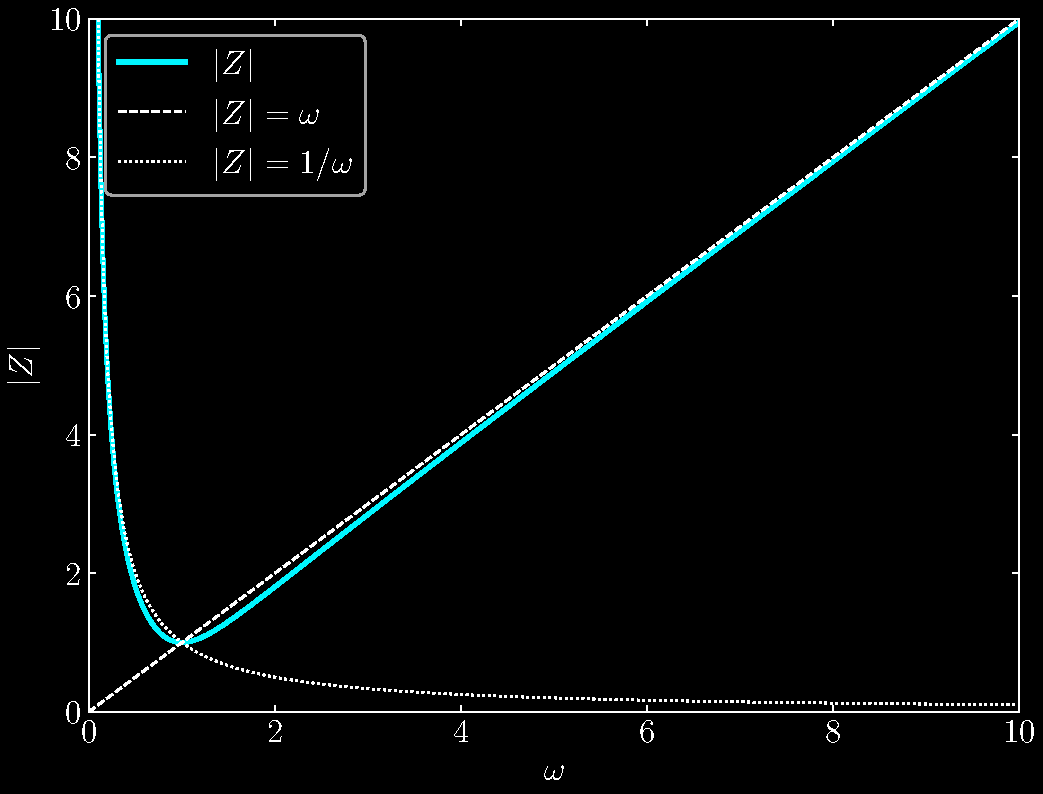
\includegraphics[width=1.0\textwidth]{../chap2/sec2.5/chap2sec2.5ex4.pdf}
\end{center}

\vspace{12pt}

% QUESTION 5
\qs{2.5.5}{Why does an LC loop with no resistor produce a \( 90^{\circ} \) phase shift between current and voltage? Current goes around the loop from a battery of voltage \( V  \) in the loop.}

Conceptually, think of the impedance \( Z \) as the amount by which current is opposed in a circuit. This opposition can come in two forms: resistance or reactance, the real and imaginary components of \( Z \), respectively. Depending on the values of both, the phase difference between current and voltage changes:
\[
	I \!\left( t  \right) = \frac{V }{\abs{Z}} e^{i \!\left( \omega t - \alpha \right)} 
\]
Now, under the premise that \( R \) is zero, we have
\[
	R \rightarrow 0 \quad \implies \quad \tan\!\left(\alpha\right) = \frac{\omega L - 1 / \omega C }{R} \rightarrow \infty 
\]
When \( \tan\!\left(\alpha\right)  \) diverges in this manner, we can conclude that \( \alpha = \pi / 2 \), ascertaining that the phase shift between current and voltage is indeed \( 90^{\circ} \).

\vspace{12pt}

% QUESTION 6
\qs{2.5.6}{The mechanical equivalent of zero resistance is zero damping: \( my'' + ky = \cos\!\left(\omega t \right)  \). Find \( c_{1} \) and \( Y  \) starting from \( y \!\left( 0 \right) = 0 \) and \( y'\!\left( 0 \right) = 0 \) with \( \omega^{2}_{n } = k/m  \).
\[
	y \!\left( t  \right) = c_{1} \cos\!\left(\omega_{n }t \right) + Y \cos\!\left(\omega t \right)  
\]
That answer can be written in two equivalent ways:
\[
	y = Y \!\left( \cos\!\left(\omega t \right) - \cos\!\left( \omega_{n }t \right)  \right) = 2Y \sin\!\left( \frac{\!\left( \omega_{n } - \omega  \right) t }{2} \right) \sin\!\left( \frac{ \!\left( \omega_{n } + \omega \right) t}{2}\right)  
\]}
Substitute \( y_{p } \) into the equation to find
\[
	-m \omega^{2}Y + kY = 1 \quad \implies \boxed{Y = \frac{1}{k - m \omega^{2}}}
\]
From the first initial condition, we deduce
\[
	y \!\left( 0 \right) = c_{1} + Y = 0 \quad \implies \boxed{c_{1} = -Y}
\]
which gives us complete solution
\[
	y \!\left( t  \right) = \frac{\cos\!\left(\omega_{n }t \right) - \cos\!\left(\omega t \right) }{k - m \omega^{2}} 
\]

% QUESTION 7
\qs{2.5.7}{Suppose the driving frequency \( \omega  \) is close to \( \omega_{n } \) in Problem 6. A fast oscillation \( \sin \!\left[ \!\left( \omega_{n } + \omega  \right) t/2 \right] \) is multiplying a very slow oscillation \( 2Y \sin \!\left[ \!\left( \omega_{n } - \omega  \right)t/2 \right] \). By hand or by computer, draw the graph of \( y = \sin\!\left(t \right) \sin\!\left(9t \right)  \) from \( 0 \) to \( 2 \pi  \).

You should see a fast sine curve inside a slow sine curve. This is a \textbf{beat}.}

Suppose that \( \omega \rightarrow \omega_{n } \). Then we can write for the fast oscillation
\[
	\sin \!\left[ \frac{\!\left( \omega_{n } + \omega \right)t }{2} \right] \approx \sin\!\left(\omega_{n }t\right) 
\]
For the slow oscillation, the argument to the sinusoid becomes very small. We can then write the following approximation
\[
	2Y \sin \!\left[ \frac{\!\left( \omega_{n } - \omega \right)t }{2} \right] \approx Y \!\left( \omega_{n } - \omega \right)t 
\]
Taking the product of the approximations, we get
\[
	y \approx Y \!\left( \omega_{n } - \omega \right) t \sin\!\left(\omega_{n } t \right) 
\]
In the numerical example, by inspection we can see that \( \omega_{n } = 10 \) and \( \omega = 8 \), which generates the following graph of the product of oscillations:

\begin{center}
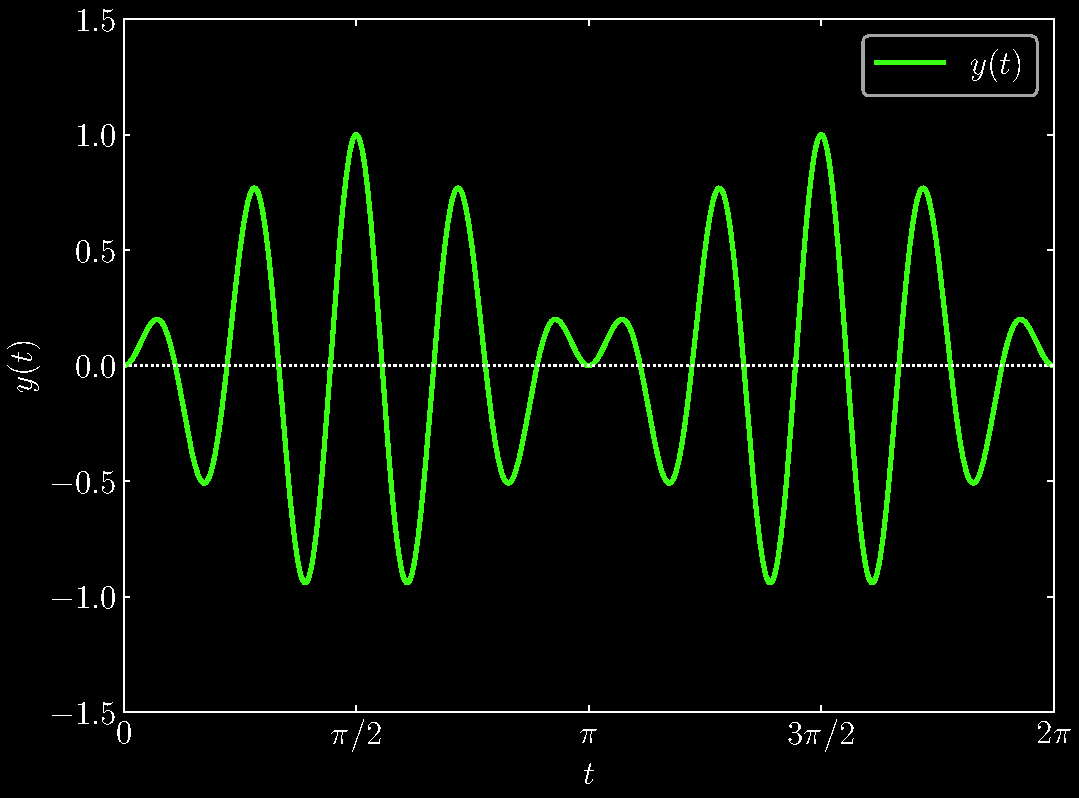
\includegraphics[width=1.0\textwidth]{../chap2/sec2.5/chap2sec2.5ex7.pdf}
\end{center}

But to see the resonance effects as \( \omega \rightarrow \omega_{n } \), consider \( \omega_{n } = 10 \) and \( \omega = 9.9 \). As the delta between them diminishes, the convergence to the resonance solution (\( y_{\text{approx}} \)) becomes apparent:

\begin{center}
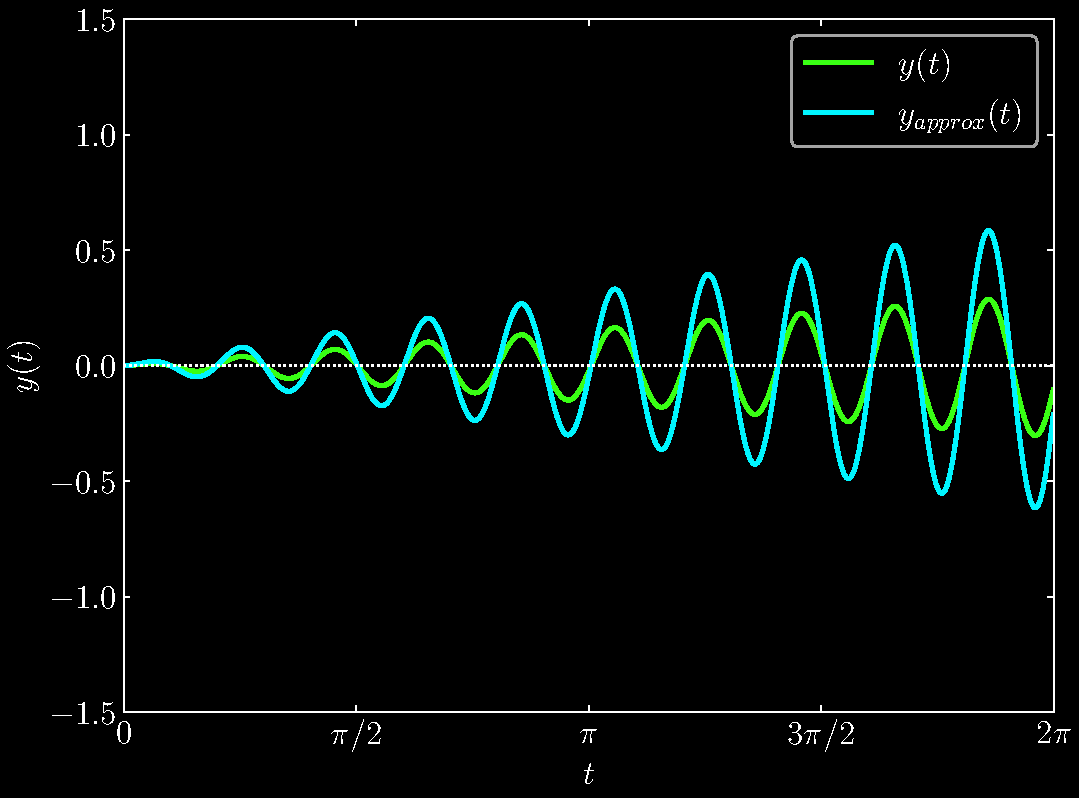
\includegraphics[width=1.0\textwidth]{../chap2/sec2.5/chap2sec2.5ex7a.pdf}
\end{center}

% QUESTION 8
\qs{2.5.8}{What \( m  \), \( b  \), \( k  \), \( F  \) equation for a mass-dashpot-string-force corresponds to Kirchhoff's Voltage Law around a loop? What force balance equation on a mass corresponds to Kirchhoff's Current Law?}

Mass \( m  \) is akin to inductance \( L  \), as both are inertial quantities that resist changes in velocity or electric current, respectively. The damping constant \( b  \) is analogous to circuit resistance \( R  \), as both are measures of the subtractive forces acting on a system's total energy. Lastly, the spring constant \( k  \) serves the function as the reciprocal capacitance \( 1/C  \) -- where \( k  \) quantifies the stiffness of a spring (how hard or easy it is to stretch or compress it), reciprocal capacitance (sometimes called elastance) is a measure of how hard or easy it is to store charge.

In Kirchhoff's Voltage Law, the sum of voltage drops around a closed loop must vanish. It is also the Current Law integrated. The case of the Current Law is perhaps easier to conceptualize: the net sum of current flow at an ode must be zero. In the mechanical analogy, for a multinodal system, every node must have balanced forces.

If we analogize \( y \!\left( t  \right) \) (displacement) to the integral of the current (total distance the charge propagates):
\[
	y \!\left( t  \right) \sim \int I \!\left( t  \right) \, dt
\]
Then the Voltage Law corresponds to the mechanical equation
\[
	my'' + by' + ky = \textbf{applied force} 
\]

% QUESTION 9
\qs{2.5.9}{If you only know the natural frequency \( \omega_{n } \) and the damping coefficient \( b  \) for one mass and one spring, why is that \textit{not enough} to find the damped frequency \( \omega_{d } \)? If you know all of \( m  \), \( b  \), \( k \) what is \( \omega_{d } \)?}

The damped frequency is reliant on the damping ratio \( Z = b / 2 \sqrt{mk} \), namely
\[
	\omega_{d } = \omega_{n } \sqrt{1- Z^{2}} 
\]
Without \( k \), it is impossible to know \( \omega_{d } \).

\vspace{12pt}

% QUESTION 10
\qs{2.5.10}{Varying the number \( a  \) in a first order equation \( y' - ay = 1 \) changes the \textit{speed} of the response. Varying \( B  \) and \( C  \) in a second order equation \( y'' + By' + Cy = 1 \) changes the \textit{form} of the response. Explain the difference.}

The solution to the first order equation is
\[
	y \!\left( t  \right) =\frac{1 - e^{-at }}{a } 
\]
where varying \( a \) alters the rate at which \( y \!\left( t  \right) \) grows while maintaining the specific form of the response. In the case of the second order equation, altering \( B  \) and \( C  \) potentially changes the relationship between \( B^{2} \) and \( 4AC \), which criticaly determines the existence and degree of damping in the equation. Moreover, the natural frequency \( \omega_{n } = \sqrt{C/A } = \sqrt{C } \) is altered.

\vspace{12pt}

% QUESTION 11
\qs{2.5.11}{Find the step response \( r \!\left( t \right) = y_{p } + y_{n } \) for this overdamped system:
\[
	r'' + 2.5r' + r = 1 \text{ with } r \!\left( 0 \right) = 0 \text{ and } r'\!\left( 0 \right) = 0 
\]}

We find \( y_{n } \) and \( y_{p } \) to be
\[
	 r \!\left( t  \right) = 1 + c_{1}e^{-2t } + c_{2}e^{-t/2}
\]
Applying the initial conditions, the coefficients evaluate to
\begin{align*}
	r \!\left( 0 \right) & = 1 + c_{1} + c_{2} = 0 \implies \boxed{c_{1} = -\!\left( 1 + c_{2} \right)} \\
	r'\!\left( 0 \right) & = -2c_{1} - \frac{c_{2}}{2} = 0 \implies \boxed{c_{1} = -\frac{c_{2}}{4}} \\ 
\end{align*}

Leading to \( c_{1} = 1/3 \) and \( c_{2} = -4/3 \), and response
\[
	r \!\left( t  \right) = 1 + \frac{e^{-2t }}{3} - \frac{4e^{-t/2}}{3}
\]

% QUESTION 12
\qs{2.5.12}{Find the step response \( r \!\left( t  \right) = y_{p } + y_{n } \) for this critically damped system. The double root \( s = -1 \) produces what form for the null solution?
\[
	r'' + 2r' + r = 1 \text{ with } r \!\left( 0 \right) = 0 \text{ and } r'\!\left( 0 \right) = 0 
\]}

We have response
\[
	r \!\left( t  \right) = 1 + c_{1}e^{-t } + c_{2} te^{-t } 
\]
which features resonance from the double root. Applying the initial conditions gives us
\begin{align*}
	r \!\left( 0 \right) & = 1 + c_{1} = 0 \implies \boxed{c_{1} = -1} \\
	r'\!\left( 0 \right) & = 1 - c_{1} + c_{2} = 0 \implies \boxed{c_{2} = -2} \\ 
\end{align*}
This gives us final response
\[
	r \!\left( t  \right) = 1 -e^{-t } - 2te^{-t} 
\]

% QUESTION 13
\qs{2.5.13}{Find the step response \( r \!\left( t  \right) \) for this underdamped system using equation (22):
\[
	r'' + r' + r = 1 \text{ with } r \!\left( 0 \right) = 0 \text{ and } r'\!\left( 0 \right) = 0 
\]}

Using equation (22), we first identify \( p  \), \( \omega^{2}_{n } \), and \( \omega_{d } \). Matching the coefficients in the equation, we have
\[
	p = \frac{1}{2}, \quad \omega^{2}_{n } = 1, \quad \omega_{d } = \frac{\sqrt{3}}{2} 
\]
which corresponds to response
\[
	r \!\left( t  \right) = 1 - \frac{2}{\sqrt{3}}e^{-t/2} \sin\!\left( \frac{\sqrt{3}}{2} t + \frac{\pi }{3} \right)  
\]
Note that the phase shift \( \phi = \pi / 3 \) is calculated from \( \phi = \sin^{-1}\!\left( \sqrt{3}/2 \right) = \pi / 3 \).

\vspace{12pt}

% QUESTION 14
\qs{2.5.14}{Find the step response \( r \!\left( t  \right) \) for this undamped system and compare with (22):
\[
	r'' + r = 1 \text{ with } r \!\left( 0 \right) = 0 \text{ and } r'\!\left( 0 \right) = 0 
\]}

Without using equation (22), we identify the null and particular solutions as 
\[
	r \!\left( t  \right) = 1 + c_{1}e^{it } + c_{2}e^{-it } 
\]
Applying the initial conditions gives us
\begin{align*}
	r \!\left( 0 \right) & = 1 + c_{1} + c_{2} \implies \boxed{c_{1} = -\!\left( 1  + c_{2} \right)} \\
	r'\!\left( 0 \right) & = c_{1}i - c_{2}i = 0 \implies \boxed{c_{1} = c_{2}}
\end{align*}
Combined, we have \( c_{1} = c_{2} = -1/2 \), and solution
\[
	r \!\left( t  \right) = 1 - \cos\!\left( t \right)  
\]
Now, using equation (22) gives us parameters \( p = 0 \), \( \omega_{n } = 1 \), \( \omega_{d } = 1 \). From this, we calculate \( \sin\!\left(\phi \right) = 1 \implies \phi = \pi / 2 \), giving us the same solution:
\[
	r \!\left( t  \right) = 1 - \sin\!\left(t + \pi / 2 \right) = 1 - \cos\!\left( t \right) 
\]

% QUESTION 15
\qs{2.5.15}{For \( b^{2} < 4mk \) (underdamping), what parameter decides the speed at which the step response \( r \!\left( t  \right) \) rises to \( r \!\left( \infty \right) = 1 \)? Show that the \textbf{peak time} is \( T = \pi / \omega_{d } \) when \( r \!\left( t  \right) \) reaches its maximum before settling back to \( r = 1 \) at peak time \( r'\!\left( T \right) = 0 \).}

Since we have underdamping (namely, that damping exists), that establishes that \( p \neq 0 \). Then differentiating equation (22) and optimizing the derivative by setting equal to zero, we end up with the following condition:
\[
	\omega_{d } \cos\!\left(\omega_{d } t + \phi \right) = p \sin\!\left(\omega_{d }t + \phi \right)  
\]
Using the fact that \( \omega_{d } / p = \tan\!\left(\phi \right)  \), divide both sides by \( p  \) and the cosine term to derive the clean relation
\[
	\tan\!\left( \phi \right) = \tan\!\left( \omega_{d }t + \phi \right) 
\]
which is true if and only if we have
\[ 
	t = \frac{k \pi }{\omega_{d }} 
\]
For positive integer \( k  \), which presents to us an infinite number of solutions (technically, the oscillation persists forever, even if the amplitude is killed from the exponential decay with time). However, we can only have one solution for the maximum. So let's go with \( k = 1 \), which will be the earliest time as the outer exponential function decays. The peak time, as expected, is derived as 
\[
	T = \frac{\pi }{\omega_{d}} 
\]
The degree to which the response ``stabilizes'' around \( r \!\left( \infty \right) = 1 \) is contingent on \( p  \), which is the decay parameter in \( e^{-pt } \).

\vspace{12pt}

% QUESTION 16
\qs{2.5.16}{If the voltage source \( V \!\left( t  \right) \) in an RLC loop is a unit step function, what resistance \( R  \) will produce an overshoot to \( r_{\text{max}} = 1.2 \) if \( C = 10^{-6} \) Farads and \( L = 1 \) Henry? (Problem 15 found the peak time \( T  \) when \( r \!\left( T  \right) = r_{\text{max}} \)).

Sketch two graphs of \( r \!\left( t  \right) \) for \( p_{1} < p_{2} \). Sketch two graphs as \( \omega_{d } \) increases.}

From the Voltage Law, the differential equation we want to solve is
\[
	y'' + Ry' + 10^{6}y = 1 
\]
and we want \( r_{\text{max}} = 1.2 \). From the previous exercise, we determined that the corresponding time for this maximum response is \( T = \pi / \omega_{d } \). Writing the response in polar form, we have parameters
\[
	p = \frac{R }{2}, \quad \omega^{2}_{n } = 10^{6}, \quad \omega^{2}_{d } = 10^{6} - \frac{R^{2}}{4} \quad \!\left( \frac{1}{\omega^{2}_{d }} = \frac{4}{4 \cdot 10^{6} - R^{2}} \right) 
\]
Now, we substitute \( T  \) in our response function and isolate \( R  \):
\begin{alignat*}{4}
	&& r \!\left( T  \right) && = 1 - \frac{\omega_{n }}{\omega_{d }}e^{-R \pi / 2 \omega_{d }} \sin\!\left( \pi + \phi \right)  & = 1 + \frac{\omega_{n }}{\omega_{d }} e^{-R \pi / 2 \omega_{d }} \frac{\omega_{d }}{\omega_{n }} & \quad \!\left(\text{since } \sin\!\left(\phi \right) = \frac{\omega_{d }}{\omega_{n}} \right)  \\
	&& \implies && r_{\text{max}} = 1.2 & = 1 + e^{-R \pi / 2 \omega_{d}} & \\ 
	&& \implies && \ln\!\left(0.2\right) & = -\frac{R \pi }{2} \!\left( \frac{4}{4 \cdot 10^{6} - R^{2}} \right)^{1/2} & \\
	&& \implies && R^{2} & = \frac{ \ln\!\left(0.2\right)^{2} \cdot 4 \cdot 10^{6}}{\pi^{2} + \ln\!\left(0.2\right)^{2}} & \\
	&& \implies && R & \approx \boxed{912 \ \Omega}
\end{alignat*}

Graphically, \( R_{1} < R_{2} \) implies \( p_{1} < p_{2} \), but \( \omega_{n,1} \) and \( \omega_{n,2} \) are inversely inequal. The lower resistance \( R  \) features higher amplitudes in the oscillation of the response -- less energy is removed from the circuit system than in the case of higher resistance.

\vspace{12pt}

\begin{center}
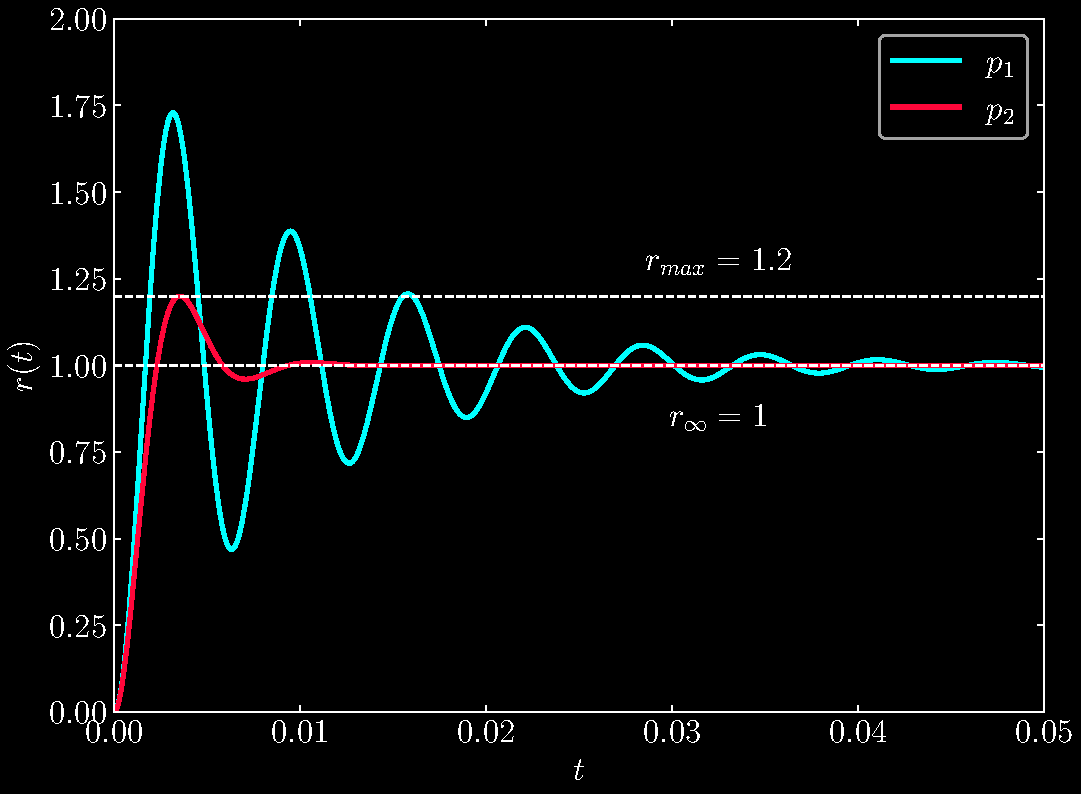
\includegraphics[width=1.0\textwidth]{../chap2/sec2.5/chap2sec2.5ex16.pdf}
\end{center}

\vspace{12pt}

% QUESTION 17
\qs{2.5.17}{What values of \( m  \), \( b  \), \( k  \) will give the step response \( r \!\left( t  \right) = 1 - \sqrt{2}e^{-t } \sin\!\left(t + \frac{\pi }{4}\right) \) ?}

We have
\[
	\frac{\omega_{n }}{\omega_{d }} = \sqrt{2}, \quad p = 1, \quad \omega_{d } = 1 
\]
These relations in turn imply
\[
	\omega^{2}_{n} = \frac{k}{m } = 2, \quad \frac{b }{m } = 2
\]
One choice of parameters that satisfy these relations is \( m = 1 \) and \( b = k = 2 \).

\vspace{12pt}

% QUESTION 18
\qs{2.5.18}{What happens to the \( p - \omega_{d } - \omega_{n } \) right triangle as the damping ratio \( \omega_{n } / p  \) increases to 1 (critical damping)? At that point the damped frequency \( \omega_{d } \) becomes \underline{\qquad}. The step response becomes \( r \!\left( t  \right) = \underline{\qquad} \).}

We have damped frequency \( \omega_{d } = 0 \), which implies that we have repeated roots \( s_{1,2} = p  \) and \( p = \omega_{n } \). Because of resonance, our solution changes to be 
\[
	r \!\left( t  \right) = 1 + c_{1}e^{-pt } + c_{2}te^{-pt } 
\]
Applying the initial conditions \( r \!\left( 0 \right) \) and \( r'\!\left( 0 \right) \) give us coefficients \( c_{1} = -1 \) and \( c_{2} = -p  \). Assembling it all together, our solution is
\[
	r \!\left( t  \right) = 1 - e^{-pt } \!\left( 1 + pt \right) 
\]

% QUESTION 19
\qs{2.5.19}{\textbf{The roots \( \pmb{s_{1}, s_{2} = -p \pm i \omega_{d }} \) are poles of the transfer function \( \pmb{1 / \!\left( As^{2} + Bs + C  \right)} \)}

Show directly that the product of the roots \( s_{1} = -p + i \omega_{d } \) and \( s_{2} = -p - i \omega_{d } \) is \( s_{1}s_{2} = \omega^{2}_{n } \). The sum of the roots is \( -2p \). The quadratic equation with those roots is \( s^{2} + 2ps + \omega^{2}_{n } = 0 \).}

The product is
\[
	s_{1}s_{2} = \!\left( -p + i \omega_{d } \right)\!\left( -p - i \omega_{d } \right) = p^{2} + \omega^{2}_{d} = \omega^{2}_{n}
\]
The imaginary components cancel in the sum, giving us \( s_{1} + s_{2} = -2p \). These relations are Vieta's formulas for a quadratic, where the sum of the roots equals \( -B/A  \) and their product \( C/A  \).

\vspace{12pt}

% QUESTION 20
\qs{2.5.20}{Suppose \( p  \) is increased while \( \omega_{n } \) is held constant. How do the roots \( s_{1} \) and \( s_{2} \) move?}

The imaginary component \( \omega_{d } \) decreases in magnitude, meaning that the roots move along the circle of radius \( \omega_{n } \) on the complex plane towards the negative real axis at \(-p \rightarrow -\omega_{n } \).

\vspace{12pt}

% QUESTION 21
\qs{2.5.21}{Suppose the mass \( m  \) is increased while the coefficients \( b  \) and \( k \) are unchanged. What happens to the roots \( s_{1} \) and \( s_{2} \)?}

All else equal, increasing the mass \( m  \) means that the roots move inward onto a complex circle of smaller radius, approaching zero in the limit. Since the roots are expressed as 
\[
	s = -\frac{b }{2m} \pm \frac{\sqrt{b^{2} - 4mk}}{2m}
\]
We can see that increasing \( m  \) will eventually force the second term to be imaginary, even as the real and imaginary components in magnitude diminish. Importantly, \( \omega^{2}_{n} = k/m \) 

Intuitively, we imagine a heavy mass-dashpot-spring system. The natural frequency \( \omega_{n } \) will drastically decrease, indicating the increasingly slow oscillation of the mass. Since the damping coefficient is unchanged, the damping per unit mass is increasingly washed out with a heavier mass, indicating a proportionally lower amount of energy loss given an input forcing.

\vspace{12pt}

\newpage
% QUESTION 22
\qs{2.5.22}{\textbf{Ramp response} How could you find \( y \!\left( t  \right) \) when \( F = t  \) is a ramp function?

\[
	y'' + 2py' + \omega^{2}_{n }y = \omega^{2}_{n }t \text{ starting from } y \!\left( 0 \right) = 0 \text{ and } y'\!\left( 0 \right) = 0 
\]
A particular solution (straight line) is \( y_{p } =  \) \underline{\qquad}. The null solution still has the form \( y_{n} =  \) \underline{\qquad}. Find the coefficients \( c_{1} \) and \( c_{2} \) in the null solution from the two conditions at \( t = 0 \).

This ramp response \( y \!\left( t \right) \) can also be seen as the integral of \underline{\qquad}.}

The particular solution is \( y_{p } = t - 2p / \omega^{2}_{n} \). The null solution has form \( y_{n } = c_{1}e^{s_{1}t } + c_{2}e^{s_{2}t } \), where the roots are
\[
	s_{1,2} = -p \pm \sqrt{p^{2} - \omega^{2}_{n }} = -p \pm i \omega_{d} 
\]
This gives us complete solution
\[
	y \!\left( t  \right) = c_{1}e^{s_{1}t } + c_{2}e^{s_{2}t } + t - \frac{2p}{\omega^{2}_{n}}
\]
To find the coefficients, apply the initial conditions and derive
\begin{align*}
	y \!\left( 0 \right) & = c_{1} + c_{2} - \frac{2p}{\omega^{2}_{n}} = 0 \implies \boxed{c_{1} = \frac{2p}{\omega^{2}_{n}} - c_{2}} \\[12pt]
	y'\!\left( 0 \right) & = c_{1}s_{1} + c_{2}s_{2} + 1 = 0 \implies \boxed{c_{2} = \frac{1 + \frac{2p}{\omega^{2}_{n}}s_{1}}{s_{1} - s_{2}}}
\end{align*}
which then implies
\[
	\boxed{c_{1} = \frac{1 + \frac{2p}{\omega^{2}_{n}}s_{2}}{s_{2} - s_{1}} }
\]
The ramp response (slanted line) is the integral of the step response (horizontal line). 

\newpage
\subsection{\textsf{2.6 - Solutions to Second Order Equations}}

\textbf{Find a particular solution by inspection} (or the method of undetermined coefficients)

\vspace{12pt}

% QUESTION 1
\qs{2.6.1}{
\begin{enumerate}[label=(\alph*)]
	\item \( y'' + y = 4 \)
	\item \( y'' + y' = 4 \)
	\item \( y'' = 4 \)
\end{enumerate}}

\begin{enumerate}[label=(\alph*)]
	\item \( y_{p } = 4 \)
	\item \( y_{p } = 4t \)
	\item \( y_{p } = 2t^{2} \)
\end{enumerate}

% QUESTION 2
\qs{2.6.2}{
\begin{enumerate}[label=(\alph*)]
	\item \( y'' + y' + y = e^{t } \)
	\item \( y'' + y' + y = e^{ct } \)
\end{enumerate}}

\begin{enumerate}[label=(\alph*)]
	\item \( y_{p } = \frac{1}{3}e^{t } \)
	\item Substitute \( y_{p } = Ye^{ct } \) to find
	\[
	      c^{2}Y + cY + Y = 1 \implies Y = \frac{1}{c^{2} + c + 1}
	\]
\end{enumerate}

% QUESTION 3
\qs{2.6.3}{
\begin{enumerate}[label=(\alph*)]
	\item \( y'' - y  =\cos\!\left(t \right)  \)
	\item \( y'' + y = \cos\!\left(2t \right)  \)
	\item \( y'' + y = t + e^{t } \)
\end{enumerate}}

\begin{enumerate}[label=(\alph*)]
	\item Substitute \( y_{p } = Y\cos\!\left(t \right)  \) to find
	\[
		 -2Y \cos\!\left(t \right) = \cos\!\left(t \right) \implies Y = -\frac{1}{2}
	\]
	\item Substitute \( y_{p } = Y \cos\!\left(2t\right)  \) to find
	\[
		-3Y \cos\!\left(2t\right)  = \cos\!\left(2t\right) \implies Y = -\frac{1}{3}
	\]
	\item \( y_{p } = t + \frac{1}{2}e^{t} \)
\end{enumerate}

% QUESTION 4
\qs{2.6.4}{For these \( f \!\left( t  \right) \), predict the form of \( y \!\left( t  \right) \) with undetermined coefficients:
\begin{enumerate}[label=(\alph*)]
	\item \( f \!\left( t  \right) = t^{3} \)
	\item \( f \!\left( t  \right) = \cos\!\left(2t\right)  \)
	\item \( f \!\left( t  \right) = t \cos\!\left(t \right)  \)
\end{enumerate}}

\begin{enumerate}[label=(\alph*)]
	\item \( y_{p } \!\left( t  \right) = at^{3} + bt^{2} + ct + d  \)
	\item \( y_{p } \!\left( t  \right) = a \cos\!\left(2t\right) + b \sin\!\left(2t\right)  \)
	\item \( y_{p } \!\left( t  \right) = \!\left( at + b  \right) \cos\!\left(t \right) + \!\left( ct + d  \right) \sin\!\left(t \right) \)
\end{enumerate}

% QUESTION 5
\qs{2.6.5}{Predict the form for \( y \!\left( t  \right) \) when the right hand side is
\begin{enumerate}[label=(\alph*)]
	\item \( f \!\left( t  \right) = e^{ct } \)
	\item \( f \!\left( t  \right) = te^{ct } \)
	\item \( f \!\left( t  \right) = e^{t }\cos\!\left(t \right) \)
\end{enumerate}}

\begin{enumerate}[label=(\alph*)]
	\item \( y_{p } \!\left( t  \right) = Ye^{ct } \)
	\item \( y_{p } \!\left( t  \right) = \!\left( at + b  \right)e^{ct } \)
	\item \( y_{p } \!\left( t  \right) = e^{t } \!\left( a \cos\!\left(t \right) + b \sin\!\left(t \right)  \right) \)
\end{enumerate}

% QUESTION 6
\qs{2.6.6}{For \( f \!\left( t  \right) = e^{ct } \) when is the prediction for \( y \!\left( t  \right) \) different from \( Ye^{ct } \)?}

If \( e^{ct } \) is one of the null solutions, we must have a \( Yte^{ct } \) term to account for the resonance.

\vspace{12pt}

\textbf{Use the method of undetermined coefficients to find a solution \( \pmb{y_{p } \!\left( t  \right)} \).}

\vspace{12pt}

% QUESTION 7
\qs{2.6.7}{
\begin{enumerate}[label=(\alph*)]
	\item \( y'' + 9y = e^{2t} \)
	\item \( y'' + 9y = te^{2t} \)
\end{enumerate}}

\begin{enumerate}[label=(\alph*)]
	\item Let \( y_{p } \!\left( t  \right) = Ye^{2t} \). Then
	\[
		4Ye^{2t} + 9Ye^{2t} = e^{2t} \implies Y = \frac{1}{13} \implies y_{p } \!\left( t  \right) = \frac{e^{2t}}{13}
	\]
	\item Let \( y_{p } \!\left( t  \right) = \!\left( at + b  \right)e^{2t} \). Then 
	\begin{align*}
		y_{p }' \!\left( t  \right) & = ae^{2t} + 2 \!\left( at + b  \right)e^{2t} \\
					    & = \!\left( 2at + a + 2b \right)e^{2t} \\ 
		y_{p }''\!\left( t  \right) & = 2ae^{2t} + 2 \!\left( 2at + a + 2b \right)e^{2t} \\
					    & = \!\left( 4at + 4a + 4b \right)e^{2t}
	\end{align*}
	Substituting into the equation, we derive
	\[
		\!\left( 4at + 4a + 4b \right)e^{2t} + 9 \!\left( at + b  \right)e^{2t} = \!\left( 13at  + 4a + 13b \right)e^{2t} = te^{2t}
	\]
	Here, we can deduce that \( a = \displaystyle{\frac{1}{13}} \) and \( b = \displaystyle{-\frac{4}{13}\frac{1}{13}} \). Our particular solution is
	\[
		y_{p } \!\left( t  \right) = \frac{1}{13}\!\left( t - \frac{4}{13} \right)e^{2t} 
	\]
\end{enumerate}

% QUESTION 8
\qs{2.6.8}{
\begin{enumerate}[label=(\alph*)]
	\item \( y'' + y' = t + 1 \)
	\item \( y'' + y' = t^{2} + 1 \)
\end{enumerate}}

\begin{enumerate}[label=(\alph*)]
	\item Observe that the roots of the characteristic polynomial are \( s = 0, -1 \). Then one of the null solutions is simply a constant, so that cannot be present in our particular solution. Let \( y_{p } \!\left( t  \right) = at^{2} + bt \) (no constant term). Then
		\begin{align*}
			y'\!\left( t  \right) & = 2at + b  \\
			y''\!\left( t  \right) & = 2a
		\end{align*}
	Substituting, we get
	\[
		2at + \!\left( 2a + b  \right) = t + 1 
	\]
	Where we can conclude \( a = 1/2 \) and \( b = 0 \), and
	\[
		y_{p } \!\left( t  \right) = \frac{1}{2}t^{2} 
	\]
	\item The equation is the same but the forcing changes, so we have ansatz \( y_{p } \!\left( t  \right) = at^{3} + bt^{2} + ct  \) (again, no constant term). Then
		\begin{align*}
			y'\!\left( t  \right) & = 3at^{2} + 2bt + c  \\[12pt]
			y''\!\left( t  \right) & = 6at + 2b
		\end{align*}
	We substitute to get
	\[
		3at^{2} + \!\left( 6a + 2b \right)t + 2b + c = t^{2} + 1 
	\]
	Concluding that \( a = 1/3 \), \( b = -1 \), and \( c = 2 \). This corresponds to particular solution
	\[
		y_{p }\!\left( t  \right) = \frac{1}{3}t^{3} - t^{2} + 2t 
	\]
\end{enumerate}

% QUESTION 9
\qs{2.6.9}{
\begin{enumerate}[label=(\alph*)]
	\item \( y'' + 3y = \cos\!\left(t \right)  \)
	\item \( y'' + 3y = t \cos\!\left(t \right)  \)
\end{enumerate}}

\begin{enumerate}[label=(\alph*)]
	\item Let \( y_{p } \!\left( t  \right) = a \cos\!\left(t \right) + b \sin\!\left(t \right)  \). Substituting gives us
	\[
		2a \cos\!\left(t \right) + 2b \sin\!\left(t \right) = \cos\!\left(t \right)  
	\]
	From which we can deduce \( a = 1/2 \) and \( b = 0 \), yielding solution
	\[
		y_{p } \!\left( t  \right) = \frac{1}{2}\cos\!\left(t \right)  
	\]
	\item Let \( y_{p } \!\left( t  \right) = \!\left( at + b  \right)\cos\!\left(t \right) + \!\left( ct + d  \right) \sin\!\left(t \right)   \). Then
	\begin{align*}
		y'_{p} \!\left( t  \right) & = a \cos\!\left(t \right) - \!\left( at + b  \right) \sin\!\left(t \right) +c \sin\!\left(t \right) + \!\left( ct + d  \right) \cos\!\left(t \right) \\
					   & = \!\left( ct + a + d  \right) \cos\!\left(t \right) + \!\left( -at - b + c  \right) \sin\!\left(t \right) \\
		y''_{p } \!\left( t  \right) & = c \cos\!\left(t \right) - \!\left( ct + a + d  \right) \sin\!\left(t \right) - a \sin\!\left(t \right) + \!\left( -at - b + c  \right) \cos\!\left(t \right) \\
					     & = \!\left( -at - b + 2c \right) \cos\!\left(t \right) - \!\left( ct + 2a + d \right) \sin\!\left(t \right) 
	\end{align*}
	Substituting gives us
	\[
		 \!\left( 2at + 2b + 2c \right) \cos\!\left(t \right) + \!\left( 2ct - 2a + 2d \right) \sin\!\left(t \right) = t \cos\!\left(t \right) 
	\]
	We must have \( a = d - 1/2 \) and \( b = c = 0 \), which corresponds to particular solution
	\[
		y_{p } \!\left( t  \right) = \frac{1}{2}t \cos\!\left(t \right) + \frac{1}{2} \sin\!\left(t \right)  
	\]
\end{enumerate}

% QUESTION 10
\qs{2.6.10}{
\begin{enumerate}[label=(\alph*)]
	\item \( y'' + y' + y = t^{2} \)
	\item \( y'' + y' + y = t^{3} \)
\end{enumerate}}

\begin{enumerate}[label=(\alph*)]
	\item Let \( y_{p } \!\left( t  \right) = at^{2} + bt + c  \). Then \( y_{p}'\!\left( t \right) = 2at + b  \) and \( y_{p }''\!\left( t  \right) = 2a \). Substituting yields
	\[
		at^{2} + \!\left( 2a + b  \right)t + 2a + b + c = t^{2} 
	\]
	where we can deduce that \( a = 1 \), \( b = -2 \), and \( c = 0 \), and solution
	\[
		y_{p } \!\left( t  \right) = t^{2} - 2t
	\]
	\item Let \( y_{p } \!\left( t  \right) = at^{3} + bt^{2} + ct + d  \). Then \( y_{p }'\!\left( t  \right) = 3at^{2} + 2bt + c  \) and \( y_{p }''\!\left( t  \right) = 6at + 2b \). Substituting yields
	\[
		 at^{3} + \!\left( 3a + b  \right)t^{2} + \!\left( 6a + 2b + c  \right)t + 2b + c + d = t^{3}
	\]
	which gives us coefficients \( a = 1 \), \( b = -3 \), \( c = 0 \), and \( d = 6 \). We have particular solution
	\[
		y_{p } \!\left( t  \right) = t^{3} - 3t^{2} + 6 
	\]
\end{enumerate}

% QUESTION 11
\qs{2.6.11}{
\begin{enumerate}[label=(\alph*)]
	\item \( y'' + y' + y = \cos\!\left(t \right)  \)
	\item \( y'' + y' + y = t \sin\!\left(t \right)  \)
\end{enumerate}}

\begin{enumerate}[label=(\alph*)]
	\item Let \( y_{p } \!\left( t  \right) = a \cos\!\left(t \right) + b \sin\!\left(t \right)  \). Then \( y_{p }'\!\left( t  \right) = -a \sin\!\left(t \right) + b \cos\!\left(t \right)  \) and \( y_{p }''\!\left( t  \right) = -a \cos\!\left(t \right) - b \sin\!\left(t \right)  \). Substituting gives us
	\[
		-a \sin\!\left(t \right) + b \cos\!\left(t \right) = \cos\!\left(t \right)  
	\]
	which has \( a = 0 \) and \( b = 1 \), with solution \( y_{p } \!\left( t  \right) = \sin\!\left(t \right)  \).
	\item Let \( y_{p } \!\left( t  \right) = \!\left( at + b  \right)\cos\!\left(t \right) + \!\left( ct + d  \right)\sin\!\left(t \right)  \). Then
	\begin{align*}
		y_{p }'\!\left( t  \right) & = a \cos\!\left(t \right) - \!\left( at + b  \right)\sin\!\left(t \right) + c \sin\!\left(t \right) + \!\left( ct + d  \right)\cos\!\left(t \right)  \\
					   & = \!\left( ct + a + d  \right)\cos\!\left(t \right) + \!\left( -at - b + c  \right)\sin\!\left(t \right) \\
		y_{p }''\!\left( t  \right) & = c \cos\!\left(t \right) - \!\left( ct + a + d  \right) \sin\!\left(t \right) - a \sin\!\left(t \right) + \!\left( -at - b + c  \right) \cos\!\left(t \right)  \\ 
					    & = \!\left( -at - b + 2c \right) \cos\!\left(t \right) + \!\left( -ct - 2a - d  \right) \sin\!\left(t \right) 
	\end{align*}
	Substituting gives us
	\[
		\!\left( ct + a + 2c + d  \right) \cos\!\left(t \right) + \!\left( -at - b - 2a + c  \right) \sin\!\left(t \right) = t \sin\!\left(t \right)  
	\]
	This forces \( c = 0 \), \( a = -1 \), \( d = 1 \), and \( b = 2 \), which corresponds to solution
	\[
		y_{p } \!\left( t  \right) = \!\left( -t + 2 \right)\cos\!\left(t \right) + \sin\!\left(t \right)  
	\]
\end{enumerate}

\textbf{Problems 12-14 involve resonance. Multiply the usual form of \( \pmb{y_{p}} \) by \( \pmb{t} \).}

\vspace{12pt}

% QUESTION 12
\qs{2.6.12}{
\begin{enumerate}[label=(\alph*)]
	\item \( y'' + y = e^{it } \)
	\item \( y'' + y = \cos\!\left(t \right)  \)
\end{enumerate}}

\begin{enumerate}[label=(\alph*)]
	\item Let \( y_{p } \!\left( t  \right) = Yte^{it } \). Then \( y_{p }'\!\left( t  \right) = Y \!\left( e^{it } + ite^{it } \right) = Y \!\left( 1 + it  \right)e^{it } \) and \( y_{p }''\!\left( t  \right) = Y \!\left( ie^{it } + \!\left( i - t  \right)e^{it } \right) = Y \!\left( 2i - t  \right)e^{it} \). Substituting gives us
	\[
		2iYe^{it } = e^{it } \implies Y = -\frac{i }{2} 
	\]
	which corresponds to solution
	\[
		y_{p } \!\left( t  \right) = -\frac{i }{2}te^{it } 
	\]
	\item Let \( y_{p } \!\left( t  \right) = t \!\left( a \cos\!\left(t \right) + b \sin\!\left(t \right)  \right) \). Then
	\begin{align*}
		y_{p }'\!\left( t  \right) & = a \cos\!\left(t \right) + b \sin\!\left(t \right) + t \!\left( -a \sin\!\left(t \right) + b \cos\!\left( t \right)  \right) \\
					   & = \!\left( bt + a  \right)\cos\!\left(t \right) + \!\left( -at + b  \right)\sin\!\left(t \right) \\
		y_{p }''\!\left( t  \right) & = b \cos\!\left(t \right) - \!\left( bt + a  \right) \sin\!\left(t \right) - a \sin\!\left(t \right) + \!\left( -at + b  \right) \cos\!\left(t \right) \\ 
					    & = \!\left( -at + 2b \right) \cos\!\left(t \right) - \!\left( bt + 2a \right) \sin\!\left( t \right)
	\end{align*}
	Substituting gives us
	\[
		2b \cos\!\left(t \right) - 2a \sin\!\left(t \right) = \cos\!\left(t \right)  
	\]
	Forcing \( a = 0 \) and \( b = 1/2 \), and solution
	\[
		y_{p } \!\left( t  \right) = \frac{1}{2}t \sin\!\left(t\right) 
	\]
\end{enumerate}

% QUESTION 13
\qs{2.6.13}{
\begin{enumerate}[label=(\alph*)]
	\item \( y'' - 4y' + 3y = e^{t } \)
	\item \( y'' - 4y' + 3y = e^{3t} \)
\end{enumerate}}

\begin{enumerate}[label=(\alph*)]
	\item Let \( y_{p } \!\left( t  \right) = Yte^{t } \). Then \( y_{p }'\!\left( t  \right) = Y \!\left( e^{t } + te^{t } \right) \) and \( y_{p }''\!\left( t  \right) = Y \!\left( 2e^{t } + te^{t} \right) \). Substituting gives us
	\[
		-2Ye^{t } = e^{t } \implies Y = -\frac{1}{2}
	\]
	which corresponds to solution
	\[
		y_{p } \!\left( t  \right) = -\frac{1}{2}te^{t} 
	\]
	\item Let \( y_{p } \!\left( t  \right) = Yte^{3t} \). Then \( y_{p }'\!\left( t  \right) = Y \!\left( e^{3t} + 3te^{3t} \right) \) and \( y_{p }''\!\left( t  \right) = Y \!\left( 6e^{3t} + 9te^{3t} \right) \). Substituting gives us
	\[
		2Ye^{3t} = e^{3t} \implies Y = \frac{1}{2}
	\]
	which corresponds to solution
	\[
		y_{p } \!\left( t  \right) = \frac{1}{2}te^{3t} 
	\]
\end{enumerate}

% QUESTION 14
\qs{2.6.14}{
\begin{enumerate}[label=(\alph*)]
	\item \( y' - y = e^{t } \)
	\item \( y' - y = te^{t } \)
	\item \( y' - y = e^{t } \cos\!\left(t\right)  \)
\end{enumerate}}

\begin{enumerate}[label=(\alph*)]
	\item Let \( y_{p } \!\left( t  \right) = Yte^{t } \). Then \( y_{p }'\!\left( t  \right) = Y \!\left( e^{t } + te^{t } \right) \). Then we substitute to derive
	\[
		Ye^{t } = e^{t } \implies Y = 1 
	\]
	Then we have \( y_{p } \!\left( t  \right) = te^{t } \).
	\item Let \( y_{p } \!\left( t  \right) = Yt^{2}e^{t } \). Then \( y_{p }'\!\left( t  \right) = Y \!\left( t^{2}e^{t } + 2te^{t } \right) \). We substitute to get
	\[
		2Yte^{t } = te^{t } \implies Y = \frac{1}{2} 
	\]
	Our solution is
	\[
		y_{p } \!\left( t  \right) = \frac{1}{2}t^{2}e^{t }
	\]
	\item Let \( y_{p }\!\left( t  \right) = e^{t } \!\left( a \cos\!\left(t \right) + b \sin\!\left(t \right)  \right) \). Then 
	\begin{align*}
		y_{p}'\!\left( t \right) & = e^{t}\!\left[ \!\left( a \cos\!\left(t \right) + b \sin\!\left(t \right)  \right) + \!\left( -a \sin\!\left(t \right) + b \cos\!\left(t \right)  \right) \right] \\
					 & = e^{t } \!\left[ \!\left( a + b  \right)\cos\!\left(t \right) + \!\left( b - a  \right) \sin\!\left(t \right)  \right]
	\end{align*}
	We substitute to get
	\[
		e^{t } \!\left( b \cos\!\left(t \right) - a \sin\!\left(t \right)  \right) = e^{t } \cos\!\left(t \right)  \implies a = 0, b = 1
	\]
	Therefore our solution is
	\[
		y_{p }\!\left( t  \right) = e^{t }\sin\!\left(t\right)  
	\]
\end{enumerate}

% QUESTION 15
\qs{2.6.15}{For \( y'' - 4y = e^{t }\sin\!\left(t \right)  \) (exponential times sinusoidal) we have two choices:
\begin{alignat*}{2}
	\textbf{1} \quad & \text{(Real)} && \quad \text{Substitute } y_{p } = Me^{t } \cos\!\left(t \right) + Ne^{t }\sin\!\left(t \right): \\
		   & 		   && \quad \text{determine } M \text{ and } N \\
	\textbf{2} \quad & \text{(Complex)} && \quad \text{Solve } z'' + 4z = e^{\!\left( 1 + i  \right)t }. \\
		   &                  && \quad \text{Then } y \text{ is the imaginary part of } z. 
\end{alignat*}
Use both methods to find the same \( y \!\left( t  \right) \) -- which do you prefer?}

\begin{enumerate}[label=\arabic*.]
	\item Let \( y_{p } \) be as given. Then
	\begin{align*}
		y'_{p } & = Me^{t} \!\left( \cos\!\left(t \right) - \sin\!\left(t \right)  \right) + Ne^{t} \!\left( \sin\!\left(t \right) + \cos\!\left(t\right)  \right)  \\
		y''_{p} & = -2Me^{t} \sin\!\left(t \right) + 2Ne^{t} \cos\!\left(t\right) 
	\end{align*}
	Substituting gives us
	\[
		e^{t } \!\left[ \!\left( 2N - 4M \right)e^{t }\cos\!\left(t \right) - \!\left( 2M + 4N \right)\sin\!\left(t\right) \right] = e^{t }\sin\!\left(t\right) 
	\]
	We must have \( -4M + 2N = 0 \) and \( -\!\left( 2M + 4N \right) = 1 \). Solve the matrix equation:
	\[
		\begin{bmatrix}
			-4 & 2\\
			-2 & -4\\
		\end{bmatrix}
		\begin{bmatrix}
			M \\
			N \\
		\end{bmatrix} = 
		\begin{bmatrix}
			1 \\
			0 \\
		\end{bmatrix}
	\]
	Which gives us \( M = -1/5 \) and \( N = 1/10 \).
	\item In the complex case, let \( y_{p } = Ye^{\!\left( 1 + i  \right)t} \). Then \( y'_{p } = Y \!\left( 1 + i  \right)e^{\!\left( 1 + i  \right)t } \) and \( y''_{p } = Y \!\left( 1 + i  \right)^{2}e^{\!\left( 1 + i  \right)t } \), and our task reduces to isolating \( Y  \) in the equation
	\[
		Y \!\left( 1 + i  \right)^{2} - 4Y \!\left( 1 + i  \right) = 1 
	\]
	Doing so yields
	\[
		Y = -\frac{1}{4 + 2i} = \frac{-4 + 2i}{20} = \frac{-2 + i }{10}
	\]
	Our particular solution is
	\begin{align*}
		y_{p } & = \!\left( \frac{-2 + i}{10} \right) e^{t} \!\left( \cos\!\left(t \right) + i \sin\!\left(t\right)  \right) \\
		       & = -\frac{1}{5} e^{t }\cos\!\left(t \right) + \frac{1}{10}e^{t }\sin\!\left(t \right) + i \!\left[ \frac{1}{10}e^{t }\cos\!\left(t \right) - \frac{1}{5}e^{t }\sin\!\left(t\right)  \right]
	\end{align*}
	Taking the real component, we see that it matches with what we had in part 1.
\end{enumerate}

% QUESTION 16
\qs{2.6.16}{
\begin{enumerate}[label=(\alph*)]
	\item Which values of \( c  \) give resonance for \( y'' + 3y' - 4y = te^{ct } \)?
	\item What form would you substitute for \( y \!\left( t  \right) \) if there is no resonance?
	\item What form would you use when \( c  \) produces resonance?
\end{enumerate}}

\begin{enumerate}[label=(\alph*)]
	\item The characteristic polynomial is \( s^{2} + 3s - 4 \) which has roots \( s_{1} = -4 \) and \( s_{2} = 1 \), so those values of \( c  \) will give resonance. This is because our ansatz, when of the form \( y_{p } = \!\left( at + b  \right)e^{ct } \), includes the form of the null solutions.
	\item If no resonance, then we can safely put forth our ansatz with the form \( y_{p }= \!\left( at + b  \right)e^{ct } \).
	\item Otherwise, use form \( y_{p } = \!\left( at^{2} + bt  \right)e^{ct } \).
\end{enumerate}

% QUESTION 17
\qs{2.6.17}{This is the rule for equations \( P \!\left( D  \right)y = e^{ct } \) with resonance \( P \!\left( c  \right) = 0 \):

If \( P \!\left( c  \right) = 0 \) and \( P'\!\left( c  \right) \neq 0 \), look for a solution \( y_{p } = Cte^{ct } \) (\( m = 1 \))

If \( c  \) is a root of multiplicity \( m  \), then \( y_{p } \) has the form \underline{\qquad}.}

Then \( y_{p } \) has form \( Ct^{m }e^{ct } \).

\vspace{12pt}

\newpage
% QUESTION 18
\qs{2.6.18}{
\begin{enumerate}[label=(\alph*)]
	\item To solve \( d^{4}y / dt^{4} - y = t^{3}e^{5t} \), what form do you expect for \( y \!\left( t  \right) \)?
	\item If the right side becomes \( t^{3}\cos\!\left(5t\right)  \), which 8 coefficients are to be determined?
\end{enumerate}}

\begin{enumerate}[label=(\alph*)]
	\item The characteristic polynomial is \( s^{4} - 1 \), which gives us roots \( s = \pm 1, \pm i  \). Since \( c = 5 \), we need not concern ourselves with resonance, and we guess \( y_{p } = \!\left( at^{3} + bt^{2} + ct + d  \right)e^{5t} \).
	\item In this case, we then determine the number of combinations between sine and cosine and the four terms of a third-degree polynomial:
	\begin{alignat*}{3}
		t^{3}\cos\!\left(5t \right) & \quad t^{2}\cos\!\left(5t \right) & \quad t\cos\!\left(5t \right) & \quad \cos\!\left(5t \right)  \\
		t^{3}\sin\!\left(5t \right) & \quad t^{2}\sin\!\left(5t \right) & \quad t \sin\!\left(5t \right) & \quad \sin\!\left(5t \right)  \\ 
	\end{alignat*}
\end{enumerate}

% QUESTION 19
\qs{2.6.19}{For \( y' - ay = f \!\left( t  \right) \), the method of undetermined coefficients is looking for all \( f \!\left( t  \right) \) so that the usual formula \( y_{p } = e^{at } \int e^{-as } f \!\left( s  \right) \, ds  \) is easy to integrate. Find these integrals for the ``nice functions'' \( f = e^{ct } \), \( f = e^{i \omega t } \), and \( f = t  \):
\[
	\int e^{-as }e^{cs}  \, ds \qquad \int e^{-as } e^{i \omega s } \, ds \qquad \int e^{-as }s \, ds
\]}

\begin{enumerate}[label=(\alph*)]
	\item 
	\[
		\int e^{-as }e^{cs } \, ds = \int e^{\!\left( -a + c  \right)s } \, ds = \frac{e^{\!\left( -a + c  \right)s }}{-a + c } + C
	\]
	\item 
	\[
		\int e^{-as }e^{i \omega s } \, ds = \int e^{\!\left( -a + i \omega  \right)s } \, ds = \frac{e^{\!\left( -a + i \omega  \right)s }}{-a + i \omega } + C
	\]
	\item 
	Resort to integration by parts. Let \( u = s  \) and \( dv = e^{-as } ds  \). Then \( du = ds  \) and \( v = -e^{-as } / a \).
	\[
		\int e^{-as }s \, ds = -\frac{e^{-as }s }{a } + \frac{1}{a } \int e^{-as } \, ds = -e^{-as } \!\left( \frac{s }{a } + \frac{1}{a^{2}} \right)
	\]
\end{enumerate}

\vspace{12pt}

\newpage
\textbf{Problems 20-27 develop the method of variation of parameters.}

\vspace{12pt}

% QUESTION 20
\qs{2.16.20}{Find two solutions \( y_{1} \), \( y_{2} \) to \( y'' + 3y' + 2y = 0 \). Use those in formula (13) to solve
\begin{enumerate}[label=(\alph*)]
	\item \( y'' + 3y' + 2y = e^{t } \)
	\item \( y'' + 3y' + 2y = e^{-t } \)
\end{enumerate}}

\begin{enumerate}[label=(\alph*)]
	\item The roots to the characteristic polynomial are \( s_{1,2} = -2, -1 \). Then we have null solutions \( y_{1} = e^{-2t} \) and \( y_{2} = e^{-t } \), and correspondingly \( y'_{1} = -2e^{-2t} \) and \( y'_{2} = -e^{-t } \). The Wronskian is calculated as 
\[
	W \!\left( t  \right) = -e^{-3t} + 2e^{-3t} = e^{-3t}
\]
By the variation of parameters, the particular solution is
\begin{align*}
	y_{p } \!\left( t  \right) & = - e^{-2t} \int e^{3t} \, dt + e^{-t } \int e^{2t } \, dt \\
	 & = -\frac{e^{t }}{3} + \frac{e^{t }}{2} \\ 
	 & = \frac{e^{t }}{6}
\end{align*}
	\item In the second case, we have resonance, since \( c = -1 \) which is one of our roots. The particular solution becomes
	\begin{align*}
		y_{p }\!\left( t  \right) & = -e^{-2t} \int e^{t } \, dt + e^{-t } \int \, dt  \\
		 & = e^{-t } \!\left( t - 1 \right)
	\end{align*}
\end{enumerate}

% QUESTION 21
\qs{2.6.21}{Find two solutions to \( y'' + 4y' = 0 \) and use variation of parameters for 
\begin{enumerate}[label=(\alph*)]
	\item \( y'' + 4y' = e^{2t} \)
	\item \( y'' + 4y' = e^{-4t} \)
\end{enumerate}}

\begin{enumerate}[label=(\alph*)]
	\item The characteristic polynomial has roots \( s_{1,2} = 0, -4 \). Then we have null solutions \( y_{1} = 1  \) and \( y_{2} = e^{-4t} \), and correspondingly \( y'_{1} = 0 \) and \( y'_{2} = -4e^{-4t} \). The Wronksian is
\[
	W \!\left( t  \right) = -4e^{-4t} 
\]
Variation of parameters gives us particular solution
\begin{align*}
	y_{p }\!\left( t  \right) & = \frac{1}{4}\int e^{2t} \, dt - \frac{e^{-4t}}{4} \int e^{6t} \, dt \\
				  & = \!\left( \frac{1}{8} - \frac{1}{24} \right)e^{2t} \\
				  & = \frac{e^{2t}}{12}
\end{align*}
	\item Again, resonance presents itself. Calculate
	\[
		y_{p }\!\left( t  \right) = \frac{1}{4} \int e^{-4t} \, dt - \frac{e^{-4t}}{4} \int dt = -e^{-4t} \!\left( \frac{t }{4} + \frac{1}{16} \right)
	\]
\end{enumerate}

% QUESTION 22
\qs{2.6.22}{Find an equation \( y'' + By' + Cy = 0 \) that is solved by \( y_{1} = e^{t } \) and \( y_{2} = te^{t } \). If the right side is \( f \!\left( t  \right) = 1 \), what solution comes from the \( VP \) formula (13)?}

The null solutions imply a double root \( s = 1 \), so we have \( B = 2 \) and \( C = 1 \) for 
\[
	 y'' + 2y' + 1 = 0
\]
The derivatives of the null solutions are \( y'_{1} = e^{t } \) and \( y'_{2} = e^{t } \!\left( 1 + t \right) \). The Wronskian is
\[
	W \!\left( t  \right) = e^{2t}\!\left( 1 + t  \right) - te^{2t} = e^{2t}
\]
and the particular solution is
\begin{align*}
	y_{p }\!\left( t  \right) & = -e^{t } \int te^{-t } \, dt + te^{t } \int e^{-t } \, dt \\
				  & = t + 1 - t \\
				  & = 1
\end{align*}
We could have come to this conclusion on inspection, but good to see that variation of parameters brings us to this result nonetheless.

\vspace{12pt}

% QUESTION 23
\qs{2.6.23}{\( y'' - 5y' + 6y = 0 \) is solved by \( y_{1} = e^{2t} \) and \( y_{2} = e^{3t} \), because \( s = 2 \) and \( s = 3 \) come from \( s^{2} - 5s + 6 = 0 \). Now solve \( y'' - 5y' + 6y = 12 \) in two ways:

\textbf{1.} Undetermined coefficients (or inspection)

\textbf{2.} Variation of parameters using (13)

The answers are different. Are the initial conditions different?}

\begin{enumerate}[label=\arabic*.]
	\item By inspection, \( y_{p } = 2 \). Our complete solution is
	\[
		y \!\left( t  \right) = c_{1}e^{2t} + c_{2}e^{3t} + 2 
	\]
	\item The Wronskian is calculated as 
	\[
		W \!\left( t  \right) = 3e^{5t} - 2e^{5t} = e^{5t} 
	\]
	Our particular solution is
	\[
		y_{p } \!\left( t  \right) = -e^{2t} \int 12 e^{-2t} \, dt + e^{3t} \int 12e^{-3t} \, dt = 2
	\]
	Both deriving the particular solution by inspection and variation of parameters lead to the same result, but if we integrate from \( 0 \) to \( t  \) to incorporate initial conditions, we see
	\begin{align*}
		y \!\left( t \right) & = -e^{2t} \int_{0}^{t} 12 e^{-2s} \, ds + e^{3t} \int_{0}^{t} 12e^{-3s} \, ds \\
		 & = 6e^{2t} \!\left( e^{-2t} - 1 \right) - 4e^{3t} \!\left( e^{-3t} - 1 \right) \\ 
		 & = 2 - 6e^{2t} + 4e^{3t}
	\end{align*}
	Which is the full solution -- including the null solutions -- implying \( y \!\left( 0 \right) = y'\!\left( 0 \right) = 0 \).
\end{enumerate}

% QUESTION 24
\qs{2.6.24}{What are the initial conditions \( y \!\left( 0 \right) \) and \( y'\!\left( 0 \right) \) for the solution (13) coming from the variation of parameters, starting from any \( y_{1} \) and \( y_{2} \)?}

We can see that \( y \!\left( 0 \right) = 0 \), as both terms cancel each other out at \( t = 0 \). To find the time derivative, use the dummy variable \( s  \) inside the integral and apply Leibniz's rule:
\begin{align*}
	y'\!\left( t  \right) & = \frac{d }{d t } \!\left[ -y_{1}\!\left( t  \right) \int_{0}^{t } \frac{y_{2}\!\left( s  \right)f \!\left( s  \right)}{W \!\left( s  \right)} \, ds + y_{2}\!\left( t  \right) \int_{0}^{t } \frac{y_{1}\!\left( s  \right) f \!\left( s  \right)}{W \!\left( s  \right)} \, ds \right] \\
	 & = -y'_{1}\!\left( t  \right) \int_{0}^{t } \frac{y_{2} \!\left( s  \right) f \!\left( s  \right)}{W \!\left( s  \right)} \, ds - \frac{y_{1}\!\left( t  \right) y_{2}\!\left( t  \right) f \!\left( t  \right)}{W \!\left( t  \right)}  \\ 
	 & \qquad + y'_{2} \!\left( t  \right) \int_{0}^{t } \frac{y_{1}\!\left( s  \right) f \!\left( s  \right)}{W \!\left( s  \right)} \, ds + \frac{y_{1} \!\left( t  \right) y_{2} \!\left( t  \right) f \!\left( t  \right)}{W \!\left( t  \right)} \\
	\implies y'\!\left( 0 \right) & = 0
\end{align*}
The initial position and velocity are assumed to be zero.

\vspace{12pt}

% QUESTION 25
\qs{2.6.25}{The equation \( y'' = 0 \) is solved by \( y_{1} = 1 \) and \( y_{2} = t  \). Use variation of parameters to solve \( y'' = t  \) and also \( y'' = t^{2} \).}

We have derivatives \( y'_{1} = 0 \) and \( y'_{2} = 1 \), and Wronskian
\[
	W \!\left( t  \right) = 1 
\]
The particular solution for \( y'' = t  \) is derived as 
\[
	y_{p }\!\left( t  \right) = -\int t^{2} \, dt + t \int t \, dt = -\frac{t^{3}}{3} + \frac{t^{3}}{2} = \frac{t^{3}}{6}
\]
And for \( y'' = t^{2} \) we have
\[
	y_{p }\!\left( t  \right) = - \int t^{3} \, dt + t \int t^{2} \, dt = -\frac{t^{4}}{4}+ \frac{t^{4}}{3} = \frac{t^{4}}{12}
\]

% QUESTION 26
\qs{2.6.26}{Solve \( y''_{s} + y_{s } = 1 \) for the step response using variation of parameters, starting from the null solutions \( y_{1} = \cos\!\left(t \right)  \) and \( y_{2} = \sin\!\left(t \right)  \).}

We have \( y'_{1} = -\sin\!\left(t \right)  \) and \( y'_{2} = \cos\!\left(t \right)  \), and Wronskian
\[
	W \!\left( t  \right) = \sin^{2}\!\left(t\right) + \cos^{2}\!\left(t\right) = 1
\]
The particular solution is
\[
	y_{p }\!\left( t  \right) = -\cos\!\left(t \right) \int \sin\!\left(t \right) \, dt + \sin\!\left(t \right) \int \cos\!\left(t \right) \, dt = \cos^{2}\!\left(t\right) + \sin^{2}\!\left(t\right) = 1
\]
If we impose initial conditions \( y \!\left( 0 \right) = y'\!\left( 0 \right) = 0 \), then we have
\begin{align*}
	y \!\left( t  \right) & = -\cos\!\left(t \right) \int_{0}^{t } \sin\!\left(t \right)  \, dt + \sin\!\left(t \right) \int_{0}^{t } \cos\!\left(t \right)  \, dt \\
			      & = \cos^{2}\!\left(t\right) - \cos\!\left(t \right) + \sin^{2}\!\left(t\right) \\
			      & = 1 - \cos^{2}\!\left(t\right) 
\end{align*}

% QUESTION 27
\qs{2.6.27}{Solve \( y''_{s } + 3y'_{s } + 2y_{s } = 1 \) for the step response starting from the null solutions \( y_{1} = e^{-t } \) and \( y_{2} = e^{-2t} \).}

We have \( y'_{1} = -e^{-t } \) and \( y'_{2} = -2e^{-2t} \), with Wronskian
\[
	W \!\left( t  \right) = -2e^{-3t} + e^{-3t} = -e^{-3t} 
\]
The particular solution is
\[
	y_{p }\!\left( t  \right) = e^{-t } \int e^{t } \, dt - e^{-2t} \int e^{2t} \, dt = 1 - \frac{1}{2} = \frac{1}{2}
\]
If we impose initial conditions \( y \!\left( 0 \right) = y'\!\left( 0 \right) = 0 \), then we have
\begin{align*}
	y \!\left( t  \right) & = e^{-t } \int_{0}^{t } e^{t } \, dt - e^{-2t} \int_{0}^{t } e^{2t} \, dt   \\
	 & = \frac{1}{2} - e^{-t } + \frac{1}{2}e^{-2t} \\ 
\end{align*}

% QUESTION 28
\qs{2.6.28}{Solve \( Ay'' + Cy = \cos\!\left(\omega t \right) \) when \( A \omega^{2} = C  \) (the case of resonance). Example 4 suggests to substitute \( y = Mt \cos\!\left(\omega t \right) + Nt \sin\!\left(\omega t \right)  \). Find \( M  \) and \( N  \).}

We have 
\begin{align*}
	y' & = M \cos\!\left(\omega t \right) + N \sin\!\left(\omega t \right) + t \!\left( -M \omega \sin\!\left(\omega t \right) + N \omega \cos\!\left(\omega t \right)  \right) \\
	   & = \!\left( M + N \omega t  \right) \cos\!\left(\omega t \right) + \!\left( N - M \omega t  \right) \sin\!\left(\omega t \right) \\
       y'' & = N \omega \cos\!\left( \omega t \right) - \!\left( M \omega + N \omega^{2} t  \right) \sin\!\left(\omega t \right) \\
	   & \qquad - M \omega \sin\!\left( \omega t \right) + \!\left( N \omega - M \omega^{2} t  \right) \cos\!\left(\omega t \right) \\
	   & = \!\left( 2N \omega - M \omega^{2} t  \right) \cos\!\left(\omega t \right) - \!\left( 2M \omega + N \omega^{2} t  \right) \sin\!\left(\omega t \right) 
\end{align*}
Substituting and letting \( A = C / \omega^{2} \), we find
\begin{alignat*}{2}
	&& C \!\left[ \!\left( \frac{2N}{\omega } - Mt  \right)\cos\!\left(\omega t \right) - \!\left( \frac{2M}{\omega } + Nt  \right)\sin\!\left(\omega t \right)  \right] \quad &  \\
	&& \quad + Ct \!\left[ M \cos\!\left(\omega t \right) + N \sin\!\left(\omega t \right)  \right] & =  \\ 
	\implies && 2C \!\left[ \frac{N }{\omega } \cos\!\left(\omega t \right) - \frac{M }{\omega }\sin\!\left(\omega t \right)  \right] & = \cos\!\left(\omega t \right) 
\end{alignat*}
We can conclude that \( M = 0 \) and \( N = \omega / 2C \), and our particular solution is
\[
	y_{p } \!\left( t  \right) = \frac{\omega}{2C} t \sin\!\left(\omega t \right)  
\]

% QUESTION 29
\qs{2.6.29}{Put \( g \!\left( t  \right) \) into the great formulas (17)-(18) to see the equations above them.}

(17): We define \( g \!\left( t  \right) \) as 
\[
	g \!\left( t  \right) = \frac{e^{s_{1}t } - e^{s_{2}t }}{s_{1} - s_{2}} 
\]
Substituting gives us:

\textbf{Particular solution, constant coefficients}
\begin{align*}
	y_{p } \!\left( t  \right) & = \int_{0}^{t } \!\left( \frac{e^{s_{1}\!\left( t - T  \right)} - e^{s_{2}\!\left( t - T  \right)}}{s_{1} - s_{2}} \right)f \!\left( T  \right) \, dT  \\
	 & = \frac{e^{s_{1}t }}{s_{1} - s_{2}} \int_{0}^{t } e^{s_{1}T } f \!\left( T  \right) \, dT - \frac{e^{s_{2}t }}{s_{1} - s_{2}} \int_{0}^{t } e^{s_{2}T } f \!\left( T  \right) \, dT   \\ 
\end{align*}
(18): We define \( g \!\left( t  \right) \) as 
\[
	g \!\left( t  \right) = te^{st } 
\]
Substituting gives us:

Particular solution \( y_{p } \), null solutions \( e^{st } \), \( te^{st } \)
\begin{align*}
	y_{p }\!\left( t  \right) & = \int_{0}^{t } \!\left( t - T  \right)e^{s \!\left( t - T  \right)} f \!\left( T  \right) \, dT \\
	 & = \int_{0}^{t } te^{s \!\left( t - T  \right)} f \!\left( T  \right) \, dT - \int_{0}^{t } Te^{s \!\left( t - T  \right)} f \!\left( T  \right) \, dT \\ 
	 & = te^{st} \int_{0}^{t } e^{-sT } f \!\left( T  \right) \, dT - e^{st } \int_{0}^{t } Te^{-sT } f \!\left( T  \right) \, dT  
\end{align*}

\newpage
\subsection{\textsf{2.7 - Laplace Transforms \texorpdfstring{\( Y \!\left( s  \right) \) and \( F \!\left( s \right) \)}{Y(s) and F(s)}}}

% QUESTION 1
\qs{2.7.1}{Take the Laplace transform of each term in these equations and solve for \( Y \!\left( s  \right) \), with \( y \!\left( 0 \right) = 0 \) and \( y'\!\left( 0 \right) = 1 \). Find the roots \( s_{1} \) and \( s_{2} \) -- the poles of \( Y \!\left( s  \right) \):
\begin{alignat*}{4}
	& \textit{Undamped} & \qquad y'' & + 0y' & + 16y & = 0 \\
	& \textit{Underdamped} & \qquad y'' & + 2y' & + 16y & = 0 \\ 
	& \textit{Critically damped} & \qquad y'' & + 8y' & + 16y & = 0 \\
	& \textit{Overdamped} & \qquad y'' & + 10y' & + 16y & = 0
\end{alignat*}
For the overdamped case use PF2 to write \( Y \!\left( s \right) = A / \!\left( s - s_{1} \right) + B / \!\left( s - s_{2} \right)\).}

\begin{enumerate}[label=\arabic*.]
	\item \textit{Undamped}. The transform in the \( s  \)-domain is
	\[
		\!\left( s^{2} + 16 \right)Y \!\left( s \right) - sy \!\left( 0 \right) - y'\!\left( 0 \right) = \!\left( s^{2} + 16 \right)Y \!\left( s  \right) - 1 = 0 
	\]
	Leading us to transform of \( y \!\left( t  \right) \)
	\[
		Y \!\left( s  \right) = \frac{1}{s^{2} + 16} 
	\]
	which has roots \( s_{1,2} = \pm 4i \).
	\item \textit{Underdamped}. The transform in the \( s  \)-domain is
	\[
		\!\left( s^{2} + 2s + 16 \right)Y \!\left( s  \right) - \!\left( s + 2 \right)y \!\left( 0 \right) - y'\!\left( 0 \right) = \!\left( s^{2} + 2s + 16 \right)Y \!\left( s  \right) - 1 = 0
	\]
	Leading us to transform of \( y \!\left( t  \right) \)
	\[
		Y \!\left( s  \right) = \frac{1}{s^{2} + 2s + 16} = \frac{1}{\!\left( s + 1 \right)^{2} + 15}
	\]
	which has roots \( s_{1,2} = -1 \pm \sqrt{15} i \).
	\item \textit{Critically damped}. The transform in the \( s  \)-domain is
	\[
		\!\left( s^{2} + 8s + 16 \right)Y \!\left( s  \right) - \!\left( s + 8 \right)y \!\left( 0 \right) - y'\!\left( 0 \right) = \!\left( s^{2} + 8s + 16 \right)Y \!\left( s  \right) - 1 = 0 
	\]
	Leading us to transform of \( y \!\left( t  \right) \)
	\[
		Y \!\left( s  \right) = \frac{1}{s^{2} + 8s + 16} = \frac{1}{\!\left( s + 4 \right)^{2}}
	\]
	which has roots \( s_{1,2} = -4 \).
	\item \textit{Overdamped}. The transform in the \( s  \)-domain is
	\[
		\!\left( s^{2} + 10s + 16 \right)Y \!\left( s  \right) - \!\left( s + 10 \right)y \!\left( 0 \right) - y'\!\left( 0 \right) = \!\left( s^{2} + 10s + 16 \right)Y \!\left( s  \right) - 1 = 0
	\]
	Leading us to transform of \( y \!\left( t  \right) \)
	\[
		Y \!\left( s  \right) = \frac{1}{s^{2} + 10s + 16} = \frac{1}{\!\left( s + 2 \right)\!\left( s + 8 \right)} = \frac{1}{6 \!\left( s + 2 \right)} - \frac{1}{6 \!\left( s + 8 \right)}
	\]
	which has roots \( s_{1,2} = -2, -8 \).
\end{enumerate}

% QUESTION 2
\qs{2.7.2}{Invert the four transforms \( Y \!\left( s  \right) \) in Problem 1 to find \( y \!\left( t  \right) \).}

\begin{enumerate}[label=\arabic*.]
	\item \textit{Undamped}. The inverse transform, with no damping and \( \omega = 4 \), is
	\[
		y \!\left( t  \right) = \frac{1}{4}\sin\!\left(4t\right) 
	\]
	\item \textit{Underdamped}. The inverse transform, with underdamping and oscillating frequency \( \omega = \sqrt{15} \), is
	\[
		y \!\left( t  \right) =  \frac{1}{\sqrt{15}}e^{-t }\sin\!\left(\sqrt{15} t \right) 
	\]
	\item \textit{Critically damped}. The inverse transform, with critical damping and repeated roots, is
	\[
		y \!\left( t  \right) = te^{-4t} 
	\]
	\item \textit{Overdamped}. The inverse transform, with overdamping (and thus no oscillation) is
	\[
		 y \!\left( t  \right) = \frac{1}{6}\!\left( e^{-2t} - e^{-8t} \right)
	\]
\end{enumerate}

% QUESTION 3
\qs{2.7.3}{\begin{enumerate}[label=(\alph*)]
	\item Find the Laplace transform \( Y \!\left( s  \right) \) when \( y' = e^{at } \) with \( y \!\left( 0 \right) = A \).
	\item Use PF2 to break \( Y \!\left( s  \right) \) into two fractions \( C_{1} / \!\left( s - a  \right) + C_{2} / s  \).
	\item Invert \( Y \!\left( s  \right) \) to find \( y \!\left( t  \right) \) and check that \( y' = e^{at } \) and \( y \!\left( 0 \right) = A  \).
\end{enumerate}}

\begin{enumerate}[label=(\alph*)]
	\item Our transform into the \( s \)-domain gives us
	\[
		sY \!\left( s  \right) - A = \frac{1}{s - a}
	\]
	which gives us transform of \( y \!\left( t  \right) \)
	\[
		Y \!\left( s  \right) = \frac{1}{s \!\left( s - a  \right)} + \frac{A }{s }
	\]
	\item By partial fractions, we can rewrite the transform as 
	\[
		Y \!\left( s \right) = -\frac{1/a}{s} + \frac{1/a}{s - a} + \frac{A }{s } = \frac{1/a }{s - a } + \frac{\!\left( A - 1/a  \right)}{s}
	\]
	\item From the inverse Laplace transform we get
	\[
		y \!\left( t  \right) = \frac{1}{a }e^{at } + A - \frac{1}{a} 
	\]
	From which it immediately follows that \( y' = e^{at } \) and \( y \!\left( 0 \right) = A  \).
\end{enumerate}

% QUESTION 4
\qs{2.7.4}{\begin{enumerate}[label=(\alph*)]
	\item Find the transform \( Y \!\left( s  \right) \) when \( y'' = e^{at } \) with \( y \!\left( 0 \right) = A  \) and \( y'\!\left( 0 \right) = B  \).
	\item Split \( Y \!\left( s  \right) \) into \( C_{1} / \!\left( s - a  \right) + C_{2} / \!\left( s - a  \right)^{2} + C_{3} / s \).
	\item Invert \( Y \!\left( s  \right) \) to find \( y \!\left( t  \right) \). Check \( y'' = e^{at } \) and \( y \!\left( 0 \right) = A  \) and \( y'\!\left( 0 \right) = B  \).
\end{enumerate}}

\begin{enumerate}[label=(\alph*)]
	\item Our transform into the \( s  \)-domain gives us
	\[
		s^{2}Y \!\left( s  \right) - sA - B = \frac{1}{s - a} 
	\]
	which gives us transform of \( y \!\left( t  \right) \)
	\[
		Y \!\left( s  \right) = \frac{A }{s } + \frac{B }{s^{2}} + \frac{1}{s^{2}\!\left( s - a  \right)}
	\]
	\item The textbook is incorrect about the form of the partial fractions decomposition; the repeated term is in \( s  \) and \( s^{2} \).
	By partial fractions, we can rewrite the last term as 
	\begin{align*}
                 Y \!\left( s  \right) & = \frac{C_{1}}{s } + \frac{C_{2}}{s^{2}} + \frac{C_{3}}{s - a} \\
				       & = \frac{C_{1} s \!\left( s - a  \right) + C_{2} \!\left( s - a  \right) + C_{3}s^{2}}{s^{2}\!\left( s - a \right)} \\
				       & = \frac{\!\left( C_{1} + C_{3} \right)s^{2} + \!\left( C_{2} - a C_{1} \right)s - a C_{2}}{s^{2}\!\left( s - a \right)}
	\end{align*}
	From which we can derive
	\[
		C_{1} = - \frac{1}{a^{2}}, \qquad C_{2} = - \frac{1}{a }, \qquad C_{3} = \frac{1}{a^{2}} 
	\]
	And finally, the transform
	\[
		Y \!\left( s \right) = \frac{A }{s } + \frac{B }{s^{2}} - \frac{1 / a^{2}}{s } - \frac{1 / a}{s^{2}} + \frac{1/a^{2}}{s - a}
	\]
	\item By the inverse Laplace transform, we have
	\[
		y \!\left( t  \right) = A + Bt - \frac{1}{a^{2}} - \frac{1}{a }t + \frac{1}{a^{2}}e^{at} 
	\]
	From which it follows that \( y'' = e^{at } \), \( y \!\left( 0 \right) = A  \), and \( y'\!\left( 0 \right) = B  \).
\end{enumerate}

% QUESTION 5
\qs{2.7.5}{Transform these differential equations to find \( Y \!\left( s  \right) \):
\begin{enumerate}[label=(\alph*)]
	\item \( y'' - y' = 1 \) with \( y \!\left( 0 \right) = 4 \) and \( y'\!\left( 0 \right) = 0 \)
	\item \( y'' + y = \cos\!\left(\omega t \right)  \) with \( y \!\left( 0 \right) = y'\!\left( 0 \right) = 0 \) and \( \omega \neq 1 \)
	\item \( y'' + y = \cos\!\left( t \right)  \) with \( y \!\left( 0 \right) = y'\!\left( 0 \right) = 0 \). What changed for \( \omega = 1\)?
\end{enumerate}}

\begin{enumerate}[label=(\alph*)]
	\item The transform gives us
	\[ 
		\!\left( s^{2} - s  \right)Y \!\left( s  \right) + \!\left( 1 - s  \right)y \!\left( 0 \right) - y'\!\left( 0 \right) = \!\left( s^{2} - s  \right)Y \!\left( s  \right) + 4 \!\left( 1 - s  \right) = \frac{1}{s}
	\]
	which implies
	\[
		Y \!\left( s  \right) = \frac{1}{s^{2}\!\left( s - 1 \right)} + \frac{4}{s} 
	\]
	By partial fractions, the first term can be rewritten as 
	\begin{align*}
		\frac{1}{s^{2}\!\left( s - 1 \right)} & = \frac{C_{1}}{s } + \frac{C_{2}}{s^{2}} + \frac{C_{3}}{s - 1} \\
		 & = \frac{C_{1} s \!\left( s - 1 \right) + C_{2}\!\left( s - 1 \right) + C_{3}s^{2}}{s^{2}\!\left( s - 1 \right)} \\
		 & = \frac{\!\left( C_{1} + C_{3} \right)s^{2} + \!\left( C_{2} - C_{1} \right)s - C_{2}}{s^{2}\!\left( s - 1 \right)}
	\end{align*}
	Forcing the numerator to unity, we require \( C_{1} = -1 \), \( C_{2} = -1 \), and \( C_{3} = 1 \), which gives us transform of \( y \!\left( t  \right) \)
	\[
		Y \!\left( s  \right) = -\frac{1}{s^{2}} + \frac{3}{s } + \frac{1}{s - 1} 
	\]
	\item The transform gives us
	\[
		\!\left( s^{2} + 1 \right)Y \!\left( s  \right) - sy \!\left( 0 \right) - y'\!\left( 0 \right) = \!\left( s^{2} + 1 \right)Y \!\left( s  \right) =  \frac{s }{s^{2} + \omega^{2}} 
	\]
	which implies
	\[
		Y \!\left( s  \right) = \frac{s}{\!\left( s^{2} + 1 \right)\!\left( s^{2} + \omega^{2} \right)}
	\]
        \item We need only set \( \omega = 1 \) in the previous transform, giving us a double pole in the denominator:
	\[
		Y \!\left( s  \right) = \frac{s }{\!\left( s^{2} + 1 \right)^{2}} 
	\]
\end{enumerate}

\newpage
% QUESTION 6
\qs{2.7.6}{Find the Laplace transforms \( F_{1} \), \( F_{2} \), \( F_{3} \) of these functions \( f_{1} \), \( f_{2} \), \( f_{3} \):
\[
	f_{1}\!\left( t  \right) = e^{at } - e^{bt } \qquad f_{2}\!\left( t  \right) = e^{at } + e^{-at } \qquad f_{3}\!\left( t  \right) = t \cos\!\left( t \right)  
\]}

\begin{enumerate}[label=\arabic*.]
	\item \( F_{1} = \displaystyle{\frac{1}{s - a } - \frac{1}{s - b }} = \frac{a - b }{\!\left( s - a  \right)\!\left( s - b \right)}\)
	\item \( F_{2} = \displaystyle{\frac{1}{s - a } + \frac{1}{s + a }} = \frac{2s}{s^{2} - a^{2}}\)
	\item One solution here is to once more exploit the additive property of the Laplace transform by writing
	\[
		f_{3}\!\left( t  \right) = t \cos\!\left(t \right) = \frac{1}{2}t\!\left( e^{it } + e^{-it} \right) 
	\]
	Then the transform becomes
	\begin{align*}
		F_{3} & = \frac{1}{2}\!\left[ \frac{1}{\!\left( s - i  \right)^{2}} + \frac{1}{\!\left( s + i  \right)^{2}} \right] \\[6pt]
		      & = \frac{s^{2} - 1}{\!\left( s^{2} + 1 \right)^{2}}
	\end{align*}
\end{enumerate}

% QUESTION 7
\qs{2.7.7}{For any real or complex \( a  \), the transform of \( f = te^{at } \) is \underline{\qquad}. By writing \( \cos\!\left(\omega t \right)  \) as \( \!\left( e^{i \omega t } + e^{-i \omega t } \right) / 2 \), transform \( g \!\left( t  \right) = t \cos\!\left( \omega t \right) \) and \( h \!\left( t  \right) = te^{t } \cos\!\left(\omega t \right) \). (\textit{Notice that the transform of} \( h  \) \textit{is new}.)}

The transform of \( f  \) is \( F \!\left( s  \right) = \displaystyle{\frac{1}{\!\left( s - a  \right)^{2}}} \). We can rewrite \( g \!\left( t  \right) \) as 
\[
	g \!\left( t  \right) = t \!\left( \frac{e^{i \omega t } + e^{-i \omega t }}{2} \right) = \frac{te^{i \omega t }}{2} + \frac{te^{-i \omega t }}{2}
\]
Then the transform of \( g \!\left( t  \right) \) is 
\begin{align*}
	G \!\left( s  \right) & = \frac{1}{2 \!\left( s - i \omega \right)^{2}} + \frac{1}{2 \!\left( s + i \omega \right)^{2}} \\
			      & = \frac{\!\left( s + i \omega \right)^{2} + \!\left( s - i \omega \right)^{2}}{2 \!\left( s^{2} + \omega^{2} \right)^{2}} \\
			      & = \frac{s^{2} - \omega^{2}}{\!\left( s^{2} + \omega^{2} \right)^{2}}
\end{align*}
For \( h \!\left( t  \right) \), we rewrite as 
\[
	h \!\left( t  \right) = te^{t } \!\left( \frac{e^{i \omega t } + e^{-i \omega t }}{2} \right) =  \frac{te^{\!\left( 1 + i \omega \right)t}}{2} + \frac{te^{\!\left( 1 - i \omega \right)t}}{2} 
\]
which has corresponding transform
\begin{align*}
	H \!\left( s  \right) & = \frac{1}{2 \!\left( s - \!\left( 1 + i \omega \right) \right)^{2}} + \frac{1}{2 \!\left( s - \!\left( 1 - i \omega \right) \right)^{2}} \\
			      & = \frac{\!\left( s - \!\left( 1 - i \omega \right) \right)^{2} + \!\left( s - \!\left( 1 + i \omega \right) \right)^{2}}{2 \!\left( s^{2} - 2s + 1 + \omega^{2} \right)^{2}} \\
			      & = \frac{2s^{2} - 2s \!\left( 1 - i \omega \right) - 2s \!\left( 1 + i \omega \right) + \!\left( 1 - i \omega \right)^{2} + \!\left( 1 + i \omega \right)^{2}}{2 \!\left( s^{2} - 2s + 1 + \omega^{2} \right)^{2}} \\
			      & = \frac{\!\left( s - 1 \right)^{2} - \omega^{2}}{\!\left( \!\left( s - 1 \right)^{2} + \omega^{2} \right)^{2}}
\end{align*}

Observe that in relation to \( G \!\left( s  \right) \), the \( s  \)-argument is offset by 1.

\vspace{12pt}

% QUESTION 8
\qs{2.7.8}{Invert the transforms \( F_{1} \), \( F_{2} \), \( F_{3} \) using PF2 and PF3 to discover \( f_{1} \), \( f_{2} \), \( f_{3} \):
\[
	F_{1}\!\left( s  \right) = \frac{1}{\!\left( s - a  \right)\!\left( s - b  \right)} \qquad F_{2}\!\left( s  \right) = \frac{s }{\!\left( s - a  \right)\!\left( s - b  \right)} \qquad F_{3}\!\left( s  \right) = \frac{1}{s^{3} - s} 
\]}

By partial fractions decomposition, we have
\begin{align*}
	F_{1}\!\left( s  \right) & = \frac{1}{\!\left( s - a  \right)\!\left( a - b  \right)} + \frac{1}{\!\left( b - a  \right)\!\left( s - b \right)} \\
	\implies f_{1}\!\left( t  \right) & = \frac{e^{at}}{a - b} + \frac{e^{bt}}{b - a}
\end{align*}
In the case of \( F_{2}\!\left( s  \right) \), write
\[
	F_{2}\!\left( s  \right) = \frac{c_{1}}{s - a } + \frac{c_{2}}{s - b } = \frac{\!\left( c_{1} + c_{2} \right)s - \!\left( b c_{1} + a c_{2} \right)}{\!\left( s - a  \right)\!\left( s - b \right)}
\]
We must have \( c_{1} + c_{2} = 1 \) and \( bc_{1} + ac_{2} = 0 \). Solving for the unknowns gives us
\[
	F_{2}\!\left( s  \right) = \frac{a }{a - b }\frac{1}{s - a } + \frac{b }{b - a }\frac{1}{s - b} 
\]
which corresponds to
\[
	f_{2}\!\left( t  \right) = \frac{a }{a - b }e^{at } + \frac{b }{b - a }e^{bt} 
\]
Lastly, rewrite \( F_{3}\!\left( s  \right) \) as 
\[
	F_{3}\!\left( s  \right) = \frac{1}{s \!\left( s - 1 \right)\!\left( s + 1 \right)} = \frac{c_{1}}{s } + \frac{c_{2}}{s - 1} + \frac{c_{3}}{s + 1} 
\]
Solving for the unknowns gives us transform
\[
	F_{3}\!\left( s  \right) = -\frac{1}{s } + \frac{1}{2 \!\left( s - 1 \right)} + \frac{1}{2 \!\left( s + 1 \right)}
\]
which corresponds to
\[
	f_{3}\!\left( t  \right) = -1 + \frac{1}{2}e^{t } + \frac{1}{2}e^{-t} 
\]

% QUESTION 9
\qs{2.7.9}{Step 1 transforms these equations and initial conditions. Step 2 solves for \( Y \!\left( s  \right) \). Step 3 inverts to find \( y \!\left( t  \right) \):
\begin{enumerate}[label=(\alph*)]
	\item \( y' - ay = t  \) with \( y \!\left( 0 \right) = 0 \)
	\item \( y'' + a^{2}y = 1 \) with  \( y \!\left( 0 \right) = 1 \) and \( y'\!\left( 0 \right) = 2 \)
	\item \( y'' + 3y' + 2y = 1 \) with \( y \!\left( 0 \right) = 4 \) and \( y'\!\left( 0 \right) = 5 \).
\end{enumerate}
What particular solution \( y_{p } \) to (c) comes from using ``undetermined coefficients''?}

Transforming each to the \( s  \)-domain, we find
\begin{enumerate}[label=(\alph*)]
	\item 
	\[
		sY - y \!\left( 0  \right) - aY = \!\left( s - a  \right) Y = \frac{1}{s^{2}}
	\]
	which implies
	\[
		Y \!\left( s  \right) = \frac{1}{s^{2}\!\left( s - a \right)} 
	\]
	Rewrite using partial fractions decomposition as 
	\begin{align*}
		Y \!\left( s  \right) & = \frac{c_{1}}{s } + \frac{c_{2}}{s^{2}} + \frac{c_{3}}{s - a } \\
		 & = \frac{c_{1}s \!\left( s - a  \right) + c_{2}\!\left( s - a  \right) + c_{3}s^{2}}{s^{2}\!\left( s - a  \right)} \\ 
		 & = \frac{\!\left( c_{1} + c_{3} \right)s^{2} + \!\left( -ac_{1} + c_{2} \right)s - c_{2}a }{s^{2}\!\left( s - a  \right)} \\
		 & = -\frac{1}{a^{2}s } - \frac{1}{as^{2}} + \frac{1}{a^{2}\!\left( s - a \right)}
	\end{align*}
	Transforming back into the \( t  \)-domain, we have
	\[
		y \!\left( t  \right) = -\frac{1}{a^{2}} - \frac{1}{a }t + \frac{1}{a^{2}}e^{at} 
	\]
	\item 
	\[
		s^{2}Y - sy \!\left( 0 \right) - y'\!\left( 0 \right) + a^{2}Y = \!\left( s^{2} + a^{2} \right)Y - s - 2 = \frac{1}{s}
	\]
	which implies
	\[
		Y \!\left( s  \right) = \frac{1}{s \!\left( s^{2} + a^{2} \right)} + \frac{s }{s^{2} + a^{2}} + \frac{2}{s^{2} + a^{2}} 
	\]
	Applying partial fractions decomposition to the first term, we rewrite \( Y \!\left( s  \right) \) as 
	\[
		Y \!\left( s  \right) = \frac{1}{a^{2}s} + \!\left( 1 - \frac{1}{a^{2}} \right) \frac{s }{s^{2} + a^{2}} + \frac{2}{a } \frac{a }{s^{2} + a^{2}}
	\]
	Transforming back to the \( t  \)-domain yields
	\[
		y \!\left( t  \right) = \frac{1}{a^{2}} + \!\left( 1 - \frac{1}{a^{2}} \right)\cos\!\left(at \right) + \frac{2}{a} \sin\!\left(at\right)  
	\]
	\item
	\[
		s^{2}Y - sy \!\left( 0 \right) - y'\!\left( 0 \right) + 3 \!\left( sY - y \!\left( 0 \right) \right) + 2Y = \!\left( s^{2} + 3s + 2 \right)Y - 4s - 17 = \frac{1}{s } \\
	\]
	which implies
	\begin{align*}
		Y \!\left( s  \right) & = \frac{1}{s \!\left( s^{2} + 3s + 2 \right)} + \frac{4s + 17}{s^{2} + 3s + 2} \\
				      & = \frac{1}{s \!\left( s + 1 \right)\!\left( s + 2 \right)} + \frac{4s + 17}{\!\left( s + 1 \right)\!\left( s + 2 \right)}
	\end{align*}
\end{enumerate}
Conducting the partial fractions decomposition rewrites the transform as 
\[
	Y \!\left( s  \right) = \frac{1}{2s} + \frac{12}{s + 1} - \frac{17}{2 \!\left( s + 2 \right)} 
\]
which transforms back into the \( t  \)-domain as 
\[
	y \!\left( t  \right) = \frac{1}{2} + 12e^{-t } - \frac{17}{2}e^{-2t} 
\]
Solving by way of the Laplace transform is quite horrid. One could solve this far more simply by observing that the roots of the characteristic polynomial are \( s_{1,2} = -1, -2 \), applying initial conditions, and finding the particular solution by inspection.

\vspace{12pt}

\textbf{Questions 10-16 are about partial fractions.}

\vspace{12pt}

% QUESTION 10
\qs{2.7.10}{Show that PF2 in equation (9) is correct. Multiply both sides by \( \!\left( s - a  \right)\!\left( s - b  \right) \):
\[
	\!\left( * \right) \qquad 1 = \underline{\qquad} + \underline{\qquad}.
\]
\begin{enumerate}[label=(\alph*)]
	\item What do those two fractions in \( \!\left( * \right) \) equal at the points \( s = a  \) and \( s = b  \)?
	\item The equation \( \!\left( * \right) \) is correct at those two points \( a  \) and \( b  \). It is the equation of a straight \underline{\qquad}. So why is it correct for every \( s  \)?
\end{enumerate}}

\begin{enumerate}[label=(\alph*)]
	\item I believe the author means multiply both sides by \( \!\left( s - a  \right)\!\left( s - b  \right) \). We have
	\[
		1 = \frac{s - c }{a - c } + \frac{s - a }{c - a } 
	\]
	At \( s = a  \) and \( s = c  \), both are \( 1 \).
	\item Equation \( \!\left( * \right) \) is that of a straight line, and it is correct for every \( s  \) because a line is defined by two points, and since \( \!\left( a, 1 \right) \) and \( \!\left( c, 1 \right) \) satisfy the equation, the line must be defined for all \( s  \).
\end{enumerate}

% QUESTION 11
\qs{2.7.11}{Here is the PF2 formula with numerators. Formula \( \!\left( * \right) \) had \( K = 1 \) and \( H = 0 \):
\[
	\textbf{PF2'} \qquad \frac{Hs + K}{\!\left( s - a  \right)\!\left( s - b  \right)} = \frac{Ha + K}{\!\left( s - a  \right)\!\left( a - b  \right)} + \frac{Hb + K}{\!\left( b - a  \right)\!\left( s - b  \right)} 
\]
To show that PF2' is correct, multiply both sides by \( \!\left( s - a  \right)\!\left( s - b  \right) \). You are left with the equation of a straight \underline{\qquad}. Check your equation at \( s = a  \) and at \( s = b  \). Now it must be correct for all \( s  \), and PF2' is proved.}

Multiplying gives us
\[
	Hs + K = \!\left( \frac{s - b }{a - b } \right) \!\left( Ha + K \right) + \!\left( \frac{s - a }{b - a } \right) \!\left( Hb + K \right)
\]
Once again, we have the equation of a straight line. At \( s = a  \) the first term on the right is \( Ha + K \), and at \( s = b  \) we have as our second term \( Hb + K \). Two points define a line, and thus this must hold for all \( s  \).

\vspace{12pt}

% QUESTION 12
\qs{2.7.12}{Break these functions into two partial fractions using PF2 and PF2':
\begin{enumerate}[label=(\alph*)]
	\item \( \displaystyle{\frac{1}{s^{2} - 4}} \)
	\item \( \displaystyle{\frac{s }{s^{2} - 4}} \)
	\item \( \displaystyle{\frac{Hs + K}{s^{2} - 5s + 6}} \)
\end{enumerate}}

\begin{enumerate}[label=(\alph*)]
	\item 
	\[
		\frac{1}{s^{2} - 4} = \frac{1}{\!\left( s - 2 \right)\!\left( s + 2 \right)} = \frac{1}{4 \!\left( s - 2 \right)} - \frac{1}{4 \!\left( s + 2 \right)}
	\]
	\item 
	\[
		\frac{s }{s^{2} - 4} = \frac{s }{\!\left( s - 2 \right)\!\left( s + 2 \right)} = \frac{1}{2 \!\left( s - 2 \right)} + \frac{1}{2 \!\left( s + 2 \right)}
	\]
	\item 
	\[
		 \frac{Hs + K}{s^{2} - 5s + 6} = \frac{Hs + K}{\!\left( s - 2 \right)\!\left( s - 3 \right)} = \frac{3H + K}{s - 3} - \frac{2H + K}{s - 2}
	\]
\end{enumerate}

\newpage
% QUESTION 13
\qs{2.7.13}{Find the integrals of \( \!\left( a  \right) \!\left( b  \right) \!\left( c  \right) \) in Problem 12 by integrating each partial fraction. The integrals of \( C / \!\left( s - a  \right) \) and \( D / \!\left( s - b  \right) \) are logarithms.}

\begin{enumerate}[label=(\alph*)]
	\item 
	\[ 
		\int \frac{ds }{s^{2} - 4} = \frac{1}{4}\ln\!\left(s - 2\right) - \frac{1}{4}\ln\!\left(s + 2 \right) = \frac{1}{4} \ln\!\left( \frac{s - 2}{s + 2} \right) 
	\]
	\item 
	\[
		\int \frac{s }{s^{2} - 4} \, ds = \frac{1}{2} \ln\!\left(s - 2\right) + \frac{1}{2} \ln\!\left( s + 2\right) = \frac{1}{2} \ln\!\left( s^{2} - 4 \right)   
	\]
	\item 
	\[
		\int \!\left( \frac{Hs + K}{s^{2} - 5s + 6} \right) \, ds = \!\left( 3H + K \right) \ln\!\left( s - 3 \right) - \!\left( 2H + K \right) \ln\!\left( s - 2 \right)   
	\]
\end{enumerate}

% QUESTION 14
\qs{2.7.14}{Extend PF3 to PF3' in the same way that PF2 extended PF2':
\[
	\textbf{PF3'} \qquad \frac{Gs^{2} + Hs + K}{\!\left( s - a  \right)\!\left( s - b  \right)\!\left( s - c  \right)} = \frac{Ga^{2} + Ha + K}{\!\left( s - a  \right)\!\left( a - b  \right)\!\left( a - c  \right)} + \frac{\text{?}}{\text{?}} + \frac{\text{?}}{\text{?}}
\]}
\begin{align*}
	\frac{Gs^{2} + Hs + K}{\!\left( s - a  \right)\!\left( s - b  \right)\!\left( s - c  \right)} & = \frac{Ga^{2} + Ha + K}{\!\left( s - a  \right)\!\left( a - b  \right)\!\left( a - c  \right)} + \frac{Gb^{2} + Hb + K}{\!\left( s - b  \right)\!\left( b - a  \right)\!\left( b - c  \right)} \\ 
												      & \qquad + \frac{Gc^{2} + Hc + K}{\!\left( s - c  \right)\!\left( c - a  \right)\!\left( c - b \right)}	 
\end{align*}

% QUESTION 15
\qs{2.7.15}{The linear polynomial \( \!\left( s - b  \right) / \!\left( a - b  \right) \) equals 1 at \( s = a  \) and 0 at \( s = b  \). Write down a quadratic polynomial that equals 1 at \( s = a  \) and 0 at \( s = b  \) and \( s = c  \).}

Immediately it is apparent that we have roots \( s = b, c  \), so we have \( p \!\left( s  \right) = q \!\left( s  \right) \!\left( s - b  \right) \!\left( s - c \right) \). Since \( p \!\left( s  \right) \) is a quadratic, we can conclude that \( q \!\left( s  \right) \) is a constant, with
\[
	q \!\left( s  \right) = \frac{1}{\!\left( a - b  \right)\!\left( a - c \right)} 
\]

\newpage
% QUESTION 16
\qs{2.7.16}{What is the number \( C  \) so that \( C \!\left( s - b  \right)\!\left( s - c  \right)\!\left( s - d  \right) \) equals 1 at \( s = a  \)?

\vspace{6pt}

\textit{Note} A complete theory of partial fractions must allow double roots (when \( b = a  \)). The formula can be discovered from l'H\^opital's Rule (in PF3 for example) when \( b  \) approaches \( a  \). Multiple roots lose the beauty of PF3 and PF3' -- we are happy to stay with simple roots \( a  \), \( b  \), \( c  \).}

Simply choose
\[
	C = \frac{1}{\!\left( a - b  \right)\!\left( a - c  \right)\!\left( a - d \right)} 
\]
\textbf{Questions 17 - 21 involve the transform} \( \pmb{F \!\left( s  \right) = 1} \) \textbf{of the delta function} \( \pmb{f \!\left( t  \right) = \delta \!\left( t \right)} \).

\vspace{12pt}

% QUESTION 17
\qs{2.7.17}{Find \( F \!\left( s  \right) \) from its definition \( \int_{0}^{\infty} f \!\left( t  \right)e^{-st } \, dt \) when \( f \!\left( t  \right) = \delta \!\left( t - T  \right) \), \( T \ge 0 \).}

We have
\[
	\int_{0}^{\infty} \delta \!\left( t - T  \right)e^{-st } \, dt =  e^{-sT}
\]

% QUESTION 18
\qs{2.7.18}{Transform \( y'' - 2y' + y = \delta \!\left( t  \right) \). The \textbf{impulse response} \( y \!\left( t  \right) \) transforms into \( Y \!\left( s  \right) = \) \textbf{transfer function}. The double root \( s_{1} = s_{2} = 1 \) gives a double pole and a new \( y \!\left( t  \right) \).}

We have
\[
	\!\left( s^{2} - 2s + 1 \right) Y \!\left( s  \right) - \!\left( s + 2 \right) y \!\left( 0 \right) - y'\!\left( 0 \right) = \int_{0}^{\infty} \delta \!\left( t  \right) e^{-st } \, dt = 1 
\]
Assume \( y \!\left( 0 \right) = y'\!\left( 0 \right) = 0 \) and simplfy to
\[
	\!\left( s^{2} - 2s + 1 \right) Y \!\left( s  \right) = 1 \qquad \implies \qquad Y \!\left( s  \right) = \frac{1}{s^{2} - 2s + 1} = \frac{1}{\!\left( s - 1 \right)^{2}}
\]
The inverse transform gives us \( y \!\left( t  \right) = te^{t } \).

\vspace{12pt}

\newpage
% QUESTION 19
\qs{2.7.19}{Find the inverse transforms \( y \!\left( t  \right) \) of these transfer functions \( Y \!\left( s  \right) \):
\begin{enumerate}[label=(\alph*)]
	\item \( \displaystyle{\frac{s }{s - a }} \)
	\item \( \displaystyle{\frac{s }{s^{2} - a^{2}}} \)
	\item \( \displaystyle{\frac{s^{2}}{s^{2} - a^{2}}} \)
\end{enumerate}}

Rewrite each of these transfer functions as
\begin{enumerate}[label=(\alph*)]
	\item 
	\begin{align*}
		Y \!\left( s  \right) & = \frac{s }{s - a } = \frac{a }{s - a } + \frac{s - a }{s - a } \\
				      & = \frac{a }{s - a } + 1 \\
				    \implies y \!\left( t \right) & = ae^{at} + \delta \!\left( t \right)
	\end{align*}
	Observe that this implies the inverse transform of 
	\[
		Y \!\left( s  \right) = \frac{s }{s + a } 
	\]
	is 
	\[
		y \!\left( t  \right) = -ae^{-at } + \delta \!\left( t \right) 
	\]
	\item 
	We can deduce
	\begin{align*}
		Y \!\left( s  \right) & = \frac{s }{s^{2} - a^{2}} = \frac{s }{\!\left( s - a  \right)\!\left( s + a \right)} \\
				      & = \frac{s }{2a \!\left( s - a \right)} - \frac{s }{2a \!\left( s + a \right)} \\
				     \implies y \!\left( t \right) & = \frac{1}{2} \!\left[ e^{at } + e^{-at} \right] = \cosh\!\left( at \right)
	\end{align*}
	which we know is the hyperbolic cosine. Alternatively, if you know that \( \cos\!\left( iat \right) = \cosh\!\left( at \right) \), this is a simple substitution in our transform for cosine.
	\item 
	\begin{align*}
		Y \!\left( s  \right) & = \frac{s^{2}}{s^{2} - a^{2}} = \frac{a^{2}}{s^{2} - a^{2}} + \frac{s^{2} - a^{2}}{s^{2} - a^{2}} \\ 
				      & = a \!\left( \frac{a}{s^{2} - a^{2}} \right) + 1 \\
	\end{align*}
	Now, let \( a = i \omega \) to get
	\begin{align*}
				      & = i \omega \!\left( \frac{i \omega}{s^{2} + \omega^{2}} \right) + 1 \\
	\implies y \!\left( t \right) & = - \omega \sin\!\left( \omega t \right) + \delta \!\left( t \right) \\
				      & = -ia \sin\!\left(iat\right) + \delta \!\left( t \right) \\
				      & = a \sinh\!\left( at \right) + \delta \!\left( t \right)
	\end{align*}
	In the last line, we employ the identity \( \sinh\!\left( at \right) = -i \sin\!\left(iat\right)  \).
\end{enumerate}

% QUESTION 20
\qs{2.7.20}{Solve \( y'' + y = \delta \!\left( t  \right) \) by Laplace transform, with \( y \!\left( 0 \right) = y'\!\left( 0 \right) = 0 \). If you found \( y \!\left( t  \right) = \sin\!\left( t \right) \) as I did, this involves a serious mystery: \textit{That sine solves} \( y'' + y = 0 \), and it doesn't have \( y'\!\left( 0 \right)  = 0 \). \textit{Where does} \( \delta \!\left( t  \right) \) \textit{come from}? In other words, what is the derivative of \( y' = \cos\!\left( t \right) \) if all functions are zero for \( t < 0 \)?

\vspace{6pt}

\textbf{If} \( \pmb{y = \sin\!\left( t \right) } \) \textbf{, explain why} \( \pmb{y'' = -\sin\!\left( t \right) + \delta \!\left( t \right)} \) \textbf{. Remember that} \( y = 0 \) \textbf{for} \( t < 0 \).

\vspace{6pt}

Problem (20) connects to a remarkable fact. The same impulse response \( y = g \!\left( t \right) \) solves both of these equations: \textbf{An impulse at} \( \pmb{t = 0} \) \textbf{makes the velocity} \( \pmb{y'\!\left( 0 \right)} \) \textbf{jump by 1}. Both equations start from \( y \!\left( 0 \right) = 0 \).

\[
	y'' + By' + Cy = \pmb{\delta \!\left( t  \right)} \text{ with } y'\!\left( 0 \right) = \pmb{0} \quad y'' + By' + Cy = \pmb{0} \text{ with } y'\!\left( 0 \right) = \pmb{1}. 
\]}

Applying the Laplace transform gives us
\[
	\!\left( s^{2} + 1 \right)Y = 1 \quad \implies \quad Y \!\left( s  \right) = \frac{1}{s^{2} + 1} \quad \implies \quad y \!\left( t \right) = \sin\!\left( t \right) 
\]
Consider \( y' = \cos\!\left( t \right)  \). Formally, consider a piecewise function as such:
\[
	y' =
	\begin{cases}
		0 & t \le 0 \\
		\cos\!\left( t \right) & t > 0 \\
	\end{cases}
\]
Notice that there is a discontinuity at the boundary \( t = 0 \). Specifically, \( y' \) jumps from \( 0 \) immediately to the open point \( 1 \). In an intuitive sense, \( y' \) changes ``infinitely'' at that instant, which leads to the appearance of the \( \delta \!\left( t \right) \) term in the second derivative.

\newpage

% QUESTION 21
\qs{2.7.21}{(Similar mystery) These two problems give the same \( Y \!\left( s  \right) = s / \!\left( s^{2} + 1 \right) \) and the same impulse response \( y \!\left( t  \right) = g \!\left( t  \right) = \cos\!\left( t \right)  \). How can this be?
\[
	y' = -\sin\!\left( t \right) \text{ with } y \!\left( 0 \right) = \pmb{1} \qquad y' = -\sin\!\left( t \right) + \pmb{\delta \!\left( t \right)} \text{ with } ``y \!\left( 0 \right) = 0'' 
\]}

Once more, we have a discontinuous piecewise function in the form of
\[
	y = 
	\begin{cases}
		0 & t \le 0 \\
		\cos\!\left( t \right) & t > 0 \\
	\end{cases}
\]
Not only is the initial condition \( y \!\left( 0 \right) = 0 \) satisfied, but the appearance of the \( \delta \!\left( t \right) \) accounts for the discontinuity as the boundary \( t = 0 \) is crossed.

\vspace{12pt}

\textbf{Problems 22-24 involve the Laplace transform of the integral of \( \pmb{y \!\left( t \right)} \).}

\vspace{12pt}

% QUESTION 22
\qs{2.7.22}{If \( f \!\left( t \right) \) transforms to \( F \!\left( s \right) \), what is the transform of the integral \( h \!\left( t \right) = \int^{t}_{0} f \!\left( T \right) \, dT  \)? Answer by transforming the equation \( dh / dt = f \!\left( t \right) \) with \( h \!\left( 0 \right) = 0 \).}

By the Fundamental Theorem of Calculus, differentiating \( h \!\left( t \right) \) gives us
\[
	\frac{d h }{d t } = \frac{d }{d t } \int^{t }_{0} f \!\left( T \right) \, dT = f \!\left( t \right)  
\]
Transforming, we have
\[
	sH \!\left( s \right) = F \!\left( s \right) \quad \implies \quad H \!\left( s \right) = \frac{F \!\left( s \right)}{s} 
\]

% QUESTION 23
\qs{2.7.23}{Transform and solve the integro-differential equation \( y' + \int^{t }_{0} y \, dt = 1 \), \( y \!\left( 0 \right) = 0 \). A mystery like Problem 20: \( y = \cos\!\left( t \right) \) seems to solve \( y' + \int^{t}_{0} y \, dt = 0 \), \( y \!\left( 0 \right) = 1 \).}

The transform is
\[
	s Y \!\left( s \right) + \frac{Y \!\left( s \right)}{s} = \frac{1}{s} \quad \implies \quad Y \!\left( s \right) = \frac{1}{s^{2} + 1} \quad \implies \quad y \!\left( t \right) = \sin\!\left( t \right) 
\]

% QUESTION 24
\qs{2.7.24}{Transform and solve the amazing equation \( dy / dt + \int^{t}_{0} y \, dt = \delta \!\left( t \right) \).}

Transforming gives us (assuming \( y \!\left( 0 \right) = 0 \))
\[
	sY \!\left( s \right) + \frac{Y \!\left( s \right)}{s} = 1 \quad \implies \quad Y \!\left( s \right) = \frac{s}{s^{2} + 1} \quad \implies \quad y \!\left( t \right) = \cos\!\left( t \right)  
\]

% QUESTION 25
\qs{2.7.25}{The derivative of the delta function is not easy to imagine -- it is called a ``doublet'' because it jumps up to \( +\infty \) and back down to \( -\infty \). Find the Laplace transform of the doublet \( d \delta / dt \) from the rule for the transform of a derivative.

A doublet \( \delta'\!\left( t \right) \) is known by its integral: 
\[ 
	\int \delta'\!\left( t \right) F \!\left( t \right) \, dt = -\int \delta \!\left( t \right) F'\!\left( t \right) \, dt = \pmb{-F'\!\left( 0 \right) } 
\]}

The transform is (assuming \( y \!\left( 0 \right) = 0 \))
\[
	s Y \!\left( s \right) = s
\]
with equality ensuing from the transform of \( \delta \!\left( t \right) \) being 1.

\vspace{12pt}

% QUESTION 26
\qs{2.7.26}{(Challenge) What function \( y \!\left( t \right) \) has the transform 

\( Y \!\left( s \right) = 1 / \!\left( s^{2} + \omega^{2} \right)\!\left( s^{2} + a^{2} \right) \)? First use partial fractions to find \( H \) and \( K \):
\[
	Y \!\left( s \right) = \frac{H}{s^{2} + \omega^{2}} + \frac{K}{s^{2} + a^{2}} 
\]}
Equivalently, we solve
\[
	H \!\left( s^{2} + a^{2} \right) + K \!\left( s^{2} + \omega^{2} \right) = \!\left( H + K \right)s^{2} + Ha^{2} + K \omega^{2} = 1 
\]
from which we have \( H + K = 0 \), itself implying \( H = 1 / \!\left( a^{2} - \omega^{2} \right) \) and \( K = -H \). Then in the \( t \)-domain
\[
	y \!\left( t \right) = \frac{1}{\omega \!\left( a^{2} - \omega^{2} \right)} \sin\!\left( \omega t \right) - \frac{1}{a \!\left( a^{2} - \omega^{2} \right)} \sin\!\left( at \right) 
\]

% QUESTION 27
\qs{2.7.27}{Why is the Laplace transform of a unit step function \( H \!\left( t \right) \) the same as the Laplace transform of a constant function \( f \!\left( t \right) = 1 \)?}

We assume that all functions are 0 for \( t < 0 \), so \( f \!\left( t \right) = 1 \) is definitionally exact to the Heaviside step function.

\newpage
\section{\textsf{8 - Fourier and Laplace Transforms}}

\subsection{\textsf{8.1 - Fourier Series}}
% QUESTION 1
\qs{8.1.1}{
\begin{enumerate}[label=(\alph*)]
	\item To prove that \( \cos\!\left(nx\right) \) is orthogonal to \( \cos\!\left(kx\right)  \) when \( k \neq n \), use the formula \( \!\left( \cos\!\left(nx\right) \right) \!\left( \cos\!\left(kx\right) \right) = \frac{1}{2} \cos\!\left(\!\left( n + k \right) x \right) + \frac{1}{2}\cos\!\left(\!\left( n - k \right) x \right) \). Integrate from \( x = 0 \) to \( x = \pi \). What is \( \int \cos^{2}\!\left(kx\right) \, dx \) ?
	\item From 0 to \( \pi \), \( \cos\!\left(x\right)  \) is \textbf{not} orthogonal to \( \sin\!\left(x\right)  \). The period has to be \( 2 \pi \):
	
		Find \( \displaystyle{\int^{\pi}_{0} \sin\!\left(x\right) \cos\!\left(x\right) \, dx } \) and \( \displaystyle{\int^{\pi}_{-\pi} \sin\!\left(x\right) \cos\!\left(x\right) \, dx} \) and 

		\( \displaystyle{\int^{2 \pi}_{0} \sin\!\left(x\right) \cos\!\left(x\right) \, dx } \).
\end{enumerate}}

\begin{enumerate}[label=(\alph*)]
	\item For \( k \neq n \), integrate
	\begin{align*}
		\int^{\pi}_{0} \cos\!\left(nx\right) \cos\!\left(kx\right)  \, dx & = \int^{\pi}_{0} \!\left[ \frac{1}{2} \cos\!\left(\!\left( n + k \right) x \right) + \frac{1}{2} \cos\!\left(\!\left( n - k \right) x \right) \right] \, dx & \\ 
										  & = \frac{1}{2} \!\left[ \frac{1}{n + k} \sin\!\left(\!\left( n + k \right) x \right) + \frac{1}{n - k} \sin\!\left(\!\left( n - k \right) x \right) \right] \Big|^{\pi}_{0} \\
										  & = 0
	\end{align*}
	When equality holds, we have
	\[
		\int^{\pi}_{0} \cos^{2}\!\left(kx\right) \, dx = \int^{\pi}_{0} \!\left[ \frac{1}{2} \cos\!\left(2kx\right) + \frac{1}{2} \right] \, dx = \frac{\pi}{2}
	\]
	\item I think the textbook has a typo. The integrand should be \( \sin\!\left(2x\right) \cos\!\left(x\right)  \).
	\begin{align*}
		\int^{\pi}_{0} \sin\!\left(2x\right) \cos\!\left(x\right) \, dx & = \int^{\pi}_{0} 2 \sin\!\left(x\right) \cos^{2}\!\left(x\right)  \, dx \\
										& =  -\frac{2}{3} \cos^{3}\!\left(x\right) \Big|^{\pi}_{0} \\
										& = \frac{4}{3}
	\end{align*}
	When we set the integral to the two other sets of bounds, we find
	\[
		-\frac{2}{3}\cos^{3}\!\left(x\right) \Big|^{\pi}_{-\pi} = -\frac{2}{3}\cos^{3}\!\left(x\right) \Big|^{2 \pi}_{0} = 0
	\]
\end{enumerate}

\newpage
% QUESTION 2
\qs{8.1.2}{Suppose \( F \!\left( x \right) = x \) for \( 0 \le x \le \pi \). Draw graphs for \( -2 \pi \le x \le 2 \pi \) to show three extensions of \( F \): a \( 2 \pi \)-periodic even function and a \( 2 \pi \)-periodic odd function and a \( \pi \)-periodic function.}

Graph each extension \( F_{1} \), \( F_{2} \), and \( F_{3} \) as

\begin{center}
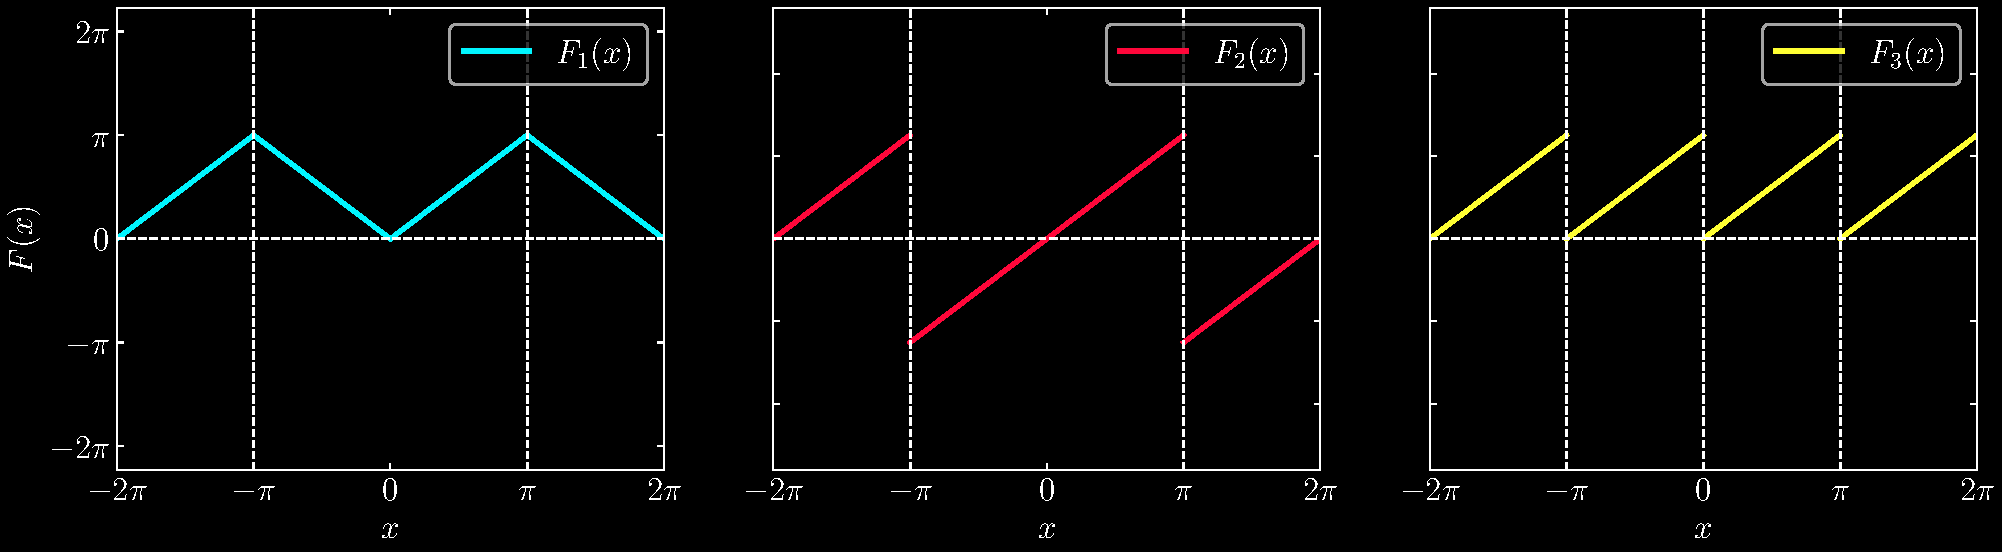
\includegraphics[width=1.0\textwidth]{../chap8/sec8.1/chap8sec8.1ex2.pdf}
\end{center}

% QUESTION 3
\qs{8.1.3}{Find the Fourier series on \( -\pi \le x \le \pi \)  for 
\begin{enumerate}[label=(\alph*)]
	\item \( f_{1}\!\left( x \right) = \sin^{3}\!\left(x\right) \), an odd function (sine series, only two terms)
	\item \( f_{2}\!\left( x \right) = \abs{\sin\!\left(x\right) } \), an even function (cosine series)
	\item \( f_{3}\!\left( x \right) = x \) for \( -\pi \le x \le \pi \) (sine series with jump at \( x = \pi \))
\end{enumerate}}

\begin{enumerate}[label=(\alph*)]
	\item The Fourier coefficients are given by
	\[
		b_{k} = \frac{2}{\pi} \int^{\pi}_{-\pi} \sin^{3}\!\left(x\right) \sin\!\left(kx\right) \, dx  
	\]
	The simplest approach is to write the identity \( \sin\!\left(x\right) = \!\left( e^{ix} - e^{-ix} \right) / 2i \). Then we can calculate
	\begin{align*}
		\sin^{3}\!\left(x\right) & = -\frac{1}{8i} \!\left( e^{ix} - e^{-ix} \right)^{3} \\
	                                 & = -\frac{1}{8i} \!\left( e^{3ix} - e^{-3ix} - 3 \!\left( e^{ix} - e^{-ix} \right) \right) \\ 
					 & = -\frac{1}{4} \!\left( \sin\!\left(3x\right) - 3 \sin\!\left(x\right) \right)
	\end{align*}
	which is a trigonometric identity that itself is also the Fourier series for \( \sin^{3}\!\left(x\right) \), and therefore \( b_{1} = 3/4 \) and \( b_{2} = -1/4 \).
	\item Note that the absolute value means
	\[
		\abs{\sin\!\left(x\right)} = \begin{cases}
			\sin\!\left(x\right) & 0 \le x \le \pi \\
			-\sin\!\left(x\right) & -\pi \le x < 0 \\
		\end{cases} 
	\]
	So calculating \( a_{0} \) yields
	\[
		a_{0} = \frac{1}{2 \pi} \!\left[ \int^{\pi}_{0} \sin\!\left(x\right) \, dx + \int^{0}_{-\pi} \!\left( -\sin\!\left(x\right) \right) \, dx \right] = \frac{2}{\pi}
	\]
	Deriving the Fourier coefficients, we find
	\begin{align*}
		a_{k} & = \frac{2}{\pi} \int^{\pi}_{0} \sin\!\left(x\right) \cos\!\left(kx\right) \, dx \\
		 & = -\frac{1}{\pi} \!\left[ \frac{\cos\!\left(1 - k\right) x}{1 - k} + \frac{\cos\!\left(1 + k\right) x}{1 + k} \right] \Big|^{\pi}_{0} \\
		 & = -\frac{1}{\pi \!\left( k^{2} - 1 \right)} \!\left[ \!\left( 1 + k \right)\cos\!\left(1 - k\right)x + \!\left( 1 - k \right)\cos\!\left(1 + k\right)x \right] \Big|^{\pi}_{0} 
	\end{align*}
	Now, when \( k \) is odd, this expression vanishes. Otherwise, for even \( k \) it reduces to
	\begin{align*}
		 & = \frac{1}{\pi \!\left( k^{2} - 1 \right)} \!\left[ -2 \!\left( 1 + k \right) - 2 \!\left( 1 - k \right) \right] \\
		 & = \frac{4}{\pi \!\left( 1 - k^{2} \right)}
	\end{align*}
	To cleanly put this in a summation, let \( k = 2n \). Then 
	\[
		\abs{\sin\!\left(x\right) } = \frac{2}{\pi} + \frac{4}{\pi} \sum_{n = 1}^{\infty} \frac{\cos\!\left(2nx\right) }{1 - 4n^{2}}, \quad -\pi \le x \le \pi
	\]
	\item The Fourier coefficients are
	\begin{align*}
		b_{k} & = \frac{1}{\pi} \int^{\pi}_{-\pi} x \sin\!\left(kx\right) \, dx \\
		 & = \frac{1}{\pi} \!\left[ \frac{\sin\!\left(kx\right) }{k^{2}} - \frac{x \cos\!\left(kx\right) }{k} \right] \Big|^{\pi}_{-\pi} 
	\end{align*}
	which is \( 2 / k \) when \( k \) is odd and \( -2 / k \) when \( k \) is even. By symmetry, \( b_{0} = 0 \). The Fourier sine series is
	\[
		x = 2 \sum_{n = 1}^{\infty} \frac{\!\left( -1 \right)^{n + 1}}{n} \sin\!\left(nx\right)  
	\]
\end{enumerate}

% QUESTION 4
\qs{8.1.4}{Find the complex Fourier series \( e^{x } = \sum c_{k} e^{ikx} \) on the interval \( -\pi \le x \le \pi \). The even part of a function is \( \frac{1}{2}\!\left( f \!\left( x \right) + f \!\left( -x \right) \right) \), so that \( f_{\text{even}}\!\left( x \right) = f_{\text{even}}\!\left( -x \right) \). Find the cosine series for \( f_{\text{even}} \) and the sine series for \( f_{\text{odd}} \). \textit{Notice the jump at }\( x = \pi \).}

First, we calculate the coefficients to the complex Fourier series as 
\begin{align*}
	c_{k} & = \frac{1}{2 \pi} \int^{\pi}_{-\pi} e^{x} e^{-ikx} \, dx \\
	 & = \frac{1}{2 \pi} \int^{\pi}_{-\pi} e^{\!\left( 1 - ik \right)x} \, dx  \\ 
	 & = \frac{1}{2 \pi} \frac{e^{\!\left( 1 - ik \right)x}}{1 - ik} \Big|^{\pi}_{-\pi} \\
	 & = \frac{1}{2 \pi \!\left( 1 - ik \right)} \!\left[ e^{\!\left( 1 - ik \right)\pi} - e^{-\!\left( 1 - ik \right)\pi} \right]
\end{align*}

Next, decompose the exponential function into the well-known identity
\[
	e^{x} = \underbrace{\frac{1}{2} \!\left( e^{x} + e^{-x} \right)}_{\text{even}} + \underbrace{\frac{1}{2} \!\left( e^{x} - e^{-x} \right)}_{\text{odd}} = \cosh\!\left( x \right) + \sinh\!\left( x \right)
\]

The Fourier cosine series for the even component is

\begin{align*}
	a_{k} & = \int^{\pi}_{-\pi} \frac{1}{2} \!\left( e^{x} + e^{-x} \right) \cos\!\left(kx\right) \, dx \\
	 & = \frac{2}{\pi} \int^{\pi}_{0} \frac{1}{2} \!\left( e^{x} + e^{-x} \right) \cos\!\left(kx\right) \, dx \\ 
	 & = \frac{1}{\pi} \!\left[ \frac{e^{x} \!\left( \cos\!\left(kx\right) + k \sin\!\left(kx\right)  \right)}{1 + k^{2}} + \frac{e^{-x} \!\left( -\cos\!\left(kx\right) + k \sin\!\left(kx\right)  \right)}{1 + k^{2}} \right] \Big|^{\pi}_{0} \\
	 & = \frac{\!\left( -1 \right)^{k}}{\pi} \!\left( \frac{e^{\pi} - e^{-\pi}}{1 + k^{2}} \right) \\
	 & = \!\left( -1 \right)^{k} \frac{2}{\pi \!\left( 1 + k^{2} \right)} \sinh\!\left( \pi \right)
\end{align*}

And for the Fourier sine series for the odd component, we have

\begin{align*}
	b_{k} & = \frac{1}{\pi} \int^{\pi}_{-\pi} \frac{1}{2} \!\left( e^{x} - e^{-x} \right) \sin\!\left(kx\right) \, dx \\
	 & = \frac{2}{\pi} \int^{\pi}_{0} \frac{1}{2} \!\left( e^{x} - e^{-x} \right) \sin\!\left(kx\right) \, dx \\ 
	 & = \frac{1}{\pi} \!\left[ \frac{e^{x} \!\left( \sin\!\left(kx\right) - k \cos\!\left(kx\right) \right)}{1 + k^{2}} - \frac{e^{-x} \!\left( -\sin\!\left(kx\right) - k \cos\!\left(kx\right) \right)}{1 + k^{2}} \right] \Big|^{\pi}_{0} \\
	 & = \!\left( -1 \right)^{k + 1} \frac{k}{\pi} \!\left( \frac{e^{\pi} - e^{-\pi}}{1 + k^{2}} \right) \\
	 & = \!\left( -1 \right)^{k + 1} \frac{2k}{\pi \!\left( 1 + k^{2} \right)} \sinh\!\left(\pi\right) 
\end{align*}

Additionally, the average is
\[
	a_{0} = \frac{1}{2 \pi} \int^{\pi}_{-\pi} e^{x} \, dx = \frac{1}{2 \pi} \!\left( e^{\pi} - e^{-\pi} \right) = \frac{1}{\pi} \sinh\!\left(\pi\right)   
\]
The full Fourier series for our \( F \!\left( x \right) \) is then
\[
	e^{x} = \frac{1}{\pi} \sinh\!\left(\pi\right) + \sum_{k = 1}^{\infty} \!\left( -1 \right)^{k} \frac{2}{\pi \!\left( 1 + k^{2} \right)} \sinh\!\left(\pi\right) \cos\!\left(kx\right) - \sum_{k = 1}^{\infty} \!\left( -1 \right)^{k} \frac{2k}{\pi \!\left( 1 + k^{2} \right)} \sinh\!\left(\pi\right) \sin\!\left(kx\right)  
\]

% QUESTION 5
\qs{8.1.5}{From the energy formula (21), the square wave sine coefficients satisfy
\[
	\pi \!\left( b_{1}^{2} + b_{2}^{2} + \cdots \right) = \int^{\pi}_{-\pi} \abs{SW \!\left( x \right)}^{2} \, dx = \int^{\pi}_{-\pi} 1 \, dx = 2 \pi
\]
Substitute the numbers \( b_{k} \) from equation (8) to find that \( \pi^{2} = 8 \!\left( 1 + \frac{1}{9} + \frac{1}{25} + \cdots \right) \).}	

The coefficients \( b_{k} \) are
\[
	b_{k} = \frac{2}{\pi} \!\left\{ \frac{2}{1}, \frac{2}{3}, \frac{2}{5}, \cdots \right\} 
\]
Substituting gives us
\[
	16 \pi \!\left( \frac{1}{\pi^{2}} + \frac{1}{9 \pi^{2}} + \frac{1}{25 \pi^{2}} + \cdots \right) = 2 \pi \quad \implies \quad \pi^{2} = 8 \!\left( 1 + \frac{1}{9} + \frac{1}{25} + \cdots \right)
\]

% QUESTION 6
\qs{8.1.6}{If a square pulse is centered at \( x = 0 \) to give
\[
	f \!\left( x \right) = 1 \quad \text{for} \quad \abs{x} < \frac{\pi}{2}, \quad f \!\left( x \right) = 0 \quad \text{for} \quad \frac{\pi}{2} < \abs{x} < \pi, 
\]
draw its graph and find its Fourier coefficients \( a_{k} \) and \( b_{k} \).}

\begin{center}
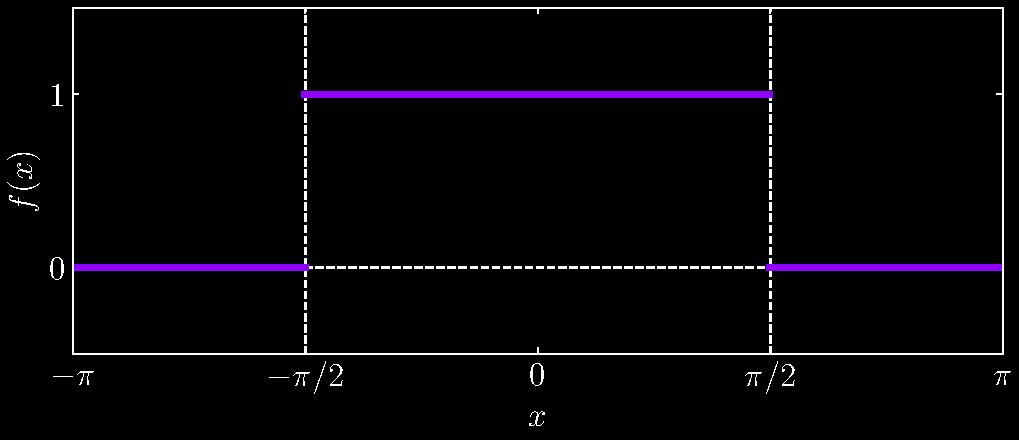
\includegraphics[width=1.0\textwidth]{../chap8/sec8.1/chap8sec8.1ex6.pdf}
\end{center}

On visual inspection, it is apparent that \( f \!\left( x \right) \) is an even function. From that we can immediately conclude that all \( b_{k} = 0 \). Then we calculate
\[
	a_{0} = \frac{1}{2 \pi} \int^{\pi}_{-\pi} f \!\left( x \right) \, dx = \frac{1}{2 \pi} \int^{\pi / 2}_{-\pi / 2}  \, dx = \frac{1}{2} 
\]
\begin{align*}
	a_{k} & = \frac{1}{\pi} \int^{\pi}_{-\pi} f \!\left( x \right) \cos\!\left(kx\right)  \, dx \\
	 & = \frac{1}{\pi} \int^{\pi / 2}_{-\pi / 2} \cos\!\left(kx\right) \, dx \\
	 & = \frac{2}{k \pi} \sin\!\left(\frac{k \pi}{2}\right)
\end{align*}
giving us complete Fourier series
\[
	f \!\left( x \right) = \frac{1}{2} + \sum_{k = 1}^{\infty} \frac{2}{k \pi} \sin\!\left(\frac{k \pi}{2}\right) \cos\!\left(kx\right)  
\]

% QUESTION 7
\qs{8.1.7}{Plot the first three partial sums and the function \( x \!\left( \pi - x \right) \):
\[
	x \!\left( \pi - x \right) = \frac{8}{\pi} \!\left( \frac{\sin\!\left(x\right) }{1} + \frac{\sin\!\left(3x\right) }{27} + \frac{\sin\!\left(5x\right) }{125} + \cdots \right), \quad 0 < x < \pi 
\]
Why is \( 1 / k^{3} \) the decay rate for this function? What is its second derivative?}

\begin{center}
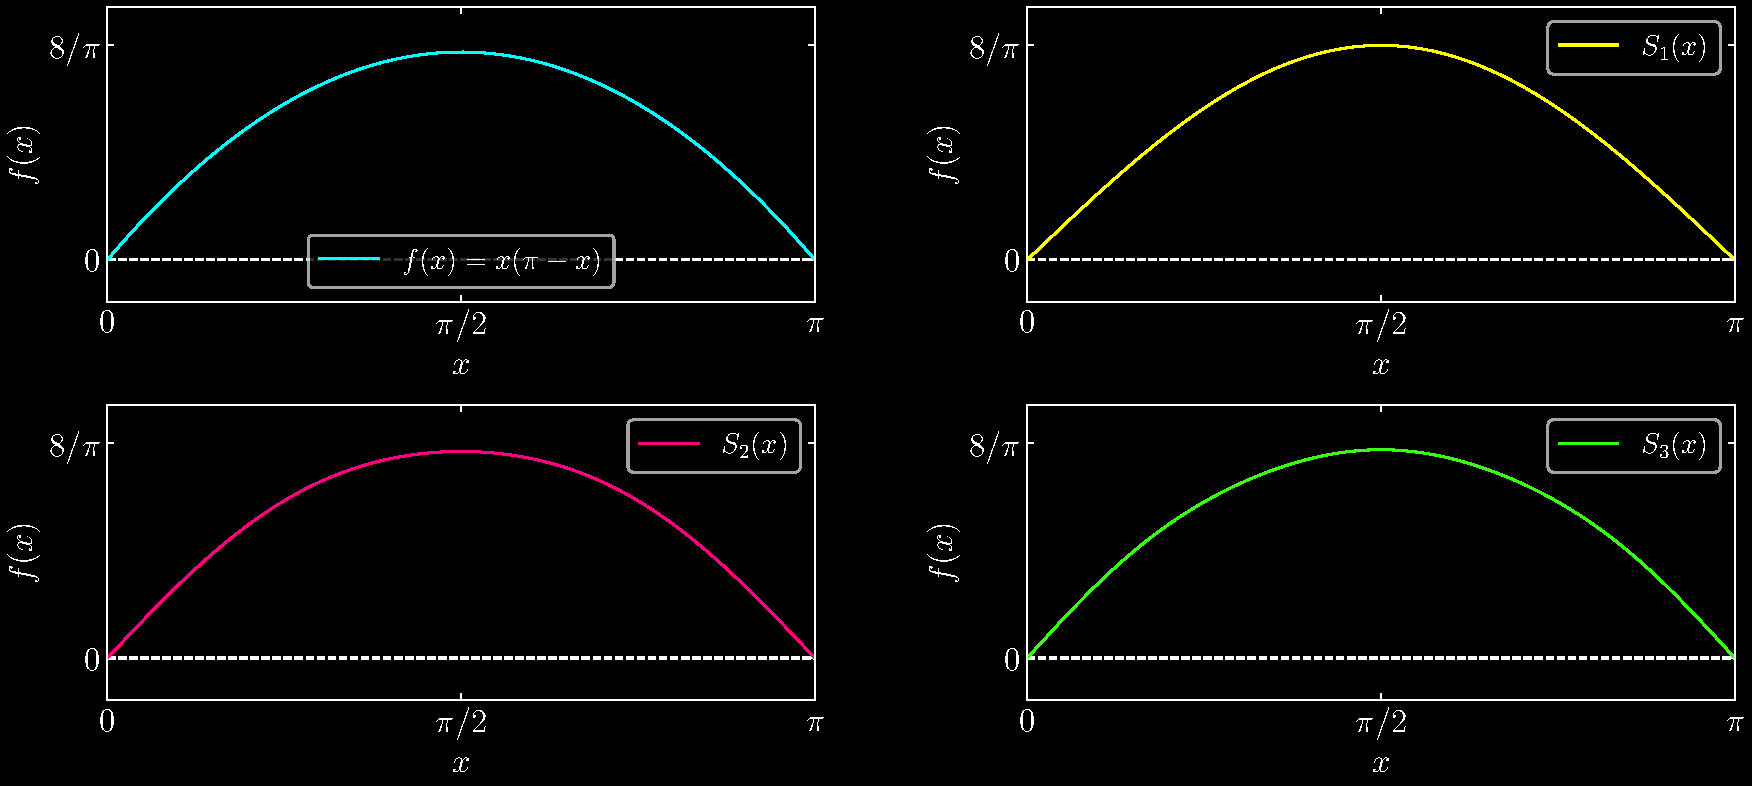
\includegraphics[width=1.0\textwidth]{../chap8/sec8.1/chap8sec8.1ex7.pdf}
\end{center}

The second derivative is \( f'' = -2 \). One analysis here is we must integrate thrice to derive our Fourier coefficient: twice for the \( x^{2} \) term, and once more for the sine. This generates \( 1 / k^{3} \).

Another way to think about the decay rate is as follows: \( 1/k \) corresponds to jumps in the function itself (step functions), \( 1/k^{2} \) is the jump in the first derivative of the ramp function, and \( 1/k^{3} \) for the jump in the second derivative. The argument here, then, requires us to consider the periodic odd extension of \( f \), namely the case where
\[
	f = x \pi + x^{2}, \quad -\pi < x < 0
\]
In this ``branch'', the second derivative is \( +2 \). At \( x = 0 \), we have a discontinuity in the second derivative: the jump from \( +2 \) to \( -2 \).

\vspace{12pt}

% QUESTION 8
\qs{8.1.8}{Sketch the \( 2 \pi \)-periodic half wave with \( f \!\left( x \right) = \sin\!\left(x\right) \) for \( 0 < x < \pi \) and \( f \!\left( x \right) = 0 \) for \( -\pi < x < 0 \). Find its Fourier series.}

\begin{center}
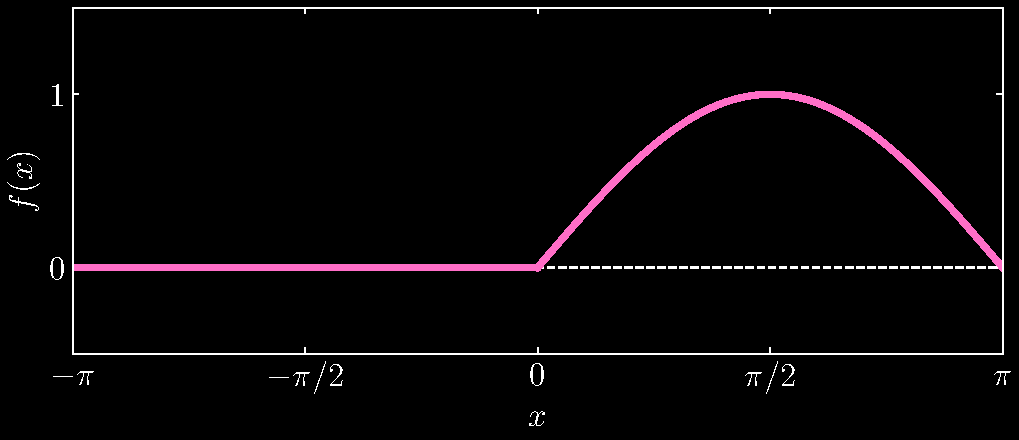
\includegraphics[width=1.0\textwidth]{../chap8/sec8.1/chap8sec8.1ex8.pdf}
\end{center}

The Fourier series is calculated as 
\begin{align*}
	a_{0} & = \frac{1}{2 \pi} \int^{\pi}_{-\pi} f \!\left( x \right) \, dx \\
	 & = \frac{1}{2 \pi} \int^{\pi}_{0} \sin\!\left(x\right) \, dx \\ 
	 & = \frac{1}{\pi} \\
	a_{k} & = \frac{1}{\pi} \int^{\pi}_{0} \sin\!\left(x\right) \cos\!\left(kx\right) \, dx \\
	      & = \frac{1}{\pi} \!\left[ -\frac{\cos\!\left(\!\left( 1 - k \right)x\right) }{2 \!\left( 1 - k \right)} - \frac{\cos\!\left(\!\left( 1 + k \right)x\right) }{2 \!\left( 1 + k \right)} \right] \Big|^{\pi}_{0} \\
	      & = \frac{1}{\pi} \!\left[ \frac{\cos\!\left(k \pi\right) + 1}{2 \!\left( 1 - k \right)} + \frac{\cos\!\left(k \pi\right) + 1}{2 \!\left( 1 + k \right)} \right] \\
\implies a_{n} & = \frac{1}{\pi} \!\left[ \frac{1}{1 - 2n} + \frac{1}{1 + 2n} \right] \quad (\text{substitute } k = 2n \text{; non-zero only for even } k) \\
	      & = \frac{2}{\pi \!\left( 1 - 4n^{2} \right)} \\
	b_{k} & = \frac{1}{\pi} \int^{\pi}_{0} \sin\!\left(x\right) \sin\!\left(kx\right) \, dx \\
	      & = \frac{1}{\pi}\!\left[ \frac{x}{2} - \frac{\sin\!\left(2x\right) }{4} \right] \Big|^{\pi}_{0} \\
	      & = \frac{1}{2}
\end{align*}
which gives us
\[
	f \!\left( x \right) = \frac{1}{\pi} + \sum_{n = 1}^{\infty} \frac{2}{\pi \!\left( 1 - 4n^{2} \right)} + \frac{\sin\!\left(x\right) }{2} 
\]

% QUESTION 9
\qs{8.1.9}{Suppose \( G \!\left( x \right) \) has period \( 2L \) instead of \( 2 \pi \). Then \( G \!\left( x + 2L \right) = G \!\left( x \right) \). Integrals go from \( -L \) to \( L \) or from \( 0 \) to \( 2L \). The Fourier formulas change by a factor \( \pi / L \):

The coefficients in 

\( G \!\left( x \right) = \sum_{-\infty}^{\infty} \pmb{C}_{k} e^{ik \pi x / L} \) are \( \displaystyle{\pmb{C}_{k} = \frac{1}{2L} \int^{L}_{-L} G \!\left( x \right) e^{-ik \pi x / L} \, dx } \).

Derive this formula for \( C_{k} \): Multiply the first equation for \( G \!\left( x \right) \) by \underline{\qquad} and integrate both sides. Why is the integral on the right side equal to \( 2LC_{k} \)?}

Multiply the first equation by \( e^{-ik \pi x / L} \). 
\[
	G \!\left( x \right) e^{-ik \pi x / L} = e^{-ik \pi x / L} \sum_{-\infty}^{\infty} C_{k} e^{ik \pi x / L} 
\]
By orthogonality of the complex exponentials, after integrating, we are left only with 
\[
	\int^{L}_{-L} G \!\left( x \right) e^{-ik \pi x / L} \, dx = \int^{L}_{-L} C_{k} \, dx = 2LC_{k} 
\]

% QUESTION 10
\qs{8.1.10}{For \( G_{\text{even}} \), use Problem 9 to find the cosine coefficient \( A_{k} \) from \( \!\left( C_{k} + C_{-k} \right) / 2 \):
\[
	G_{\text{even}}\!\left( x \right) = \sum_{0}^{\infty} A_{k} \cos\!\left(\frac{k \pi x }{L}\right) \text{ has } A_{k} = \frac{1}{L} \int^{L}_{0} G_{\text{even}}\!\left( x \right) \cos\!\left(\frac{k \pi x}{L}\right) \, dx.  
\]
\( G_{\text{even}} \) is \( \frac{1}{2} \!\left( G \!\left( x \right) + G \!\left( -x \right) \right) \). Exception for \( A_{0} = C_{0} \): Divide by \( 2L \) instead of \( L \).}

Calculate
\begin{align*}
	\frac{c_{k} + c_{-k}}{2} & = \frac{1}{4L} \!\left[ \int^{L}_{-L} G \!\left( x \right) e^{-ik \pi x / L} \, dx + \int^{L}_{-L} G \!\left( x \right) e^{i k \pi x / L} \, dx \right] \\
	 & = \frac{1}{2L} \int^{L}_{-L} G \!\left( x \right) \cos\!\left(\frac{k \pi x }{L}\right) \, dx \\ 
	 & = \frac{1}{2L} \int^{L}_{-L} \!\left[ \underbrace{\frac{1}{2} \!\left( G \!\left( x \right) + G \!\left( -x \right) \right)}_{\text{even}} + \underbrace{\frac{1}{2} \!\left( G \!\left( x \right) - G \!\left( -x \right) \right)}_{\text{odd}} \right] \cos\!\left(\frac{k \pi x }{L}\right) \, dx \\ 
	 & = \frac{1}{2L} \int^{L}_{-L} G_{\text{even}}\!\left( x \right) \cos\!\left(\frac{k \pi x }{L}\right)  \, dx \\
	 & = \frac{1}{L} \int^{L}_{0} G_{\text{even}}\!\left( x \right) \cos\!\left(\frac{k \pi x }{L}\right) \, dx \\
	 & = A_{k}
\end{align*}

Recall that in the third line, since an odd function times an even function is odd, the second integral vanishes over the symmetric bounds. This leaves only the even component of \( G \!\left( x \right) \).

\vspace{12pt}

% QUESTION 11
\qs{8.1.11}{Problem 10 tells us that \( \displaystyle{\pmb{a_{k} = \frac{1}{2} \!\left( c_{k} + c_{-k} \right)}} \) on the usual interval from \( 0 \) to \( \pi \). Find a similar formula for \( b_{k} \) from \( c_{k} \) and \( c_{-k} \). In the reverse direction, find the complex coefficient \( c_{k} \) in \( F \!\left( x \right) = \sum c_{k}e^{ikx} \) from the real coefficients \( a_{k} \) and \( b_{k} \).}

A point of clarification is warranted. Problem 8.1.10 calculates the Fourier coefficient for the \textit{even extension of} \( G \!\left( x \right) \). We can do the same for the \textit{odd} extension of \( G \!\left( x \right) \), which involves reworking the derivation in the previous problem to ensure that the sine term survives. The way to do so is to begin from \( \!\left( c_{k} - c_{-k} \right) / 2 \). Doing so leaves us with
\[
	\frac{c_{k} - c_{-k}}{2} = -\frac{i}{2L} \int^{L}_{-L} G_{\text{odd}}\!\left( x \right)\sin\!\left(\frac{k \pi x }{L}\right) \, dx
\]
Multiply by \( i \) to conclude
\[
	i \!\left( \frac{c_{k} - c_{-k}}{2} \right) = \frac{1}{2L} \int^{L}_{-L} G_{\text{odd}}\!\left( x \right) \sin\!\left(\frac{k \pi x }{L}\right) \, dx = B_{k}
\]
Now, we consider the original function \( G \!\left( x \right) \) (with the definition in Problem 8.1.9). Fix \( k \) and write
\begin{align*}
	c_{k} & = \frac{1}{2L} \int^{L}_{-L} G \!\left( x \right) e^{-ik \pi x / L} \, dx \\
	 & = \frac{1}{2L} \int^{L}_{-L} G \!\left( x \right) \!\left[ \cos\!\left(\frac{k \pi x}{L}\right) - i \sin\!\left(\frac{k \pi x}{L}\right) \right] \, dx \\ 
	 & = \frac{1}{2} \!\left( a_{k} - i b_{k} \right)
\end{align*}
Analogously conclude that
\[
	c_{-k} = \frac{1}{2} \!\left( a_{k} + i b_{k} \right) 
\]
Two equations for two unknowns gives us
\begin{align*}
	a_{k} & = c_{k} + c_{-k} \\
	b_{k} & = i \!\left( c_{k} - c_{-k} \right)
\end{align*}
which are the great and elegant formulae for relating the complex and trigonometric Fourier coefficients for \( G \!\left( x \right) \).

\vspace{12pt}

% QUESTION 12
\qs{8.1.12}{Find the solution to Laplace's equation with \( u_{0} = \theta \) on the boundary. Why is this the imaginary part of \( 2 \!\left( z - z^{2} / 2 + z^{3} / 3 \cdots \right) = 2 \log\!\left( 1 + z \right) \)? Confirm that on the unit circle \( z = e^{i \theta} \), the imaginary part of \( 2 \log\!\left( 1 + z \right) \) agrees with \( \theta \).}

Since \( u_{0} \!\left( \theta \right) = \theta \) is an odd function, we calculate the sine series as 
\begin{align*}
	b_{0} & = \frac{1}{\pi} \int^{\pi}_{-\pi} \theta \, d \theta \\
	 & = 0 \\ 
	b_{k} & = \frac{1}{\pi} \int^{\pi}_{-\pi} \theta \sin\!\left(k \theta\right) \, d \theta \\
	      & = \frac{1}{\pi} \!\left[ \frac{\sin\!\left(k \theta\right)}{k^{2}} - \frac{\theta \cos\!\left(k \theta\right)}{k} \right] \Big|^{\pi}_{-\pi} \\
	      & = \frac{2}{k}\!\left( -1 \right)^{k + 1}
\end{align*}

The solution to Laplace's equation is
\[
	u\!\left( r, \theta \right) = \frac{2}{1}r \sin\!\left(\theta\right) - \frac{2}{2}r^{2}\sin\!\left(2 \theta\right) + \frac{2}{3}r^{3}\sin\!\left(3 \theta\right) - \cdots = \sum_{k = 1}^{\infty} \frac{2}{k}\!\left( -1 \right)^{k + 1}r^{k} \sin\!\left(k \theta\right)  
\]
Let \( z = re^{i \theta} \). Then this solution indeed corresponds to \( \Imag \!\left[ 2 \log \!\left( 1 + z \right) \right] \).

\vspace{12pt}

% QUESTION 13
\qs{8.1.13}{If the boundary condition for Laplace's equation is \( u_{0} = 1 \) for \( 0 < \theta < \pi \) and \( u_{0} = 0 \) for \( -\pi < \theta < 0 \), find the Fourier series solution \( u \!\left( r, \theta \right) \) inside the unit circle. What is \( u \) at the origin \( r = 0 \)?}

We must calculate the complete Fourier series, which is
\begin{align*}
	a_{0} & = \frac{1}{2 \pi} \int^{\pi}_{-\pi} u_{0} \, d \theta \\
	 & = \frac{1}{2 \pi} \int^{\pi}_{0} \, d \theta \\ 
	 & = \frac{1}{2} \\
	a_{k} & = \frac{1}{\pi} \int^{\pi}_{0} \cos\!\left(k \theta\right) \, d \theta \\
	      & = 0 \\
	b_{k} & = \frac{1}{\pi} \int^{\pi}_{0} \sin\!\left(k \theta\right) \, d \theta \\
	      & = \frac{1}{\pi} \!\left[ \frac{\!\left( -1 \right)^{k + 1} + 1}{k} \right]
\end{align*}
This vanishes for even \( k \), so we should write
\[
	b_{n} = \frac{2}{\pi \!\left( 2n - 1 \right)} 
\]
The solution to Laplace's equation is
\[
	u \!\left( r, \theta \right) = \frac{1}{2} + \sum_{n = 1}^{\infty} \frac{2}{\pi \!\left( 2n - 1 \right)} r^{2n - 1} \sin\!\left(\!\left( 2n - 1 \right) \theta \right)
\]

% QUESTION 14
\qs{8.1.14}{With boundary values \( u_{0}\!\left( \theta \right) = 1 + \frac{1}{2}e^{i \theta} + \frac{1}{4}e^{2i \theta} + \cdots \), what is the Fourier series solution to Laplace's equation in the circle? Sum this geometric series.}

Multiply each term by the corresponding power of \( r \) to get
\[
	u \!\left( r, \theta \right) = \sum_{n = 0}^{\infty} \!\left( \frac{1}{2}re^{i \theta} \right)^{n}
\]
For this infinite sum, we have closed-form expression
\[
	u \!\left( r, \theta \right) = \frac{1}{1 - \frac{1}{2}re^{i \theta}}
\]

% QUESTION 15
\qs{8.1.15}{
\begin{enumerate}[label=(\alph*)]
	\item Verify that the fraction in Poisson's formula (30) satisfies Laplace's equation.
	\item Find the response \( u \!\left( r, \theta \right) \) to an impulse at \( x = 0 \), \( y = 1 \) (where \( \theta = \frac{\pi}{2} \)).
\end{enumerate}}

\begin{enumerate}[label=(\alph*)]
	\item In \( \!\left( r, \theta \right) \) coordinates, Laplace's equation is
	\[
		\frac{\partial^{2} u}{\partial r^{2}} + \frac{1}{r} \frac{\partial u}{\partial r} + \frac{1}{r^{2}} \frac{\partial^{2} u}{\partial \theta^{2}} = 0
	\]
	Note that the Poisson's equation has, for the purposes of differentiation, a more legible summation form
	\[
		u \!\left( r, \theta \right) = \frac{1}{2 \pi} + \frac{1}{\pi} \sum_{n = 1}^{\infty} r^{n}\cos\!\left(n \theta\right) 
	\]
	Each term is calculated as 
	\begin{align*}
		\frac{\partial^{2} u}{\partial r^{2}} & = \frac{1}{\pi} \sum_{n = 1}^{\infty} n \!\left( n - 1 \right) r^{n - 2} \cos\!\left(n \theta\right) \\
		\frac{1}{r} \frac{\partial u}{\partial r} & = \frac{1}{\pi} \sum_{n = 1}^{\infty} nr^{n - 2} \cos\!\left(n \theta\right) \\
		\frac{1}{r^{2}} \frac{\partial^{2} u}{\partial \theta^{2}} & = -\frac{1}{\pi} \sum_{n = 1}^{\infty} n^{2}r^{n - 2} \cos\!\left(n \theta\right) 
	\end{align*}
	which, expectedly, vanish upon summation.
	\item Think of the impulse as undergoing an angular displacement of \( \theta = \pi / 2 \). The phase shift \( \cos\!\left(\theta + \pi / 2 \right) \) becomes \( -\sin\!\left(\theta\right) \). Poisson's equation becomes
	\[
		u \!\left( r, \theta \right) = \frac{1}{2 \pi} \frac{1 - r^{2}}{1 + r^{2} + 2r \sin\!\left(\theta\right) } 
	\]
\end{enumerate}

% QUESTION 16
\qs{8.1.16}{With complex exponentials in \( F \!\left( x \right) = \sum c_{k}e^{ikx} \), the energy identity (21) changes to \( \int^{\pi}_{-\pi} \abs{F \!\left( x \right)}^{2} \, dx = 2 \pi \sum \abs{c_{k}}^{2} \). Derive this by integrating \( \!\left( \sum c_{k}e^{ikx} \right)\!\left( \sum \overline{c}_{k}e^{-ikx} \right) \).}

By orthogonality, we know that surviving terms will only be those with the same \( k \) in both summations. This leaves us with
\[
	\int^{\pi}_{-\pi} \sum \abs{c_{k}}^{2} \, dx = 2 \pi \sum \abs{c_{k}}^{2} 
\]

% QUESTION 17
\qs{8.1.17}{A centered square wave has \( F \!\left( x \right) = 1 \) for \( \abs{x} \le \pi / 2 \).
\begin{enumerate}[label=(\alph*)]
	\item Find its energy \( \int \abs{F \!\left( x \right)}^{2} \, dx \) by direct integration
	\item Compute its Fourier coefficients \( c_{k} \) as specific numbers
	\item Find the sum in the energy identity (Problem 16).
\end{enumerate}}

\begin{enumerate}[label=(\alph*)]
	\item 
	\[
		\int^{\pi}_{-\pi} \abs{F \!\left( x \right)}^{2} \, dx = \int^{\pi / 2}_{-\pi / 2} \, dx = \pi   
	\]
	\item 
	\begin{align*}
		c_{k} & = \frac{1}{2 \pi} \int^{\pi / 2}_{-\pi / 2} e^{-ikx} \, dx \\ 
		      & = -\frac{1}{2 \pi ik} \!\left( e^{-ik \pi / 2} - e^{i k \pi / 2} \right) \\ 
		      & = \frac{1}{\pi k} \sin\!\left(\frac{k \pi}{2}\right)
	\end{align*}
	In general, the squared coefficients take on form
	\[
		\abs{c_{k}}^{2} = 
		\begin{cases}
			\displaystyle{\frac{1}{4}}, & k = 0 \\
			\displaystyle{\frac{1}{\pi^{2} \!\left( 2k - 1 \right)^{2}}}, & k > 0
		\end{cases}
	\]
	\item 
	Since we need to sum over all integers (positive, negative, and zero), we need to multiply the summation here by two to account for the negatives (as it only sums from \( k = 1 \) onward), and add \( \abs{c_{0}^{2}} \).
	\begin{align*}
		\int^{\pi}_{-\pi} \sum \abs{c_{k}}^{2} \, dx & = 2 \pi \sum_{-\infty}^{\infty}  \abs{c_{k}}^{2} \\
										& = 2 \pi \!\left( \abs{c_{0}}^{2} + \sum_{k = 1}^{\infty} \!\left( \abs{c_{k}}^{2} + \abs{c_{-k}}^{2} \right) \right) \\
										& = 2 \pi \!\left( \abs{c_{0}}^{2} + 2 \sum_{k = 1}^{\infty} \abs{c_{k}}^{2} \right) \\
		 & = 2 \pi \!\left( \frac{1}{4} + 2 \sum \frac{1}{\pi^{2} \!\left( 2k - 1 \right)^{2}} \right) \\ 
		 & = 2 \pi \!\left( \frac{1}{4} + \frac{1}{4} \right) \\
		 & = \pi
	\end{align*}
\end{enumerate}

% QUESTION 18
\qs{8.1.18}{\( F \!\left( x \right) = 1 + \!\left( \cos\!\left(x\right) \right) / 2 + \cdots + \!\left( \cos\!\left(nx\right) \right) / 2^{n} + \cdots \) is analytic: infinitely smooth.
\begin{enumerate}[label=(\alph*)]
	\item If you take 10 derivatives, what is the Fourier series of \( d^{10} F / dx^{10} \)?
	\item Does that series still converge quickly? Compare \( n^{10} \) with \( 2^{n} \) for \( n = 2^{10} \).
\end{enumerate}}

\begin{enumerate}[label=(\alph*)]
	\item We have
	\[
		F^{10}\!\left( x \right) = - \!\left[ \frac{\cos\!\left(x\right) }{2} + \cdots + \frac{n^{10}\cos\!\left(nx\right) }{2^{n}} + \cdots \right] = -\sum_{k = 1}^{\infty} \frac{k^{10}\cos\!\left(kx\right) }{2^{k}}
	\]
	which is indeed its own Fourier series.
	\item Yes; \( \!\left( 2^{10} \right)^{10} = 2^{100} \) is immensely less than \( 2^{2^{10}} \). In general, \( n^{10} \) grows much slower than \( 2^{n} \) for large \( n \).
\end{enumerate}

% QUESTION 19
\qs{8.1.19}{If \( f \!\left( x \right) = 1 \) for \( \abs{x} \le \pi / 2\) and \( f \!\left( x \right) = 0 \) for \( \pi / 2 < \abs{x} < \pi \), find its cosine coefficients. Can you graph and compute the Gibbs overshoot at the jumps?}

The cosine coefficients are
\[
	a_{k} = \frac{1}{\pi} \int^{\pi / 2}_{-\pi / 2} \cos\!\left(kx\right) \, dx = \frac{2}{\pi k} \sin\!\left(\frac{k \pi}{2}\right)
\]
which reduces to
\[
	a_{n} = \!\left( -1 \right)^{n + 1}\frac{2}{\pi \!\left( 2n - 1 \right)}
\]
Since \( a_{0} = 1/2 \), the Fourier cosine series is
\[
	f \!\left( x \right) = \frac{1}{2} + \sum_{n = 1}^{\infty} \!\left( -1 \right)^{n + 1}\frac{2}{\pi \!\left( 2n - 1 \right)} \cos\!\left(\!\left( 2n - 1 \right)x\right) 
\]

The Gibbs overshoot for numerous values of partial sums \( S_{N} \) is
\begin{center}
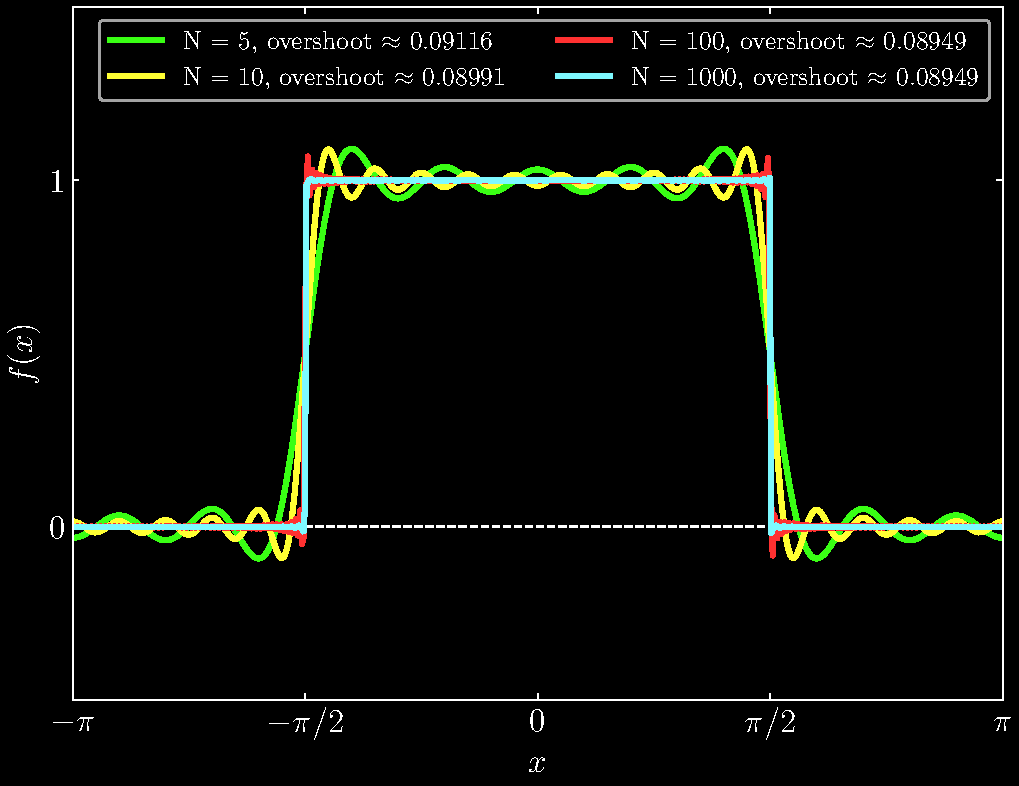
\includegraphics[width=1.0\textwidth]{../chap8/sec8.1/chap8sec8.1ex19.pdf}
\end{center}

\newpage
% QUESTION 20
\qs{8.1.20}{Find all the coefficients \( a_{k} \) and \( b_{k} \) for \( F \), \( I \), and \( D \) on the interval \( -\pi \le x \le \pi \):
\[
	F \!\left( x \right) = \delta \!\left( x - \frac{\pi}{2} \right) \quad I \!\left( x \right) = \int^{x}_{0} \delta \!\left( x - \frac{\pi}{2} \right) \, dx \quad D \!\left( x \right) = \frac{d }{d x} \delta \!\left( x - \frac{\pi}{2} \right)  
\]}

\( F \!\left( x \right) \):

\begin{align*}
	a_{0} & = \frac{1}{2 \pi} \int^{\pi}_{-\pi} \delta\!\left( x - \frac{\pi}{2} \right) \, dx \\ 
	a_{k} & = \frac{1}{\pi} \int^{\pi}_{-\pi} \cos\!\left(kx\right) \delta\!\left( x - \frac{\pi}{2} \right) \, dx \\
	 & = \frac{1}{\pi} \cos\!\left(\frac{k \pi}{2}\right) \\
	b_{k} & = \frac{1}{\pi} \int^{\pi}_{-\pi} \sin\!\left(kx\right) \delta\!\left( x - \frac{\pi}{2} \right) \, dx \\
	      & = \frac{1}{\pi} \sin\!\left(\frac{k \pi}{2}\right) 
\end{align*}

\( I \!\left( x \right) \): Note that this \( I \!\left( x \right) \) is a definition of the Heaviside step function \( \displaystyle{H \!\left( x - \frac{\pi}{2} \right)} \).

\begin{align*}
	a_{0} & = \frac{1}{2 \pi} \int^{\pi}_{-\pi} \int^{x}_{0} \delta\!\left( x - \frac{\pi}{2} \right) \, dx \, dx \\
	 & = \frac{1}{2 \pi} \int^{\pi}_{-\pi} H \!\left( x - \frac{\pi}{2} \right) \, dx \\ 
	 & = \frac{1}{4} \\
	a_{k} & = \frac{1}{\pi} \int^{\pi}_{-\pi} \cos\!\left(kx\right) H \!\left( x - \frac{\pi}{2} \right) \, dx \\
	      & = \frac{1}{\pi k} \!\left[ \sin\!\left(k \pi\right) - \sin\!\left(\frac{k \pi}{2}\right) \right] \\
	      & = -\frac{1}{\pi k} \sin\!\left(\frac{k \pi}{2}\right) \\
	b_{k} & = \frac{1}{\pi} \int^{\pi}_{-\pi} \sin\!\left(kx\right) H \!\left( x - \frac{\pi}{2} \right) \, dx \\
	      & = \frac{1}{\pi k} \!\left[ \cos\!\left(\frac{k \pi}{2}\right) - \cos\!\left(k \pi\right) \right]
\end{align*}

\( D \!\left( x \right) \): Relying on the intuition of integration by parts is key, although remember that the delta function is not a ``function'' in the rigorous sense (for reasons beyond our scope here).

For \( a_{0} \), let \( u = 1 \) and \( dv = \displaystyle{\frac{d }{d x} \delta\!\left( x - \frac{\pi}{2} \right)} \, dx \). Then \( du = 0 \) and \( v = \displaystyle{\delta\!\left( x - \frac{\pi}{2} \right)} \).
\begin{align*}
	a_{0} & = \frac{1}{2 \pi} \int^{\pi}_{-\pi} \frac{d }{d x} \delta \!\left( x - \frac{\pi}{2} \right) \, dx \\
	      & = \frac{1}{2 \pi} \delta \!\left( x - \frac{\pi}{2} \right) \Big|^{\pi}_{-\pi} \\ 
	      & = 0
\end{align*}
In the cases of \( a_{k} \) and \( b_{k} \), let \( u = \cos\!\left(kx\right) \) or \( u = \sin\!\left(kx\right) \), corresponding to \( du = -k \sin\!\left(kx\right) \) or \( du = k \cos\!\left(kx\right) \).
\begin{align*}
	a_{k} & = \frac{1}{2 \pi} \int^{\pi}_{-\pi} \cos\!\left(kx\right) \frac{d }{d x} \delta\!\left( x - \frac{\pi}{2} \right) \, dx \\
	 & = -\frac{k}{2 \pi} \int^{\pi}_{-\pi} \sin\!\left(kx\right) \delta\!\left( x - \frac{\pi}{2} \right) \, dx \\
	 & = -\frac{k}{2 \pi} \sin\!\left(\frac{k \pi}{2}\right) \\
	b_{k} & = \frac{1}{2 \pi} \int^{\pi}_{-\pi} \sin\!\left(kx\right) \frac{d }{d x} \delta\!\left( x - \frac{\pi}{2} \right) \, dx \\
	      & = \frac{k}{2 \pi} \int^{\pi}_{-\pi} \cos\!\left(kx\right) \delta\!\left( x - \frac{\pi}{2} \right) \, dx \\
	      & = \frac{k}{2 \pi} \cos\!\left(kx\right) 
\end{align*}
Observe that \( a_{k} \) and \( b_{k} \) here are the Fourier coefficients of the step functioncase multipled by \( k \).

\vspace{12pt}

% QUESTION 21
\qs{8.1.21}{For the one-sided tall box function in Example 4, with \( F = 1/h \) for \( 0 \le x \le h \), what is its odd part \( \frac{1}{2}\!\left( F \!\left( x \right) - F \!\left( -x \right) \right) \)? I am surprised that the Fourier coefficients of this odd part disappear as \( h \) approaches zero and \( F \!\left( x \right) \) approaches \( \delta\!\left( x \right) \).}

In order for the even and odd decomposition to work, we should clarify that our \( F \) is defined over a symmetric interval \( -h \le x \le h \), namely
\[
	F \!\left( x \right) = 
	\begin{cases}
		1 / h, & 0 \le x \le h \\
		0, & -h \le x < 0 \\
	\end{cases}
\]
Given the piecewise nature of this function, we must calculate the odd part on each interval. First, over \( 0 \le x \le h \):
\[
	F_{\text{odd}} = \frac{1}{2}\!\left( \frac{1}{h} - 0 \right) = \frac{1}{2h}
\]
and secondly, over \( -h \le x < 0 \):
\[
	F_{\text{odd}} = \frac{1}{2}\!\left( 0 - \frac{1}{h} \right) = -\frac{1}{2h} 
\]
Now we calculate the Fourier coefficients
\begin{align*}
	a_{0} & = \frac{1}{2 h} \int^{h}_{-h} F \!\left( x \right) \, dx \\
	 & = \frac{1}{2 h} \!\left[ \int^{h}_{0} \frac{1}{2h} \, dx - \int^{0}_{-h} \frac{1}{2h} \, dx \right] \\ 
	 & = \frac{1}{2 h} \!\left[ \frac{1}{2} - \frac{1}{2} \right] \\
	 & = 0 \\
	a_{k} & = \frac{1}{h} \int^{h}_{-h} F \!\left( x \right) \cos\!\left(kx\right) \, dx  \\
	 & = \frac{1}{2h^{2}} \!\left[ \int^{h}_{0} \cos\!\left(kx\right) \, dx - \int^{0}_{-h} \cos\!\left(kx\right) \, dx \right] \\
	 & = 0 \\
	b_{k} & = \frac{1}{\pi} \int^{h}_{-h} F \!\left( x \right)\sin\!\left(kx\right) \, dx \\
	 & = \frac{1}{2 \pi h} \!\left[ \int^{h}_{0} \sin\!\left(kx\right) \, dx - \int^{0}_{-h} \sin\!\left(kx\right) \, dx \right] \\
	 & = \frac{1}{2 \pi kh} \!\left[ -\cos\!\left(kh\right) + 1 + 1 - \cos\!\left(kh\right) \right] \\
	 & = \frac{\cos\!\left(kh\right) - 1}{\pi k h}
\end{align*}

In the limit, we can apply l'H\^{o}pital's rule to find that \( b_{k} \rightarrow 0 \) as \( h \rightarrow 0 \), though \( b_{k} \) is never truly zero.

\vspace{12pt}

% QUESTION 22
\qs{8.1.22}{Find the series \( F \!\left( x \right) = \sum c_{k}e^{ikx} \) for \( F \!\left( x \right) = e^{x} \) on \( -\pi \le x \le \pi \). That function \( e^{x} \) looks smooth, but there must be a hidden jump to get coefficients \( c_{k} \) proportional to \( 1 / k \). Where is the jump?}

The coefficients are
\begin{align*}
	c_{k} & = \frac{1}{2 \pi} \int^{\pi}_{-\pi} e^{x}e^{-ikx} \, dx \\
	 & = \frac{1}{2 \pi} \int^{\pi}_{-\pi} e^{\!\left( 1 - ik \right)x} \, dx \\
	 & = \frac{1}{2 \pi \!\left( 1 - ik \right)} e^{\!\left( 1 - ik \right)x} \Big|^{\pi}_{-\pi} \\
	 & = \frac{1}{2 \pi \!\left( 1 - ik \right)} \!\left[ e^{\!\left( 1 - ik \right)\pi } - e^{-\!\left( 1 - ik \right) \pi} \right] \\
	 & = \frac{\!\left( -1 \right)^{k}}{2 \pi \!\left( 1 - ik \right)} \!\left[ e^{\pi} - e^{-\pi} \right]
\end{align*}

The jumps occur at every \( x = \!\left( 2k + 1 \right)\pi \), where we go from \( e^{\pi} \) down to \( e^{-\pi} \). That jump appears as a factor in the Fourier coefficients.

\vspace{12pt}

% QUESTION 23
\qs{8.1.23}{\begin{enumerate}[label=(\alph*)]
	\item (Old particular solution) Solve \( Ay'' + By' + Cy = e^{ikx} \).
	\item (New particular solution) Solve \( Ay'' + By' + Cy = \sum c_{k}e^{ikx} \).
\end{enumerate}}

\begin{enumerate}[label=(\alph*)]
	\item Let \( y_{p} = Y_{k}e^{ikx} \). Then \( y'' = -k^{2}Y_{k}e^{ikx} \) and \( y' = ikY_{k}e^{ikx} \). We have
	\[
		-k^{2}Y_{k}A + ikY_{k}B + Y_{k}C = 1 \quad \implies \quad Y_{k} = \frac{1}{C - k^{2}A + ikB}
	\]
	\item By superposition,
	\[
		y_{p} = \sum c_{k}Y_{k}e^{ikx}
	\]
\end{enumerate}

\newpage
\subsection{\textsf{8.2 - The Fast Fourier Transform}}
% QUESTION 1
\qs{8.2.1}{Multiply the three matrices in equation (11) and compare with \( F \). In which six entries do you need to know that \( i^{2} = -1 \)? This is \( \!\left( w_{4} \right)^{2} = w_{2} \). If \( M = N / 2 \), why is \( \!\left( w_{N}^{M} = -1 \right) \)?}

\begin{align*}
	F_{4} & = \begin{bmatrix}
		1 &  & 1 & \\
		 & 1 &  & i \\
		1 &  & -1 & \\
		 & 1 &  & -i \\
	\end{bmatrix} 
	\begin{bmatrix}
		1 & 1 &  & \\
		1 & i^{2} &  & \\
		 &  & 1 & 1\\
		 &  & 1 & i^{2} \\
	\end{bmatrix}
	\begin{bmatrix}
		1 &  &  & \\
		 &  & 1 & \\
		 & 1 &  & \\
		 &  &  & 1 \\
	\end{bmatrix} \\
	      & = \begin{bmatrix}
	      	1 & 1 & 1 & 1 \\
	      	1 & i^{2} & i & i^{3} \\
	      	1 & 1 & -1 & -1 \\
	      	1 & i^{2} & -i & -i^{3} \\
	      \end{bmatrix}
	      \begin{bmatrix}
	      	1 &  &  & \\
	      	 &  & 1 & \\
	      	 & 1 &  & \\
	      	 &  &  & 1 \\
	      \end{bmatrix} \\
	      & = \begin{bmatrix}
	      	1 & 1 & 1 & 1 \\
	      	1 & i & i^{2} & i^{3} \\
	      	1 & -1 & 1 & -1 \\
	      	1 & -i & i^{2} & -i^{3} \\
	      \end{bmatrix} \\
	      & = \begin{bmatrix}
	      	1 & 1 & 1 & 1 \\
	      	1 & i & i^{2} & i^{3} \\
	      	1 & i^{2} & i^{4} & i^{6} \\
	      	1 & i^{3} & i^{6} & i^{9}\\
	      \end{bmatrix}
\end{align*}

The right-most three entries of the bottom two rows require knowledge of \( i^{2} = -1 \).

For \( M = N / 2 \), we have
\[
	w^{M}_{N} = w^{N / 2}_{N} = e^{i 2 \pi \cdot N / 2N} = e^{i \pi} = -1
\]
These are the roots of unity on opposite ends of the real axis.

\vspace{12pt}

% QUESTION 2
\qs{8.2.2}{\textit{Why is row} \( i \) \textit{of} \( \overline{F} \) \textit{the same as row} \( N - i \) of \( F \) (numbered from \( 0 \) to \( N - 1 \))?}

I will switch the index to \( k \) as the book's choice is confusing. One intuitive, geometric analogy to make here is \( \overline{F} \) \textit{reverses} the direction of the roots of unity starting from zero. As we move down the Fourier matrix row by row, instead of moving counterclockwise around the unit circle to the \( k \)-th step, the conjugate changes the sign, causing us to move in the clockwise direction.

The other argument is the powers of \( \omega = e^{i 2 \pi / N} \) are computed modulo \( N \).
The \( k \)-th row of \( \overline{F} \) has \( \omega = e^{-i 2k \pi / N} \) and the \( N - k \)-th row of \( F \) has \( \omega = e^{i 2 \pi \!\left( N - k \right)} / N = e^{-i 2k \pi / N} \). In this sense, row ``\( N \)'' of \( F \) simply corresponds to row 0: which is a row of 1's in both of \( F \) and \( \overline{F} \).

\vspace{12pt}

% QUESTION 3
\qs{8.2.3}{From Problem 2, find the 4 by 4 permutation matrix \( P \) so that \( F = P \overline{F} \). Check that \( P^{2} = I \) so that \( P = P^{-1} \). Then from \( \overline{F}F = 4I \) show that \( F^{2} = 4P \).

It is amazing that \( F^{4} = 16P^{2} = 16I \). \textit{Four transforms of any \( \pmb{c} \) bring back \( \pmb{16c} \)}. For all \( N \), \( F^{2} / N \) is a permutation matrix \( P \) and \( \pmb{F^{4} = N^{2}I} \).}

In the 4 by 4 case, we need only switch rows 1 and 3:
\[
	P = \begin{bmatrix}
		1 &  &  & \\
		 &  & & 1 \\
		 &  & 1 & \\
		 & 1 &  &
	\end{bmatrix} 
\]
Check that
\[
	P^{2} = \begin{bmatrix}
		1 &  &  & \\
		 &  &  & 1 \\
		 &  & 1 & \\
		 & 1 &  & 
	\end{bmatrix} 
	\begin{bmatrix}
		1 &  &  & \\
		 &  &  & 1 \\
		 &  & 1 & \\
		 & 1 &  & 
	\end{bmatrix}
	= \begin{bmatrix}
		1 &  &  & \\
		 & 1 &  & \\
		 &  & 1 & \\
		 &  &  & 1 
	\end{bmatrix}
	= I
\]
Next, we can prove
\begin{alignat*}{2}
	\overline{F}F & = PF^{2} & \quad \!\left( PF = \overline{F} \iff F = P \overline{F} \right)\\
	\implies F^{2} & = 4P & 
\end{alignat*}

% QUESTION 4
\qs{8.2.4}{Invert the three factors in equation (11) to find a fast factorization of \( F^{-1} \).}

\begin{align*}
	\begin{bmatrix}
		1 &  & 1 & \\
		 & 1 &  & i \\
		1 &  & -1 & \\
		 & 1 &  & -i
	\end{bmatrix}^{-1} & = \frac{1}{2}\begin{bmatrix}
		1 &  & 1 & \\
		 & 1 &  & 1 \\
		1 &  & -1 & \\
		 & -i &  & i
	\end{bmatrix} \\
	\begin{bmatrix}
		1 & 1 &  & \\
		1 & i^{2} &  & \\
		 &  & 1 & 1 \\
		 &  & 1 & i^{2}
	\end{bmatrix}^{-1} & = \frac{1}{2}\begin{bmatrix}
		1 & 1 &  & \\
		1 & -1 &  & \\
		 &  & 1 & 1 \\
		 &  & 1 & -1
	\end{bmatrix} \\
	\begin{bmatrix}
		1 &  &  & \\
		 &  & 1 & \\
		 & 1 &  & \\
		 &  &  & 1
	\end{bmatrix}^{-1} & = \begin{bmatrix}
		1 &  &  & \\
		 &  & 1 & \\
		 & 1 &  & \\
		 &  &  & 1
	\end{bmatrix}
\end{align*}

The fast factorization of \( F^{-1}_{4} \) is
\[
	F^{-1}_{4} = \frac{1}{4}\begin{bmatrix}
		1 &  &  & \\
		 &  & 1 & \\
		 & 1 &  & \\
		 &  &  & 1
	\end{bmatrix} 
	\begin{bmatrix}
		1 & 1 &  & \\
		1 & -1 &  & \\
		 &  & 1 & 1 \\
		 &  & 1 & -1
	\end{bmatrix}
	\begin{bmatrix}
		1 &  & 1 & \\
		 & 1 &  & 1 \\
		1 &  & -1 & \\
		 & -i &  & i
	\end{bmatrix}
\]

% QUESTION 5
\qs{8.2.5}{\( F \) is symmetric. Transpose equation (11) to find a new Fast Fourier Transform.}

\[
	F^{\textsc{T}} = \begin{bmatrix}
		1 &  &  & \\
		 &  & 1 & \\
		 & 1 &  & \\
		 &  &  & 1
	\end{bmatrix}
	\begin{bmatrix}
		1 & 1 &  & \\
		1 & i^{2} &  & \\
		 &  & 1 & 1 \\
		 &  & 1 & i^{2}
	\end{bmatrix}
	\begin{bmatrix}
		1 &  & 1 & \\
		 & 1 &  & 1 \\
		1 &  & -1 & \\
		 & i &  & -i
	\end{bmatrix}
\]

% QUESTION 6
\qs{8.2.6}{All entries in the factorization of \( F_{6} \) involve powers of \( w = \) sixth root of 1:
\[
	F_{6} = \begin{bmatrix}
		I & D \\
		I & -D
	\end{bmatrix} 
	\begin{bmatrix}
		F_{3} & \\
		 & F_{3}
	\end{bmatrix}
	\left[
		\hphantom{\begin{bmatrix} F_{3} \end{bmatrix}} \\
		\vphantom{\begin{bmatrix} F_{3} & \\ & F_{3} \end{bmatrix}} \\
		P
		\hphantom{\begin{bmatrix} F_{3} \end{bmatrix}} \\
	\right]
\]
Write down these factors with \( 1 \), \( w \), \( w^{2} \) in \( D \) and powers of \( w^{2} \) in \( F_{3} \). Multiply!}

\[
	I = \begin{bmatrix}
		1 &  & \\
		 & 1 & \\
		 &  & 1
	\end{bmatrix}, \quad
	D = \begin{bmatrix}
		1 &  & \\
		 & w & \\
		 &  & w^{2}
	\end{bmatrix}, \quad
	F_{3} = \begin{bmatrix}
		1 & 1 & 1 \\
		1 & w^{2} & \!\left( w^{2} \right)^{2} \\
		1 & \!\left( w^{2} \right)^{2} & \!\left( w^{2} \right)^{4}
	\end{bmatrix}
\]
\[
	P = \begin{bmatrix}
		1 &  &  &  &  & \\
		 &  &  & 1 &  & \\
		 & 1 &  &  &  & \\
		 &  &  &  & 1 & \\
		 &  & 1 &  &  & \\
		 &  &  &  &  & 1
	\end{bmatrix}
\]

A point of confusion is in conflating \( w_{3} \) and \( w_{6} \), so to clarify, above we have \( w = w_{6} \). Use the relationship \( \!\left( w_{6} \right)^{2} = w_{3} \). This gives us \( F_{3} \). Multiplying the factors gives us 

{\footnotesize
\begin{align*}
	F_{6} & = \begin{bmatrix}
		1 &  &  & 1 &  & \\
		 & 1 &  &  & w & \\
		 &  & 1 &  &  & w^{2} \\
		1 &  &  & -1 &  & \\
		 & 1 &  &  & -w & \\
		 &  & 1 &  &  & -w^{2}
	\end{bmatrix} 
	\begin{bmatrix}
		1 & 1 & 1 &  &  & \\
		1 & w^{2} & \!\left( w^{2} \right)^{2} &  &  & \\
		1 & \!\left( w^{2} \right)^{2} & \!\left( w^{2} \right)^{4} &  &  & \\
		 &  &  & 1 & 1 & 1 \\
		 &  &  & 1 & w^{2} & \!\left( w^{2} \right)^{2} \\
		 &  &  & 1 & \!\left( w^{2} \right)^{2} & \!\left( w^{2} \right)^{4}
	\end{bmatrix}
	\begin{bmatrix}
		1 &  &  &  &  & \\
		 &  & 1 &  &  & \\
		 &  &  &  & 1 & \\
		 & 1 &  &  &  & \\
		 &  &  & 1 &  & \\
		 &  &  &  &  & 1
	\end{bmatrix} \\
	 & = 
	 \begin{bmatrix}
		1 &  &  & 1 &  & \\
		 & 1 &  &  & w & \\
		 &  & 1 &  &  & w^{2} \\
		1 &  &  & -1 &  & \\
		 & 1 &  &  & -w & \\
		 &  & 1 &  &  & -w^{2}
	\end{bmatrix}
	 \begin{bmatrix}
	 	1 &  & 1 &  & 1 & \\
	 	1 &  & w^{2} &  & \!\left( w^{2} \right)^{2} & \\
	 	1 &  & \!\left( w^{2} \right)^{2} &  & \!\left( w^{2} \right)^{4} & \\
	 	 & 1 &  & 1 &  & 1 \\
	 	 & 1 &  & w^{2} &  & \!\left( w^{2} \right)^{2} \\
	 	 & 1 &  & \!\left( w^{2} \right)^{2} &  & \!\left( w^{2} \right)^{4}
	 \end{bmatrix} \\ 
	 & = \begin{bmatrix}
	 	1 & 1 & 1 & 1 & 1 & 1 \\
	 	1 & w & w^{2} & w^{3} & \!\left( w^{2} \right)^{2} & w^{5} \\
	 	1 & w^{2} & \!\left( w^{2} \right)^{2} & \!\left( w^{2} \right)^{3} & \!\left( w^{2} \right)^{4} & \!\left( w^{2} \right)^{5} \\
	 	1 & -1 & 1 & -1 & 1 & -1 \\
	 	1 & -w & w^{2} & -w^{3} & \!\left( w^{2} \right)^{2} & -w^{5} \\
	 	1 & -w^{2} & \!\left( w^{2} \right)^{2} & -\!\left( w^{2} \right)^{3} & \!\left( w^{2} \right)^{2} & -\!\left( w^{2} \right)^{5}
	 \end{bmatrix}
\end{align*}}

% QUESTION 7
\qs{8.2.7}{Put the vector \( \pmb{c} = \!\left( 1,0,1,0 \right) \) through the three steps of the FFT to find \( \pmb{y} = F \pmb{c} \). Do the same for \( \pmb{c} = \!\left( 0,1,0,1 \right) \).}

\begin{align*}
	F_{4}c_{1} & = \begin{bmatrix}
		1 &  & 1 & \\
		 & 1 &  & i \\
		1 &  & -1 & \\
		 & 1 &  & -i \\
	\end{bmatrix} 
	\begin{bmatrix}
		1 & 1 &  & \\
		1 & i^{2} &  & \\
		 &  & 1 & 1\\
		 &  & 1 & i^{2} \\
	\end{bmatrix}
	\begin{bmatrix}
		1 &  &  & \\
		 &  & 1 & \\
		 & 1 &  & \\
		 &  &  & 1 \\
	\end{bmatrix}
	\begin{bmatrix}
		1 \\
		0 \\
		1 \\
		0 \\
	\end{bmatrix} \\
		& = \begin{bmatrix}
		1 &  & 1 & \\
		 & 1 &  & i \\
		1 &  & -1 & \\
		 & 1 &  & -i \\
	\end{bmatrix} 
	\begin{bmatrix}
		1 & 1 &  & \\
		1 & i^{2} &  & \\
		 &  & 1 & 1\\
		 &  & 1 & i^{2} \\
	\end{bmatrix}
	\begin{bmatrix}
		1 \\
		1 \\
		\\
		\\
	\end{bmatrix} \\
		& = \begin{bmatrix}
		1 &  & 1 & \\
		 & 1 &  & i \\
		1 &  & -1 & \\
		 & 1 &  & -i \\
	\end{bmatrix} 
	\begin{bmatrix}
		2 \\
		\\
		\\
		\\
	\end{bmatrix} \\
		& = \begin{bmatrix}
			2 \\
			0 \\
			2 \\
			0 \\
		\end{bmatrix}
\end{align*}
\begin{align*}
	F_{4}c_{2} & = \begin{bmatrix}
		1 &  & 1 & \\
		 & 1 &  & i \\
		1 &  & -1 & \\
		 & 1 &  & -i \\
	\end{bmatrix} 
	\begin{bmatrix}
		1 & 1 &  & \\
		1 & i^{2} &  & \\
		 &  & 1 & 1\\
		 &  & 1 & i^{2} \\
	\end{bmatrix}
	\begin{bmatrix}
		1 &  &  & \\
		 &  & 1 & \\
		 & 1 &  & \\
		 &  &  & 1 \\
	\end{bmatrix}
	\begin{bmatrix}
		0 \\
		1 \\
		0 \\
		1 \\
	\end{bmatrix} \\
	 & = \begin{bmatrix}
		1 &  & 1 & \\
		 & 1 &  & i \\
		1 &  & -1 & \\
		 & 1 &  & -i \\
	\end{bmatrix} 
	\begin{bmatrix}
		1 & 1 &  & \\
		1 & i^{2} &  & \\
		 &  & 1 & 1\\
		 &  & 1 & i^{2} \\
	\end{bmatrix}
	\begin{bmatrix}
		\\
		\\
		1 \\
		1 \\
	\end{bmatrix} \\
	 & = \begin{bmatrix}
		1 &  & 1 & \\
		 & 1 &  & i \\
		1 &  & -1 & \\
		 & 1 &  & -i \\
	\end{bmatrix} 
	\begin{bmatrix}
		\\
		\\
		2 \\
		\\
	\end{bmatrix} \\
	 & = \begin{bmatrix}
	 	2 \\
	 	0 \\
	 	-2 \\
	 	0 \\
	 \end{bmatrix}
\end{align*}

% QUESTION 8
\qs{8.2.8}{Compute \( \pmb{y} = F_{8}\pmb{c} \) by the three FFT steps for \( \pmb{c} = \!\left( 1,0,1,0,1,0,1,0 \right) \). Repeat the computation for \( \pmb{c} = \!\left( 0,1,0,1,0,1,0,1 \right) \).}

Let \( w = w_{8} \). We have
\[
	F_{8} = \begin{bmatrix}
		I_{4} & D_{4} \\
		I_{4} & -D_{4} \\
	\end{bmatrix}
	\begin{bmatrix}
		F_{4} & \\
		 & F_{4} \\
	\end{bmatrix}
	\left[
		\hphantom{\begin{bmatrix} F_{4} \end{bmatrix}} \\
		\vphantom{\begin{bmatrix} F_{4} & \\ & F_{4} \end{bmatrix}} \\
		P_{8}
		\hphantom{\begin{bmatrix} F_{4} \end{bmatrix}} \\
	\right]
\]
\[
	I_{4} = \begin{bmatrix}
		1 &  &  & \\
		 & 1 &  & \\
		 &  & 1 & \\
		 &  &  & 1 \\
	\end{bmatrix}, \quad
	D_{4} = \begin{bmatrix}
		1 &  &  & \\
		 & w^{2} &  & \\
		 &  & \!\left( w^{2} \right)^{2} & \\
		 &  &  & \!\left( w^{2} \right)^{4} \\
	\end{bmatrix}
\]
where we use the fact that \( \!\left( w_{8} \right)^{2} = w_{4} \). The permutation matrix is
\[
	P_{8} = \begin{bmatrix}
		1 &  &  &  &  &  &  & \\
		 &  & 1 &  &  &  &  & \\
		 &  &  &  & 1 &  &  & \\
		 &  &  &  &  &  & 1 & \\
		 & 1 &  &  &  &  &  & \\
		 &  &  & 1 &  &  &  & \\
		 &  &  &  &  & 1 &  & \\
		 &  &  &  &  &  &  & 1 \\
	\end{bmatrix} 
\]
Through recursion, and further exploiting that \( \!\left( w_{4} \right)^{2} = w_{2} = w^{4} \), we further decompose into
\[
	\begin{bmatrix}
		F_{4} & \\
		 & F_{4} \\
	\end{bmatrix} = 
	\begin{bmatrix}
		I_{2} & D_{2} &  & \\
		I_{2} & -D_{2} &  & \\
		 &  & I_{2} & D_{2} \\
		 &  & I_{2} & -D_{2} \\
	\end{bmatrix}
	\begin{bmatrix}
		F_{2} &  &  & \\
		 & F_{2} &  & \\
		 &  & F_{2} & \\
		 &  &  & F_{2} \\
	\end{bmatrix}
	\begin{bmatrix}
		\text{pick} & 0, 4 \\
		\text{pick} & 2, 6 \\
		\text{pick} & 1, 5 \\
		\text{pick} & 3, 7 \\
	\end{bmatrix}
\]
\[
	I_{2} = \begin{bmatrix}
		1 & \\
		 & 1 \\
	\end{bmatrix}, \quad
	D_{2} = \begin{bmatrix}
		1 & \\
		 & w^{4} \\
	\end{bmatrix}, \quad
	F_{2} = \begin{bmatrix}
		1 & 1 \\
		1 & w^{4} \\
	\end{bmatrix}
\]

Computing, \( \pmb{c}_{1} \) outputs \( \!\left( 4,0,0,0,4,0,0,0 \right) \) and \( \pmb{c}_{2} \) gives \( \!\left( 4,0,0,0,-4,0,0,0 \right) \).

\vspace{12pt}

% QUESTION 9
\qs{8.2.9}{If \( w = e^{2 \pi i / 64} \) then \( w^{2} \) and \( \sqrt{w} \) are among the \underline{\quad} and \underline{\quad} roots of 1.}

We have \( w^{2} \) is a primitive \( 32^{nd} \) root of unity and \( \sqrt{w} \) is a primitive \( 128^{th} \) root of unity. Both generate the other roots of unity for their respective \( N \).

\vspace{12pt}

% QUESTION 10
\qs{8.2.10}{\( F \) is a symmetric matrix. Its eigenvalues aren't real. How is this possible?}
The theorem requires that the symmetric matrix itself must be real to have real eigenvalues. By contrast, \( F \) definitionally has imaginary components in its entries, so that assumption is not satisfied.

\vspace{12pt}

% QUESTION 11
\qs{8.2.11}{The eigenvectors of \( K_{N} \) and \( B_{N} \) are the discrete sines \( \pmb{s}_{1} \), ..., \( \pmb{s}_{N} \) and the discrete cosines \( \pmb{c}_{0} \), .., \( \pmb{c}_{N - 1}\). Notice the eigenvector \( \pmb{c}_{0} = \!\left( 1,1, ..., 1 \right) \). Here are the \( \pmb{s}_{k} \) and \( \pmb{c}_{k} \)--these vectors are samples of \( \sin\!\left(kx\right) \) and \( \cos\!\left(kx\right) \) from \( 0 \) to \( \pi \).

\[
	\!\left( \sin\!\left(\frac{\pi k}{N + 1}\right), \sin\!\left(\frac{2 \pi k}{N + 1}\right), ..., \sin\!\left(\frac{N \pi k}{N + 1}\right) \right) 
\]
\[
	\text{and} 
\]
\[
	\!\left( \cos\!\left(\frac{\pi k}{2N}\right), \cos\!\left(\frac{3 \pi k}{2N}\right), ..., \cos\!\left(\frac{\!\left( 2N - 1 \right) \pi k}{2N}\right) \right) 
\]
For 2 by 2 matrices \( K_{2} \) and \( B_{2} \), verify that \( \pmb{s}_{1} \), \( \pmb{s}_{2} \) and \( \pmb{c}_{0} \), \( \pmb{c}_{1} \) are eigenvectors.}

See the inset on the symmetric tridiagonal matrices in the textbook. In the cases of \( K_{2} \) and \( B_{2} \), we have
\[
	K_{2} = \begin{bmatrix}
		2 & -1 \\
		-1 & 2 \\
	\end{bmatrix}, \quad
	B_{2} = \begin{bmatrix}
		1 & -1 \\
		-1 & 1 \\
	\end{bmatrix}
\]
The eigenvectors are
\begin{alignat*}{2}
	\pmb{s}_{1} & = \begin{bmatrix}
		 \sqrt{3} / 2 \\
		 \sqrt{3} / 2 \\
	\end{bmatrix}, & \quad \pmb{s}_{2} & = \begin{bmatrix}
		\sqrt{3} / 2 \\
		-\sqrt{3} / 2 \\
	\end{bmatrix} \\
	\pmb{c}_{0} & = \begin{bmatrix}
		1 \\
		1 \\
	\end{bmatrix}, & \quad \pmb{c}_{1} & = \begin{bmatrix}
		\sqrt{2} / 2 \\
		-\sqrt{2} / 2 \\
	\end{bmatrix} \\ 
\end{alignat*}

Multiplying, we find
\begin{alignat*}{2}
	K_{2}\pmb{s}_{1} & = \pmb{s}_{1}, & \quad K_{2}\pmb{s}_{2} & = 3\pmb{s}_{2} \\
	B_{2}\pmb{c}_{0} & = \pmb{0}, & \quad B_{2}\pmb{c}_{1} & = 2 \pmb{c}_{1} 
\end{alignat*}

% QUESTION 12
\qs{8.2.12}{Show that \( C_{3} \) has eigenvalues \( \lambda = 0, 3, 3 \) with eigenvectors \( \pmb{e}_{0} = \!\left( 1,1,1 \right) \), \( \pmb{e}_{1} = \!\left( 1, w, w^{2} \right) \), \( \pmb{e}_{2} = \!\left( 1, w^{2}, w^{4} \right) \). You  may prefer the real eigenvectors \( \!\left( 1,1,1 \right) \) and \( \!\left( 1,0,-1 \right) \) and \( \!\left( 1, -2, 1 \right) \).}

We have
\[
	C_{3} = \begin{bmatrix}
		2 & -1 & -1 \\
		-1 & 2 & -1 \\
		-1 & -1 & 2 \\
	\end{bmatrix} 
\]
Now, let \( w = w_{3} \) be a third root of unity. This is easiest if we rely on our geometric intuition. Envision the roots of unity as complex vectors tracing out the unit circle. Treat each equation as a vector addition problem. Doing so allows us to easily calculate
\begin{align*}
	C_{3}\pmb{e}_{0} & = \pmb{0} \\
	C_{3}\pmb{e}_{1} & = \begin{bmatrix}
		2 & -1 & -1 \\
		-1 & 2 & -1 \\
		-1 & -1 & 2 \\
	\end{bmatrix}
	\begin{bmatrix}
		1 \\
		w \\
		w^{2} \\
	\end{bmatrix} = 
	\begin{bmatrix}
		2 - w - w^{2} \\
		-1 + 2w - w^{2} \\
		-1 -w + 2w^{2} \\
	\end{bmatrix} = 3 \pmb{e}_{1} \\
	C_{3}\pmb{e}_{2} & = \begin{bmatrix}
		2 & -1 & -1 \\
		-1 & 2 & -1 \\
		-1 & -1 & 2 \\
	\end{bmatrix}
	\begin{bmatrix}
		1 \\
		w^{2} \\
		w^{4} \\
	\end{bmatrix} = 
	\begin{bmatrix}
		2 - w^{2} - w^{4} \\
		-1 + 2w^{2} - w^{4} \\
		-1 - w^{2} + 2w^{4} \\
	\end{bmatrix} = 3 \pmb{e}_{2}
\end{align*}

% QUESTION 13
\qs{8.2.13}{Multiply to see the eigenvectors \( \pmb{e}_{k} \) and eigenvalues \( \lambda_{k} \) of \( C_{N} \). Simplify to \( \lambda_{k} = 2 - 2 \cos\!\left(2 \pi k / N\right) \). Explain why \( C_{N} \) is only semidefinite. It is not positive definite.

\[
	C \pmb{e}_{k} = \begin{bmatrix}
		2 & -1 &  & -1 \\
		-1 & 2 & -1 & \\
		 & -1 & 2 & -1 \\
		-1 &  & -1 & 2 \\
	\end{bmatrix}
	\begin{bmatrix}
		1 \\
		w^{k} \\
		w^{2k} \\
		w^{\!\left( N - 1 \right)k}\\
	\end{bmatrix}
	= \!\left( 2 - w^{k} - w^{-k} \right)
	\begin{bmatrix}
		1 \\
		w^{k} \\
		w^{2k} \\
		w^{\!\left( N - 1 \right)k} \\
	\end{bmatrix}
\]}

We can derive
\[
	\lambda_{k} = 2 - w^{k} - w^{-k} = 2 - \!\left( e^{i 2 \pi k / N} + e^{-i 2 \pi k / N} \right) = 2 - 2 \cos\!\left(2 \pi k / N \right) 
\]

Immediately, we can conclude that \( \lambda_{k} \ge 0 \) for all \( k \), as the cosine term is bounded by 1. We have \( \lambda_{k} = 0 \) only when \( k \) is a multiple of \( N \). Equivalently, \( C_{N} \) is semidefinite.

\vspace{12pt}

% QUESTION 14
\qs{8.2.14}{The eigenvectors \( \pmb{e}_{k} \) of \( C \) are automatically perpendicular because \( C \) is a \underline{\quad} matrix. (To tell the truth, \( C \) has repeated eigenvalues as in Problem 12. There was a plane of eigenvectors for \( \lambda = 3 \) and we chose orthogonal \( \pmb{e}_{1} \) and \( \pmb{e}_{2} \) in that plane.)}

\( C \) is a \textbf{symmetric} matrix, which always has orthogonal eigenvectors.

\vspace{12pt}

% QUESTION 15
\qs{8.2.15}{Write the 2 eigenvalues for \( K_{2} \) and the 3 eigenvalues for \( B_{3} \). Always \( K_{N} \) and \( B_{N + 1} \) have the same \( N \) eigenvalues, with the extra eigenvalue \underline{\quad} for \( B_{N + 1} \). (This is because \( K = A^{\textsc{T}}A \) and \( B = AA^{\textsc{T}} \).)}

The characteristic polynomials are
\begin{align*}
	K_{2} & = \begin{bmatrix}
		2 & -1 \\
		-1 & 2 \\
	\end{bmatrix} \\
	      & \implies \quad \!\left( 2 - \lambda \right)^{2} - 1 = 0 \\
	      & \implies \quad \lambda_{1,2} = 1, 3 \\
	B_{3} & = \begin{bmatrix}
		1 & -1 & \\
		-1 & 2 & -1 \\
		 & -1 & 1 \\
	\end{bmatrix} \\ 
	      & \implies \quad \!\left( 1 - \lambda \right)\!\left[ \!\left( 2 - \lambda \right)\!\left( 1 - \lambda \right) - 1 \right] - \!\left( 1 - \lambda \right) = 0 \\
	      & = \!\left( 1 - \lambda \right) \!\left[ \!\left( 2 - \lambda \right)\!\left( 1 - \lambda \right) - 2 \right] = 0 \\
	      & \implies \lambda_{1,2,3} = 0, 1, 3
\end{align*}

The extra eigenvalue of \( B_{3} \) is \( \lambda = 0 \).

\newpage

\subsection{\textsf{8.3 - The Heat Equation}}
% QUESTION 1
\qs{8.3.1}{Solve the heat equation \( u_{t} = cu_{xx} \) on an infinite bar with coefficient \( c \), starting from \( u = e^{ikx} \) at \( t = 0 \). As in (10) the solution has the product form \( u = e^{i \omega t}e^{ikx} \). With \( c \) in the equation, \textit{find} \( \omega \) \textit{for each} \( k \).}

With the given solution form, write
\[
	u_{t} = \!\left( i \omega \right)e^{i \omega t}e^{ikx} = c \!\left( ik \right)^{2}e^{i \omega t}e^{ikx} = u_{xx} 
\]
Setting the coefficients equal gives us
\[
	i \omega = c \!\left( ik \right)^{2} \quad \implies \quad i \omega = -ck^{2}
\]

% QUESTION 2
\qs{8.3.2}{Solve the same equation \( u_{t} = cu_{xx} \) starting from the point source \( u = \delta \!\left( x \right) = \int e^{ikx} \, dk / 2 \pi \) at \( t = 0 \). By superposition, you integrate over all \( k \) the solutions \( u \) in Problem 1. The result is the heat kernel as in equation (14) but adjusted for \( c \).}

By superposition, the solution with the given initial condition is
\[
	U \!\left( t,x \right) = \frac{1}{2 \pi} \int^{\infty}_{-\infty} e^{-ck^{2}t}e^{ikx} \, dk
\]
To solve, differentiate by \( x \):
\[
	\frac{d }{d x}U \!\left( t,x \right) = \frac{1}{2 \pi} \int^{\infty}_{-\infty} e^{-ck^{2}t}\!\left( ik \right)e^{ikx} \, dk
\]
Proceed by integration by parts. Let \( a = ie^{ikx} \) and \( db = ke^{-ck^{2}t} \, dk \). Then \( da = -xe^{ikx} \, dk \) and \( b = -\!\left( 1 / 2ct \right)e^{-ck^{2}t} \), and we have
\begin{align*}
	\frac{d U}{d x} & = \frac{1}{2 \pi} \!\left( -\frac{i}{2}ct e^{ikx}e^{-ck^{2}t} \Big|^{\infty}_{-\infty} - \frac{x}{2ct} \int^{\infty}_{-\infty} e^{-ck^{2}t}e^{ikx} \, dk \right) \\
	      & = -\frac{x}{2ct}U \\
	\implies \frac{dU}{U} & = -\frac{x}{2ct} \, dx \\
	\implies U & = Me^{-x^{2} / 4ct}
\end{align*}
Assume a heat kernel of \( \int \delta \!\left( x \right) \, dx = 1 \). To normalize this Gaussian integral, set \( M = 1 / \sqrt{4 \pi ct } \). Then our solution is
\[
	U = \frac{1}{\sqrt{4 \pi ct }}e^{-x^{2} / 4ct} 
\]

\begin{center}
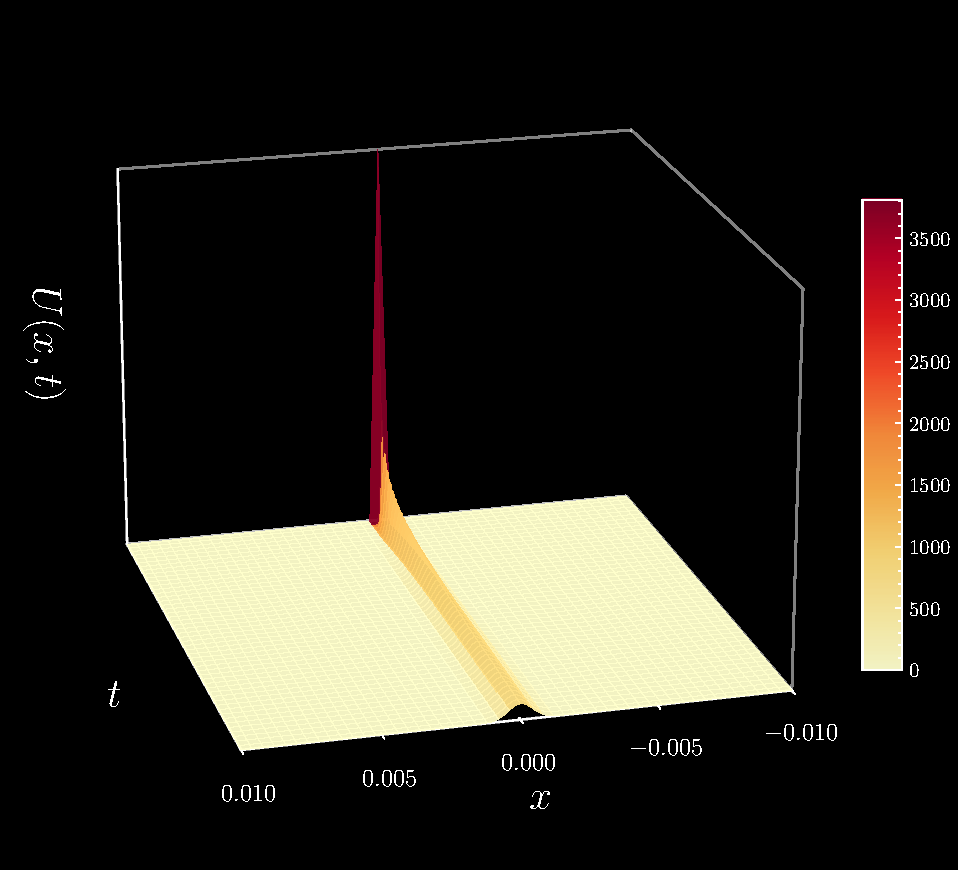
\includegraphics[width=1.0\textwidth]{../chap8/sec8.3/chap8sec8.3ex2.pdf}
\end{center}

% QUESTION 3
\qs{8.3.3}{To solve \( u_{t} = cu_{xx} \) for a bar between \( x = 0 \) and \( x = 1 \), the basis functions are still \( \sin\!\left(k \pi x \right) \) (with \( u = 0 \) at the ends). What are the eigenvalues \( \lambda_{k} \) that go into the solution \( \sum b_{k}\!\left( 0 \right)e^{-\lambda_{k}t}\sin\!\left(k \pi x \right) \)?}

With the diffusion constant, we now have
\[
	\lambda_{k} = ck^{2}\pi^{2}
\]
On the left, \( \partial u / \partial t \) gives us \( ck^{2}\pi^{2} \). On the right, \( \partial^{2}u / \partial x^{2} \) gives us \( k^{2}\pi^{2} \). Multiply by the diffusivity constant for equality.

\vspace{12pt}

\newpage
% QUESTION 4
\qs{8.3.4}{Following Problem 3, solve \( u_{t} = cu_{xx} \) when the initial temperature is \( u_{0} = 1 \) for \( \frac{1}{4} \le x \le \frac{3}{4} \) (and \( u_{0} = 0 \) on the first and last quarters of the bar). The problem is to find the coefficients \( b_{k}\!\left( 0 \right) \) for that initial temperature.}

First, derive the Fourier series for the even square wave
\[
	SW \!\left( x \right) = \begin{cases}
		1 & \text{for } -\frac{3}{4} < x < -\frac{1}{4} \\
		0 & \text{for } -1 < x < -\frac{3}{4} \text{ and } -\frac{1}{4} < x < \frac{1}{4} \text{ and } \frac{3}{4} < x < 1 \\
		1 & \text{for } \frac{1}{4} < x < \frac{3}{4}
	\end{cases}
\]
An intuitive approach here is to alter the Fourier series for the square wave given in the book's equation (6):
\[
	\frac{4}{\pi} \sum_{k = 1}^{\infty} \frac{\sin\!\left[\!\left( 2k - 1 \right) \pi x \right] }{2k - 1} 
\]
First is to offset the horizontal position by \( 3 / 4 \) and adjust the periodicity by a factor of 2: instead of the width of the period being \( 1 \), it is now \( 1 / 2 \).

\[
	SW \!\left( x \right) = \frac{4}{\pi} \sum_{k = 1}^{\infty} \frac{\sin\!\left[\!\left( 4k - 2 \right) \pi \!\left( x + \frac{3}{4} \right)\right] }{2k - 1}
\]
By the angle difference identity for sine and reducing trigonometric functions to even-odd sign parity, this becomes
\[
	SW \!\left( x \right) = \frac{4}{\pi} \sum_{k = 1}^{\infty} \frac{\!\left( -1 \right)^{k}}{2k - 1} \cos\!\left[ \!\left( 4k - 2 \right)\pi x \right]
\]
Lastly, we need to scale the amplitude and vertically offset the square wave. For this problem, multiply the sum by \( 1 / 2 \) (since the wave peaks between \( 0 \) and \( 1 \)) and add \( 1 / 2 \) (since it is symmetric about \( u = 1 / 2 \)). This gives us our transformed square wave.
\[
	SW \!\left( x \right) = \frac{1}{2} + \frac{2}{\pi} \sum_{k = 1}^{\infty} \frac{\!\left( -1 \right)^{k}}{2k - 1}\cos\!\left[ \!\left( 4k - 2 \right) \pi x \right] 
\]
The corresponding coefficients are then
\[
	b_{k}\!\left( 0 \right) = \frac{2}{\pi}\frac{\!\left( -1 \right)^{k}}{2k - 1}
\]

\begin{center}
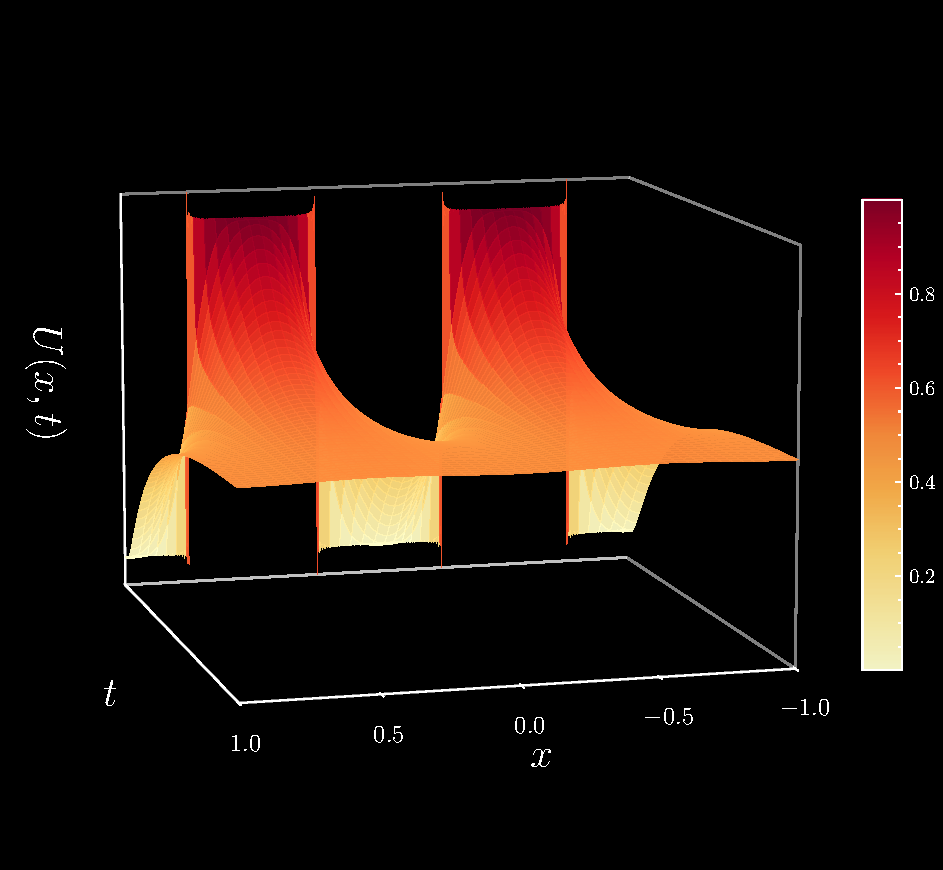
\includegraphics[width=1.0\textwidth]{../chap8/sec8.3/chap8sec8.3ex4.pdf}
\end{center}

% QUESTION 5
\qs{8.3.5}{Solve the heat equation \( u_{t} = u_{xx} \) from a point source \( u \!\left( x, 0 \right) = \delta \!\left( x \right) \) with free boundary conditions \( u'\!\left( \pi, t \right) = u'\!\left( -\pi, t \right) = 0 \). Use the infinite cosine series \( \delta \!\left( x \right) = \!\left( 1 + 2 \cos\!\left(x\right) + 2 \cos\!\left( 2x \right) + \cdots \right) / 2 \pi \) multiplied by time decay factors \( b_{k}\!\left( t \right) \).}

Incorporating the time decay factors, the solution is
\[
	u \!\left( x,t \right) = \frac{1}{2 \pi} + \frac{1}{\pi} \sum_{k=1}^{\infty} e^{-k^{2}\pi^{2}t}\cos\!\left(kx\right)  
\]
Note that the Fourier coefficients to the cosines series provide us with the \( b_{k}\!\left( 0 \right) \) constants. Differentiating with respect to \( x \), we get
\[
	u'\!\left( x,t \right) = -\frac{1}{\pi} \sum^{\infty}_{k=1} e^{-k^{2}\pi^{2}t} k \sin\!\left(kx\right)
\]
From which it is immediately apparent that
\[
	u'\!\left( \pi, t \right) = u'\!\left( -\pi, t \right) = 0 
\]

\begin{center}
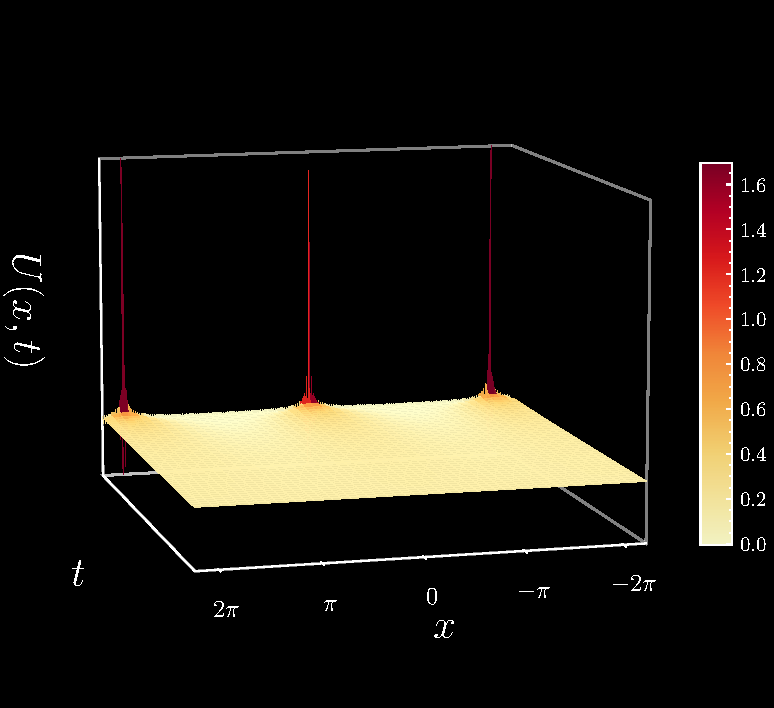
\includegraphics[width=1.0\textwidth]{../chap8/sec8.3/chap8sec8.3ex5.pdf}
\end{center}

\vspace{12pt}
% QUESTION 6
\qs{8.3.6}{(Bar from \( x = 0 \) to \( x = \infty \)) Solve \( u_{t} = u_{xx} \) on the positive half of an infinite bar, starting from the shifted delta function \( u_{0} = \delta \!\left( x - a \right) \) at a point \( x = a > 0 \). Here is a way to use the full-bar heat kernel \( U \) in (14), and still keep \( u = 0 \) at \( x = 0 \).

Imagine a negative point source at \( x = -a \). Solve the heat equation on the fully infinite bar, including both sources in \( u_{0} = \delta \!\left( x - a \right) - \delta \!\left( x + a \right) \) at \( t = 0 \). Your solution (a difference of heat kernels) will stay zero at the boundary \( x = 0 \) (\textit{Why}?). Then it must be the correct solution on the half-bar, since it started correctly.}

Using equation (14) and invoking superposition, our solution is
\[
	u \!\left( t,x \right) = \frac{1}{\sqrt{4 \pi t}} \!\left[ e^{-\!\left( x - a \right)^{2} / 4t} - e^{-\!\left( x + a \right)^{2} / 4t} \right] 
\]
Note that at \( x = 0 \), \( u \!\left( t,0 \right) = 0 \). This method of solution is called the \textbf{method of images}. It is called so because of the trick in dropping in another source that generates the desired boundary condition.

For \( a = 1 \), we can graph the solution as 
\begin{center}
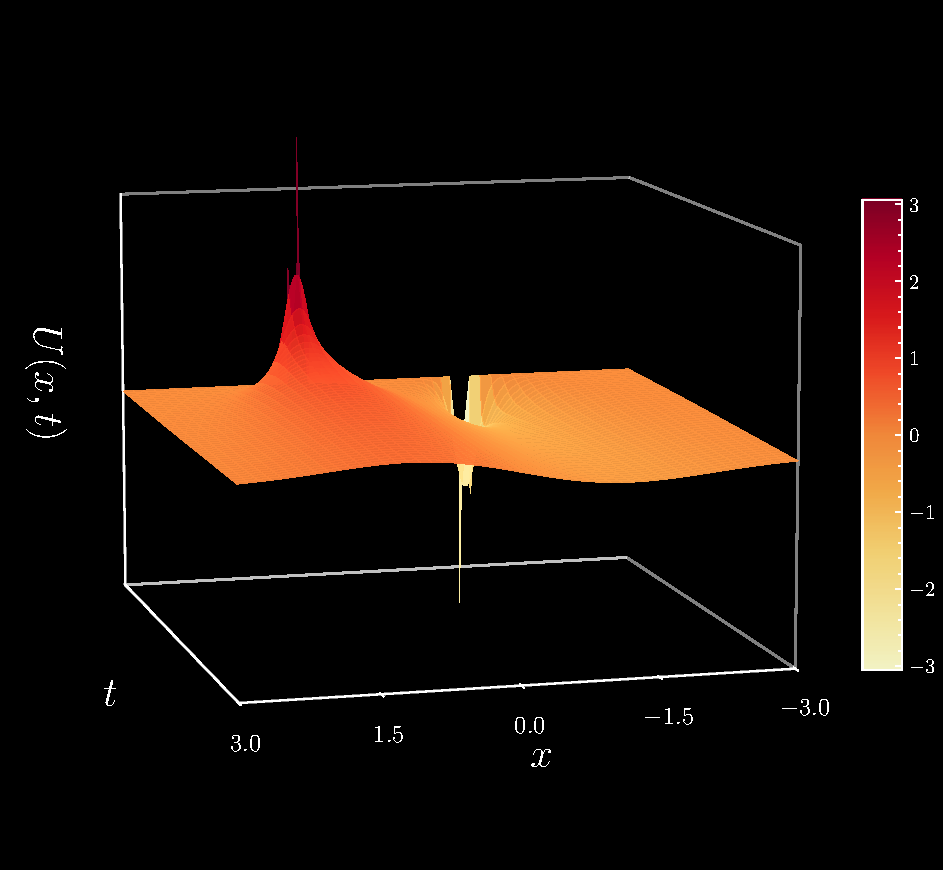
\includegraphics[width=1.0\textwidth]{../chap8/sec8.3/chap8sec8.3ex6.pdf}
\end{center}

\vspace{12pt}
% QUESTION 7
\qs{8.3.7}{Check that the basis functions \( s_{k} = \sin\!\left(k + \frac{1}{2}\right) \pi x \) are orthogonal over \( 0 \le x \le 1 \). Find a formula for the coefficient \( B_{4} \) in the Fourier series \( F \!\left( x \right) = \sum B_{k}s_{k} \). (Multiply by \( s_{4}\!\left( x \right) \) and integrate, to isolate \( B_{4} \).)}

Let \( k_{1} \neq k_{2} \) be integers. Then we can ascertain
\begin{align*}
	\int^{1}_{0} \sin\!\left( k_{1} + \frac{1}{2} \right) \pi x \sin\!\left( k_{2} + \frac{1}{2} \right) \pi x \, dx & = \frac{1}{2} \int^{1}_{0} \!\left[ \cos\!\left( k_{1} - k_{2} \right) \pi x - \cos\!\left( k_{1} + k_{2} + 1 \right) \pi x \right] \, dx \\
	 & = \frac{1}{2 \pi} \!\left[ \frac{\sin\!\left( k_{1} - k_{2} \right) \pi}{k_{1} - k_{2}} - \frac{\sin\!\left( k_{1} + k_{2} + 1 \right) \pi}{k_{1} + k_{2} + 1} \right] \\
	 & = 0
\end{align*}
This is true for any choice of \( k_{1} \), \( k_{2} \). Invoking orthogonality, we can then calculate
\begin{align*}
	\int^{1}_{0} F \!\left( x \right) s_{4}\!\left( x \right) \, dx & = \int^{1}_{0} \sum B_{k}s_{k}s_{4} \, dx \\
	 & = B_{4} \int^{1}_{0} \sin^{2}\!\left( \frac{9 \pi x}{2} \right) \, dx \\ 
	 & = \frac{B_{4}}{2} \\
\end{align*}
Leaving us with
\[
	B_{4} = 2 \int^{1}_{0} F \!\left( x \right)s_{4}\!\left( x \right) \, dx  
\]

% QUESTION 8
\qs{8.3.8}{The basis functions \( \sin\!\left(k + \frac{1}{2}\right) \pi x \) are for \textbf{fixed-free} boundaries (\( u = 0 \) at \( x = 0 \) and \( u' = 0 \) at \( x = 1 \)). What are the basis functions for \textbf{free-fixed boundaries} (\( u' = 0 \) at \( x = 0 \) and \( u = 0 \) at \( x = 1 \))?}

For free-fixed boundaries, our basis functions are \( \cos\!\left(k + \frac{1}{2}\right) \pi x \). Easy to verify that the free-fixed boundary conditions are met.

\vspace{12pt}
% QUESTION 9
\qs{8.3.9}{Suppose \( \pmb{u_{t} = u_{xx} - u} \) with boundary condition \( u = 0 \) at \( x = 0 \) and \( x = 1 \). Find the new numbers \( \lambda_{k} \) in the general solution \( u = \sum b_{k}\!\left( 0 \right) e^{-\lambda_{k}t} \sin\!\left(k \pi x\right) \). (Previously \( \lambda_{k} = -k^{2}\pi^{2} \), now there is a new term in \( \lambda \) because of \( -u \).)}

The additional \( -u \) term adds one to the eigenvalue after canceling the negative, giving us \( \lambda_{k} = k^{2}\pi^{2} + 1 \).

\vspace{12pt}
% QUESTION 10
\qs{8.3.10}{Explain each step in equation (13). Solve \( dU / dx = -xU / 2t \) to reach \( U = e^{-x^{2} / 4t} \). How do the known infinite integrals \( \int e^{-x^{2}} \, dx = \sqrt{\pi} \) and \( \int u \, dx = 1 \) lead to the factor \( 1 / \sqrt{4 \pi t} \)?}

The integration by parts proceeds as follows: let \( a = ie^{ikx} \) and \( db = e^{-k^{2}t}k \, dk \). Then \( da = -xe^{ikx} \, dk \) and \( b = -e^{-k^{2}t} / 2t \). Combining the parts (don't forget the \( 1 / 2 \pi \) term) gives
\begin{align*}
	\frac{d U}{d x} & = -ie^{-k^{2}t}e^{ikx} \Big|^{\infty}_{-\infty} - \frac{1}{4 \pi t}\int^{\infty}_{-\infty} \!\left( e^{-k^{2}t} \right)\!\left( xe^{ikx} \right) \, dk \\
			& = -\frac{1}{4 \pi t}\int^{\infty}_{-\infty} \!\left( e^{-k^{2}t} \right)\!\left( xe^{ikx} \right) \, dk \\
			& = -\frac{xU}{2t}
\end{align*}
Separating variables, we can deduce from \( dU / dx = -xU / 2t \) that
\[
	\int \frac{dU}{U} = -\int \frac{x}{2t} \, dx \quad \implies \quad \ln\!\left(U\right) = -\frac{x^{2}}{2t} + C \quad \implies \quad U = ce^{-x^{2} / 2t}
\]
The normalization constant \( c \) follows from the requirement that
\[
	\int^{\infty}_{-\infty} ce^{-x^{2} / 2t} \, dx = 1 
\]
which is true only when \( c = 1 / \sqrt{4 \pi t} \).

\vspace{12pt}
% QUESTION 11
\qs{8.3.11}{(\textbf{Shift invariance}) What is the solution to \( u_{t} = u_{xx} \) starting from \( \pmb{\delta \!\left( x - a \right)} \) at \( t = 0 \)?}

Equation (18): an integral of shifted heat kernels.
\[
	u \!\left( t,x \right) = \frac{1}{\sqrt{4 \pi t}} \int^{\infty}_{-\infty} u_{0}\!\left( a \right)e^{-\!\left( x - a \right)^{2} / 4t} \, da  
\]

% QUESTION 12
\qs{8.3.12}{What are basis functions \( A \!\left( x,y \right) \) for heat flow in a square plate, when \( u = 0 \) along the four sides \( x = 0 \), \( x = 1 \), \( y = 0 \), \( y = 1 \)? The heat equation is \( u_{t} = u_{xx} + u_{yy} \). Find eigenfunctions for \( A_{xx} + A_{yy} = \lambda A \) that satisfy the boundary conditions.

The first eigenfunction is \( A_{11} = \sin\!\left(\pi x\right) \sin\!\left(\pi y\right) \). Find the eigenvalues \( \lambda \).}

For heat flowing out of the perimeter of the square, we have basis functions
\[
	A \!\left( x,y \right) = \sin\!\left(m \pi x\right) \sin\!\left(n \pi y\right) 
\]
The eigenfunctions and corresponding eigenvalues are
\[
	- \pi^{2} \!\left( m^{2} + n^{2} \right) \sin\!\left(m \pi x\right) \sin\!\left(n \pi y\right) = \lambda_{m,n} \sin\!\left(m \pi x\right) \sin\!\left(n \pi y\right) 
\]
\[
	\implies \quad \lambda_{m,n} = -\pi^{2} \!\left( m^{2} + n^{2} \right)
\]

% QUESTION 13
\qs{8.3.13}{Substitute \( U = e^{-x^{2} / 4t} / \sqrt{4 \pi t} \) to show that this heat kernel solves \( U_{t} = U_{xx} \).}

Calculate
\[
	U_{t} = \!\left[ \frac{x^{2}}{4t^{2}} - \frac{1}{2t} \right] \frac{e^{-x^{2} / 4t}}{\sqrt{4 \pi t}} = U_{xx} 
\]

\newpage
\subsection{\textsf{8.4 - The Wave Equation}}

\textbf{Problems 1-4 are about the one-way wave equation \( \pmb{\partial u / \partial t = c \partial u / \partial x} \).}

% QUESTION 1
\qs{8.4.1}{Suppose \( u \!\left( 0,x \right) = \sin\!\left(2x\right) \). What is the solution to \( u_{t} = cu_{x} \)? At which times \( t_{1} \), \( t_{2} \), ... will the solution return to the initial condition \( \sin\!\left(2x\right) \)?}

The solution is \( u \!\left( t,x \right) = \sin\!\left(2 \!\left( x + ct\right) \right) \). The initial condition is returned to for all times \( t_{k} = k \pi / c \).

\vspace{12pt}

% QUESTION 2
\qs{8.4.2}{Suppose \( u_{0}\!\left( x \right) = \delta \!\left( x \right) \), a big bang at the origin of the one-dimensional universe. At time \( t \) the bang is heard at the point \( x = \) \underline{\qquad}. For \( u_{tt} = c^{2}u_{xx} \) the bang will reach the two points \( x = \) \underline{\qquad} and \( x = \) \underline{\qquad} at time \( t \).}

In the one-directional case, the solution is \( u \!\left( t,x \right) = \delta \!\left( x + ct \right) \) and the bang will be heard at \( x = -ct \). For two directions, we have
\[
	u \!\left( t,x \right) = \frac{1}{2} \!\left[ \delta \!\left( x - ct \right) + \delta \!\left( x + ct \right) \right]
\]
in which the bang is heard at \( x = ct \) and \( x = -ct \) at time \( t \).

\vspace{12pt}
% QUESTION 3
\qs{8.4.3}{\begin{enumerate}[label=(\alph*)]
	\item Integrate both sides of \( u_{t} = cu_{x} \) from \( x = -\infty \) to \( \infty \) to prove that the total mass \( M = \int u \, dx \) is constant: \( dM / dt = 0 \).
	\item Multiply by \( u \) and integrate both sides of \( uu_{t} = cuu_{x} \) to prove that \( E = \int u^{2} \, dx \) is constant.
\end{enumerate}}

\begin{enumerate}[label=(\alph*)]
	\item The problem should specify that \( u \rightarrow 0 \) as \( \abs{x} \rightarrow 0 \). Intuitively, we should also conceive of \( u \) as a ``density'' of sorts. Combined, these insights suggest a spatial localization of the source of the wave (for instance, if I perturb the water of the Atlantic Ocean off of the coast of Coney Island, New York, it is completely unlikely that someone at Normandy beach in France will know about it). Derive
		\begin{align*}
			\int^{\infty}_{-\infty} u_{t} \, dx & = \frac{d }{d t} \int^{\infty}_{-\infty} u \, dx \\
			\int^{\infty}_{-\infty} cu_{x} \, dx & = \int^{\infty}_{-\infty} cu_{0}'\!\left( x + ct \right) \, dx \\
							     & = c \!\left[ u_{0}\!\left( \infty + ct \right) - u_{0}\!\left( -\infty + ct \right) \right] \\
							     & = 0
		\end{align*}
		Equating the two sides establishes conservation of mass.
	\item Now we derive conservation of energy.
		\begin{align*}
			\int^{\infty}_{-\infty} uu_{t} \, dx & = \frac{1}{2} \frac{d }{d t} \int^{\infty}_{-\infty} u^{2} \, dx \\
			\int^{\infty}_{-\infty} cuu_{x} \, dx & = \frac{c}{2} \int^{\infty}_{-\infty} \frac{d }{d x} u^{2} \, dx \\
							      & = 0
		\end{align*}
\end{enumerate}

% QUESTION 4
\qs{8.4.4}{Is the wave \( u \!\left( t,x \right) = u_{0}\!\left( x + ct \right) \) traveling left or right if \( c > 0 \)? To solve \( u_{t} = cu_{x} \) on the halfline \( 0 \le x \le \infty \), why is a boundary condition \( u \!\left( t,0 \right) = 0 \) \textit{not wanted}? With \( c < 0 \) and waves in the opposite direction, that condition is appropriate.}

For positive \( c \), the wave is traveling left. The given boundary condition is problematic as it forces \( u = 0 \) for all \( t \) at \( x = 0 \). In other words, whichever initial conditions the solution as, its profile at the outflow must be zero. With negative \( c \), the wave travels right from the inflow point at \( x = 0 \), and the boundary condition simply requires that \( u \) begins at zero.

\vspace{12pt}
\textbf{Problems 5-9 are about the one-dimensional wave equation 
\[
	\pmb{\partial^{2}u / \partial t^{2} = c^{2}\partial^{2}u / \partial x^{2}}
\]}

% QUESTION 5
\qs{8.4.5}{A ``box of water'' has \( u_{0}\!\left( x \right) = 1 \) for \( -1 \le x \le 1 \). Starting with zero velocity \( v_{0}\!\left( x \right) \), the wave equation \( u_{tt} = c^{2}u_{xx} \) is solved by \( u \!\left( t,x \right) = \frac{1}{2}u_{0}\!\left( x + ct \right) + \frac{1}{2}u_{0}\!\left( x - ct \right) \). Graph this solution for small \( t = \frac{1}{2}c \) and large \( t = 3c \).}

For simplicity, set \( c = 1 \). The intuition is clear: the box of water ``separates'' into two waves, propagating anti-parallel from the center.

\begin{center}
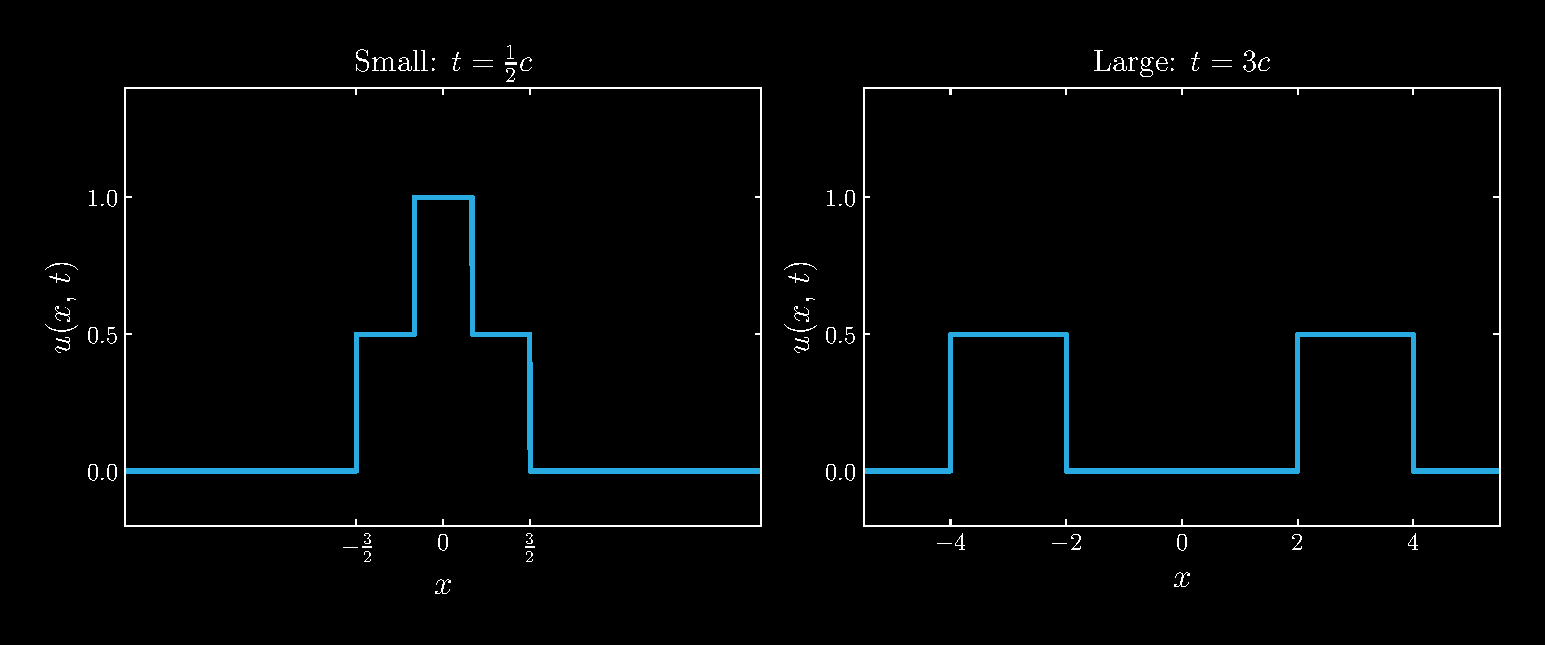
\includegraphics[width=1.0\textwidth]{../chap8/sec8.4/chap8sec8.4ex5.pdf}
\end{center}

% QUESTION 6
\qs{8.4.6}{Under a flat ocean with \( u_{0}\!\left( x \right) = 1 \), an earthquake produces \( v_{0}\!\left( x \right) = \delta \!\left( x \right) \). A one-dimensional tsunami starts moving with speed \( c \). What is the solution (7) at time \( t \)?}

In equation (7), the last term becomes
\[
	\frac{1}{2c} \int^{x + ct}_{x - ct} \delta \!\left( x \right) \, dx = \begin{cases}
		0, & 0 \not\in \!\left[ x - ct, x + ct \right] \\
		1, & 0 \in \!\left[ x - ct, x + ct \right]
	\end{cases}  
\]
And since the ocean is flat, the first two terms simply sum to unity.
This all corresponds to solution
\[
	u \!\left( t,x \right) = 1 + \begin{cases}
		\frac{1}{2c}, & \abs{x} \le ct \\
		0 & \text{otherwise} \\
	\end{cases}
\]

% QUESTION 7
\qs{8.4.7}{Separation of variables gives \( u \!\left( t,x \right) = \sin\!\left(nx\right) \sin\!\left(nct\right) \) and three other similar solutions to \( u_{tt} = c^{2}u_{xx} \). \textit{What are those three}? Which complex functions \( e^{ikx}e^{i \omega t} \) solve the wave equation?}

We also have
\begin{align*}
	u \!\left( t,x \right) & = \cos\!\left(nx\right) \cos\!\left(nct\right) \\
	u \!\left( t,x \right) & = \sin\!\left(nx\right) \cos\!\left(nct\right) \\ 
	u \!\left( t,x \right) & = \cos\!\left(nx\right) \sin\!\left(nct\right) 
\end{align*}
From superposition, we may deduce that complex functions of the form
\[
	u \!\left( t,x \right) = e^{inx}e^{inct} 
\]
comprehensively encapsulate the four trigonometric solutions to the wave equation.

\vspace{12pt}

% QUESTION 8
\qs{8.4.8}{The 3D wave equation \( u_{tt} = u_{xx} + u_{yy} + u_{zz} \) becomes 1D when \( u \) has spherical symmetry: \( u \) depends only on \( r \) and \( t \).
\[
	r = \sqrt{x^{2} + y^{2} + z^{2}} \quad \text{and} \quad \frac{\partial^{2}u}{\partial t^{2}} = \frac{\partial^{2}u}{\partial r^{2}} + \frac{2}{r}\frac{\partial u}{\partial r} 
\]
\begin{enumerate}[label=(\alph*)]
	\item \textit{Multiply by} \( r \) \textit{to find} \( \!\left( ru \right)_{tt} = \!\left( ru \right)_{rr} \)! Then \( ru \) is a function of \( r + t \) and \( r - t \).
	\item Describe the solution \( ru = \delta \!\left( r - t - 1 \right) \). This spherical sound wave has the radius \( r = \) \underline{\qquad} at \( t = 8 \).
\end{enumerate}}

\begin{enumerate}[label=(\alph*)]
	\item Derive
	\begin{align*}
		\!\left( ru \right)_{tt} & = r_{tt}u + ru_{tt} \\
					 & = ru_{tt} \\
		\!\left( ru \right)_{r} & = u + ru_{r} \\ 
		\!\left( ru \right)_{rr} & = u_{r} + \!\left( u_{r} + ru_{rr} \right) \\
					& = 2u_{r} + ru_{rr}
	\end{align*}
	\item We can analogize this to the front of an ``explosion'' with initial radius 1. As time progresses to \( t = 8 \), the explosion front grows to \( r = 9 \).
\end{enumerate}

\vspace{12pt}

% QUESTION 9
\qs{8.4.9}{The wave equation along a bar with density \( \rho \) and stiffness \( k \) is \( \pmb{\!\left( \rho u_{t} \right)_{t} = \!\left( ku_{x} \right)_{x}} \). What is the velocity \( c \) in \( u_{tt} = c^{2}u_{xx} \)? What is \( \omega \) in \( u = \sin\!\left(\pi x / L\right) \cos\!\left(\omega t\right) \)?}

Assuming constancy in the density and stiffness, we have \( c = \sqrt{k / \rho} \). It follows that
\[
	\omega = \frac{\pi}{L}\sqrt{\frac{k}{\rho}} 
\]

% QUESTION 10
\qs{8.4.10}{The small vibrations of a beam satisfy the fourth order equation \( u_{tt} = -c^{2}u_{xxxx} \). Look for solutions \( u = X \!\left( x \right) T \!\left( t \right) \) and find separate equations for the functions \( X \) and \( T \). Then find four solutions \( X \!\left( x \right) \) when \( T \!\left( t \right) = \cos\!\left(\omega t\right) \).}

For our setup, we have in this equation
\[
	X \!\left( x \right)T''\!\left( t \right) = -c^{2}X''''\!\left( x \right)T \!\left( t \right) 
\]
Divide through by \( c^{2}X \!\left( x \right)T \!\left( t \right) \) and set equal to \( -\omega^{2} \) to get
\[
	\frac{T''\!\left( t \right)}{c^{2}T \!\left( t \right)} = -\frac{X''''\!\left( x \right)}{X \!\left( x \right)} = -\omega^{2}
\]
Then to solve the temporal and spatial component respectively, we satisfy
\[
	T''\!\left( t \right) = -c^{2}\omega^{2}T \!\left( t \right) \qquad X''''\!\left( x \right) = \omega^{2}X \!\left( x \right)
\]
Then \( T \!\left( t \right) = \sin\!\left(c \omega t\right) \) or \( \cos\!\left(c \omega t\right) \), and \( X \!\left( x \right) = \sin\!\left(\sqrt{\omega}x\right) \), \( \cos\!\left(\sqrt{\omega}x\right) \), \( e^{\sqrt{\omega}x} \), or \( e^{-\sqrt{\omega}x} \).

When \( T \!\left( t \right) = \cos\!\left(\omega t\right) \), solutions for \( X \!\left( x \right) \) include \( \sin\!\left(ax\right) \), \( \cos\!\left(ax\right) \), \( e^{ax} \), and \( e^{-ax} \), where \( a = \sqrt{\omega / c} \).

The key difference here is whether you divide through by \( c^{2} \) in deriving the temporal and spatial equations, which will determine whether \( c \) shows up in one or the other.

\vspace{12pt}

% QUESTION 11
\qs{8.4.11}{If that beam is clamped (\( u = 0 \) and \( \partial u / \partial x = 0\) at both ends \( x = 0 \) and \( x = L \)), show that the frequencies \( \omega \) in Problem 10 must have \( \cos\!\left(\omega L\right) \cosh\!\left(\omega L\right) = 1 \).}

In setting up the solution, we will rewrite the basis functions \( e^{ax} \) and \( e^{-ax} \) in terms of \( \cosh\!\left(ax\right) \) and \( \sinh\!\left(ax\right) \). The general set of solutions of the spatial component and its derivative will be of form
\begin{align*}
	X \!\left( x \right) & = a_{1}\sin\!\left(\omega x\right) + a_{2}\cos\!\left(\omega x\right) + a_{3}\sinh\!\left(\omega x\right) + a_{4}\cosh\!\left(\omega x\right) \\
	X'\!\left( x \right) & = \omega \!\left[ a_{1}\cos\!\left(\omega x\right) - a_{2}\sin\!\left(\omega x\right) + a_{3}\cosh\!\left(\omega x\right) + a_{4}\sinh\!\left(\omega x\right) \right]
\end{align*}
We do not wish to impose any constraints on the coefficients beyond those that stem from the boundary conditions; remember this fact for later.

Now, impose the boundary conditions at \( x = 0 \).
\begin{align*}
	X \!\left( 0 \right) & = a_{2} + a_{4} = 0 \\
	X'\!\left( 0 \right) & = \omega \!\left( a_{1} + a_{3} \right) = 0
\end{align*}
Immediately, we reduce four unknowns to two: \( a_{4} = -a_{2} \) and \( a_{3} = -a_{1} \). Taking this into account while incorporating the boundary conditions at \( x = L \), we derive the system of equations
\begin{align*}
	X \!\left( L \right) & = a_{1}\!\left[ \underbrace{\sin\!\left(\omega L\right) - \sinh\!\left(\omega L\right)}_{p} \right] + a_{2}\!\left[ \underbrace{\cos\!\left(\omega L\right) - \cosh\!\left(\omega L\right)}_{q} \right] = 0 \\
	X'\!\left( L \right) & = a_{1}\!\left[ \underbrace{\cos\!\left(\omega L\right) - \cosh\!\left(\omega L\right)}_{q} \right] - a_{2}\!\left[ \underbrace{\sin\!\left(\omega L\right) + \sinh\!\left(\omega L\right)}_{r} \right] = 0
\end{align*}
where we divide the second equation through by \( \omega \) as we won't need that. Rewriting this as a matrix equation, we have
\[
	\begin{bmatrix}
		p & q \\
		q & -r \\
	\end{bmatrix}
	\begin{bmatrix}
		a_{1} \\
		a_{2} \\
	\end{bmatrix} = 
	\begin{bmatrix}
		0 \\
		0 \\
	\end{bmatrix}
\]
Now, recall that we have to account for a \textit{general} set of solutions. This means that there cannot be a unique solution for this system of equations. Specifically, we must have infinitely many solutions (coefficients). Therefore, we can immediately conclude that we must have \textit{zero determinant}. Calculating, we can come to our final deduction:
\begin{align*}
	\det & = -pr - q^{2} \\
	 & = -\!\left[ \sin\!\left(\omega L\right) - \sinh\!\left(\omega L\right) \right]\!\left[ \sin\!\left(\omega L\right) + \sinh\!\left(\omega L\right) \right] - \!\left[ \cos\!\left(\omega L\right) - \cosh\!\left(\omega L\right) \right]^{2} \\ 
	 & = -\!\left[ \sin^{2}\!\left(\omega L\right) + \cos^{2}\!\left(\omega L\right) \right] - \!\left[ \cosh^{2}\!\left(\omega L\right) - \sinh^{2}\!\left(\omega L\right) \right] + 2 \cos\!\left(\omega L\right) \cosh\!\left(\omega L\right) \\
	 & = -2 + 2 \cos\!\left(\omega L\right) \cosh\!\left(\omega L\right) \\
	 & = 0
\end{align*}
which forces \( \cos\!\left(\omega L\right) \cosh\!\left(\omega L\right) = 1 \).

\vspace{12pt}

\textbf{Problems 12-16 solve the wave equation with boundary conditions at \( \pmb{x = 0} \) and \( \pmb{x = L} \).}

\vspace{12pt}

% QUESTION 12
\qs{8.4.12}{A string plucked halfway along has \( u_{0}\!\left( x \right) = \delta \!\left( x - \frac{L}{2} \right) \) and \( v_{0}\!\left( x \right) = 0 \). Find the Fourier coefficients \( b_{k} \) from equation (18). Write the first three terms of the Fourier series solution in (16).}

The Fourier coefficients are
\[
	b_{k} = \frac{\displaystyle{\int^{L}_{0} \delta \!\left( x - \frac{L}{2} \right)\sin\!\left(\frac{k \pi x}{L}\right) \, dx}}{\displaystyle{\int^{L}_{0} \sin^{2}\!\left(\frac{k \pi x}{L}\right) \, dx}} = \frac{\displaystyle{4k \pi \sin\!\left(\frac{k \pi}{2}\right)}}{2kL \pi - L \sin\!\left(2k \pi\right)} = \frac{2}{L}\sin\!\left(\frac{k \pi}{2}\right) 
\]
We see that \( b_{k} \) vanishes for even \( k \). Therefore, the full Fourier series is
\[
	u \!\left( t,x \right) = \sum^{\infty}_{k = 1} \frac{2}{L}\!\left( -1 \right)^{k + 1} \sin\!\left(\frac{\!\left( 2k - 1 \right)\pi x}{L}\right) \cos\!\left(\frac{\!\left( 2k - 1 \right)\pi ct}{L}\right) 
\]
And its first three terms are
\[
	u \!\left( t,x \right) \approx \frac{2}{L} \!\left[ \sin\!\left(\frac{\pi x}{L}\right) \cos\!\left(\frac{\pi ct}{L}\right) - \sin\!\left(\frac{3 \pi x}{L}\right) \cos\!\left(\frac{3 \pi ct}{L}\right) + \sin\!\left(\frac{5 \pi x}{L}\right) \cos\!\left(\frac{5 \pi ct}{L}\right) \right]
\]

\begin{center}
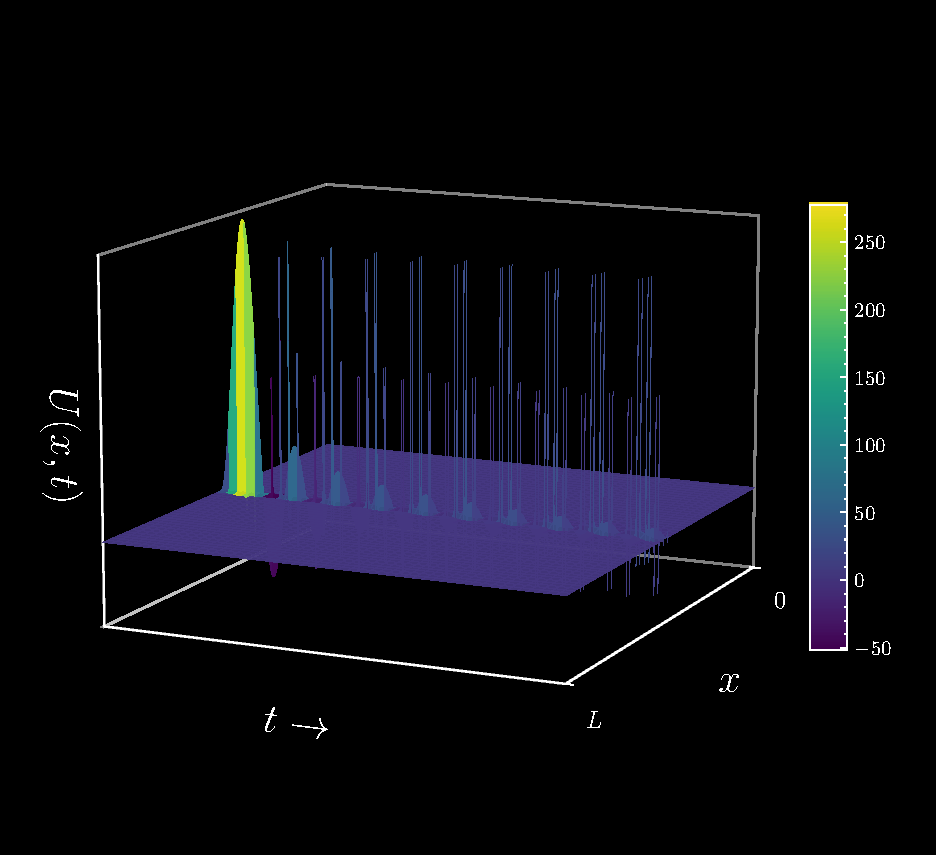
\includegraphics[width=1.0\textwidth]{../chap8/sec8.4/chap8sec8.4ex12.pdf}
\end{center}

% QUESTION 13
\qs{8.4.13}{Suppose the string starts with zero velocity \( v_{0}\!\left( x \right) \) from a \textit{hat function}: \( u_{0}\!\left( x \right) = 2x/L \) for \( x < L/2 \) and \( u_{0}\!\left( x \right) = 2 \!\left( L - x \right)/L \) for \( x > L/2 \). Find the Fourier coefficients \( b_{k} \) from (18) and the first two nonzero terms of \( u \!\left( t,x \right) \) in (16).}

Calculate
\[
	\frac{2}{L} \!\left[ \int^{L/2}_{0} x \sin\!\left(\frac{k \pi x}{L}\right) \, dx + \int^{L}_{L/2} \!\left( L - x \right)\sin\!\left(\frac{k \pi x}{L}\right) \, dx \right] = \frac{4L}{k^{2}\pi^{2}}\sin\!\left(\frac{k \pi}{2}\right)
\]
Divide through by \( \int^{L}_{0} \sin^{2}\!\left(k \pi x / L\right) \, dx = L / 2 \) to get as our Fourier coefficients
\[
	b_{k} = \frac{8}{k^{2}\pi^{2}}\sin\!\left(\frac{k \pi}{2}\right)  
\]
The coefficients vanish for even \( k \). Let \( k = 2n - 1 \). Then the solution is
\[
	u \!\left( t,x \right) = \sum^{\infty}_{n = 1} \frac{8}{\!\left( 2n - 1 \right)^{2}\pi^{2}} \!\left( -1 \right)^{n - 1}\sin\!\left(\frac{\!\left( 2n - 1 \right)\pi x}{L}\right) \cos\!\left(\frac{\!\left( 2n - 1 \right)\pi ct}{L}\right) 
\]

\begin{center}
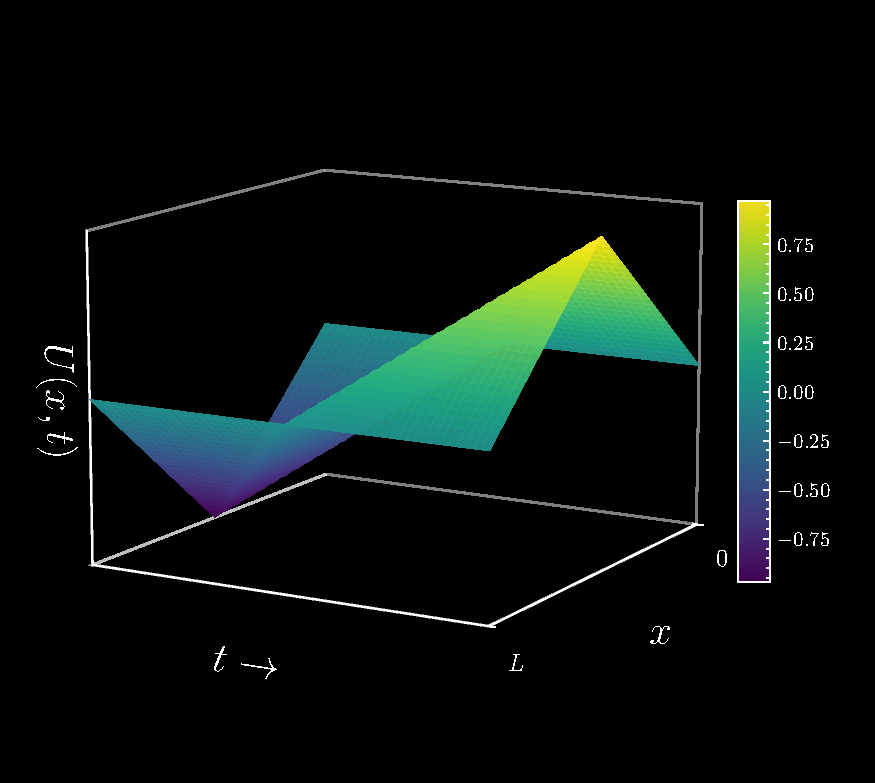
\includegraphics[width=1.0\textwidth]{../chap8/sec8.4/chap8sec8.4ex13.pdf}
\end{center}

% QUESTION 14
\qs{8.4.14}{Suppose the string starts with zero velocity \( v_{0}\!\left( x \right) \) from a \textit{box function}: \( u_{0}\!\left( x \right) = 1 \) for \( x < L/2 \). Find all the \( b_{k} \) in the solution \( u = \sum b_{k}\sin\!\left(k \pi x / L\right)\cos\!\left(k \pi ct / L\right) \).}

Calculate the Fourier coefficients
\[
	b_{k} = \frac{\displaystyle{\int^{L/2}_{0} \sin\!\left(\frac{k \pi x}{L}\right) \, dx }}{\displaystyle{\int^{L}_{0} \sin^{2}\!\left(\frac{k \pi x}{L}\right) \, dx}} = \frac{2}{k \pi} \!\left[ 1 - \cos\!\left(\frac{k \pi}{2}\right) \right]
\]

\begin{center}
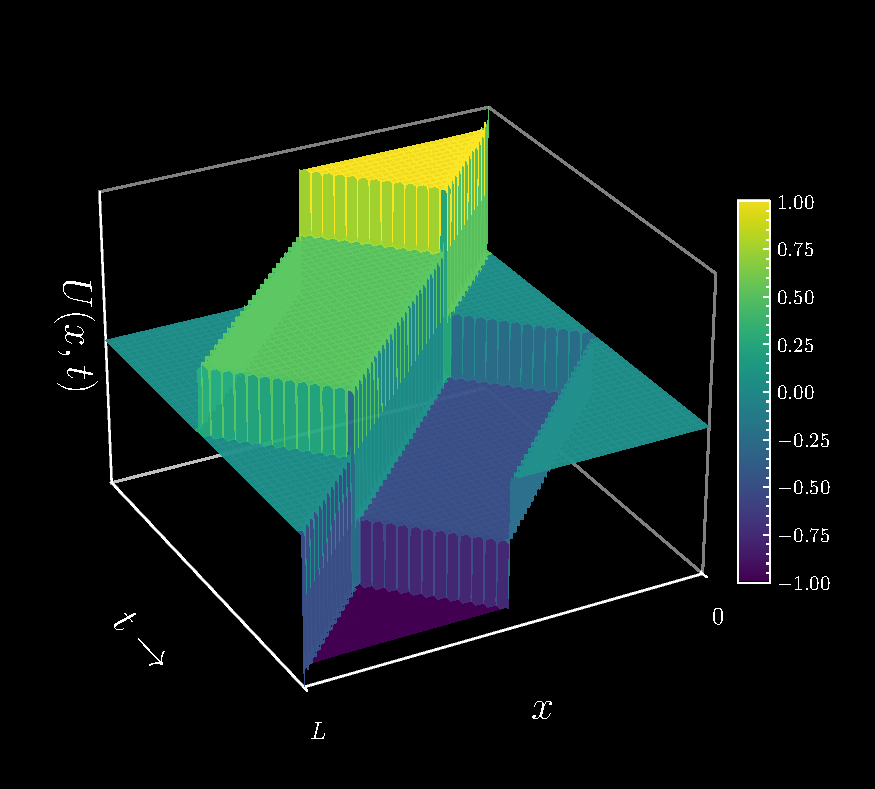
\includegraphics[width=1.0\textwidth]{../chap8/sec8.4/chap8sec8.4ex14.pdf}
\end{center}

% QUESTION 15
\qs{8.4.15}{The boundary condition at a \textit{free end} \( x = L \) is \( \partial u / \partial x = 0 \) instead of \( u = 0 \). Solve \( X'' + \omega^{2}X = 0 \) to find \( X \!\left( x \right) \) and all allowable \( \omega \)'s with this new condition. Then solve \( T'' + \omega^{2}c^{2}T = 0 \) to complete the solution \( u = \sum a_{n}X \!\left( x \right) T \!\left( t \right) \).}

Two null solutions: \( \sin\!\left(\omega x\right) \) and \( \cos\!\left(\omega x\right) \). Imposing the boundary conditions: \( u = 0 \) at \( x = 0 \) and \( \partial u / \partial x = 0 \) at \( x = L \), we must have \( X \!\left( x \right) = \sin\!\left(\omega x\right) \) where \( \omega L = \pi / 2 + n \pi \). We can then deduce the values of \( \omega_{n} \) are
\[
	\omega_{n} = \frac{\pi \!\left( 2n + 1 \right)}{2L} 
\]
For \( T \!\left( t \right) \), once again we have two null solutions: \( \sin\!\left(\omega c t\right) \) and \( \cos\!\left(\omega c t\right) \). Assuming initial condition of \( T' = v_{0} = 0 \), only the cosine term will survive. Our full solution is then
\[
	u = \sum^{\infty}_{n=0} a_{n}\sin\!\left(\omega_{n}x\right)\cos\!\left(\omega_{n}ct\right)  
\]
with \( \omega_{n} \) defined as above. Note the summation beginning at \( n = 0 \) in this case, so we start from \( \omega_{0} = \pi / 2L \).

\vspace{12pt}

% QUESTION 16
\qs{8.4.16}{What is the solution \( u \!\left( t,x \right) \) on a string of length \( L = 2 \) if \( u \!\left( 0,x \right) = \delta \!\left( x - 1 \right) \)? The end \( x = 0 \) is fixed by \( u \!\left( t,0 \right) = 0 \) and the end \( x = 2 \) is free: \( \partial u / \partial x \!\left( t,0 \right) = 0 \).}

Using the solution form of Problem 15, we calculate the Fourier coefficients as (note the denominator here is simply 1 with \( L = 2 \))
\[
	b_{n} = \int^{2}_{0} \delta \!\left( x - 1 \right)\sin\!\left(\omega_{n}x\right) \, dx = \sin\!\left(\omega_{n}\right) = \sin\!\left(\frac{\pi \!\left( 2n + 1 \right)}{4}\right)   
\]
With the boundary conditions, the solution is
\[
	u \!\left( t,x \right) = \sum^{\infty}_{n=0} \sin\!\left(\frac{\pi \!\left( 2n + 1 \right)}{4}\right) \sin\!\left(\frac{\pi \!\left( 2n + 1 \right)x}{4}\right) \cos\!\left(\frac{\pi \!\left( 2n + 1 \right)t}{4}\right) 
\]

\begin{center}
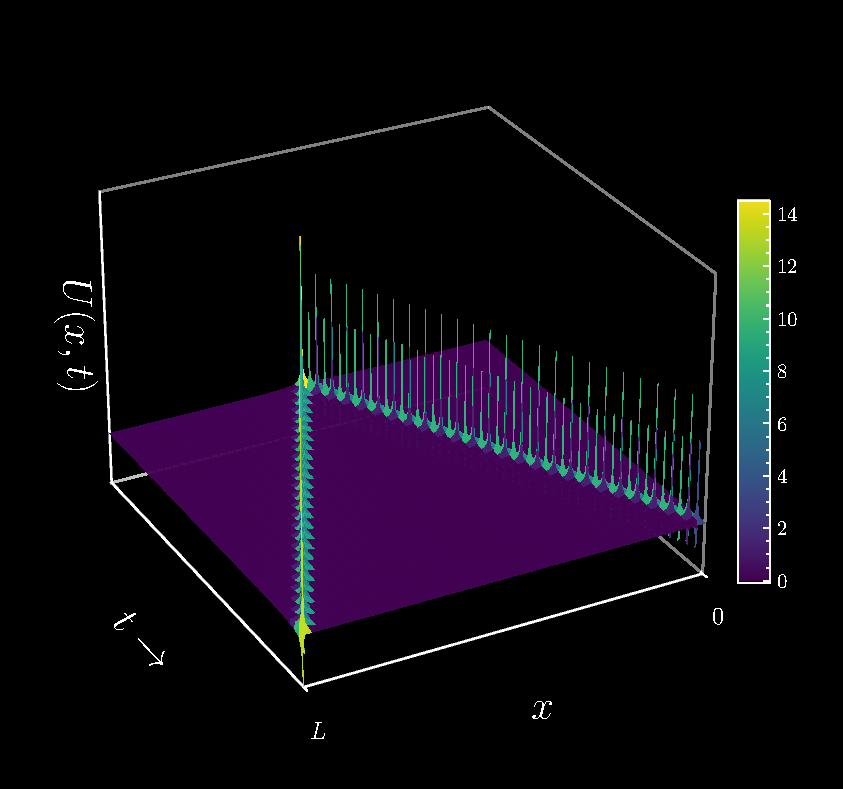
\includegraphics[width=1.0\textwidth]{../chap8/sec8.4/chap8sec8.4ex16.pdf}
\end{center}

\newpage

\subsection{\textsf{8.5 - The Laplace Transform}}
% QUESTION 1
\qs{8.5.1}{When the driving function is \( f \!\left( t \right) = \delta \!\left( t \right) \), the solution starting from rest is the \textbf{impulse response}. The impulse is \( \delta \!\left( t \right) \), the response is \( y \!\left( t \right) \). Transform this equation to find the \textbf{transfer function} \( Y \!\left( s \right) \). Invert to find the impulse response \( y \!\left( t \right) \).
\[
	y'' + y = \delta \!\left( t \right) \text{ with } y \!\left( 0 \right) = 0 \text{ and } y'\!\left( 0 \right) = 0 
\]}

Since \( \mathcal{L}\!\left[ y' \right] = s Y \!\left( s \right) - y \!\left( 0 \right) \), it follows that 
\[
	\mathcal{L}\!\left[ y'' \right] = s \mathcal{L}\!\left[ y' \right] - y'\!\left( 0 \right) = s^{2} \mathcal{L}\!\left[ y \right] - sy \!\left( 0 \right) - y'\!\left( 0 \right) 
\]
The Laplace transform of the delta function can be derived as 
\[
	\mathcal{L}\!\left[ \delta \!\left( t \right) \right] = \int^{\infty}_{0} \delta \!\left( t \right) e^{-st} \, dt = 1  
\]
Then we have
\[
	s^{2}Y \!\left( s \right) + Y \!\left( s \right) = 1 \quad \implies \quad Y \!\left( s \right) = \frac{1}{s^{2} + 1} 
\]
Inverting back, we can conclude
\[
	y \!\left( t \right) = \sin\!\left(t\right)  
\]
One confusion that might arise here is why \( y'\!\left( 0 \right) = \cos\!\left(0\right) = 1 \) appears to be inconsistent with the initial condition. Recall that \( y \!\left( t \right) \) and its derivative are defined as zero for \( t < 0 \). Thus for \( y'\!\left( t \right) \), we have a jump at \( t = 0 \) from 0 to 1. I will get a little hand-wavey here, but imagine an instant before the impulse response kicks in, we do indeed start from an initial condition of rest, and then once the impulse hits, that derivative jumps to 1.

\vspace{12pt}

% QUESTION 2
\qs{8.5.2}{(Important) Find the first derivative and second derivative of \( f \!\left( t \right) = \sin\!\left(t\right) \) for \( t \ge 0 \). Watch for a jump at \( t = 0 \) which produces a spike (delta function) in the derivative.}

We have
\begin{align*}
	f'\!\left( t \right) & = \begin{cases}
		0 & t < 0 \\
		\cos\!\left(t\right) & t \ge 0 \\
	\end{cases} \\
	f''\!\left( t \right) & = \begin{cases}
		0 & t < 0 \\
		-\sin\!\left(t\right) + \delta \!\left( t \right) & t \ge 0 \\
	\end{cases}
\end{align*}

As we alluded to in the previous exercise, there is indeed a jump in \( f'\!\left( t \right) \) as we cross the threshold over \( t = 0 \), hence the \( \delta \!\left( t \right) \) term in the second derivative.

\vspace{12pt}

% QUESTION 3
\qs{8.5.3}{Find the Laplace transform of the unit box function 
\[ 
	b \!\left( t \right) = \!\left\{ 1 \text{ for } 0 \le t < 1 \right\} = H \!\left( t \right) - H \!\left( t - 1 \right) 
\]
The unit step function is \( H \!\left( t \right) \) in honor of Oliver Heaviside.}

The Laplace transform of the Heaviside function \( H \!\left( t - T \right) \) is \( e^{-sT} / s \). By linearity of the Laplace transform, we have
\[
	\mathcal{L}\!\left[ b \!\left( t \right) \right] = \frac{1}{s} - \frac{e^{-s}}{s}
\]

% QUESTION 4
\qs{8.5.4}{If the Fourier transform of \( f \!\left( t \right) \) is defined by \( \hat{f}\!\left( k \right) = \int f \!\left( t \right)e^{-ikt} \, dt \) and \( f \!\left( t \right) = 0 \) for \( t < 0 \), what is the connection between \( \hat{f}\!\left( k \right) \) and the Laplace transform \( F \!\left( s \right) \)?}

When \( k = s / i \), \( \hat{f}\!\left( k \right) = F \!\left( s \right) \).

\vspace{12pt}

% QUESTION 5
\qs{8.5.5}{What is the Laplace transform \( R \!\left( s \right) \) of the standard \textbf{ramp function} \( r \!\left( t \right) = t \)? For \( t < 0 \) all functions are zero. The derivative of \( r \!\left( t \right) \) is the unit step \( H \!\left( t \right) \). Then multiplying \( R \!\left( s \right) \) by \( s \) gives \underline{\qquad}.}

From the transform for \( t^{n}e^{ct} \), we have \( \mathcal{L}\!\left[ r \!\left( t \right) \right] = 1 / s^{2} \). Multiplying by \( s \) gives \( 1 / s \), for which the inverse transform takes us to 1 on \( t \ge 0 \): the derivative of \( r \!\left( t \right) = t \), or the step function.

\vspace{12pt}

% QUESTION 6
\qs{8.5.6}{Find the Laplace transform \( F \!\left( s \right) \) of each \( f \!\left( t \right) \), and the poles of \( F \!\left( s \right) \):
\begin{enumerate}[label=(\alph*)]
	\item \( f = 1 + t \)
	\item \( f = t \cos\!\left(\omega t\right) \)
	\item \( f = \cos\!\left(\omega t - \theta\right) \)
	\item \( f = \cos^{2}\!\left(t\right) \)
	\item \( f = e^{-2t}\cos\!\left(t\right) \)
	\item \( f = te^{-t}\sin\!\left(\omega t\right) \)
\end{enumerate}}
Let us attempt to derive these transforms without the use of integrals; that is, refer to Strang's Table of Transforms and attempt to build on these results.
\begin{enumerate}[label=(\alph*)]
	\item \( \displaystyle{F \!\left( s \right) = \frac{1}{s} + \frac{1}{s^{2}}} = \frac{1 + s}{s^{2}} \), double pole \( s = 0 \)
	\item Consider \( g \!\left( t \right) = te^{i \omega t} \). Its Laplace transform is
	\[
		\mathcal{L}\!\left[ g \!\left( t \right) \right] = \frac{1}{\!\left( s - i \omega \right)^{2}} = \frac{1}{s^{2} - \omega^{2} - 2i \omega s} = \frac{s^{2} - w^{2} + 2i \omega s}{\!\left( s^{2} - \omega^{2} \right)^{2} + 4 \omega^{2}s^{2}} = \frac{s^{2} - \omega^{2} + 2i \omega s}{\!\left( s^{2} + \omega^{2} \right)^{2}}
	\]
	Take the real part, which indeed is the desired transform.
	\[
		\mathcal{L}\!\left[ f \!\left( t \right) \right] = \frac{s^{2} - \omega^{2}}{\!\left( s^{2} + \omega^{2} \right)^{2}} 
	\]
	which has poles \( s = \pm i \omega \).
	\item Use the cosine angle difference identity:
	\[
		\cos\!\left(\omega t - \theta\right) = \cos\!\left(\omega t\right) \cos\!\left(\theta\right) + \sin\!\left(\omega t\right) \sin\!\left(\theta\right)
	\]
	Then we can conclude
	\[
		\mathcal{L}\!\left[ f \!\left( t \right) \right] = \cos\!\left(\theta\right) \frac{s}{s^{2} + \omega^{2}} + \sin\!\left(\theta\right) \frac{\omega}{s^{2} + \omega^{2}} 
	\]
	which has poles \( s = \pm i \omega \).
	\item From the double-angle cosine identity, we have
	\[
		\cos^{2}\!\left(t\right) = \frac{1 + \cos\!\left(2t\right)}{2} 
	\]
	which corresponds to transform
	\[
		\mathcal{L}\!\left[ f \!\left( t \right) \right] = \frac{1}{2s} + \frac{1}{2}\frac{s}{s^{2} + 4} = \frac{s^{2} + 2}{s \!\left( s^{2} + 4 \right)}
	\]
	and has poles \( s = 0 \) and \( s = \pm 2i \).
	\item Consider \( g \!\left( t \right) = e^{\!\left( -2 + i \right)t} \), which has transform
	\[
		\mathcal{L}\!\left[ g \!\left( t \right) \right] = \frac{1}{s + 2 - i} = \frac{s + 2 + i}{\!\left( s + 2 \right)^{2} + 1} 
	\]
	The real part corresponds to our desired transform.
	\[
		\mathcal{L}\!\left[ f \!\left( t \right) \right] = \frac{s + 2}{\!\left( s + 2 \right)^{2} + 1}
	\]
	which has poles \( s = -2 \pm i \).
	\item Consider \( g \!\left( t \right) = te^{\!\left( -1 + i \omega \right)t} \), which has transform
	\begin{align*}
		\mathcal{L}\!\left[ g \!\left( t \right) \right] & = \frac{1}{\!\left( s + 1 - i \omega \right)^{2}} = \frac{1}{\!\left( s + 1 \right)^{2} - \omega^{2} - 2 i \omega \!\left( s + 1 \right)} \\
								 & = \frac{\!\left( s + 1 \right)^{2} - \omega^{2} + 2i \omega \!\left( s + 1 \right)}{\!\left( \!\left( s + 1 \right)^{2} - \omega^{2} \right)^{2} + 4 \omega^{2}\!\left( s + 1 \right)^{2}} \\
								 & = \frac{\!\left( s + 1 \right)^{2} - \omega^{2} + 2i \omega \!\left( s + 1 \right)}{\!\left( \!\left( s + 1 \right)^{2} + \omega^{2} \right)^{2}}
	\end{align*}
	Whittling this down to the real part, the desired transform is
	\[
		\mathcal{L}\!\left[ f \!\left( t \right) \right] = \frac{\!\left( s + 1 \right)^{2} - \omega^{2}}{\!\left( \!\left( s + 1 \right)^{2} + \omega^{2} \right)^{2}} 
	\]
	which has poles \( s = -1 \pm i \omega \).
\end{enumerate}

% QUESTION 7
\qs{8.5.7}{Find the Laplace transform \( s \) of \( f \!\left( t \right) = \) next integer above \( t \) and \( f \!\left( t \right) = t \delta \!\left( t \right) \).}

Fundamentally, the ceiling function is a staircase: a bunch of \textbf{step functions} joined together. It has a summation expression, namely
\[
	f \!\left( t \right) = \sum^{\infty}_{k = 0} H \!\left( t - k \right) 
\]
By linearity, the Laplace transform is
\[
	F \!\left( s \right) = \sum^{\infty}_{k = 0} \frac{e^{-sk}}{s} = \frac{1}{s \!\left( 1 - e^{-s} \right)}
\]
As for the second function, observe that it is zero everywhere. Therefore, its transform is also zero.

\vspace{12pt}

% QUESTION 8
\qs{8.5.8}{\textit{Inverse Laplace Transform}: Find the function \( f \!\left( t \right) \) from its transform \( F \!\left( s \right) \):
\begin{enumerate}[label=(\alph*)]
	\item \( \displaystyle{\frac{1}{s - 2 \pi i}} \)
	\item \( \displaystyle{\frac{s + 1}{s^{2} + 1}} \)
	\item \( \displaystyle{\frac{1}{\!\left( s - 1 \right)\!\left( s - 2 \right)}} \)
	\item \( 1 / \!\left( s^{2} + 2s + 10 \right) \)
	\item \( e^{-s} / \!\left( s - a \right) \)
	\item \( 2s \)
\end{enumerate}}

\begin{enumerate}[label=(\alph*)]
	\item \( f \!\left( t \right) = e^{2 \pi i t} \)
	\item \( f \!\left( t \right) = \cos\!\left(t\right) + \sin\!\left(t\right) \)
	\item By partial fractions, we have
	\[
		F \!\left( s \right) = \frac{1}{\!\left( s - 1 \right)\!\left( s - 2 \right)} = \frac{1}{s - 2} - \frac{1}{s - 1} 
	\]
	which corresponds to \( f \!\left( t \right) = e^{2t} - e^{t} \).
	\item Decompose with partial fractions to get
	\[
		F \!\left( s \right) = \frac{1}{s^{2} + 2s + 10} = \frac{1}{\!\left( s + 1 - 3i \right)\!\left( s + 1 + 3i \right)} = \frac{1}{6i} \!\left( \frac{1}{s + 1 - 3i} - \frac{1}{s + 1 + 3i} \right)
	\]
	and derive corresponding function
	\begin{align*}
		f \!\left( t \right) & = \frac{1}{6i}\!\left( e^{\!\left( -1 + 3i \right)t} - e^{\!\left( -1 - 3i \right)t} \right) \\
				     & = \frac{1}{3}e^{-t}\sin\!\left(3t\right) 
	\end{align*}
	\item The numerator indicates a temporal shift by \( T = 1 \). The function begins at \( t = 1 \), and we can express this as \( f \!\left( t \right) = e^{a \!\left( t - 1 \right)}H \!\left( t - 1 \right) \). Verify by solving
	\[
		\int^{\infty}_{0} e^{a \!\left( t - 1 \right)}H \!\left( t - 1 \right)e^{-st} \, dt = \int^{\infty}_{1} e^{a \!\left( t - 1 \right)}e^{-st} \, dt = \frac{e^{-s}}{s - a}   
	\]
	\item Recall that for any \( f \!\left( t \right) \), the transform of its derivative is
	\[
		\mathcal{L}\!\left[ f'\!\left( t \right) \right] = sF \!\left( s \right) - f \!\left( 0 \right) 
	\]
	If we can find an \( f \!\left( t \right) \) such that its transform is 1, then its derivative will be our solution. We previously derived that \( \mathcal{L}\!\left[ \delta \!\left( t \right) \right] = 1 \), which implies that \( \delta'\!\left( t \right) \) is our target function. Indeed, it is true that
	\[
		\int^{\infty}_{0} \delta'\!\left( t \right)e^{-st} \, dt = -\!\left( -se^{-st} \right)_{\!\left( t = 0 \right)} = s  
	\]
	You may be wondering how this is consistent with the presence of the \( -f \!\left( 0 \right) \) term, when clearly \( \delta \!\left( 0 \right) \neq 0 \). The reason for this is subtle and beyond the scope of this textbook, but one point to consider is the delta function is a misnomer: it is technically \textit{not a function in the traditional sense}. Rather, it is what we call a \textbf{generalized function}. This obviates the need for the \( f \!\left( 0 \right) \) condition.
\end{enumerate}

% QUESTION 9
\qs{8.5.9}{Solve \( y'' + y = 0 \) from \( y \!\left( 0 \right) \) and \( y'\!\left( 0 \right) \) by expressing \( Y \!\left( s \right) \) as a combination of \( s / \!\left( s^{2} + 1 \right) \) and \( 1 / \!\left( s^{2} + 1 \right) \). Find the inverse transform \( y \!\left( t \right) \) from the table.}

In the \( s \)-domain, this equation is
\[
	\!\left( s^{2} + 1 \right)\mathcal{L}\!\left[ y \right] - sy \!\left( 0 \right) - y'\!\left( 0 \right) = 0 
\]
Isolating \( \mathcal{L}\!\left[ y \right] \) gives us
\[
	\mathcal{L}\!\left[ y \right] = \frac{s}{s^{2} + 1}y \!\left( 0 \right) + \frac{1}{s^{2} + 1}y'\!\left( 0 \right) 
\]
Transforming back to the \( t \)-domain, we have
\[
	y \!\left( t \right) = \cos\!\left(t\right) y \!\left( 0 \right) + \sin\!\left(t\right) y'\!\left( 0 \right) 
\]

% QUESTION 10
\qs{8.5.10}{Solve \( y'' + 3y' + 2y = \delta \) starting from \( y \!\left( 0 \right) = 0 \) and \( y'\!\left( 0 \right) = 1 \) by Laplace transform. Find the poles and partial fractions for \( Y \!\left( s \right) \) and invert to find \( y \!\left( t \right) \).}

Transforming to \( s \)-domain, we find
\[
	s^{2}\mathcal{L}\!\left[ y \right] - 1 + 3s \mathcal{L}\!\left[ y \right] + 2 \mathcal{L}\!\left[ y \right] = \!\left( s^{2} + 3s + 2 \right)\mathcal{L}\!\left[ y \right] - 1 =  1 
\]
Isolating \( \mathcal{L}\!\left[ y \right] \) gives us
\[
	\mathcal{L}\!\left[ y \right] = \frac{2}{s^{2} + 3s + 2} = \frac{2}{\!\left( s + 2 \right)\!\left( s + 1 \right)} = -\frac{2}{s + 2} + \frac{2}{s + 1}
\]
In the \( t \)-domain, this is
\[
	y \!\left( t \right) = -2e^{-2t} + 2e^{-t} 
\]

\newpage
% QUESTION 11
\qs{8.5.11}{Solve these initial-value problems by Laplace transform:
\begin{enumerate}[label=(\alph*)]
	\item \( y' + y = e^{i \omega t} \), \( y \!\left( 0 \right) = 8 \)
	\item \( y'' - y = e^{t} \), \( y \!\left( 0 \right) = 0 \), \( y'\!\left( 0 \right) = 0 \)
	\item \( y' + y = e^{-t} \), \( y \!\left( 0 \right) = 2 \)
	\item \( y'' + y = 6t \), \( y \!\left( 0 \right) = 0 \), \( y'\!\left( 0 \right) = 0 \)
	\item \( y' - i \omega y = \delta \!\left( t \right) \), \( y \!\left( 0 \right) = 0 \)
	\item \( my'' + cy' + ky = 0 \), \( y \!\left( 0 \right) = 1 \), \( y'\!\left( 0 \right) = 0 \)
\end{enumerate}}

\begin{enumerate}[label=(\alph*)]
	\item \begin{align*}
		s \mathcal{L}\!\left[ y \right] - 8 + \mathcal{L}\!\left[ y \right] & = \!\left( s + 1 \right) \mathcal{L}\!\left[ y \right] - 8 \\
										    & = \displaystyle{\frac{1}{s - i \omega}} \\
		\implies \mathcal{L}\!\left[ y \right] & = \frac{1}{\!\left( s + 1 \right)\!\left( s - i \omega \right)} + \frac{8}{s + 1} \\
						       & = \frac{1}{1 + i \omega}\!\left( -\frac{1}{s + 1} + \frac{1}{s - i \omega} \right) + \frac{8}{s + 1} \\
		         \implies y \!\left( t \right) & = \frac{1}{1 + i \omega} \!\left( -e^{-t} + e^{i \omega t} \right) + 8e^{-t}
	\end{align*}
	\item \begin{align*}
		s^{2}\mathcal{L}\!\left[ y \right] - \mathcal{L}\!\left[ y \right] & = \!\left( s^{2} - 1 \right)\mathcal{L}\!\left[ y \right] \\
		 & = \frac{1}{s - 1} \\ 
		\implies \mathcal{L}\!\left[ y \right] & = \frac{1}{\!\left( s^{2} - 1 \right)\!\left( s - 1 \right)} \\
						       & = \frac{1}{4 \!\left( s + 1 \right)} - \frac{1}{4 \!\left( s - 1 \right)} + \frac{1}{2 \!\left( s - 1 \right)^{2}} \\
			 \implies y \!\left( t \right) & = \frac{1}{4}e^{-t} - \frac{1}{4}e^{t} + \frac{1}{2}te^{t}
	\end{align*}
	\item \begin{align*}
		s \mathcal{L}\!\left[ y \right] - 2 + \mathcal{L}\!\left[ y \right] & = \!\left( s + 1 \right)\mathcal{L}\!\left[ y \right] - 2 \\
										& = \frac{1}{s + 1} \\
		 \implies \mathcal{L}\!\left[ y \right] & = \frac{1}{\!\left( s + 1 \right)^{2}} + \frac{2}{s + 1} \\
			  \implies y \!\left( t \right) & = te^{-t} + 2e^{-t}
	\end{align*}
	\item \begin{align*}
		s^{2}\mathcal{L}\!\left[ y \right] + \mathcal{L}\!\left[ y \right] & = \!\left( s^{2} + 1 \right)\mathcal{L}\!\left[ y \right] \\
										   & = \frac{6}{s^{2}} \\
	\implies \mathcal{L}\!\left[ y \right] & = \frac{6}{s^{2}\!\left( s^{2} + 1 \right)} \\ 
					       & = \frac{6}{s^{2}} + \frac{3i}{s - i} - \frac{3i}{s + i} \\
		 \implies y \!\left( t \right) & = 6t + 3ie^{it} - 3ie^{-it} \\
					       & = 6t - 6 \sin\!\left(t\right) 
	\end{align*}
	\item \begin{align*}
		s \mathcal{L}\!\left[ y \right] - i \omega \mathcal{L}\!\left[ y \right] & = \!\left( s - i \omega \right) \mathcal{L}\!\left[ y \right] \\
		 & = 1 \\ 
	\implies \mathcal{L}\!\left[ y \right] & = \frac{1}{s - i \omega} \\
	\implies y \!\left( t \right) & = e^{i \omega t}
	\end{align*}
	\item \begin{align*}
		m \!\left( s^{2}\mathcal{L}\!\left[ y \right] - s \right) + c \!\left( s \mathcal{L}\!\left[ y \right] - 1 \right) + k \mathcal{L}\!\left[ y \right] & = 0 \\
		\implies \mathcal{L}\!\left[ y \right] & = \frac{ms + c}{ms^{2} + cs + k} \\ 
		 & = \frac{s + c / m}{s^{2} + \!\left( c / m \right)s + k / m}
	\end{align*}
	The roots of the denominator are
	\[
		s_{1,2} = \frac{-c \pm \sqrt{c^{2} - 4mk}}{2m} 
	\]
	The partial fractions decomposition is
	\[
		\mathcal{L}\!\left[ y \right] = \frac{s + c/m}{\!\left( s - s_{1} \right)\!\left( s - s_{2} \right)} = \!\left[ \frac{-\!\left( c/m + s_{1} \right)}{s_{2} - s_{1}} \right] \frac{1}{s - s_{1}} - \!\left[ \frac{-\!\left( c/m + s_{2} \right)}{s_{1} - s_{2}} \right]\frac{1}{s - s_{2}}
	\]
	By Vieta, we know that \( s_{1} + s_{2} = -c/m \). Then we can simplify to
	\[
		\mathcal{L}\!\left[ y \right] = -\!\left( \frac{s_{2}}{s_{1} - s_{2}} \right)\frac{1}{s - s_{1}} - \!\left( \frac{s_{1}}{s_{1} - s_{2}} \right)\frac{1}{s - s_{2}} 
	\]
	Which corresponds to the \( t \)-domain function
	\[
		y \!\left( t \right) = -\!\left( \frac{s_{2}}{s_{1} - s_{2}} \right)e^{s_{1}t} - \!\left( \frac{s_{1}}{s_{1} - s_{2}} \right)e^{s_{2}t}
	\]
\end{enumerate}

% QUESTION 12
\qs{8.5.12}{The transform of \( e^{At} \) is \( \!\left( sI - A \right)^{-1} \). Compute that matrix (the transfer function) when \( A = \!\left[ 1 \quad 1; \, 1 \quad 1 \right] \). Compare the poles of the transform to the eigenvalues of \( A \).}

Compute
\begin{align*}
	\!\left( sI - A \right)^{-1} & = \begin{bmatrix}
		s - 1 & -1 \\
		-1 & s - 1 \\
	\end{bmatrix}^{-1} \\
	 & = \frac{1}{\!\left( s - 1 \right)^{2} - 1}
	 \begin{bmatrix}
	 	s - 1 & 1 \\
	 	1 & s - 1 \\
	 \end{bmatrix}
\end{align*}
Here, we have poles \( s = 0 \) and \( s = 2 \). These also turn out to be the eigenvalues.

\vspace{12pt}

% QUESTION 13
\qs{8.5.13}{If \( dy / dt \) decays exponentially, show that \( sY \!\left( s \right) \rightarrow y \!\left( 0 \right) \) as \( s \rightarrow \infty \).}

We calculate, using integration of parts:
\begin{align*}
	sY \!\left( s \right) & = \int^{\infty}_{0} se^{-st} y \!\left( t \right) \, dt \\
	 & = \int^{\infty}_{0} e^{-st}\frac{d y}{d t} \, dt - e^{-st}y \!\left( t \right) \Big|^{\infty}_{0} \\ 
	 & = \int^{\infty}_{0} e^{-st}\frac{d y}{d t} \, dt + y \!\left( 0 \right) 
\end{align*}
Now, by premise, \( dy / dt \) decays exponentially. Critically, that means it will not ``overpower'' the \( e^{-st} \) term, which means for large \( s \) the integral converges to \( 0 \).
\[
	\lim\limits_{s \to \infty} s Y \!\left( s \right) = \lim\limits_{s \to \infty} \int^{\infty}_{0} e^{-st}\frac{d y}{d t} \, dt + y \!\left( 0 \right) = y \!\left( 0 \right)
\]

The conclusion here is that as \( s \) approaches infinity, the \( s \)-domain transform under these conditions approaches zero.
\[
	\lim\limits_{s \to \infty} \mathcal{L}\!\left[ y'\!\left( t \right) \right] = \lim\limits_{s \to \infty} \!\left[ s \mathcal{L}\!\left[ y \!\left( t \right) \right] - y \!\left( 0 \right) \right] = 0 
\]

% QUESTION 14
\qs{8.5.14}{Transform Bessel's time-varying equation \( ty'' + y' + ty = 0 \) using \( \mathcal{L}\!\left[ ty \right] = -dY / ds \) to find a first-order equation for \( Y \). By separating variables or by substituting \( Y \!\left( s \right) = C / \sqrt{1 + s^{2}} \), find the Laplace transform of the Bessel function \( y = J_{0} \).}

Since \( \mathcal{L}\!\left[ y''\!\left( t \right) \right] = s^{2}Y \!\left( s \right) - sy \!\left( 0 \right) - y'\!\left( 0 \right) \), it follows that (using the author's notation of \( \mathcal{L}\!\left[ y \right] = Y \!\left( s \right) \)
\[
	\mathcal{L}\!\left[ ty''\!\left( t \right) \right] = -2s \mathcal{L}\!\left[ y \right]- s^{2}Y'\!\left( s \right) + y \!\left( 0 \right) 
\]
Transforming to the \( s \)-domain (using the author's notation of \( \mathcal{L}\!\left[ y \right] = Y \!\left( s \right) \)), we have
\[
	\!\left( 1 + s^{2} \right)Y'\!\left( s \right) + sY \!\left( s \right) = 0
\]
By separable variables, solve
\begin{align*}
	\int \frac{dY}{Y} & = -\int \frac{s \, ds}{1 + s^{2}} \\
	\ln Y \!\left( s \right) & = -\frac{1}{2} \ln\!\left(1 + s^{2}\right) + C \\
				 & = \ln \frac{1}{\sqrt{1 + s^{2}}} + C \\
   \implies Y \!\left( s \right) & = \frac{C}{\sqrt{1 + s^{2}}}
\end{align*}

% QUESTION 15
\qs{8.5.15}{Find the Laplace transform of a single arch of \( f \!\left( t \right) = \sin\!\left(\pi t\right) \).}

The first arch spans \( 0 \le t \le 1 \), but let us approach this by considering \( g \!\left( t \right) = e^{i \pi t} \), and so we derive
\begin{align*}
	\mathcal{L}\!\left[ g \!\left( t \right) \right] & = \int^{1}_{0} e^{-st}e^{i \pi t} \, dt \\
	 & = \int^{1}_{0} e^{\!\left( -s + i \pi \right)t} \, dt \\
	 & = \frac{e^{\!\left( -s + i \pi \right)t}}{-s + i \pi} \Big|^{1}_{0} \\
	 & = \frac{e^{\!\left( -s + i \pi \right)} - 1}{-s + i \pi} \\
	 & = \frac{\!\left( e^{-s + i \pi} - 1 \right)\!\left( -s - i \pi \right)}{s^{2} + \pi^{2}} \\
	 & = \frac{-se^{-s + i \pi} + s - i \pi e^{-s + i \pi} + i \pi}{s^{2} + \pi^{2}} \\
	 & = \frac{se^{-s} + s + i \pi e^{-s} + i \pi}{s^{2} + \pi^{2}}
\end{align*}
Taking the imaginary part, we have
\[
	\mathcal{L}\!\left[ f \!\left( t \right) \right] = \frac{\pi \!\left( e^{-s} + 1 \right)}{s^{2} + \pi^{2}} 
\]

\newpage
% QUESTION 16
\qs{8.5.16}{Your acceleration \( v' = c \!\left( v^{*} - v \right) \) depends on the velocity \( v^{*} \) of the car ahead:
\begin{enumerate}[label=(\alph*)]
	\item Find the ratio of Laplace transforms \( V^{*}\!\left( s \right) / V \!\left( s \right) \).
	\item If that car has \( v^{*} = t \) find your velocity \( v \!\left( t \right) \) starting from \( v \!\left( 0 \right) = 0 \).
\end{enumerate}}

\begin{enumerate}[label=(\alph*)]
	\item 
	Rewrite as \( v^{*} = v' / c + v \) and take the transform to get (assume \( v \!\left( 0 \right) = 0 \))
	\[
		V^{*}\!\left( s \right) = \frac{sV \!\left( s \right)}{c} + V \!\left( s \right)
	\]
	Next, divide through by \( V \!\left( s \right) \) to find
	\[
		\frac{V^{*}\!\left( s \right)}{V \!\left( s \right)} = \frac{s + c}{c} 
	\]
	\item Rewrite the equation as 
	\[
		v' + cv = ct  
	\]
	Transforming to the \( s \)-domain, we can derive
	\[
		sV \!\left( s \right) + cV \!\left( s \right) = \!\left( s + c \right)V \!\left( s \right) = \frac{c}{s^{2}} \quad \implies \quad V \!\left( s \right) = \frac{c}{s^{2}\!\left( s + c \right)}
	\]
	The partial fraction decomposition gives us
	\[
		V \!\left( s \right) = -\frac{1}{cs} + \frac{1}{s^{2}} + \frac{1}{c \!\left( s + c \right)}
	\]
	Transforming back to the \( t \)-domain finally offers the solution
	\[
		v \!\left( t \right) = -\frac{1}{c} + t + \frac{1}{c}e^{-ct} 
	\]
\end{enumerate}

\newpage
% QUESTION 17
\qs{8.5.17}{A line of cars has \( v'_{n} = c \!\left[ v_{n - 1}\!\left( t - T \right) - v_{n}\!\left( t - T \right) \right] \) with \( v_{0}\!\left( t \right) = \cos\!\left(\omega t\right) \) in front.
\begin{enumerate}[label=(\alph*)]
	\item Find the growth factor \( A = 1 / \!\left( 1 + i \omega e^{i \omega T} / c \right) \) in oscillation \( v_{n} = A^{n}e^{i \omega t} \).
	\item Show that \( \abs{A} < 1 \) and the amplitudes are safely decreasing if \( cT < \frac{1}{2} \).
	\item If \( cT > \frac{1}{2} \) show that \( \abs{A} > 1 \) (dangerous) for small \( \omega \). (Use \( \sin\!\left(\theta\right) < \theta \).) Human reaction time is \( T \ge 1 \) sec and human aggressiveness is \( c = 0.4 \) / sec. Danger is pretty close. Probably drivers adjust to be barely safe.
\end{enumerate}}

\begin{enumerate}[label=(\alph*)]
	\item Using \( v_{n} = A^{n}e^{i \omega t} \), substitute into the equation to find
	\begin{align*}
		v'_{n} & = A^{n}i \omega e^{i \omega t} \\
		v_{n - 1}\!\left( t - T \right) & = A^{n - 1}e^{i \omega \!\left( t - T \right)} \\ 
		v_{n}\!\left( t - T \right) & = A^{n}e^{i \omega \!\left( t - T \right)} \\
		A^{n}i \omega e^{i \omega t} & = c \!\left[ A^{n - 1}e^{i \omega \!\left( t - T \right)} - A^{n}e^{i \omega \!\left( t - T \right)} \right] \\
		\implies A \!\left[ i \omega e^{i \omega t} + ce^{i \omega \!\left( t - T \right)} \right] & = ce^{i \omega \!\left( t - T \right)} \\
		\implies A \!\left[ i \omega + ce^{-i \omega T} \right] & = ce^{-i \omega T} \\
		\implies A & = \frac{ce^{-i \omega T}}{i \omega + ce^{-i \omega T}} \\
			   & = \frac{1}{1 + \displaystyle{\frac{i \omega e^{i \omega T}}{c}}}
	\end{align*}
	\item There is a great deal of algebra evolved, but at the end of it we find the amplitude
	\[
		\abs{A} = \frac{c^{2}}{c^{2} - 2c \omega \sin\!\left(\omega T\right) + \omega^{2}} 
	\]
	However, we will make the approximation that \( \omega T \ll 1 \), so \( \sin\!\left(\omega T\right) \approx \omega T \). This allows us the much-needed simplification of
	\[
		\abs{A} \approx \frac{c^{2}}{c^{2} - 2cT \omega^{2} + \omega^{2}} 
	\]
	Observe that when \( cT = 1 \), we have \( \abs{A} \approx 1 \). Therefore, we see that \( \abs{A} < 1 \) ensues when \( cT < 1 / 2 \).
	\item Conversely, when \( cT > 1 / 2 \), \( \abs{A} > 1 \).
\end{enumerate}

% QUESTION 18
\qs{8.5.18}{For \( f \!\left( t \right) = \delta \!\left( t \right) \), the transform \( F \!\left( s \right) = 1 \) is the limit of transforms of tall thin box functions \( b \!\left( t \right) \). The boxes have width \( \epsilon \rightarrow 0 \) and height \( 1 / \epsilon \) and area 1.
\[
	\text{Inside integrals, } b \!\left( t \right) = \begin{cases}
		1 / \epsilon & \text{for } 0 \le t < \epsilon \\
		0 & \text{otherwise} \\
	\end{cases} \text{ approaches } \delta \!\left( t \right)
\]
Find the transform \( B \!\left( s \right) \), depending on \( \epsilon \). Compute the limit of \( B \!\left( s \right) \) as \( \epsilon \rightarrow 0 \).}

Derive
\begin{align*}
	\mathcal{L}\!\left[ b \!\left( t \right) \right] & = \int^{\epsilon}_{0} \frac{1}{\epsilon}e^{-st} \, dt \\
	 & = -\frac{1}{\epsilon s}e^{-st} \Big|^{\epsilon}_{0} \\ 
	 & = \frac{1 - e^{-s \epsilon}}{\epsilon s}
\end{align*}
Using l'H\^opital's rule, the limit is computed as 
\[
	\lim\limits_{\epsilon \to 0} \frac{1 - e^{-s \epsilon}}{\epsilon s} = \lim\limits_{\epsilon \to 0} \frac{\epsilon e^{-s \epsilon}}{\epsilon} = \lim\limits_{\epsilon \to 0} e^{-s \epsilon} = 1
\]
which turns out to be the transform of the delta function, as anticipated.

\vspace{12pt}

% QUESTION 19
\qs{8.5.19}{The transform \( 1 / s \) of the unit step function \( H \!\left( t \right) \) comes from the limit of the transforms of short steep ramp functions \( r_{\epsilon}\!\left( t \right) \). These ramps have slope \( 1 / \epsilon \). Compute
\[
	R_{\epsilon}\!\left( s \right) = \int^{\epsilon}_{0} \frac{t}{\epsilon} e^{-st} \, dt + \int^{\infty}_{\epsilon} e^{-st} \, dt   
\]
Let \( \epsilon \rightarrow 0 \).}

Compute
\begin{align*}
	R_{\epsilon}\!\left( s \right) & = \int^{\epsilon}_{0} \frac{t}{\epsilon} e^{-st} \, dt + \int^{\infty}_{\epsilon} e^{-st} \, dt \\
	 & = \int^{\epsilon}_{0} \frac{e^{-st}}{\epsilon s} \, dt - \frac{te^{-st}}{\epsilon s} \Big|^{\epsilon}_{0} - \frac{e^{-st}}{s} \Big|^{\infty}_{\epsilon} \\
	 & = -\frac{e^{-st}}{\epsilon s^{2}} \Big|^{\epsilon}_{0} - \frac{e^{-s \epsilon}}{s} + \frac{e^{-s \epsilon}}{s} \\
	 & = \frac{1 - e^{-s \epsilon}}{\epsilon s^{2}}
\end{align*}

By l'H\^opital's rule, we conclude
\[
	\lim\limits_{\epsilon \to 0} \frac{1 - e^{-s \epsilon}}{\epsilon s^{2}} = \lim\limits_{\epsilon \to 0} \frac{se^{-s \epsilon}}{s^{2}} = \frac{1}{s} 
\]
which is the transform of \( H \!\left( t \right) \).

\vspace{12pt}

% QUESTION 20
\qs{8.5.20}{In Problems 18 and 19, show that the derivative of the ramp function \( r_{\epsilon}\!\left( t \right) \) is the box function \( b \!\left( t \right) \). The ``generalized derivative'' of a step is the \underline{\qquad} function.}

The definition of the ramp function is
\[
	r_{\epsilon} = \begin{cases}
		t / \epsilon & \text{for } 0 \le t < \epsilon \\
		0 & \text{otherwise} \\
	\end{cases} 
\]
Differentiating in each case produces the box function. One issue here is in the ``jumps'' of the derivative at \( t = 0 \) and \( t = \epsilon \): immediately to the left of \( t = 0 \), the derivative is 0, and to the right, \( 1 / \epsilon \). So in the true sense, we do not have differentiability. The notion of a generalized derivative is to extend the idea of differentiability. For more, see distribution theory in real analysis.

\vspace{12pt}

% QUESTION 21
\qs{8.5.21}{What is the Laplace transform of \( y'''\!\left( t \right) \) when you are given \( Y \!\left( s \right) \) and \( y \!\left( 0 \right) \), \( y'\!\left( 0 \right) \), \( y''\!\left( 0 \right) \)?}

\begin{align*}
	\mathcal{L}\!\left[ y'''\!\left( t \right) \right] & = s \mathcal{L}\!\left[ y''\!\left( t \right) \right] - y''\!\left( 0 \right) \\
	 & = s^{3}\mathcal{L}\!\left[ y \right] - s^{2}y \!\left( 0 \right) - sy'\!\left( 0 \right) - y''\!\left( 0 \right)
\end{align*}
In general,
\[
	\mathcal{L}\!\left[ y^{\!\left( n \right)}\!\left( t \right) \right] = s^{n}\mathcal{L}\!\left[ y \right] - \sum^{n - 1}_{k = 0} s^{n - k - 1}y^{\!\left( k \right)}\!\left( 0 \right) 
\]

% QUESTION 22
\qs{8.5.22}{The \textit{Pontryagin maximum principle} says that the optimal control is ``bang-bang'' -- it only takes on the extreme values permitted by the constraints. To go from rest at \( x = 0 \) to rest at \( x = 1 \) in minimum time, use maximum acceleration \( A \) and deceleration \( -B \). At what time \( t \) do you change from the accelerator to the brake? (This is the fastest driving between two red lights.)}

It is imperative that we are organized with our constraints. They are
\[
	x_{A} + x_{B} = 1, \quad v_{0,A} = v_{f,B} = 0 
\]
Where \( v_{0} \) and \( v_{f} \) correspond to the initial and final velocity, respectively. Now, refer to the below illustration. Let \( T \) be the time we hit the breaks, but it is also the time spent accelerating at \( A \). And \( t - T \) is the time decelerating at \( -B \). The total time to get from \( x = 0 \) to \( x = 1 \) is \( t \).

\begin{center}
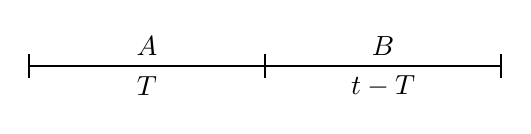
\begin{tikzpicture}

% main line
\draw[thick] (0,0) -- (6,0);

% end ticks
\draw[thick] (0,-0.15) -- (0,0.15);
\draw[thick] (6,-0.15) -- (6,0.15);

% split point
\draw[thick] (3,0.15) -- (3,-0.15);

% labels above (closer)
\node at (1.5,0.25) {$A$};
\node at (4.5,0.25) {$B$};

% labels below (closer)
\node at (1.5,-0.25) {$T$};
\node at (4.5,-0.25) {$t - T$};

\end{tikzpicture}
\end{center}

There are some immediate physical conclusions we can draw. The first is at the end of section \( A \), our final velocity is \( v_{f,A} = AT \), which is also equal to \( v_{0,B} \). Integrate that to get the distance traversed in that first section, which is \( x_{A} = \frac{1}{2}AT^{2} \).

In the second leg, we can immediately deduce that we travel a distance \( x_{B} = 1 - \frac{1}{2}AT^{2} \). To bring the deceleration into the picture, we can also deduce that \( x_{B} \) can be written as 
\[
	x_{B} = AT \!\left( t - T \right) - \frac{1}{2}B \!\left( t - T \right)^{2} 
\]
where \( t - T \) corresponds to the time elapsed during the deceleration phase. This equation stems from the one-dimensional kinematics equations, although you can derive it by integrating the acceleration term twice. Combining our two derivations for \( x_{B} \), we can write
\[
	1 = -\frac{1}{2} \!\left( A + B \right)T^{2} + T \!\left( A + B \right)t - \frac{1}{2}Bt^{2} 
\]
So far, we have one equation and two unknowns. A second equation is needed. We have satisfied the distance constraint, but now we need a \textit{velocity constraint}. Given the initial velocity at the start of section \( B \), the deceleration constant, and knowledge that the final velocity must be zero, then we can build our second equation as such:
\[
	AT - B \!\left( t - T \right) = 0
\]
Isolating \( t \) gives us
\[
	 t = \frac{1}{B}T \!\left( A + B \right)
\]
Finally, we may substitute back into our first equation and solve for the brake time \( T \) to get
\[
	T = \sqrt{\frac{2B}{A \!\left( A + B \right)}} 
\]
In short, the kernel of this problem setup is in understanding that we have two unknowns, \( t \) and \( T \), and thus we will need two constraint equations (distance and velocity) to solve for them.

Note that having the acceleration and deceleration constants given to us as constants simplifies the problem drastically. Otherwise, calculus of variations would have been needed.

\newpage
\subsection{\textsf{8.6 - Convolution (Fourier and Laplace)}}
% QUESTION 1
\qs{8.6.1}{Find the convolution \( \pmb{v * w} \) and also the cyclic convolution \( \pmb{v \circledast w} \):
\begin{enumerate}[label=(\alph*)]
	\item \( \pmb{v} = \!\left( 1,2 \right) \) and \( \pmb{w} = \!\left( 2,1 \right) \)
	\item \( \pmb{v} = \!\left( 1,2,3 \right) \) and \( \pmb{w} = \!\left( 4,5,6 \right) \)
\end{enumerate}}

\begin{enumerate}[label=(\alph*)]
	\item \begin{alignat*}{2}
	      		\pmb{v * w} & = \begin{bmatrix}
	      			1 & \\
	      			2 & 1 \\
	      			 & 2 \\
	      		\end{bmatrix}
			\begin{bmatrix}
				2 \\
				1 \\
			\end{bmatrix} && = 
			\begin{bmatrix}
				2 \\
				5 \\
				2 \\
			\end{bmatrix} \\
			\pmb{v \circledast w} & = \begin{bmatrix}
				1 & 2 \\
				2 & 1 \\
			\end{bmatrix}
			\begin{bmatrix}
				2 \\
				1 \\
			\end{bmatrix} && = 
			\begin{bmatrix}
				4 \\
				5 \\
			\end{bmatrix}
	      \end{alignat*}
	\item \begin{alignat*}{2}
			\pmb{v * w} & = \begin{bmatrix}
				1 &  & \\
				2 & 1 & \\
				3 & 2 & 1 \\
				 & 3 & 2 \\
				 &  & 3 \\
			\end{bmatrix}
			\begin{bmatrix}
				4\\
				5\\
				6\\
			\end{bmatrix} && = 
			\begin{bmatrix}
				4\\
				13\\
				28\\
				27\\
				18\\
			\end{bmatrix} \\
			\pmb{v \circledast w} & = \begin{bmatrix}
				1 & 3 & 2\\
				2 & 1 & 3\\
				3 & 2 & 1\\
			\end{bmatrix}
			\begin{bmatrix}
				4\\
				5\\
				6\\
			\end{bmatrix} && = 
			\begin{bmatrix}
				31\\
				31\\
				28\\
			\end{bmatrix}
	\end{alignat*}
\end{enumerate}
As a rule, the length of the convolution of two vectors of length \( n \) is \( 2n - 1 \). The cyclic convolution of two vectors of length \( n \) is also length \( n \).

\vspace{12pt}

% QUESTION 2
\qs{8.6.2}{Compute the convolution \( \!\left( 1,3,1 \right) * \!\left( 2,2,3 \right) = \!\left( a,b,c,d,e \right) \). To check your answer, add \( a + b + c + d + e \). That total should be 35 since \( 1 + 3 + 1 = 5 \) and \( 2 + 2 + 3 = 7 \) and \( 5 \times 7 = 35 \).}
\[
	\!\left( 1,3,1 \right) * \!\left( 2,2,3 \right) = \begin{bmatrix}
		1 &  & \\
		3 & 1 & \\
		1 & 3 & 1\\
		 & 1 & 3\\
		 &  & 1\\
	\end{bmatrix}
	\begin{bmatrix}
		2\\
		2\\
		3\\
	\end{bmatrix} = 
	\begin{bmatrix}
		2\\
		8\\
		11\\
		11\\
		3\\
	\end{bmatrix}
\]
Confirm that \( 2 + 8 + 11 + 11 + 3 = 35 \).

\vspace{12pt}

% QUESTION 3
\qs{8.6.3}{Multiply \( 1 + 3x + x^{2} \) times \( 2 + 2x + 3x^{2} \) to find \( a + bx + cx^{2} + dx^{3} + ex^{4} \). Your multiplication was the same as the convolution \( \!\left( 1,3,1 \right) * \!\left( 2,2,3 \right) \) in Problem 2. When \( x = 1 \), your multiplication shows why \( 1 + 3 + 1 = 5 \) times \( 2 + 2 + 3 = 7 \) agrees with \( a + b + c + d + e = 35 \).}

\begin{align*}
	\!\left( 1 + 3x + x^{2} \right) \times \!\left( 2 + 2x + 3x^{2} \right) & = \!\left( 2 + 2x + 3x^{2} \right) + \!\left( 6x + 6x^{2} + 9x^{3} \right) + \!\left( 2x^{2} + 2x^{3} + 3x^{4} \right) \\
	 & = 2 + 8x + 11x^{2} + 11x^{3} + 3x^{4}
\end{align*}

% QUESTION 4
\qs{8.6.4}{(Deconvolution) Which vector \( \pmb{v} \) would you convolve with \( \pmb{w} = \!\left( 1,2,3 \right) \) to get \( \pmb{v * w} = \!\left( 0,1,2,3,0 \right) \)? Which \( \pmb{v} \) gives \( \pmb{v \circledast w} = \!\left( 3,1,2 \right) \)?}

The identity vector in this instance is \( \pmb{v} = \!\left( 0,1,0 \right) \). Confirm by calculating
\[
	\pmb{v * w} = \begin{bmatrix}
		 &  & \\
		1 &  & \\
		 & 1 & \\
		 &  & 1\\
		 &  & \\
	\end{bmatrix} 
	\begin{bmatrix}
		1\\
		2\\
		3\\
	\end{bmatrix} = 
	\begin{bmatrix}
		\\
		1\\
		2\\
		3\\
		\\
	\end{bmatrix}
\]
Observing how the elements of \( \pmb{w} \) are permuted, we can conclude
\[
	\pmb{v \circledast w} = \begin{bmatrix}
		 &  & 1\\
		1 &  & \\
		 & 1 & \\
	\end{bmatrix} 
	\begin{bmatrix}
		1\\
		2\\
		3\\
	\end{bmatrix} = 
	\begin{bmatrix}
		3\\
		1\\
		2\\
	\end{bmatrix}
	\quad \implies \quad
	\pmb{v} = 
	\begin{bmatrix}
		\\
		1\\
		\\
	\end{bmatrix}
\]

% QUESTION 5
\qs{8.6.5}{\begin{enumerate}[label=(\alph*)]
	\item For the periodic functions \( f \!\left( x \right) = 4 \) and \( g \!\left( x \right) = 2 \cos\!\left(x\right) \), show that \( f * g \) is \textbf{zero} (the zero function)! 
	\item In frequency space (\( k \)-space) you are multiplying the Fourier coefficients of \( 4 \) and \( 2 \cos\!\left(x\right) \). Those coefficients are \( c_{0} = 4 \) and \( d_{1} = d_{-1} = 1 \). Therefore every product \( c_{k}d_{k} \) is \underline{\qquad}.
\end{enumerate}}

\begin{enumerate}[label=(\alph*)]
	\item Calculate
	\[
		\!\left( f * g \right)\!\left( x \right) = \int^{2 \pi}_{0} g \!\left( y \right)f \!\left( x - y \right) \, dy = \int^{2 \pi}_{0} 8 \cos\!\left(y\right) \, dy = 8 \sin\!\left(y\right) \Big|^{2 \pi}_{0} = 0 
	\]
	\item Every product \( c_{k}d_{k} = 0 \).
\end{enumerate}

% QUESTION 6
\qs{8.6.6}{For periodic functions \( f = \sum c_{k}e^{ikx} \) and \( g = \sum d_{k}e^{ikx} \), the Fourier coefficients of \( f * g \) are \( \pmb{2 \pi c_{k}d_{k}} \). Test this factor \( 2 \pi \) when \( f \!\left( x \right) = 1 \) and \( g \!\left( x \right) = 1 \) by computing \( f * g \) from its definition (4).}

\[
	\!\left( f * g \right)\!\left( x \right) = \int^{2 \pi}_{0} dy = 2 \pi  
\]

% QUESTION 7
\qs{8.6.7}{Show by integration that the periodic convolution 
\[ 
	\int^{2 \pi}_{0} \cos\!\left(x\right) \cos\!\left(t - x\right) \, dx
\]
is \( \pi \cos\!\left(t\right) \).

In \( k \)-space you are squaring Fourier coefficients \( c_{1} = c_{-1} = \frac{1}{2} \) to get \( \frac{1}{4} \) and \( \frac{1}{4} \); these are the coefficients of \( \frac{1}{2}\cos\!\left(t\right) \). The \( 2 \pi \) in Problem 6 makes \( \pi \cos\!\left(t\right) \) correct.}

Calculate
\begin{align*}
	\int^{2 \pi}_{0} \cos\!\left(x\right) \cos\!\left(t - x\right) \, dx & = \frac{1}{2}\int^{2 \pi}_{0} \!\left[ \cos\!\left(2x - t\right) + \cos\!\left(t\right) \right] \, dx \\
									     & = \frac{1}{4}\sin\!\left(2x - t\right) + \frac{1}{2}x \cos\!\left(t\right) \Big|^{2 \pi}_{0} \\
									     & = \pi \cos\!\left(t\right) 
\end{align*}

% QUESTION 8
\qs{8.6.8}{Explain why \( f * g \) is the same as \( g * f \) (periodic or infinite convolution).}

One intuitive explanation is to consider two sheets of paper, and overlapping one with the other. It does not matter which sheet is moved to overlap with the other; the overlapped area will be the same irrespective of that choice.

Mathematically, a simple variable substitution \( \tau = x - y \) allows one to switch between \( f * g \) or \( g * f \). Additionally, convolution in function space corresponds to multiplication in frequency space, and since the product of coefficients commutes, it follows that convolution also commutes.

\newpage

% QUESTION 9
\qs{8.6.9}{What 3 by 3 circulant matrix \( C \) produces cyclic convolution with the vector \( \pmb{c} = \!\left( 1,2,3 \right) \)? Then \( C \pmb{d} \) equals \( \pmb{c \circledast d} \) for every vector \( \pmb{d} \). Compute \( \pmb{c \circledast d} \) for \( \pmb{d} = \!\left( 0,1,0 \right) \).}

\[
	C = \begin{bmatrix}
		1 & 3 & 2\\
		2 & 1 & 3\\
		3 & 2 & 1\\
	\end{bmatrix} \quad \implies \quad
	C \pmb{d} = \begin{bmatrix}
		1 & 3 & 2\\
		2 & 1 & 3\\
		3 & 2 & 1\\
	\end{bmatrix} 
	\begin{bmatrix}
		\\
		1\\
		\\
	\end{bmatrix} = 
	\begin{bmatrix}
		3\\
		1\\
		2\\
	\end{bmatrix} = 
	\pmb{c \circledast d}
\]

% QUESTION 10
\qs{8.6.10}{What 2 by 2 circulant matrix \( C \) produces cyclic convolution with \( \pmb{c} = \!\left( 1,1 \right) \)? Show in four ways that this \( C \) is not invertible. Deconvolution is impossible.
\begin{enumerate}[label=(\arabic*)]
	\item Find the determinant of \( C \).
	\item Find the eigenvalues of \( C \).
	\item Find \( \pmb{d} \) so that \( C \pmb{d} = \pmb{c \circledast d} \) is zero.
	\item \( F \pmb{c} \) has a zero component.
\end{enumerate}}

The circulant matrix is
\[
	C = \begin{bmatrix}
		1 & 1\\
		1 & 1\\
	\end{bmatrix} 
\]
\begin{enumerate}[label=(\arabic*)]
	\item \( \det C = 1 - 1 = 0 \), zero determinant implies non-invertibility.
	\item \[
		\det \begin{bmatrix}
			1 - \lambda & 1\\
			1 & 1 - \lambda\\
		\end{bmatrix} = \!\left( 1 - \lambda \right)^{2} - 1 = 0 \quad \implies \quad \lambda_{1,2} = 2, 0
	\]
	A zero eigenvalue implies non-invertibility.
	\item Observe that
	\[
		\pmb{d} = \begin{bmatrix}
			1\\
			-1\\
		\end{bmatrix} \quad \implies \quad C \pmb{d} =
		\begin{bmatrix}
			1 & 1\\
			1 & 1\\
		\end{bmatrix}
		\begin{bmatrix}
			1\\
			-1\\
		\end{bmatrix} = 
		\begin{bmatrix}
			0\\
			0\\
		\end{bmatrix} = 
		\pmb{c \circledast d}
	\]
	which implies linear dependence in the rows and thus non-invertibility.
	\item \[
		F \pmb{c} = \begin{bmatrix}
			1 & 1\\
			1 & w\\
		\end{bmatrix} 
		\begin{bmatrix}
			1\\
			1\\
		\end{bmatrix}
		= 
		\begin{bmatrix}
			2\\
			1 + w\\
		\end{bmatrix}
		= 
		\begin{bmatrix}
			2\\
			0\\
		\end{bmatrix}
	\]
	where \( w = e^{-\pi i} \). Observe that \( \pmb{c} \) is one of the eigenvectors (corresponding to eigenvalue \( \lambda = 2 \)), and the Fourier matrix times that eigenvector restores the eigenvalues.
\end{enumerate}

% QUESTION 11
\qs{8.6.11}{\begin{enumerate}[label=(\alph*)]
	\item Change \( b \!\left( x \right) * \delta \!\left( x - 1 \right) \) to a multiplication \( \hat{b}\hat{d} \). Transform the box function
	\[
		b \!\left( x \right) = \!\left\{ 1 \text{ for } 0 \le x \le 1 \right\} \text{ to } \hat{b}\!\left( k \right) = \int^{1}_{0} e^{-ikx} \, dx  
	\]
	The shifted delta transforms to 
	\[
		\hat{d}\!\left( k \right) = \int \delta \!\left( x - 1 \right)e^{-ikx} \, dx 
	\]
	\item Show that your result \( \hat{b}\hat{d} \) is the transform of a shifted box function. Then convolution with \( \delta \!\left( x - 1 \right) \) shifts the box.
\end{enumerate}}

\begin{enumerate}[label=(\alph*)]
	\item Convolving without working in frequency space gives us
	\[
		 b \!\left( x \right) * \delta \!\left( x - 1 \right) = \int^{\infty}_{-\infty} b \!\left( y \right) \delta \!\left( x - 1 - y \right) \, dy = b \!\left( x - 1 \right) = \begin{cases}
		 	1, & 1 \le x \le 2 \\
		 	0, & \text{else} \\
		 \end{cases}
	\]
	which corresponds to a one-step shift in \( b \!\left( x \right) \). Meanwhile, multiplication in frequency space gives
	\[
		\hat{b}\hat{d} = \int^{1}_{0} e^{-ikx} \, dx \int^{\infty}_{-\infty} \delta \!\left( x - 1 \right)e^{-ikx} \, dx = \!\left[ -\frac{e^{-ikx}}{ik} \Big|^{1}_{0} \right]e^{-ik} = \!\left[ \frac{1 - e^{-ik}}{ik} \right]e^{-ik}
	\]
	\item The transform of the one-step shifted \( b \!\left( x \right) \) is
	\[
		\hat{b}\!\left( k \right) = \int^{2}_{1} e^{-ikx} \, dx = \!\left[ \frac{1 - e^{-ik}}{ik} \right]e^{-ik} 
	\]
\end{enumerate}

% QUESTION 12
\qs{8.6.12}{Take the Laplace transform of these equations to find the transfer function \( G \!\left( s \right) \):
\begin{enumerate}[label=(\alph*)]
	\item \( Ay'' + By' + Cy = \delta \!\left( t \right) \)
	\item \( y' - 5y = \delta \!\left( t \right) \)
	\item \( 2y \!\left( t \right) - y \!\left( t - 1 \right) = \delta \!\left( t \right) \)
\end{enumerate}}
Assume zero for all initial conditions.
\begin{enumerate}[label=(\alph*)]
	\item \( As^{2}Y + BsY + CY = 1 \quad \implies \quad Y \!\left( s \right) = \displaystyle{\frac{1}{As^{2} + Bs + C}} \)
	\item \( sY - 5Y = 1 \quad \implies \quad Y \!\left( s \right) = \displaystyle{\frac{1}{s - 5}} \)
	\item \( 2Y - Ye^{-s} = 1 \quad \implies \quad Y \!\left( s \right) = \displaystyle{\frac{1}{2 - e^{-s}}} \)
\end{enumerate}

% QUESTION 13
\qs{8.6.13}{Take the Laplace transform of \( y'''' = \delta \!\left( t \right) \) to find \( Y \!\left( s \right) \). From the Transform Table in Section 8.5 find \( y \!\left( t \right) \). You will see \( y''' = 1 \) and \( y'''' = 0 \). But \( y \!\left( t \right) = 0 \) for negative \( t \), so your \( y''' \) is actually a unit step function and your \( y'''' \) is actually \( \delta \!\left( t \right) \).}

We have \( s^{4}Y = 1 \) which gives us
\[
	Y \!\left( s \right) = \frac{1}{s^{4}} 
\]
This corresponds to \( y \!\left( t \right) = t^{3} / 6 \). By the discontinuity at \( t = 0 \) since \( y \!\left( t \right) = 0 \) for negative \( t \), we must have \( y'''' = \delta \!\left( t \right) \) and not \( y'''' = 0 \).

\vspace{12pt}

% QUESTION 14
\qs{8.6.14}{Solve these equations by Laplace transform to find \( Y \!\left( s \right) \). Invert that transform with the Table in Section 8.5 to recognize \( y \!\left( t \right) \).
\begin{enumerate}[label=(\alph*)]
	\item \( y' - 6y = e^{-t}, y \!\left( 0 \right) = 2 \)
	\item \( y'' + 9y = 1, y \!\left( 0 \right) = y'\!\left( 0 \right) = 0 \)
\end{enumerate}}

\begin{enumerate}[label=(\alph*)]
	\item \( sY - 2 - 6Y = \displaystyle{\frac{1}{s + 1}} \quad \implies \quad Y \!\left( s \right) = \displaystyle{\frac{1}{\!\left( s + 1 \right)\!\left( s - 6 \right)} + \frac{2}{s - 6}} \)

	By partial fractions,
	\[
		Y \!\left( s \right) = -\frac{1}{7 \!\left( s + 1 \right)} + \frac{15}{7 \!\left( s - 6 \right)}
	\]
	which corresponds to time domain solution
	\[
		y \!\left( t \right) = \frac{15}{7}e^{6t} - \frac{1}{5}e^{-t}
	\]
	\item \( s^{2}Y + 9Y = \displaystyle{\frac{1}{s}} \quad \implies \quad Y \!\left( s \right) = \frac{1}{s \!\left( s^{2} + 9 \right)} \)

	By partial fractions,
	\[
		Y \!\left( s \right) = \frac{1}{3s} - \frac{s}{3 \!\left( s^{2} + 3 \right)} 
	\]
	which corresponds to time domain solution
	\[
		y \!\left( t \right) = \frac{1}{9} - \frac{1}{9}\cos\!\left(3t\right)  
	\]
\end{enumerate}

\newpage

% QUESTION 15
\qs{8.6.15}{Find the Laplace transform of the shifted step \( H \!\left( t - 3 \right) \) that jumps from 0 to 1 at \( t = 3 \). Solve \( y' - ay = H \!\left( t - 3 \right) \) with \( y \!\left( 0 \right) = 0 \) by finding the Laplace transform \( Y \!\left( s \right) \) and then its inverse transform \( y \!\left( t \right) \): one part for \( t < 3 \), second part for \( t \ge 3 \).}
\[
	sY - aY = \frac{e^{-3s}}{s} \quad \implies \quad Y \!\left( s \right) = \frac{e^{-3s}}{s \!\left( s - a \right)} = e^{-3s}\!\left[ -\frac{1}{as} + \frac{1}{a \!\left( s - a \right)} \right]
\]
which corresponds to time domain solution
\[
	y \!\left( t \right) = \frac{1}{a} \!\left[ e^{a \!\left( t - 3 \right)} - 1 \right] H \!\left( t - 3 \right)
\]

% QUESTION 16
\qs{8.6.16}{Solve \( y' = 1 \) with \( y \!\left( 0 \right) = 4 \)-- a trivial question. Then solve this problem the slow way by finding \( Y \!\left( s \right) \) and inverting that transform.}

The solution can be derived on inspection: \( y \!\left( t \right) = t + 4 \). By transforms, we have
\[
	sY - 4 = \frac{1}{s} \quad \implies \quad Y \!\left( s \right) = \frac{1}{s^{2}} + \frac{4}{s} 
\]
which has time domain solution (as expected)
\[
	y \!\left( t \right) = t + 4 
\]

% QUESTION 17
\qs{8.6.17}{The solution \( y \!\left( t \right) \) is the convolution of the input \( f \!\left( t \right) \) with what function \( g \!\left( t \right) \)?
\begin{enumerate}[label=(\alph*)]
	\item \( y' - ay = f \!\left( t \right) \) with \( y \!\left( 0 \right) = 3 \)
	\item \( y' - \!\left( \text{integral of } y \right) = f \!\left( t \right) \)
\end{enumerate}}

The task is to identify the transfer function \( G \!\left( s \right) \) and its corresponding Green's function \( g \!\left( t \right) \).

\begin{enumerate}[label=(\alph*)]
	\item \( sY - 3 - aY = F \!\left( s \right) \quad \implies \quad Y \!\left( s \right) = \displaystyle{\frac{F \!\left( s \right) + 3}{s - a}} \) which has time domain solution
	\[
		y \!\left( t \right) = f \!\left( t \right) * e^{at} + 3e^{at} 
	\]
	Appreciate the elegance of this operation: even in ignorance of \( f \!\left( t \right) \), we may still write a solution \( y \!\left( t \right) \) thanks to the switch between the \( s \)- and \( t \)-domains corresponding to a switch between multiplication and convolution.
	\item Two ways to solve: first, attempt to derive the Laplace transform of \( \int y \, dt \):
	\[
		\mathcal{L}\!\left[ \int y \!\left( T \right) \, dT \right] = \int^{\infty}_{0} \!\left[ \int^{t}_{0} y \!\left( T \right) \, dT \right]e^{-st} \, dt 
	\]
	Solve by integration by parts. Let \( u = \displaystyle{\int^{t}_{0} y \!\left( T \right) \, dT } \) and \( dv = e^{-st} \, dt \). Then \( du = y \!\left( t \right) \) and \( v = -e^{-st} / s \). We have
	\begin{align*}
		\mathcal{L}\!\left[ \int y \!\left( T \right) \, dT \right] & = -\frac{e^{-st}}{s} \int^{t}_{0} y \!\left( T \right) \, dT \Big|^{\infty}_{0} + \int^{\infty}_{0} y \!\left( t \right) \frac{e^{-st}}{s} \, dt \\
		 & = \frac{Y \!\left( s \right)}{s}
	\end{align*}
	A convenient result: differentiation produces \( s \), and integration gives us \( 1 / s \). The rest is straightforward.
	\[
		sY - \frac{Y}{s} = F \!\left( s \right) \quad \implies \quad Y \!\left( s \right) = \frac{F \!\left( s \right)}{s - \frac{1}{s}}, \quad G \!\left( s \right) = \frac{1}{s - \frac{1}{s}}
	\]
	It is clearer if we rewrite \( G \!\left( s \right) \) as 
	\[
		G \!\left( s \right) = \frac{s}{s^{2} - 1} 
	\]
	which is the transform of \( g \!\left( t \right) = \cos\!\left(it\right) \).
	Alternatively, we can differentiate through to annihlate the integral. Equivalently, we solve
	\[
		y'' - y = f'\!\left( t \right) 
	\]
	Applying the transform gets us
	\[
		s^{2}Y - Y = s F \!\left( s \right) \quad \implies \quad Y \!\left( s \right) = \frac{s F \!\left( s \right)}{s^{2} - 1}
	\]
	Either way, we derive \( y \!\left( t \right) = f \!\left( t \right) * \cos\!\left(it\right) \).
\end{enumerate}

% QUESTION 18
\qs{8.6.18}{For \( y' - ay = f \!\left( t \right) \) with \( y \!\left( 0 \right) = 3 \), we could replace that initial value by adding \( 3 \delta \!\left( t \right) \) to the forcing function \( f \!\left( t \right) \). Explain that sentence.}

In the \( s \)-domain, the transform of \( y' \) gets us \( sY - y \!\left( 0 \right) \). This produces \( 3 \) on the right-hand side. Equivalently, the transform of \( 3 \delta \!\left( t \right) \) is \( 3 \), landing us in the same place.

\newpage

% QUESTION 19
\qs{8.6.19}{What is \( \delta \!\left( t \right) * \delta \!\left( t \right) \)? What is \( \delta \!\left( t - 1 \right) * \delta \!\left( t - 2 \right) \)? What is \( \delta \!\left( t - 1 \right) \) \textit{times} \( \delta \!\left( t - 2 \right) \)?}

Equivalently, in \( s \)-space we have \( 1 \cdot 1 = 1 \), which maps back to \( \delta \!\left( t \right) \) in \( t \)-space. In the second equation, we have \( e^{-s} \cdot e^{-2s} = e^{-3s} \) in \( s \)-space, or \( \delta \!\left( t - 3 \right) \) in \( t \)-space. Lastly, \( \delta \!\left( t - 1 \right) \delta \!\left( t - 2 \right) = 0 \), as there is no \( t \) that satisfies a non-zero product of these delta functions.

\vspace{12pt}

% QUESTION 20
\qs{8.6.20}{By Laplace transform, solve \( y' = y \) with \( y \!\left( 0 \right) = 1 \) to find a very familiar \( y \!\left( t \right) \).}

\[
	sY - 1 = Y \quad \implies \quad Y \!\left( s \right) = \frac{1}{s - 1} \quad \implies \quad y \!\left( t \right) = e^{t} 
\]

% QUESTION 21
\qs{8.6.21}{By Fourier transform as in (9), solve \( -y'' + y = \) box function \( b \!\left( x \right) \) on \( 0 \le x \le 1 \).}

Derive
\[
	-\!\left( ik \right)^{2}\hat{y} + \hat{y} = \int^{1}_{0} e^{-ikx} \, dx = \frac{1 - e^{-ik}}{ik} \quad \implies \quad \hat{y} = \frac{1 - e^{-ik}}{ik \!\left( k^{2} + 1 \right)}
\]
Decomposing \( \hat{y} \) into \( F \!\left( s \right)G \!\left( s \right) \), we have

\begin{align*}
	\hat{y} = \left( \frac{1 - e^{-ik}}{ik} \right)\left( \frac{1}{k^{2} + 1} \right) \quad \implies \quad y(x) & = \left[ H(x) - H(x - 1) \right] * \frac{1}{2}e^{-|x|} \\
		      & = \frac{1}{2} \int_{0}^{1} e^{-|x - y|} \, dy
\end{align*}
This is the transform method for solving this equation. The alternative is to solve the equation piecewise, and deriving the coefficients from the junctions at \( x = 0 \) and \( x = 1 \). For students of quantum mechanics, you may find this reminiscent of solving the wave equation in ``particle-in-a-box'' scenarios.

\vspace{12pt}

% QUESTION 22
\qs{8.6.22}{There is a big difference in the solutions to \( y'' + By' + Cy = f \!\left( x \right) \), between the cases \( B^{2} < 4C \) and \( B^{2} > 4C \). Solve \( y'' + y = \delta \) and \( y'' - y = \delta \) with \( y \!\left( \pm \infty \right) = 0 \).}

Since we look at the full real line, we apply the Fourier transform to derive
\[
	\!\left( ik \right)^{2}\hat{y} + \hat{y} = 1 \quad \implies \quad \hat{y} = \frac{1}{1 - k^{2}}
\]
Taking the inverse Fourier transform gives
\[
	y \!\left( x \right) = \frac{1}{2}\sin\!\left(\abs{x}\right)  
\]
For this periodic function, we do not impose \( y \!\left( \pm \infty \right) = 0 \) at the extremes.

In the second question, derive
\[
	\!\left( ik \right)^{2}\hat{y} - \hat{y} = 1 \quad \implies \quad \hat{y} = -\frac{1}{k^{2} + 1} 
\]
which corresponds to \( x \)-domain function
\[
	y \!\left( x \right) = -\frac{1}{2}e^{-\abs{x}} 
\]
and in this case, we see that the boundary conditions \( y \!\left( \pm \infty \right) = 0 \) hold.

\vspace{12pt}

% QUESTION 23
\qs{8.6.23}{(\textit{Review}) Why do the constant \( f \!\left( t \right) = 1 \) and the unit step \( H \!\left( t \right) \) have the same Laplace transform \( 1 / s \)? Answer: Because the transform does not notice \underline{\qquad}.}

The Laplace transform does not notice \( f \!\left( t \right) \) for \( t < 0 \), i.e. \( f \!\left( t \right) = 0 \) on that domain.

\end{document}
